\documentclass[12pt,a4paper]{article}
\usepackage[pdftex]{graphicx} %for embedding images
\usepackage{url} %for proper url entries
\usepackage[bookmarks, colorlinks=false, pdfborder={0 0 0}, pdftitle={<pdf title here>}, pdfauthor={<author's name here>}, pdfsubject={<subject here>}, pdfkeywords={<keywords here>}]{hyperref} 
\usepackage{amsmath,amsthm,amssymb,amsfonts}
\usepackage{lipsum}
\usepackage[margin=1in,includefoot]{geometry}
\usepackage{multirow}%test cases
\usepackage{float}
\usepackage{amssymb}
\newcommand{\checkbox}{$\square$}
\newcommand\fillin[1][3cm]{\makebox[#1]{\dotfill}}
%for refferennce numbering
\usepackage[nottoc,notlot,notlof]{tocbibind}
%for cant show section number
\usepackage{caption}%for caption number delete
\usepackage{CJKutf8}
\newcommand{\zh}[1]{\begin{CJK}{UTF8}{gbsn}#1\end{CJK}}

%left allignment
\usepackage{ragged2e}

%font size
\usepackage[T1]{fontenc}
\usepackage[utf8]{inputenc}
\pdfmapline{= rjvnr8t Verdana " winfontsT1Encoding ReEncodeFont " <[winfonts256.enc <verdana.ttf}
\usepackage{newtxtext,newtxmath}

\usepackage{verbatim}

%tab
\newcommand\tab[1][1cm]{\hspace*{#1}}
% Code segment
\usepackage{listings}
\usepackage{color}

%Header footer
\usepackage{geometry,fancyhdr}
\pagestyle{fancy}
\fancyhf{}% Clear header/footer
\chead{%
  Shenyang Aerospace University Graduation Design(Thesis)
}
\cfoot{\thepage}
\setlength{\headheight}{24pt}

\definecolor{dkgreen}{rgb}{0,0.6,0}
\definecolor{gray}{rgb}{0.5,0.5,0.5}
\definecolor{mauve}{rgb}{0.58,0,0.82}

\usepackage{array}

\newcolumntype{M}[1]{>{\centering\arraybackslash}m{#1}}
\newcolumntype{N}{@{}m{0pt}@{}}

%Title Chapter
\usepackage{blindtext}
\usepackage{sectsty}
\sectionfont{\centering}



\lstset{frame=tb,
  language=Java,
  aboveskip=3mm,
  belowskip=3mm,
  showstringspaces=false,
  columns=flexible,
  basicstyle={\small\ttfamily},
  numbers=none,
  numberstyle=\tiny\color{gray},
  keywordstyle=\color{blue},
  commentstyle=\color{dkgreen},
  stringstyle=\color{mauve},
  breaklines=true,
  breakatwhitespace=true,
  tabsize=3
}

\begin{document}
	%\renewcommand\bibname{References} 		%Renames "Bibliography" to 				"References"
	%\begin{titlepage}
\begin{center}
	\centering
	
\includegraphics[width=0.15\textwidth]{/home/basedul/Documents/Report-writing-using-latex/ResturentManagementSystemReport/BasedulAppIcon.png}\par\vspace{1cm}
	{\scshape\LARGE Columbidae University \par}
	\vspace{1cm}
	{\scshape\Large Final year project\par}
	\vspace{1.5cm}
	{\huge\bfseries Pigeons love doves\par}
	\vspace{2cm}
	{\Large\itshape John Birdwatch\par}
	\vfill
	supervised by\par
	Dr.~Mark \textsc{Brown}

	\vfill

% Bottom of the page
	{\large \today\par}
\end{center}
\end{titlepage}
	%height=4in
	\begin{titlepage}
	\begin{center}
	\centering
	\noindent\begin{minipage}{0.3\textwidth}% adapt widths of minipages to your needs

\includegraphics[width=\linewidth]{/home/basedul/Documents/Report-writing-using-latex/ResturentManagementSystemReport/titlepic.png}
\end{minipage}
\hfill
\begin{minipage}{0.6\textwidth}
%\raggedleft
{\fontsize{24}{10}\fontfamily{ptm}\selectfont \textbf{Graduation Thesis}
}

\end{minipage}

\par\vspace{0cm}
	{\fontsize{22}{10}\fontfamily{ptm}\selectfont \begin{center}
	\textbf{Asian Restaurant Management Application}
	\end{center}}
	{\fontsize{20}{10}\fontfamily{ptm}\selectfont \begin{center}
	\zh{亚洲餐厅管理应用}
	\end{center}}
	\vspace{1cm}
	
	\begin{table}[ht]
	\center
	\begin{tabular}{M{4cm}M{8cm}N}
	
	{\fontsize{16}{10}\fontfamily{ptm}\selectfont \begin{flushleft}
	Major
	\end{flushleft}} & {\fontsize{16}{10}\fontfamily{ptm}\selectfont \begin{flushleft}
	Computer Science and Technology
	\end{flushleft}}&\\[0.1pt]
	
	{\fontsize{16}{10}\fontfamily{ptm}\selectfont \begin{flushleft}
	Class
	\end{flushleft}} & {\fontsize{16}{10}\fontfamily{ptm}\selectfont \begin{flushleft}
	140104
	\end{flushleft}}&\\[0.1pt]
	
	{\fontsize{16}{10}\fontfamily{ptm}\selectfont \begin{flushleft}
	Stuent No.
	\end{flushleft}} & {\fontsize{16}{10}\fontfamily{ptm}\selectfont \begin{flushleft}
	14031274
	\end{flushleft}}&\\[0.1pt]
	
	\fontsize{16}{10}\fontfamily{ptm}\selectfont{\begin{flushleft}
	Name
	\end{flushleft}} & \fontsize{16}{10}\fontfamily{ptm}\selectfont{\begin{flushleft}
	Hossain Syed Abir(\zh{阿贝尔})
	\end{flushleft}}&\\[0.1pt]
	
	\fontsize{16}{10}\fontfamily{ptm}\selectfont{\begin{flushleft}
	Supervisor
	\end{flushleft}} & \fontsize{16}{10}\fontfamily{ptm}\selectfont{\begin{flushleft}
	Liang Zhao
	\end{flushleft}}&\\[0.1pt]
	
	\end{tabular}
	\end{table}	
	
	
	\vspace{1cm}
	{\fontsize{18}{10}\fontfamily{ptm}\selectfont \MakeUppercase{Shenyang Aerospace University} \par}
	\vspace{0.5cm}
	\begin{comment}\vspace{1cm}
	{\scshape\Large Final year project\par}
	\vspace{1.5cm}\end{comment}
	
	%{\Large\itshape Hossain Syed Abir\par}
	\begin{comment}\vfill
	Supervised by\par
	\textsc{Liang Zhao}

	\vfill
	\end{comment}

% Bottom of the page
	{\fontsize{16}{1}\fontfamily{ptm}\selectfont \today\par}
\end{center}
\end{titlepage}

\begin{titlepage}
	{\fontsize{22}{10}\fontfamily{ptm}\selectfont \begin{center}
	\textbf{Asian Restaurant Management Application}
	\end{center}}
	{\fontsize{20}{10}\fontfamily{ptm}\selectfont \begin{center}
	\zh{亚洲餐厅管理应用}
	\end{center}}
	\vspace{6cm}
	
	\begin{table}[ht]
	\center
	\begin{tabular}{M{4cm}M{8cm}N}
	
	{\fontsize{16}{10}\fontfamily{ptm}\selectfont \begin{flushleft}
	Major
	\end{flushleft}} & {\fontsize{16}{10}\fontfamily{ptm}\selectfont \begin{flushleft}
	Computer Science and Technology
	\end{flushleft}}&\\[0.1pt]
	
	{\fontsize{16}{10}\fontfamily{ptm}\selectfont \begin{flushleft}
	Class
	\end{flushleft}} & {\fontsize{16}{10}\fontfamily{ptm}\selectfont \begin{flushleft}
	140104
	\end{flushleft}}&\\[0.1pt]
	
	{\fontsize{16}{10}\fontfamily{ptm}\selectfont \begin{flushleft}
	Stuent No.
	\end{flushleft}} & {\fontsize{16}{10}\fontfamily{ptm}\selectfont \begin{flushleft}
	14031274
	\end{flushleft}}&\\[0.1pt]
	
	\fontsize{16}{10}\fontfamily{ptm}\selectfont{\begin{flushleft}
	Name
	\end{flushleft}} & \fontsize{16}{10}\fontfamily{ptm}\selectfont{\begin{flushleft}
	Hossain Syed Abir(\zh{阿贝尔})
	\end{flushleft}}&\\[0.1pt]
	
	\fontsize{16}{10}\fontfamily{ptm}\selectfont{\begin{flushleft}
	Supervisor
	\end{flushleft}} & \fontsize{16}{10}\fontfamily{ptm}\selectfont{\begin{flushleft}
	Liang Zhao
	\end{flushleft}}&\\[0.1pt]
	
	\end{tabular}
	\end{table}	
	
	\newpage
	{\fontsize{18}{5}\fontfamily{ptm}\selectfont \begin{center}
	\MakeUppercase{Shenyang Aerospace University}
	\end{center} \par}
	\vspace{0.15cm}

% Bottom of the page
	{\fontsize{16}{5}\fontfamily{ptm}\selectfont \begin{center}
	\today
	\end{center}\par}
	\vspace{0.15cm}
	{\fontsize{16}{5}\fontfamily{ptm}\selectfont \begin{center}
	\textbf{Declaration}
	\end{center}\par}
	\vspace{1cm} 

\RaggedRight \fontsize{14}{10}\fontfamily{ptm}\selectfont To the best of my knowledge and belief, I certify that this thesis does not:\\
\begin{itemize}
	\item[I.] Incorporate any material previously submitted for a degree or diploma in any institution of higher education without acknowledgement.
	\item[II.] Contain any material previously published or written by other person except where due reference is made in the text.
	\item[III.] Contain any defamatory material.
\end{itemize}
I also grant permission to Shenyang Aerospace University to make duplicate copies of my thesis as required.	\\
\vspace{1cm}


\begin{flushleft}
Signature\fillin[4cm]
\end{flushleft}
Date\fillin[5cm] 
	
\end{titlepage}	

	
	\begin{titlepage}
		%\cfoot{\thepage}
		\centering 
		{ \bfseries Abstract}\\
		\vspace{0.6cm}
		\RaggedRight \tab The project {\bfseries Asian Restaurant Management Application is implemented} to reduce the
manual work and enhances the accuracy of work in a restaurant. This software has been made
in a user friendly interface. This project is also designed with full consideration to help the
users in an easy manner without any unnecessary wastage of time. This application can be
implemented in big restaurant where customers can order their food from their table using
application. The application consists of various food varieties available in the restaurant.
Through the ordering form, the customer can simply click and order the food even from
home. This application entirely reduces the unnecessary time waste inside the hotel as well as
it reduces unnecessary noise. This report documents the process of designing, developing and
testing a software application to be used in a restaurant; usually given the name restaurant
management application. The restaurant management application is there to help
communication between all teams within a restaurant by minimizing the probability of human
errors. This project serves the best way of maintaining customer’s information and caters
their needs. The application is designed and implemented with client and server mode. This is
an integrated application which contains both the user component (used by client to sign up,
sign in, sign out the application, modifying personal information, browse the detail
information of a food, query a specified cuisine according to the name or type, write user
experience or comment on the dish and submit satisfaction score, user get reward points after
sharing their experiences) and the admin component (used by the administrators for
performing admin level functions such as sign up, sign in, sign out the application, modifying
personal information, managing the order list, adding new cuisine items). This application is
successfully running for the restaurant management. Asian Restaurant Management
Application is a java application designed with Java technique and MySQL server as the
database of the application.\\
\vspace{0.8cm}
{\bfseries Key Words: } Java technique, Wamp server, MySQL Database.
	\newpage
	\thispagestyle{empty}
	\centering\zh{摘 要}\\
	\vspace{0.5cm}
	
	\zh{“亚洲餐厅管理应用”项目旨在减少人工劳动,提高餐厅工作的准确性。这个软件是用户友好的界面制作
的。这个系统由餐馆里各种各样的食物组成。通过订购表单,客户可以简单地点击和订购食品,甚至在
家里。这份报告记录了设计、开发和测试一个在餐馆使用的软件系统的过程;通常给出餐馆管理系统的
名称。餐厅管理系统通过最小化人为错误的概率来帮助餐厅内所有团队之间的沟通。这个项目是维护客
户信息和满足客户需求的最佳方式。系统采用客户机和服务器模式设计和实现。这是一个集成的系统应
用程序,它包含两个用户组件(由客户端用于注册、登录、签出应用程序、修改个人信息、浏览食物的
细节信息、根据名称或类型查询指定菜肴、在菜肴上写用户体验或评论以及提交满意度评分),用户在
分享他们的经验之后获得奖励积分)和管理组件(管理员用于执行管理级功能,例如注册、登录、签出
应用程序、修改个人信息、管理订单列表、添加新的菜肴项目)。此应用程序已成功用于餐厅管理。亚
洲餐厅管理应用程序是以Java技术和MySQL Server为系统的数据库设计的Java应用程序。\linebreak}\\

\RaggedRight\zh{\bfseries{关键词:}}\zh{亚洲餐厅管理应用,Java技术,MySQL服务器,数据库}
	\end{titlepage}
	
	\pagenumbering{roman} %numbering before main content starts
	\newpage
	\tableofcontents
	\newpage
	\listoffigures
	\newpage
	\listoftables
	
	\newpage
	\pagenumbering{arabic} %reset numbering to normal for the main content
	
	\section{Introduction}
	%{\bfseries \Large INTODUCTION}\\
	\tab The concept of restaurant table order management system, since it is java application, I will keep everything as simple as possible. The project consists in an java application that can be used by employees in a restaurant to handle the clients, their orders and can help them easily find free tables or place orders. This application, created mainly for proof of proper user-java interaction. The restaurant menu is organized by categories (appetizers, soups,fig salads, entrees etc.) of menu items. Each menu item has a chef, preparation instructions and associated ingredients. The ingredients are identified by their ingredient id and the quality of the ingredient needed to prepare a particular recipe, the unit of measure and a name.
\\
\tab "Restaurant Management System(RMS)" is java application to restaurant management. This system wake to provide service facility to rastaurant and also to the customer. The services that are provided is food ordering and home delivery by the customer through the system, customer information management and waiter information management, menu information management and report. Main objective build the system, ordering, and home delivery management will become easier and systematic to replace traditional system.

	
	\subsection{Project Objectves}
	\tab We are stuck with technology when what we really want is just stuff that works. With
the current paradigm shift in technological field, there is an urgent need to embrace and
appreciate the power of technology.Restaurant sector remains vigilant to face the challenges
of change by employing a new strategy that facilities easy management system that can
simplify work for the restaurant managers so that all their work can be efficient and effective.
The general objectives of the study is to develop a reliable, convenient and accurate Ordering System.\\
The study has the following specific objectives:
		\begin{itemize}
			\item To develop a system that will surely satisfied the customer service.
			\item To design a system able to accommodate huge amount of orders at a time.
			\item  To evaluate its performance and acceptability in terms of security, user-friendliness, accuracy and reliability.
			\item  To improve the communication between the client and the server and minimize the time of ordering.
		\end{itemize}
		
\RaggedRight One of the main objectives of a restaurant to ensure customer satisfaction. Manual listing of orders by the waiters/waitresses may result to slow response in customer service. Hence, if the restaurant uses the proposed system, manipulation of orders to the customers be so easy and choosing the desired menu.

	\subsection{Project Requirements Analysis}
	\tab Project requirements analysis are important stage in the system development. It
determines the functions of the whole system integrity and stability. Software requirements
analysis is an ongoing process of understanding and progressive refinement. Through
requirements analysis, design functions of the management system as below.
			\begin{itemize}
				\item[a.]User management. User can register (Manager or customer), login and logout the website;
				\item[b.]Adding a food. Manager can add new food information for showing to customer.
				\item[c.]Foods information browsing. The Foods are grouped by categories. Customers may
browse the detailed information of a food.
				\item[d.]Foods query: Manager can query foods according to price, name.
				\item[e.]Foods comments. Customers can write comments on the food and submit satisfaction
score.
			\end{itemize}
		\subsubsection{Requirements Analysis}
		\tab The in-front management application is the user visits food list and
register user is customer. Only the manager can manage his/her searching potion about the
specific food, comment and rate. So in this part, specific functions are described as
below:\\
			\begin{itemize}
				\item {\bfseries Login and logout:} User can signin into system and also signout from the system.
				\item {\bfseries Register:} If user have no account, user have to must create an account.
				\item {\bfseries Modify personal informationl:} User can also modify his personal information.
				\item {\bfseries Browse detailed information of a food:} User can browse detaile of food.
				\item {\bfseries Comments:} User can post a comment for each food.
				\item {\bfseries Rate a food:} User can post a score for each food.
			\end{itemize}
		\subsection{Project Deliverables}
	\tab The main deliverables of this project is to build a simple and easy use of resaturant management system following the specific software requirements as well as the programming lagnuages.
	


\newpage
\section{Technological Background}
%{\bfseries \Large Technological Background} 
	\subsection{Implementation Process}
	\tab In the thesis project, Window 10 as an operating system,MySQL as a database and netbeans as a IDE.
	The application is a collection of Apache server, MySQL server comprehensive programming and easy to use.
	\subsection{Tools and Technologies}
	\tab Use these three tools are MySQL\cite{Ref:5}, Java\cite{Ref:7} and Apache Server\cite{Ref:8}. 
	\subsubsection{MySQL Database}
	\tab MySQL\cite{Ref:5} is an open source relational database management system. It is based on the
structure query language (SQL), which is used for adding, removing, and modifying
information in the database. Standard SQL commands, such as ADD, DROP, INSERT,
and UPDATE can be used with MySQL.\\

\tab A database is a data structure that stores organized information. Most databases
contain multiple tables, which may each include several different fields. For example, a
company database may include tables for products, employees, and financial records. Each
of these tables would have different fields that are relevant to the information stored in the
table. Today’s relational databases allow users to access, update, and search information
based on the relationship of data stored in different tables. Relational databases can also
run queries that involve multiple databases. While early databases could only store text or
such numeric data, modern databases also let users store other data types such as sound
clips, pictures, and videos.\\

\tab SQL (Structured Query Language) is a standardized programming language used for
managing relational databases and performing various operations on the data in them.
Initially created on 1970s, SQLs is regularly being used by database administrators, as well
as by developers writing data integration scripts and data analysts looking to set up and run
analytical queries. For example, books information, customer information, orders

\subsubsection{JAVA}
	\tab Java\cite{Ref:7} is a high-level programming language developed by Sun Microsystems. It was
originally designed for developing programs for set-top boxes and handheld devices, but
later became a popular choice for creating web applications.
The Java syntax is similar to C++, but is strictly an object-oriented programming
language. For example, most Java programs contain classes, which are used to define
objects, and methods, which are assigned to individual classes. Java is also known for
being more strict than C++, meaning variables and functions must be explicitly defined.
This means Java source code may produce errors or  and quot;exceptions and quot; more easily than other
languages, but it also limits other types of errors that may be caused by undefined variables
or unassigned types.\\

\tab Unlike Windows executables (.EXE files) or Macintosh applications (.APP files),
Java programs are not run directly by the operating system. Instead, Java programs are
interpreted by the Java Virtual Machine, or JVM, which runs on multiple platforms. This
means all Java programs are multiplatform and can run on different platforms, including Macintosh, Windows, and Unix computers. However, the JVM must be installed for Java
applications or applets to run at all. Fortunately, the JVM is included as part of the Java
Runtime Environment (JRE), which is available as a free download. Oracle acquired Sun
Microsystems in January, 2010. Therefore, Java is now maintained and distributed by
Oracle.\\

\tab Java is a general-purpose computer-programming language that is concurrent, class-based, object-oriented, and specifically designed to have as few implementation dependencies as possible. It is intended to let application developers "write once, run anywhere" (WORA), meaning that compiled Java code can run on all platforms that support Java without the need for recompilation.Java applications are typically compiled to bytecode that can run on any Java virtual machine (JVM) regardless of computer architecture. As of 2016, Java is one of the most popular programming languages in use,particularly for client-server web applications, with a reported 9 million developers.Java was originally developed by James Gosling at Sun Microsystems (which has since been acquired by Oracle Corporation) and released in 1995 as a core component of Sun Microsystems' Java platform. The language derives much of its syntax from C and C++, but it has fewer low-level facilities than either of them.\\

\tab The original and reference implementation Java compilers, virtual machines, and class libraries were originally released by Sun under proprietary licenses. As of May 2007, in compliance with the specifications of the Java Community Process, Sun relicensed most of its Java technologies under the GNU General Public License. Others have also developed alternative implementations of these Sun technologies, such as the GNU Compiler for Java (bytecode compiler), GNU Classpath (standard libraries), and IcedTea-Web (browser plugin for applets).
\\
\tab The latest version is Java 11, released on September 25, 2018, which follows Java 10 after only six months, being in line with the new release schedule. Java 8 is still supported but there will be no more security updates for Java 9.Versions earlier than Java 8 are supported by companies on a commercial basis; e.g. by Oracle back to Java 6 as of October 2017 (while they still "highly recommend that you uninstall" pre-Java 8 from at least Windows computers).

\subsubsection{Apache Server}
	\tab Apache server\cite{Ref:8} is an open source Web server tool developed by the Apache Software
Foundation (ASF). It is one of many Apache-related open source products used by IT
professionals for various tasks and objectives. It allows the implementation of Java
Servlets and JavaServer Pages (JSP) to promote an effective Java server environment.
Users can also access resources for configuration and use extensible markup language
(XML) to configure projects. Successive versions of Apache Tomcat have solved different
problems by applying software patches and other solutions. Some experts characterize
Apache Tomcat as a product offering a runtime shell for Java Servlets. Users can also set
up Java virtual machines (JVM) to configure virtual hosting.\\

\tab Apache is an open-source and free web server software that powers around 46 percent of websites around the world. The official name is Apache HTTP Server, and it’s maintained and developed by the Apache Software Foundation.\\

\tab It allows website owners to serve content on the web — hence the name “web server”. It’s one of the oldest and most reliable web servers, with the first version released more than 20 years ago, in 1995.\\

		\subsubsection{How does Apache Web server}
		\tab Although we call Apache a web server, it is not a physical server, but rather a software that runs on a server. Its job is to establish a connection between a server and the browsers of website visitors (Firefox, Google Chrome, Safari, etc.) while delivering files back and forth between them (client-server structure). Apache is a cross-platform software, therefore it works on both Unix and Windows servers.\\

\tab When a visitor wants to load a page on your website, for instance, the homepage or your “About Us” page, their browser sends a request to your server and Apache returns a response with all the requested files (text, images, etc.). The server and the client communicate through the HTTP protocol and Apache is responsible for the smooth and secure communication between the two machines.\\

\tab Apache is highly customizable, as it has a module-based structure. Modules allow server administrators to turn additional functionalities on and off. Apache has modules for security, caching, URL rewriting, password authentication, and more. You can also set up your own server configurations through a file called .htaccess, which is an Apache configuration file supported with all Hostinger plans.\\
		
\newpage
\section{System Design}
%{\bfseries \Large System Design}\\
\tab System design is the process of defining the elements of the system such as the
architecture, modules and components, the different interfaces of those components and
the data that goes through the system.\\
\subsection{Architectural Design}
	\tab In this part, system block diagram details are given. According to requirements
gather, the asian restaurant management system will be designed as below:	
	\begin{figure}[H]
		\centering
		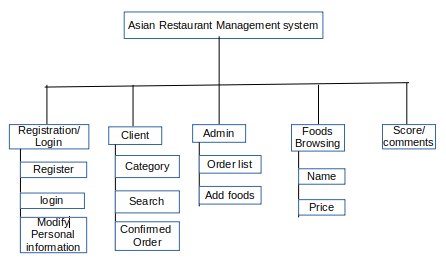
\includegraphics[height=3in]{/home/basedul/Documents/Report-writing-using-latex/ResturentManagementSystemReport/archtecturaldesign.png}
		\caption{System block diagram.}
		\label{fig:archi} 
	\end{figure}
		
	\tab As show on figure\ref{fig:archi} is showing the \textbf{Asian Restaurant Management System} is divided into some modules and submodules.
\subsection{Database Diagram}
	\subsubsection{Entity Diagram}
	\tab These diagrams below show how the attributes are defined in database table:\\
	
	\vspace{0.7cm}
	\tab An admin who must entry his personal information like first name, last name, user name, email and password.
	\begin{figure}[H]
		\centering
		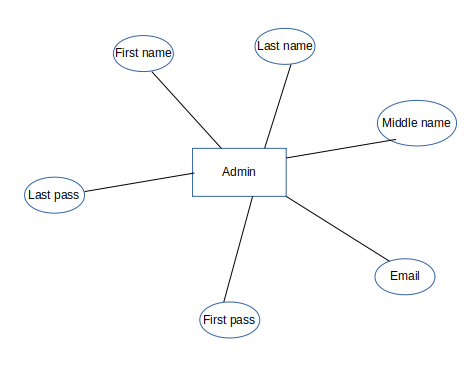
\includegraphics[height=3in]{/home/basedul/Documents/Report-writing-using-latex/ResturentManagementSystemReport/adminent.png}
		\caption{Admin Register entity diagram}
		\label{fig:adminreg} 
	\end{figure}
	\tab Client who must entry his personal information like first name, last name, user name, email and password.
	\begin{figure}[H]
		\centering
		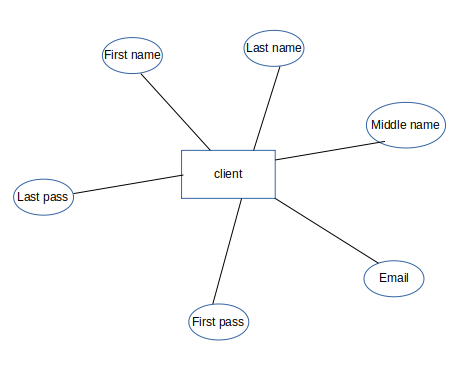
\includegraphics[height=3in]{/home/basedul/Documents/Report-writing-using-latex/ResturentManagementSystemReport/cliententy.png}
		\caption{Client Register entity diagram}
		\label{fig:clientreg} 
	\end{figure}
	
	\tab When add food on food list, must include food name, food price and details of food.
	\begin{figure}[H]
		\centering
		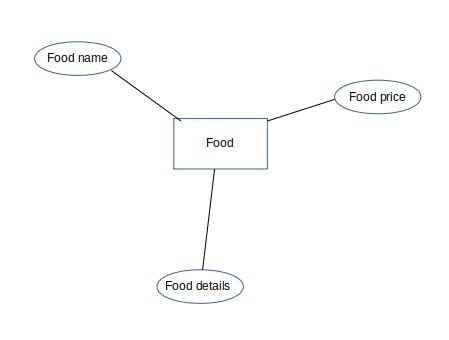
\includegraphics[height=3in]{/home/basedul/Documents/Report-writing-using-latex/ResturentManagementSystemReport/fooddet.png}
		\caption{Food add entity diagram}
		\label{fig:foodadd} 
	\end{figure}
	
	\tab When a client post his comment, client must be give name of food and select the score number.
	\begin{figure}[H]
		\centering
		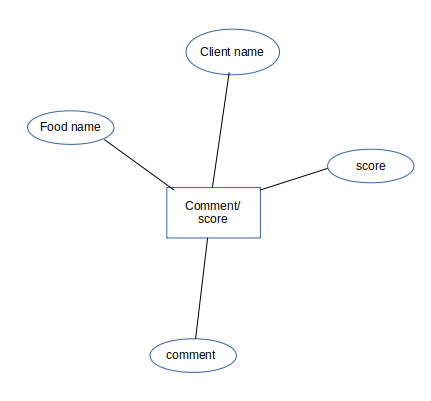
\includegraphics[height=3in]{/home/basedul/Documents/Report-writing-using-latex/ResturentManagementSystemReport/commtent.png}
		\caption{Comments/Score entity diagram}
		\label{fig:commentsent} 
	\end{figure}
	
	\subsubsection{E-R Diagram}
		\begin{figure}[H]
		\centering
		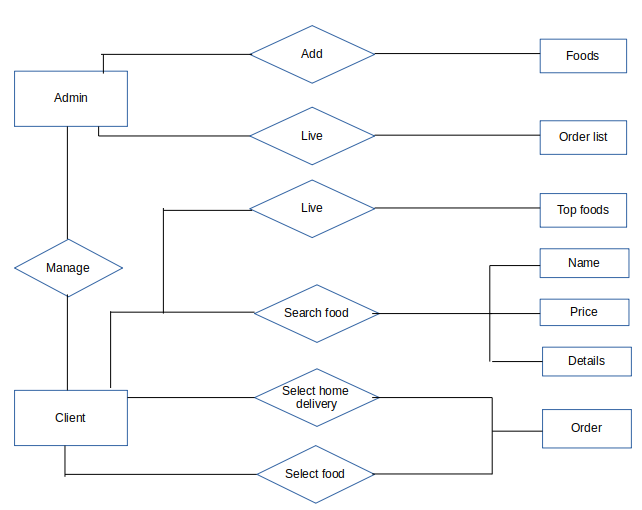
\includegraphics[height=3in]{/home/basedul/Documents/Report-writing-using-latex/ResturentManagementSystemReport/erdiag.png}
		\caption{Entity Relationship diagram}
		\label{fig:erdig} 
	\end{figure}
	
	\subsubsection{Database schema}
%			RegistrationForAdmin(uid, uf, ul, uu, um, ufp, usp, status)\\
%			Registration(uid, uf, ul, uu, um, ufp, usp, status)\\
%			APPTIZERS(appid, appname, appprice, appdetails)\\
%			BeefLamb(blid, blname, blprice, bldetails)\\
%			Chicken(ckid, ckname, ckprice, ckdetails)\\
%			Drink(did, dname, dprice, ddetails)\\
%			NoddlesRice(nrid, nrname, nrprice, nrdetails)\\
%			Pork(poid, poname, poprice, podetails)\\
%			Salad(said, saname, saprice, sadetails)\\
%			SeaFood(sfid, sfname, sfprice, sfdetails)\\
%			Soups(soid, soname, soprice, sodetails)\\
%			VegeTofu(vtid, vtname, vtprice, vtdetails)\\
%			ClientOrderList(colid, colname, colprice, colUser)\\
%			RankList(rlid, rlname, rlscore, rlcomments)
	
	
	
	\begin{lstlisting}[
           language=SQL,
           showspaces=false,
           basicstyle=\ttfamily,
           %numbers=left,
           numberstyle=\tiny,
           commentstyle=\color{gray}
        ]
		1. Create database ResturentManagement;
		
		2. CREATE TABLE RegistrationForAdmin (
		u_id TINYINT UNSIGNED NOT NULL AUTO_INCREMENT,
		u_f_name varchar(80),
		u_l_name varchar(80),
		u_u_name varchar(80),
		U_mail varchar(50),
		u_f_pass varchar(20),
		u_r_pass varchar(20),
		status int(11)
		PRIMARY KEY (u_id)
		)ENGINE=InnoDB DEFAULT CHARSET=utf8;
		
		3. CREATE TABLE Salad (
		sl_id TINYINT UNSIGNED NOT NULL AUTO_INCREMENT,
		sl_name varchar(255),
		sl_price float(10, 2),
		sl_details varchar(255),
		PRIMARY KEY (sl_id)
		)ENGINE=InnoDB DEFAULT CHARSET=utf8;

 		4. CREATE TABLE Soups (
		so_id TINYINT UNSIGNED NOT NULL AUTO_INCREMENT,
		so_name varchar(255),
		so_price float(10, 2),
		so_details varchar(255),
		PRIMARY KEY (so_id)
		)ENGINE=InnoDB DEFAULT CHARSET=utf8;

  		5. CREATE TABLE Chicken (
		ck_id TINYINT UNSIGNED NOT NULL AUTO_INCREMENT,
		ck_name varchar(255),
		ck_price float(10, 2),
		ck_details varchar(255),
		PRIMARY KEY (ck_id)
		)ENGINE=InnoDB DEFAULT CHARSET=utf8;

		6. CREATE TABLE Pork (
		po_id TINYINT UNSIGNED NOT NULL AUTO_INCREMENT,
		po_name varchar(255),
		po_price float(10, 2),
		po_details varchar(255),
		PRIMARY KEY (po_id)
		)ENGINE=InnoDB DEFAULT CHARSET=utf8;

	 	7. CREATE TABLE BeefLamb (
		bl_id TINYINT UNSIGNED NOT NULL AUTO_INCREMENT,
		bl_name varchar(255),
		bl_price float(10, 2),
		bl_details varchar(255),
		PRIMARY KEY (bl_id)
		)ENGINE=InnoDB DEFAULT CHARSET=utf8;

		8. CREATE TABLE SeaFood (
		sf_id TINYINT UNSIGNED NOT NULL AUTO_INCREMENT,
		sf_name varchar(255),
		sf_price float(10, 2),
		sf_details varchar(255),
		PRIMARY KEY (sf_id)
		)ENGINE=InnoDB DEFAULT CHARSET=utf8;

	 	9. CREATE TABLE NoddlesRice (
		nr_id TINYINT UNSIGNED NOT NULL AUTO_INCREMENT,
		nr_name varchar(255),
		nr_price float(10, 2),
		nr_details varchar(255),
		PRIMARY KEY (nr_id)
		)ENGINE=InnoDB DEFAULT CHARSET=utf8;

	 	10. CREATE TABLE VegeTofu (
		vt_id TINYINT UNSIGNED NOT NULL AUTO_INCREMENT,
		vt_name varchar(255),
		vt_price float(10, 2),
		vt_details varchar(255),
		PRIMARY KEY (vt_id)
		)ENGINE=InnoDB DEFAULT CHARSET=utf8;

	 	11. CREATE TABLE ClientOrderList (
		col_id TINYINT UNSIGNED NOT NULL AUTO_INCREMENT,
		col_name varchar(255),
		col_price float(10, 2),
		UserName varchar(255),
		PRIMARY KEY (col_id)
		)ENGINE=InnoDB DEFAULT CHARSET=utf8;

	 	12. ALTER TABLE `ClientOrderList` ADD `UserName` VARCHAR(255) NOT NULL AFTER `col_price`;

	 	13. CREATE TABLE RankList (
		rl_id TINYINT UNSIGNED NOT NULL AUTO_INCREMENT,
		rl_name varchar(255),
		rl_score int,
		rl_comments varchar(255),
		PRIMARY KEY (rl_id)
		)ENGINE=InnoDB DEFAULT CHARSET=utf8;
		
	 	14. ALTER TABLE `Registration` ADD `reward_point` float(10, 2) NOT NULL AFTER `status`;
		
	\end{lstlisting}
	
	\subsubsection{Database tables structures}
		\tab The table \ref{tab:adminregitable} is used for register a user as a admin of the system.
		\begin{table}[H]
		\center
	\caption{Registration for admin}
	\label{tab:adminregitable}
	\begin{tabular}{|M{2.5cm}|M{3.5cm}|M{1cm}|N}
	\hline
	\fontsize{10}{5}\fontfamily{ptm}\selectfont {\bfseries{Name}} & \fontsize{10}{5}\fontfamily{ptm}\selectfont {\bfseries{Type}} & \fontsize{10}{5}\fontfamily{ptm}\selectfont {\bfseries{Null}} &\\[10pt]
	\hline
	\fontsize{10}{5}\fontfamily{ptm}\selectfont {u-id} & \fontsize{10}{5}\fontfamily{ptm}\selectfont {tinyint(3)} & \fontsize{10}{5}\fontfamily{ptm}\selectfont {NO} &\\[10pt]
	\hline
	\fontsize{10}{5}\fontfamily{ptm}\selectfont {u-f-name} & \fontsize{10}{5}\fontfamily{ptm}\selectfont {varchar(80)} & \fontsize{10}{5}\fontfamily{ptm}\selectfont {YES} &\\[10pt]
	\hline
	\fontsize{10}{5}\fontfamily{ptm}\selectfont {u-l-name} & \fontsize{10}{5}\fontfamily{ptm}\selectfont {varchar(80)} & \fontsize{10}{5}\fontfamily{ptm}\selectfont {YES} &\\[10pt]
	\hline
	\fontsize{10}{5}\fontfamily{ptm}\selectfont {u-u-name} & \fontsize{10}{5}\fontfamily{ptm}\selectfont {varchar(80)} & \fontsize{10}{5}\fontfamily{ptm}\selectfont {YES} &\\[10pt]
	\hline
	\fontsize{10}{5}\fontfamily{ptm}\selectfont {U-mail} & \fontsize{10}{5}\fontfamily{ptm}\selectfont {varchar(50)} & \fontsize{10}{5}\fontfamily{ptm}\selectfont {YES} &\\[10pt]
	\hline
	\fontsize{10}{5}\fontfamily{ptm}\selectfont {u-f-pass} & \fontsize{10}{5}\fontfamily{ptm}\selectfont {varchar(20)} & \fontsize{10}{5}\fontfamily{ptm}\selectfont {YES} &\\[10pt]
	\hline
	\fontsize{10}{5}\fontfamily{ptm}\selectfont {u-l-pass} & \fontsize{10}{5}\fontfamily{ptm}\selectfont {varchar(20)} & \fontsize{10}{5}\fontfamily{ptm}\selectfont {YES} &\\[10pt]
	\hline
	\end{tabular}
	\end{table}
	\tab The table \ref{tab:clientregitable} is used for register a user as a client of the system.
	\begin{table}[H]
		\center
	\caption{Registration for client}
	\label{tab:clientregitable}
	\begin{tabular}{|M{2.5cm}|M{3.5cm}|M{1cm}|N}
	\hline
	\fontsize{10}{5}\fontfamily{ptm}\selectfont {\bfseries{Name}} & \fontsize{10}{5}\fontfamily{ptm}\selectfont {\bfseries{Type}} & \fontsize{10}{5}\fontfamily{ptm}\selectfont {\bfseries{Null}} &\\[10pt]
	\hline
	\fontsize{10}{5}\fontfamily{ptm}\selectfont {u-id} & \fontsize{10}{5}\fontfamily{ptm}\selectfont {tinyint(3)} & \fontsize{10}{5}\fontfamily{ptm}\selectfont {NO} &\\[10pt]
	\hline
	\fontsize{10}{5}\fontfamily{ptm}\selectfont {u-f-name} & \fontsize{10}{5}\fontfamily{ptm}\selectfont {varchar(80)} & \fontsize{10}{5}\fontfamily{ptm}\selectfont {YES} &\\[10pt]
	\hline
	\fontsize{10}{5}\fontfamily{ptm}\selectfont {u-l-name} & \fontsize{10}{5}\fontfamily{ptm}\selectfont {varchar(80)} & \fontsize{10}{5}\fontfamily{ptm}\selectfont {YES} &\\[10pt]
	\hline
	\fontsize{10}{5}\fontfamily{ptm}\selectfont {u-u-name} & \fontsize{10}{5}\fontfamily{ptm}\selectfont {varchar(80)} & \fontsize{10}{5}\fontfamily{ptm}\selectfont {YES} &\\[10pt]
	\hline
	\fontsize{10}{5}\fontfamily{ptm}\selectfont {U-mail} & \fontsize{10}{5}\fontfamily{ptm}\selectfont {varchar(50)} & \fontsize{10}{5}\fontfamily{ptm}\selectfont {YES} &\\[10pt]
	\hline
	\fontsize{10}{5}\fontfamily{ptm}\selectfont {u-f-pass} & \fontsize{10}{5}\fontfamily{ptm}\selectfont {varchar(20)} & \fontsize{10}{5}\fontfamily{ptm}\selectfont {YES} &\\[10pt]
	\hline
	\fontsize{10}{5}\fontfamily{ptm}\selectfont {u-l-pass} & \fontsize{10}{5}\fontfamily{ptm}\selectfont {varchar(20)} & \fontsize{10}{5}\fontfamily{ptm}\selectfont {YES} &\\[10pt]
	\hline
	\end{tabular}
	\end{table}
	
	\tab The table \ref{tab:clientorderlist} is used for hold the list of chooseing foods by client 
	\begin{table}[H]
		\center
	\caption{Client order list}
	\label{tab:clientorderlist}
	\begin{tabular}{|M{2.5cm}|M{3.5cm}|M{1cm}|N}
	\hline
	\fontsize{10}{5}\fontfamily{ptm}\selectfont {\bfseries{Name}} & \fontsize{10}{5}\fontfamily{ptm}\selectfont {\bfseries{Type}} & \fontsize{10}{5}\fontfamily{ptm}\selectfont {\bfseries{Null}} &\\[10pt]
	\hline
	\fontsize{10}{5}\fontfamily{ptm}\selectfont {col-id} & \fontsize{10}{5}\fontfamily{ptm}\selectfont {tinyint(3)} & \fontsize{10}{5}\fontfamily{ptm}\selectfont {NO} &\\[10pt]
	\hline
	\fontsize{10}{5}\fontfamily{ptm}\selectfont {col-name} & \fontsize{10}{5}\fontfamily{ptm}\selectfont {varchar(255)} & \fontsize{10}{5}\fontfamily{ptm}\selectfont {YES} &\\[10pt]
	\hline
	\fontsize{10}{5}\fontfamily{ptm}\selectfont {col-price} & \fontsize{10}{5}\fontfamily{ptm}\selectfont {float(10, 2)} & \fontsize{10}{5}\fontfamily{ptm}\selectfont {YES} &\\[10pt]
	\hline
	\fontsize{10}{5}\fontfamily{ptm}\selectfont {UserName} & \fontsize{10}{5}\fontfamily{ptm}\selectfont {varchar(255)} & \fontsize{10}{5}\fontfamily{ptm}\selectfont {YES} &\\[10pt]
	\hline
	
	\end{tabular}
	\end{table}
	
	\tab This table \ref{tab:topfoods} is used for hold the list of top ranked food depend on score number and number of comments.
	\begin{table}[H]
		\center
	\caption{Top foods}
	\label{tab:topfoods}
	\begin{tabular}{|M{2.5cm}|M{3.5cm}|M{1cm}|N}
	\hline
	\fontsize{10}{5}\fontfamily{ptm}\selectfont {\bfseries{Name}} & \fontsize{10}{5}\fontfamily{ptm}\selectfont {\bfseries{Type}} & \fontsize{10}{5}\fontfamily{ptm}\selectfont {\bfseries{Null}} &\\[10pt]
	\hline
	\fontsize{10}{5}\fontfamily{ptm}\selectfont {dl-id} & \fontsize{10}{5}\fontfamily{ptm}\selectfont {tinyint(3)} & \fontsize{10}{5}\fontfamily{ptm}\selectfont {NO} &\\[10pt]
	\hline
	\fontsize{10}{5}\fontfamily{ptm}\selectfont {rl-name} & \fontsize{10}{5}\fontfamily{ptm}\selectfont {varchar(255)} & \fontsize{10}{5}\fontfamily{ptm}\selectfont {YES} &\\[10pt]
	\hline
	\fontsize{10}{5}\fontfamily{ptm}\selectfont {rl-score} & \fontsize{10}{5}\fontfamily{ptm}\selectfont {int} & \fontsize{10}{5}\fontfamily{ptm}\selectfont {YES} &\\[10pt]
	\hline
	\fontsize{10}{5}\fontfamily{ptm}\selectfont {rl-comments} & \fontsize{10}{5}\fontfamily{ptm}\selectfont {varchar(255)} & \fontsize{10}{5}\fontfamily{ptm}\selectfont {YES} &\\[10pt]
	\hline
	\end{tabular}
	\end{table}
	
	\tab This table \ref{tab:salad} is used for hold the list of salads.
	\begin{table}[H]
		\center
	\caption{Salad table}
	\label{tab:salad}
	\begin{tabular}{|M{2.5cm}|M{3.5cm}|M{1cm}|N}
	\hline
	\fontsize{10}{5}\fontfamily{ptm}\selectfont {\bfseries{Name}} & \fontsize{10}{5}\fontfamily{ptm}\selectfont {\bfseries{Type}} & \fontsize{10}{5}\fontfamily{ptm}\selectfont {\bfseries{Null}} &\\[10pt]
	\hline
	\fontsize{10}{5}\fontfamily{ptm}\selectfont {sl-id} & \fontsize{10}{5}\fontfamily{ptm}\selectfont {tinyint(3)} & \fontsize{10}{5}\fontfamily{ptm}\selectfont {NO} &\\[10pt]
	\hline
	\fontsize{10}{5}\fontfamily{ptm}\selectfont {sl-name} & \fontsize{10}{5}\fontfamily{ptm}\selectfont {varchar(255)} & \fontsize{10}{5}\fontfamily{ptm}\selectfont {YES} &\\[10pt]
	\hline
	\fontsize{10}{5}\fontfamily{ptm}\selectfont {sl-price} & \fontsize{10}{5}\fontfamily{ptm}\selectfont {float(10, 2)} & \fontsize{10}{5}\fontfamily{ptm}\selectfont {YES} &\\[10pt]
	\hline
	\fontsize{10}{5}\fontfamily{ptm}\selectfont {sl-details} & \fontsize{10}{5}\fontfamily{ptm}\selectfont {varchar(255)} & \fontsize{10}{5}\fontfamily{ptm}\selectfont {YES} &\\[10pt]
	\hline
	\end{tabular}
	\end{table}
	
	\tab This table \ref{tab:chicken} is used for hold the list of Chickens.
	\begin{table}[H]
		\center
	\caption{Chicken table}
	\label{tab:chicken}
	\begin{tabular}{|M{2.5cm}|M{3.5cm}|M{1cm}|N}
	\hline
	\fontsize{10}{5}\fontfamily{ptm}\selectfont {\bfseries{Name}} & \fontsize{10}{5}\fontfamily{ptm}\selectfont {\bfseries{Type}} & \fontsize{10}{5}\fontfamily{ptm}\selectfont {\bfseries{Null}} &\\[10pt]
	\hline
	\fontsize{10}{5}\fontfamily{ptm}\selectfont {ck-id} & \fontsize{10}{5}\fontfamily{ptm}\selectfont {tinyint(3)} & \fontsize{10}{5}\fontfamily{ptm}\selectfont {NO} &\\[10pt]
	\hline
	\fontsize{10}{5}\fontfamily{ptm}\selectfont {ck-name} & \fontsize{10}{5}\fontfamily{ptm}\selectfont {varchar(255)} & \fontsize{10}{5}\fontfamily{ptm}\selectfont {YES} &\\[10pt]
	\hline
	\fontsize{10}{5}\fontfamily{ptm}\selectfont {ck-price} & \fontsize{10}{5}\fontfamily{ptm}\selectfont {float(10, 2)} & \fontsize{10}{5}\fontfamily{ptm}\selectfont {YES} &\\[10pt]
	\hline
	\fontsize{10}{5}\fontfamily{ptm}\selectfont {ck-details} & \fontsize{10}{5}\fontfamily{ptm}\selectfont {varchar(255)} & \fontsize{10}{5}\fontfamily{ptm}\selectfont {YES} &\\[10pt]
	\hline
	\end{tabular}
	\end{table}
	
	\tab This table \ref{tab:vegetofu} is used for hold the list of Vegetables and Tofus.
	\begin{table}[H]
		\center
	\caption{Vegetable and Tofu table}
	\label{tab:vegetofu}
	\begin{tabular}{|M{2.5cm}|M{3.5cm}|M{1cm}|N}
	\hline
	\fontsize{10}{5}\fontfamily{ptm}\selectfont {\bfseries{Name}} & \fontsize{10}{5}\fontfamily{ptm}\selectfont {\bfseries{Type}} & \fontsize{10}{5}\fontfamily{ptm}\selectfont {\bfseries{Null}} &\\[10pt]
	\hline
	\fontsize{10}{5}\fontfamily{ptm}\selectfont {vt-id} & \fontsize{10}{5}\fontfamily{ptm}\selectfont {tinyint(3)} & \fontsize{10}{5}\fontfamily{ptm}\selectfont {NO} &\\[10pt]
	\hline
	\fontsize{10}{5}\fontfamily{ptm}\selectfont {vt-name} & \fontsize{10}{5}\fontfamily{ptm}\selectfont {varchar(255)} & \fontsize{10}{5}\fontfamily{ptm}\selectfont {YES} &\\[10pt]
	\hline
	\fontsize{10}{5}\fontfamily{ptm}\selectfont {vt-price} & \fontsize{10}{5}\fontfamily{ptm}\selectfont {float(10, 2)} & \fontsize{10}{5}\fontfamily{ptm}\selectfont {YES} &\\[10pt]
	\hline
	\fontsize{10}{5}\fontfamily{ptm}\selectfont {vt-details} & \fontsize{10}{5}\fontfamily{ptm}\selectfont {varchar(255)} & \fontsize{10}{5}\fontfamily{ptm}\selectfont {YES} &\\[10pt]
	\hline
	\end{tabular}
	\end{table}
	
	\tab This table \ref{tab:nodrice} is used for hold the list of Noodles and Rice.
	\begin{table}[H]
		\center
	\caption{Noodles and Rice table}
	\label{tab:nodrice}
	\begin{tabular}{|M{2.5cm}|M{3.5cm}|M{1cm}|N}
	\hline
	\fontsize{10}{5}\fontfamily{ptm}\selectfont {\bfseries{Name}} & \fontsize{10}{5}\fontfamily{ptm}\selectfont {\bfseries{Type}} & \fontsize{10}{5}\fontfamily{ptm}\selectfont {\bfseries{Null}} &\\[10pt]
	\hline
	\fontsize{10}{5}\fontfamily{ptm}\selectfont {nr-id} & \fontsize{10}{5}\fontfamily{ptm}\selectfont {tinyint(3)} & \fontsize{10}{5}\fontfamily{ptm}\selectfont {NO} &\\[10pt]
	\hline
	\fontsize{10}{5}\fontfamily{ptm}\selectfont {nr-name} & \fontsize{10}{5}\fontfamily{ptm}\selectfont {varchar(255)} & \fontsize{10}{5}\fontfamily{ptm}\selectfont {YES} &\\[10pt]
	\hline
	\fontsize{10}{5}\fontfamily{ptm}\selectfont {nr-price} & \fontsize{10}{5}\fontfamily{ptm}\selectfont {float(10, 2)} & \fontsize{10}{5}\fontfamily{ptm}\selectfont {YES} &\\[10pt]
	\hline
	\fontsize{10}{5}\fontfamily{ptm}\selectfont {nr-details} & \fontsize{10}{5}\fontfamily{ptm}\selectfont {varchar(255)} & \fontsize{10}{5}\fontfamily{ptm}\selectfont {YES} &\\[10pt]
	\hline
	\end{tabular}
	\end{table}
	
	
	
\newpage

\section{Design}
%{\bfseries\Large Design}
	\subsection{Chapter Overview}
	\tab This chapter will focus on the design of the system using diagrams to illustrate graphically certain
sections of the software system.

	\subsection{Detailed Design}
	\tab In this section, I designed the first flowchart of the Asian Restaurant Management System. The purpose
of the flowchart is to show functions the Asian Restaurant Management System has.	
	
		\begin{figure}[H]
		\centering
		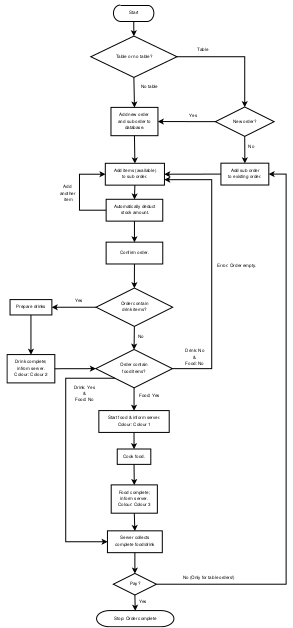
\includegraphics[height=3.2in]{/home/basedul/Documents/Report-writing-using-latex/ResturentManagementSystemReport/flowchart.png}
		\caption{System flowchart}
		\label{fig:flowchart} 
	\end{figure}
	\subsection{Manager and Customer function}
	\subsubsection{Register or login function}
	\tab Every time a registered user is must to login in order to client confirmed order or admin see the order list or new food add on table, the
user has to input both of the correct user name and the password into the input-form. The
application will get the input data and send to the system Server, and the server will
communicate with the MySQL database and check if the user name and password are	matched. If the input is correct, the the order of clent will display the main window with the
name of the user. Otherwise, the error-
window will be instead.
		\begin{figure}[H]
		\centering
		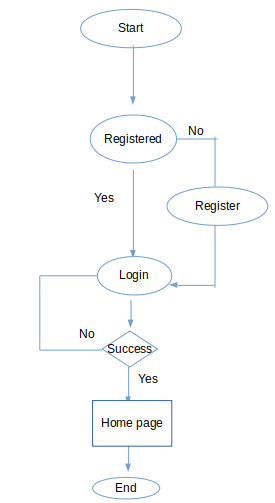
\includegraphics[height=6in]{/home/basedul/Documents/Report-writing-using-latex/ResturentManagementSystemReport/regispag.png}
		\caption{Registration flowchart}
		\label{fig:regiflow} 
		\end{figure}
	
	\subsubsection{Order list}
		\tab After successfully admin login, he/she see the list of order.
		\begin{figure}[H]
		\centering
		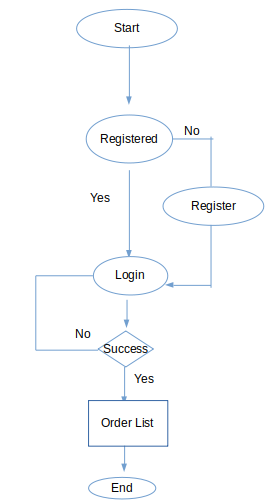
\includegraphics[height=6in]{/home/basedul/Documents/Report-writing-using-latex/ResturentManagementSystemReport/seeclientorderlist.png}
		\caption{Client order list flowchart}
		\label{fig:seeclientorderlist} 
		\end{figure}
		
	\subsubsection{Confirmed order after successfull signin}
		\tab After successfully client login, he/she confirmed the order.
		\begin{figure}[H]
		\centering
		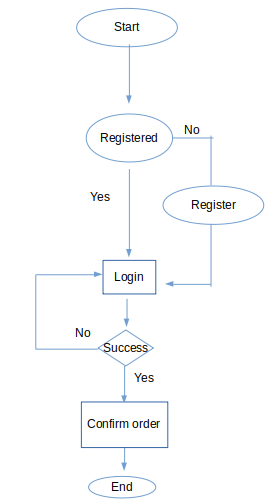
\includegraphics[height=6in]{/home/basedul/Documents/Report-writing-using-latex/ResturentManagementSystemReport/confirmedOrder.png}
		\caption{Confirmed order flowchart}
		\label{fig:confirmedOrder} 
		\end{figure}
		

		
		
		
	\begin{comment}		
		
	\begin{comment}
	\subsection{Introduction}
	\tab This project has been designed using numerous diagrammatic techniques. Recall from Section \ref{fig:uml}, that
the most general modelling language to describe both the structure and behaviour of a software system
is Unified Modelling language (UML).
Use case diagrams have already been used in the requirements analysis as a way to graphically
overview the order process within the system. Other diagrams from the UML family are used in the
design stage to show the structure and behaviour of numerous sophisticated design feature.
\subsection{Component Diagram}
\tab A component diagram is part of UML and its main purpose is to show the structural relationship
between components in the system. A component diagram is useful for this system as it shows the
higher architecture, as shown in figure \ref{fig:comdia}
\begin{figure}[H]
		\centering
		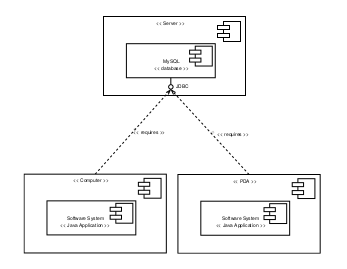
\includegraphics[height=3in]{/home/basedul/Documents/Report-writing-using-latex/ResturentManagementSystemReport/comdia.png}
		\caption{Component diagram showing the higher level architecture of the system.}
		\label{fig:comdia} 
	\end{figure}
	
\subsection{Data Storage}
	The restaurant management system will be built around the data storage technique therefore choosing
the most appropriate persistent 1 data storage is critical to a successful project and we can assume a flat
file storage approach is inadequate. The two most popular types of persistent data storage available
are relational database management system (RDBMS) and extensible markup language (XML)
\subsubsection{Relational Database Management System (RDBMS)}
	\label{Rel:RDBMS}
	A relational database management system (RDBMS) is a database managed system based around a
relational model and are the corner stone’s to many software systems including web based systems.\\
RDBMS are one of the most popular data storage methods out in the market and offer many advantages
including:\\
\begin{itemize}
	\item Fast data extraction using structured query language (SQL).
	\item Good management of data and security through the management system.
	\item Good level of data consistency.
	\item Advanced features including functions and triggers.
	\item Requirement of a data model to be developed; leading to long term cost effectiveness. 
\end{itemize}
In industry, there are numerous expensive highly functional RDMBSs including Oracle and SQLServer
that are very popular and offer technical support. However, there are also numerous open-source solu-
tions with many adjudged to be as good or better and are becoming even more popular with small
scale software systems.
\subsubsection{Extensible Markup Language (XML)}
	XML is a markup language that was designed to transport and store data and is another example of
a persistent data storage technique. However, it is not a predefined language thus all tags must be
defined and due to its hierarchically data structure all elements must be promoted or demoted.
XML could be used in two different ways in data storage; storing the XML documents within a
database or having the XML documents as the fundamental unit of storage. In both cases the XML
can be queried using either XPATH or XQUERY which are query languages for extracting data from
XML documents.
\subsubsection{Storage Method Chosen}
	The main difference between XML and RDBMS is that XML is hierarchical and RDBMS is relational.
As restaurant data can be best represented in a hierarchical way one would believe that XML would be
the best approach but it’s not always that straight forward. SQL is an extremely flexible and robust querying language and for the queries required and the type of software system begin designed, it was
concluded that RDBMS would be the best storage method.
The next choice was to decide on the type of RDBMS to use. As discussed there are many open
source RDBMSs available for us to choose from and for the main reason of experience, MySQL was the
preferred option. Figure \ref{fig:compari} shows just how competitive the performances of different RDBMSs are.
\begin{figure}[H]
		\centering
		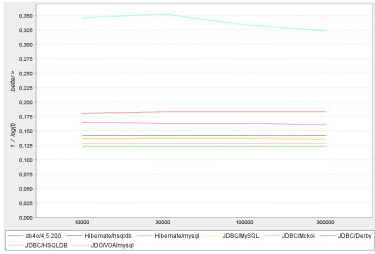
\includegraphics[height=4in]{/home/basedul/Documents/Report-writing-using-latex/ResturentManagementSystemReport/compari.png}
		\caption{Database comparison diagram \cite{Ref:6}}
		\label{fig:compari} 
	\end{figure}
\subsubsection{Normalisation}
Normalisation comes in many forms ranging from first normal form to sixth normal form. The nor-
malisation of a database is a systematic way to free the database of undesirable characteristics where
inserts, updates and deletions of data could lead to the loss of data integrity. The greater the normal
form, the greater the data integrity of the database.\\
The database in this system was designed to be in Boyce-Codd normal form which is a slightly
stronger version of the third normal form. For the database to be in Boyce-Codd normal form, it had
to pass for all previous normal forms as well as Boyce-Codd normal form.\\
A well designed database will normally abide by the first, second and third normal forms as they
are the basics to a well structured relational database. According to Horsforth School [17], the first
three normal forms can be defined as:
\begin{itemize}
	\item Every attribute is atomic or single valued therefore there are no repeating fields.
	\item All attributes not part of the primary key must be dependent on the full key.
	\item There must be no transitive determinants, or each attribute that is not part of
the key must be determined only by the key.
\end{itemize}
Finally for the database to be in the desired Boyce-Codd normal form, all tables must abide by the
first, second and third normal forms and must not have any determinants that are not candidate keys
for the table.
\end{commment}
\begin{comment}
\subsubsection{Entity Relationship Diagram}
	\label{sec:entity}
An entity relationship (ER) diagram is a modelling language used to represent a type of semantic
data model of a system. The ER diagrams are often used to represent a relational database and its
requirements in a top-down fashion usually defined as the database schema. The database schema for
this database has been split into two ER diagrams (Figures \ref{fig:entityone} and \ref{fig:entitytwo}).
Figure \ref{fig:entityone} graphically shows the objects and their relationships that are contained within a meal.
The meal object will be made of at least two ingredients that can be either a normal ingredient or
a prepared ingredient. Note, a prepared ingredient is a collection of ingredients used to either group
commonly used ingredients or to group optional ingredients. Each ingredient will have a default and
manual measurement with the default measurement entered on input of the ingredient and the manual
measurement entered if the meal ingredient link requires a different amount.
Also, each ingredient will be part of a generic ingredient object as there are many ingredients that
are the same item but packaged in a different way at a different price. This allows the database to be in
Boyce-Codd normalised state. An example of this would be the drink Coca-Cola which can be bought
by bottle, can or draught, thus are the same item but packaged differently at a different price and
amount. Finally each ingredient and prepared ingredient can be part of a category allowing optional
ingredients to be interchanged with other ingredients in the same category.
Figure \ref{fig:entitytwo} graphically shows the relationships for the menu, order and offer objects. The menu
consists of a date time relationship that provides the intervals to when the menu is active and a menu
section relationship that contains the colour variables and items under that particular menu section.
The order consists of one to many suborders with the suborder consisting of one to many items.
The order stores all the ingredients within each item and also the replaced ingredient if that optional
ingredient was replaced.
The offer consists of a date time relationship that provides the intervals to when the offer is active
and a offer section relationship that contains the sets required by the offer.
\begin{figure}[H]
		\centering
		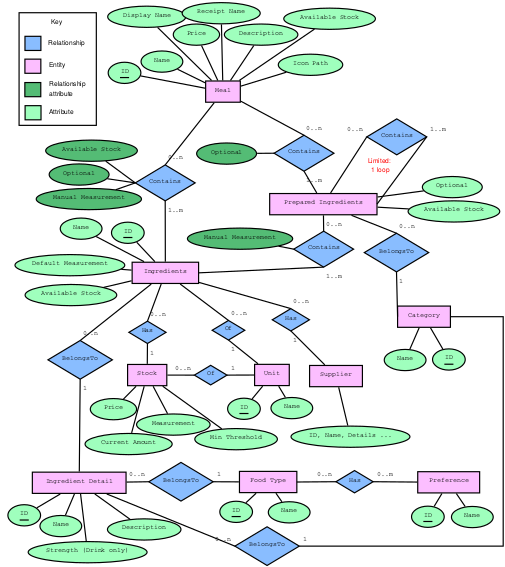
\includegraphics[height=6.5in]{/home/basedul/Documents/Report-writing-using-latex/ResturentManagementSystemReport/entityone.png}
		\caption{Entity Relationship diagram of a meal.}
		\label{fig:entityone} 
	\end{figure}
\begin{figure}[H]
		\centering
		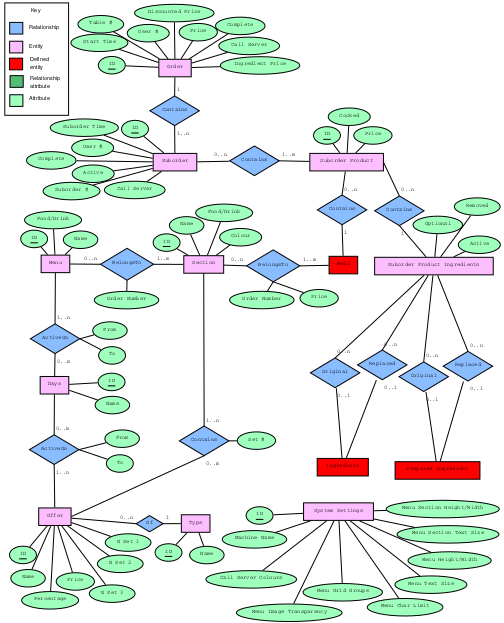
\includegraphics[height=6.5in]{/home/basedul/Documents/Report-writing-using-latex/ResturentManagementSystemReport/entitytwo.png}
		\caption{Entity Relationship of the menu, order and system settings.}
		\label{fig:entitytwo} 
	\end{figure}
	
\subsection{Graphical User Interface}	
\label{sec:guiinterface}
	The graphical user interface (GUI) is the only component of the system that the user interacts with
therefore is of great importance. The design had to be simple, clear and concise but whilst also showing
all of the required features. The main objective was to create a GUI that allowed the user to get the
order completed in the minimum time possible. This was judged by the time taken to complete the
order as well as the amount of clicks required to get from the start to the finish. In total, there are 2
different GUIs within the restaurant management system with each GUI requiring a different design
specification.
\subsubsection{Admin Gui}
The Admin system GUI has the most user interaction through the means of a touch screen. Hence
usability and user-friendliness of the GUI was of the highest priority. Therefore the specification was
as follows:\\
\begin{itemize}
	\item Chronological order of steps; either from left to right, top to bottom or a mixture of both.
	\item Minimum clicks from start to finish.
	\item Meal items.
	\item Ability to fit on any monitor size.
	\item Maximum space usage with readable font.
\end{itemize}
\begin{figure}[H]
		\centering
		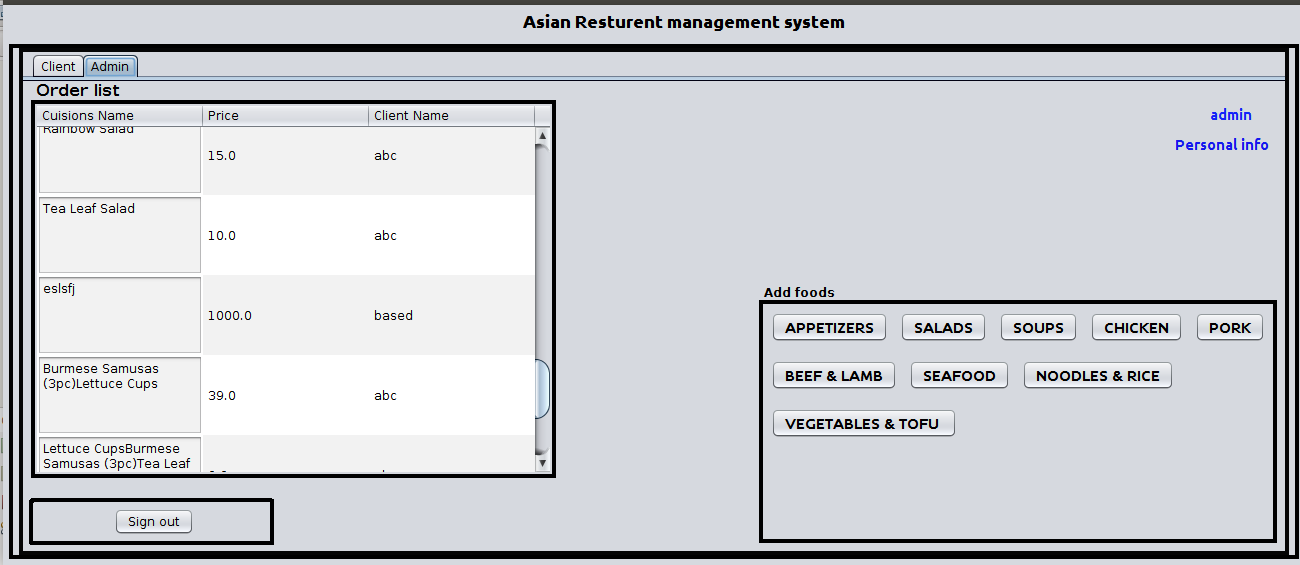
\includegraphics[height=3in]{/home/basedul/Documents/Report-writing-using-latex/ResturentManagementSystemReport/orderGui.png}
		\caption{Design of the Admin GUI for a monitor.}
		\label{fig:adminGui} 
\end{figure}
\subsubsection{Client Gui}
The Client system requires a GUI to input data therefore requires an appropriate input design.
Figure \ref{fig:clientGui} shows the design of the management application with the different functions appearing the left hand side as a tab. Each tab contains a subform with Figure 4.9 containing the structure
of the generic data input form.
\begin{figure}[H]
		\centering
		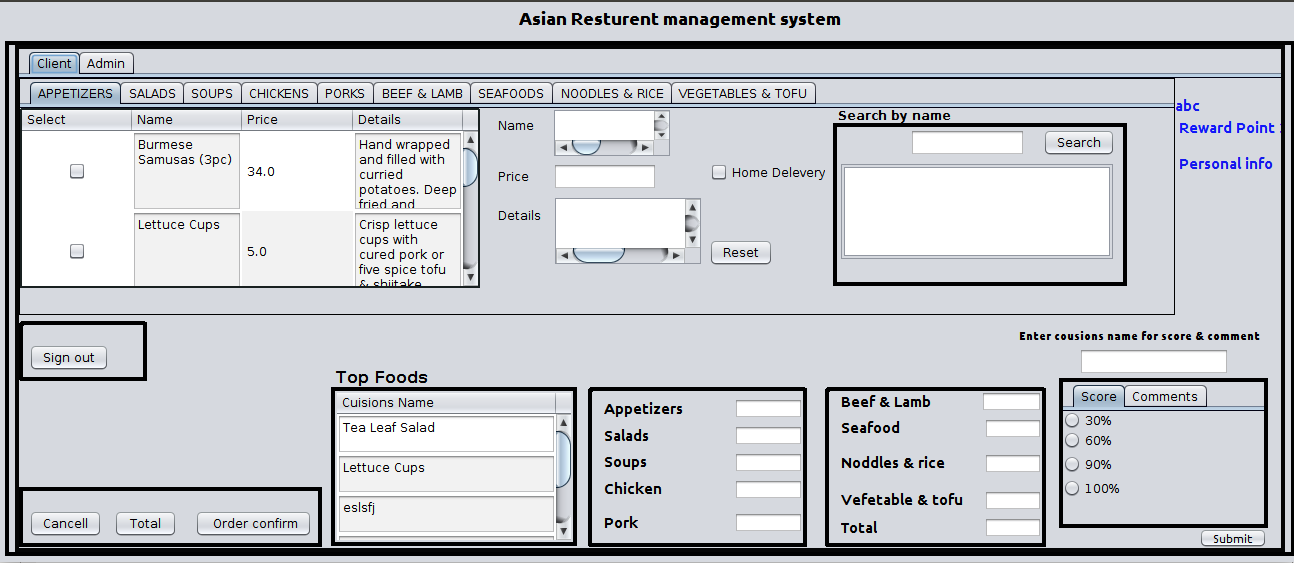
\includegraphics[height=3in]{/home/basedul/Documents/Report-writing-using-latex/ResturentManagementSystemReport/clientGui.png}
		\caption{Design of the Client GUI for a monitor.}
		\label{fig:clientGui} 
\end{figure}
	
\subsection{Flow Charts}
	A flow chart is a diagram used to represent the process flow of an algorithm, problem or some transaction
within a business. Therefore a flow chart (Figure \ref{fig:flowchart}) was used to graphically represent the process
flow of an order.
\begin{figure}[H]
		\centering
		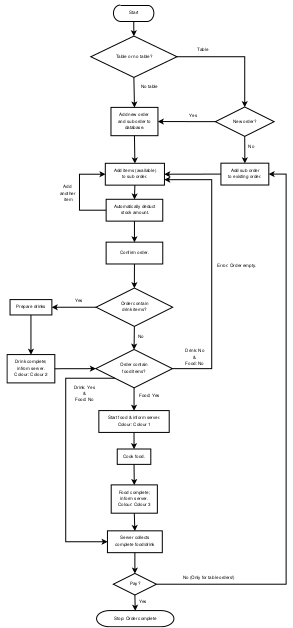
\includegraphics[height=6.5in]{/home/basedul/Documents/Report-writing-using-latex/ResturentManagementSystemReport/flowchart.png}
		\caption{Flow chart to show the flow of events of an order..}
		\label{fig:flowchart} 
\end{figure}
\end{comment}

\subsection{Chapter Summary}
	\tab This chapter has displayed many graphical representations of the design of the system. The implementation of the system is documented in the next chapter.
\newpage
\section{Implementation And Testing}
%{\bfseries \Large Implementation and Testing}
	\subsection{Chapter Overview}
	\tab Implementation is the process in the project in which the existing design is changed into working system and is giving assurance confidence on the new system for the users that it will work correctly. It involves careful planning, checkout of the current system and it compulsion or constraints of design, implementation of methods to achieve the changeover, an evaluation of the changeover methods. Apart from it planning major tasks of arranging the implementation are educating and training of users. The more complex the system is being implemented the more involved will be the system analysis and the design efforts requires just for the implementation. The implementation process begins at preparing a plan for the implementation of the system.
	\subsection{Document List}
	
		\begin{table}[H]
		\center
	\caption{Document list}
	\label{tab:vegetofu}
	\begin{tabular}{|M{0.7cm}|M{6cm}|M{9cm}|N}
	\hline
	\fontsize{10}{5}\fontfamily{ptm}\selectfont {\bfseries{No}} & \fontsize{10}{5}\fontfamily{ptm}\selectfont {\bfseries{Package name}} & \fontsize{10}{5}\fontfamily{ptm}\selectfont {\bfseries{Purpose}} &\\[10pt]
	\hline
	\fontsize{10}{5}\fontfamily{ptm}\selectfont {1} & \fontsize{10}{5}\fontfamily{ptm}\selectfont {Database connection} & \fontsize{10}{5}\fontfamily{ptm}\selectfont {This package use for implementation of database connection with local host using jdbc driver} &\\[10pt]
	\hline
	\fontsize{10}{5}\fontfamily{ptm}\selectfont {2} & \fontsize{10}{5}\fontfamily{ptm}\selectfont {Food add on database} & \fontsize{10}{5}\fontfamily{ptm}\selectfont {This package use for add food name, price and details into specific table of food} &\\[10pt]
	\hline
	\fontsize{10}{5}\fontfamily{ptm}\selectfont {3} & \fontsize{10}{5}\fontfamily{ptm}\selectfont {Home activity} & \fontsize{10}{5}\fontfamily{ptm}\selectfont {Home activity package use for design and implementation of homepage} &\\[10pt]
	\hline
	\fontsize{10}{5}\fontfamily{ptm}\selectfont {4} & \fontsize{10}{5}\fontfamily{ptm}\selectfont {Order insert into orderlist table} & \fontsize{10}{5}\fontfamily{ptm}\selectfont {After confirmed order from customer, these order are insert into order list table using this package} &\\[10pt]
	\hline
	\fontsize{10}{5}\fontfamily{ptm}\selectfont {5} & \fontsize{10}{5}\fontfamily{ptm}\selectfont {Order insert into orderlist table} & \fontsize{10}{5}\fontfamily{ptm}\selectfont {After confirmed order from customer, these order are insert into order list table using this package} &\\[10pt]
	\hline
	\fontsize{10}{5}\fontfamily{ptm}\selectfont {6} & \fontsize{10}{5}\fontfamily{ptm}\selectfont {Personal info show} & \fontsize{10}{5}\fontfamily{ptm}\selectfont {This package use for personal information show on homepage} &\\[10pt]
	\hline
	\fontsize{10}{5}\fontfamily{ptm}\selectfont {7} & \fontsize{10}{5}\fontfamily{ptm}\selectfont {Read data from Database} & \fontsize{10}{5}\fontfamily{ptm}\selectfont {This package use for read data from database and set into table on home page} &\\[10pt]
	\hline
	\fontsize{10}{5}\fontfamily{ptm}\selectfont {8} & \fontsize{10}{5}\fontfamily{ptm}\selectfont {Registration} & \fontsize{10}{5}\fontfamily{ptm}\selectfont {This package use for registration purpose of admin and client} &\\[10pt]
	\hline
	\fontsize{10}{5}\fontfamily{ptm}\selectfont {9} & \fontsize{10}{5}\fontfamily{ptm}\selectfont {Search from database} & \fontsize{10}{5}\fontfamily{ptm}\selectfont {This package use for searching an item by name or price of food from database} &\\[10pt]
	\hline
	\end{tabular}
	\end{table}
	
	\subsection{User module}
		\subsubsection{Sign in}
			\tab Already registered user will have to login in the system by inputting username and password in order to enter the system. The screen shot is shown in Fig \ref{fig:login} 
			\begin{figure}[H]
		\centering
		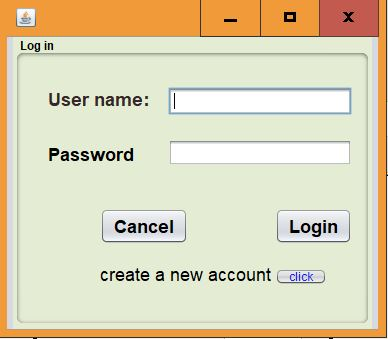
\includegraphics[height=2in]{/home/basedul/Documents/Report-writing-using-latex/ResturentManagementSystemReport/signin.JPG}
		\caption{Sign in window}
		\label{fig:login} 
		\end{figure}
		
		\subsubsection{Sign up}
			\tab A new user will have to sign up in the system by providing essential details in order to be a client of the restaurant. The screen shot is shown in Fig \ref{fig:log out} 
			\begin{figure}[H]
		\centering
		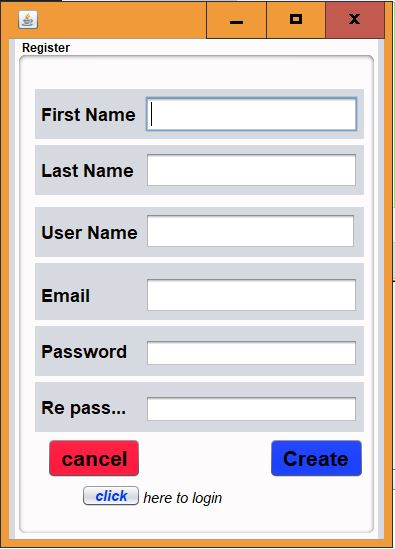
\includegraphics[height=3in]{/home/basedul/Documents/Report-writing-using-latex/ResturentManagementSystemReport/signup.JPG}
		\caption{Sign up window}
		\label{fig:log out} 
		\end{figure}
		
		\subsubsection{HomePage}
			\tab After a successful sign in, the client is redirected to the home activity of the application.  It includes the activities that happens in the restaurant and rewards  top foods also modifying about the personal information. The screen shot is shown in Fig \ref{fig:homepage} and Fig \ref{fig:topfood1}.
			\begin{figure}[H]
		\centering
		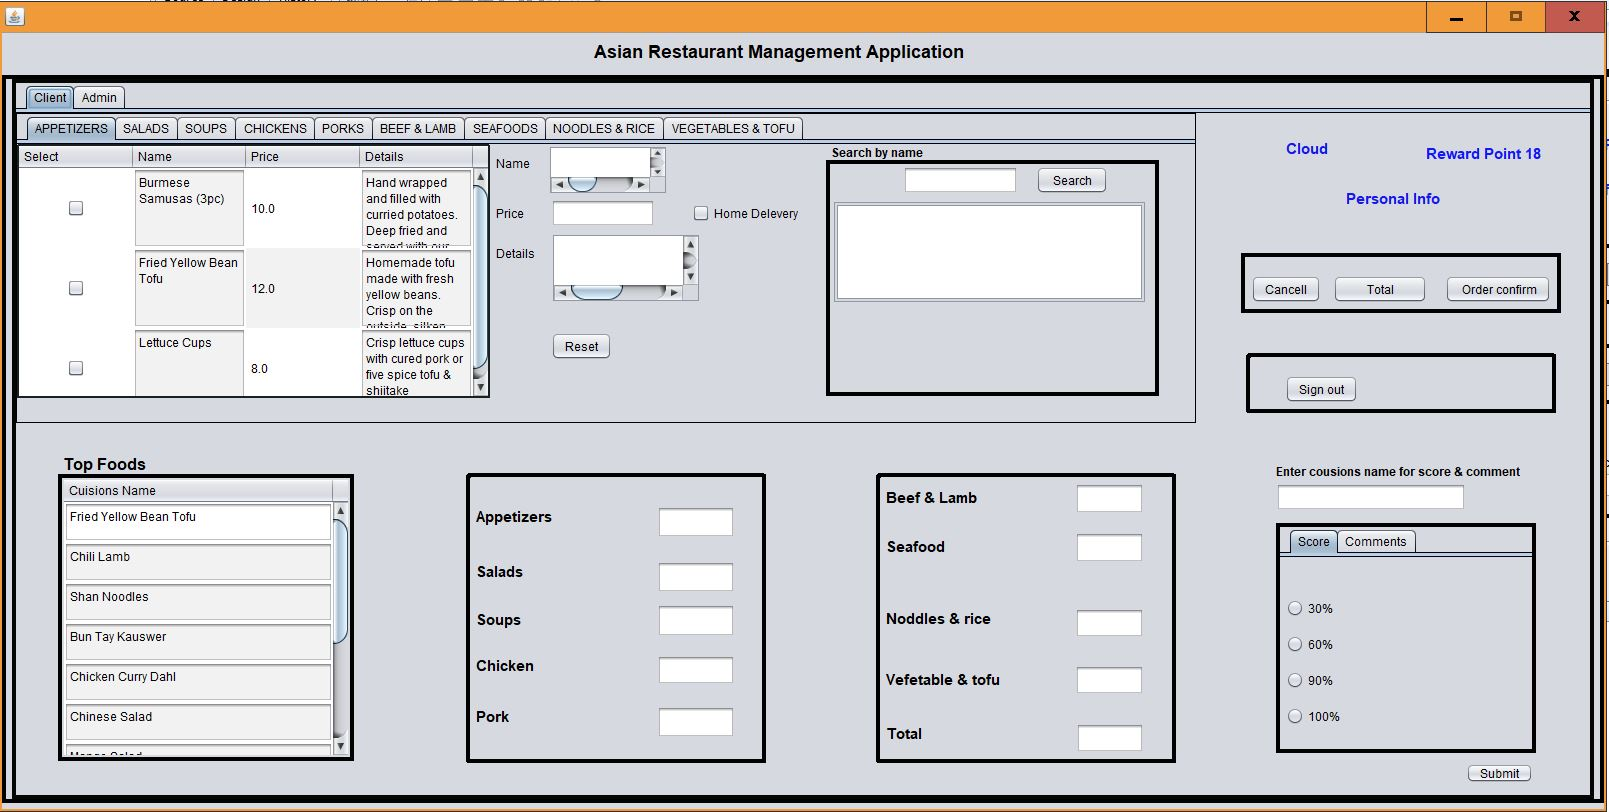
\includegraphics[height=2.3in]{/home/basedul/Documents/Report-writing-using-latex/ResturentManagementSystemReport/mainactivity.JPG}
		\caption{Homepage window}
		\label{fig:homepage} 
		
		
		\vspace{2cm}
		
		
		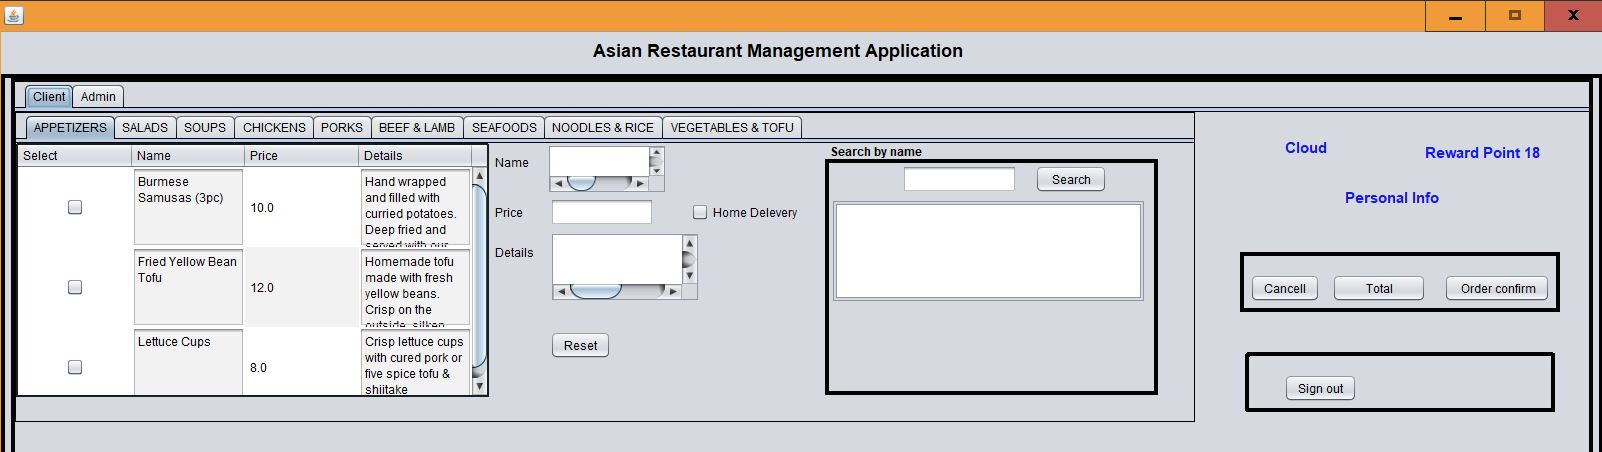
\includegraphics[height=1.7in]{/home/basedul/Documents/Report-writing-using-latex/ResturentManagementSystemReport/order.JPG}
		\caption{Order list window}
		\label{fig:topfood1} 	
		
		
		\end{figure}
		
		\subsubsection{Topfoods}
			\tab Write user experience or comment on the dish and submit satisfaction score and user get reward points after sharing their experiences. The screen shot is shown in Fig \ref{fig:topfood}. 
			\begin{figure}[H]
		\centering
		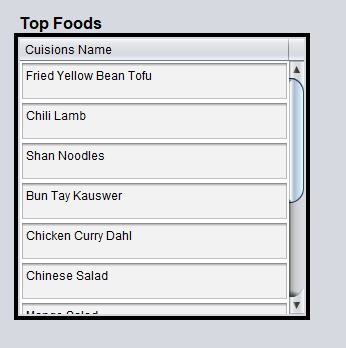
\includegraphics[height=2.3in]{/home/basedul/Documents/Report-writing-using-latex/ResturentManagementSystemReport/topfood.JPG}
		\caption{Top food window}
		\label{fig:topfood} 
		\end{figure}
		
		
		\subsubsection{Modify personal information}
	\tab Users can modify their information lately if he/she wishes to. But to remind that, apart from the username, other information are changeable (as shown in Fig \ref{fig:madmin} and Fig \ref{fig:mclient}).
	
			\begin{figure}[H]
		\centering
		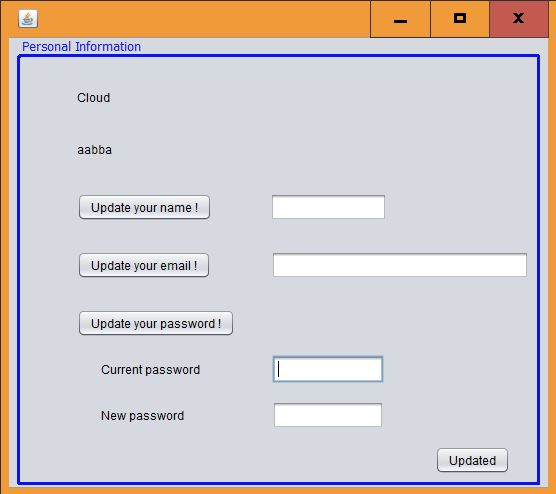
\includegraphics[height=2.5in]{/home/basedul/Documents/Report-writing-using-latex/ResturentManagementSystemReport/modifyc.JPG}
		\caption{Modify admin information window}
		\label{fig:madmin} 
		
		
		\vspace{2cm}
		
		
		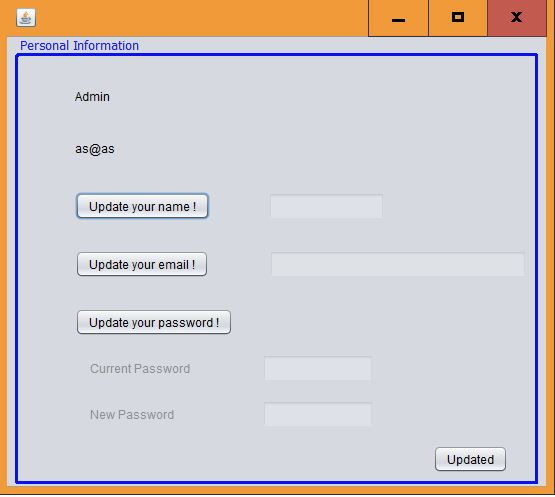
\includegraphics[height=2.5in]{/home/basedul/Documents/Report-writing-using-latex/ResturentManagementSystemReport/modifya.JPG}
		\caption{Modify client information window}
		\label{fig:mclient} 
		\end{figure}	
						
		

	\begin{comment}
	\subsection{Implementing Extreme Programming (XP)}
	As discussed in section \ref{dev:agile}, this project used an agile methodology called Extreme Programming (XP).
This type of methodology utilises an iterative process involving customer communication and feedback.
The iterations were short with a new software version built at the end of each phase. Version control
helped with debugging as the versions could be rolled back to find the iteration that caused the bug.
\subsection{Data Storage and Retrieval}
	As discussed in Section \ref{Rel:RDBMS}, a RDBMS was the preferred storage method chosen for this project. The two
ER diagrams (Figure \ref{fig:entityone} and \ref{fig:entitytwo}) that were designed in Section \ref{sec:entity} helped with the implementation
of the database.\\

The structure of the database was just the first step of many with data retrieval being high in
priority. Recall from the background on requirement gathering (Section \ref{sec:gather}), most software systems
abide by Boehm’s cost model (Figure \ref{fig:req}) so a £1 cost of change in the requirement gathering can cost
up to £1000 in the deployment stage to fix. Therefore when implementing the code to retrieve data
from the database, we have to consider the case that in the future this system will need maintenance
and added features to keep the product competitive within the market. The problem is we cannot
predict the future; all we can do is rely on a well structured code base written using all the skills and
techniques from the field to ensure easy readability of the code.
\\To implement this requirement for database retrieval, the code used the object oriented advantages
of Java to create a database object that provided the database connection and data retrievals. Along
with this database object, inheritance played an important role as a generic class created the SQL
statements using an array of table field names and input values. Any object that required to send or retrieve data to the database could extend this generic class giving that object the functionality to
insert, delete and update any table within the database.

\subsection{GUI Implementation}
The GUI implementation follows on from the GUI designs that were discussed in Section \ref{sec:guiinterface}. Recall,
that the GUI is one of the most important components of the system as it’s the only component the
user will ever interact with. Hence by creating an application that has amazing functionality but in a
poor command line interface would be enough for the user to dislike the software.
The three GUIs have been coded in Java using the Swing classes that are part of the Javax package.
These classes allow applications to be built using similar controls to that found in many applications
therefore first impressions should be recognition of the familiarity of the controls.
The following sub-sections show how some important design concepts were implemented in the
GUI. Code snippets and screenshots will all be used to give a clear explanation of the
implementation.


	\subsubsection{Home Screen}
		\begin{figure}[H]
		\centering
		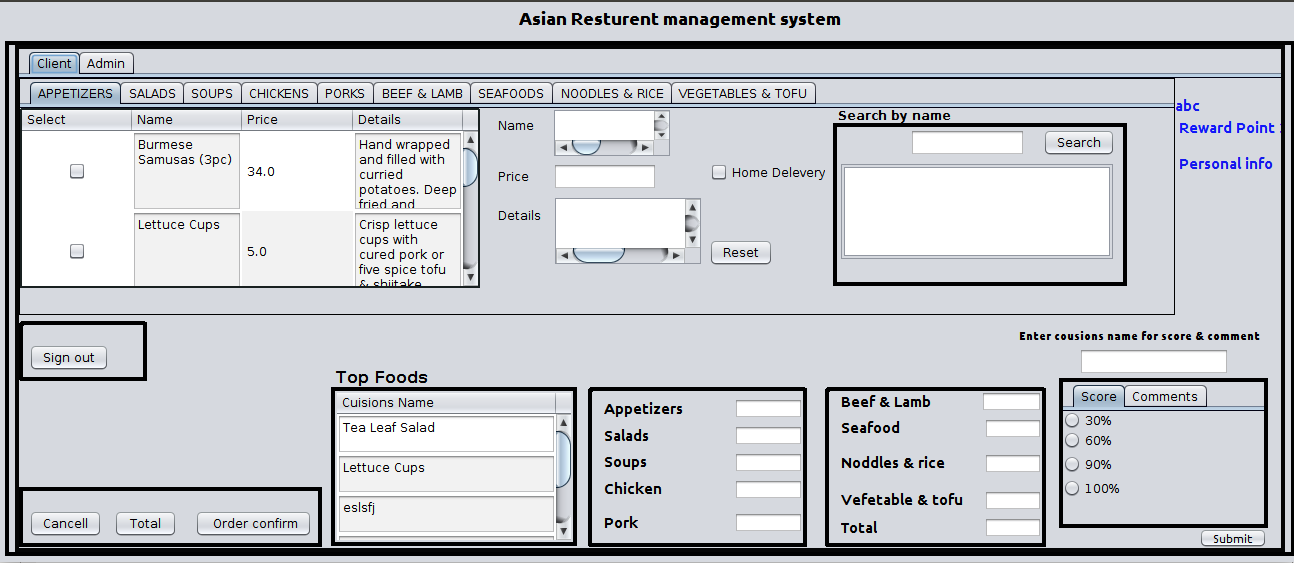
\includegraphics[height=3in]{/home/basedul/Documents/Report-writing-using-latex/ResturentManagementSystemReport/clientGui.png}
		\caption{Design for Home screen}
		\label{fig:homescreen} 
\end{figure}
	\begin{lstlisting}
		/*
 * To change this license header, choose License Headers in Project Properties.
 * To change this template file, choose Tools | Templates
 * and open the template in the editor.
 */
package HomeActivity;

import DatabaseConnection.DatabaseConnection;
import FoodAddOnDatabase.Salads;
import FoodAddOnDatabase.Appetizers;
import FoodAddOnDatabase.BeefLamb;
import FoodAddOnDatabase.Chicken;
import FoodAddOnDatabase.NoddlesRice;
import FoodAddOnDatabase.Pork;
import FoodAddOnDatabase.SeaFood;
import FoodAddOnDatabase.Soups;
import FoodAddOnDatabase.VegeTofu;
import OrderInsertIntoOrderListTable.InsertIntoTable;
import PersonalInfoShow.PersonalInfoFrame;
import PersonalInfoShow.PersonalInfoFrameForAdmin;
import ReadDataFromDatabase.ReadFromTable;
import ReadDataFromDatabase.WrapTextInJTable;
import RegistrationPackage.Admin.SignInClassForAdmin;
import RegistrationPackage.Admin.SignOutForAdmin;
import RegistrationPackage.Admin.SignUpClassForAdmin;
import RegistrationPackage.SignInClass;
import RegistrationPackage.SignOutForClient;
import RegistrationPackage.SignUpClass;
import SearchFromDatabase.SearchFoodInClientModeVege;
import SearchFromDatabase.SearchFromAllDatabase;
import SearchFromDatabase.SearhingInformation;
import java.awt.Dimension;
import java.awt.GraphicsDevice;
import java.awt.GraphicsEnvironment;
import java.awt.Toolkit;
import java.awt.event.ActionEvent;
import java.awt.event.ActionListener;
import java.sql.PreparedStatement;
import java.sql.ResultSet;
import java.sql.SQLException;
import java.util.ArrayList;
import java.util.Random;
import java.util.logging.Level;
import java.util.logging.Logger;
import javax.swing.ButtonGroup;
import javax.swing.JButton;
import javax.swing.JFrame;
import javax.swing.JOptionPane;
import javax.swing.JScrollPane;
import javax.swing.JTable;
import javax.swing.event.TableModelEvent;
import javax.swing.event.TableModelListener;
import javax.swing.table.DefaultTableModel;
import javax.swing.table.TableModel;

/**
 *
 * @author basedul
 */
public class MainActivity extends javax.swing.JFrame implements ActionListener {

    /**
     * Creates new form MainActivity
     *
     */
    String u_score;

    /*Set data on admin table*/
    private StringBuilder meName = new StringBuilder();
    private float totPrice = 0;
    private JScrollPane jScrollPane1;
    private String currentUser = "";
    private String currentAdmin = "";

    StringBuilder str = new StringBuilder();
    StringBuilder str1 = new StringBuilder();
    StringBuilder str2 = new StringBuilder();
    StringBuilder str3 = new StringBuilder();
    StringBuilder str4 = new StringBuilder();
    StringBuilder str5 = new StringBuilder();
    StringBuilder str6 = new StringBuilder();
    StringBuilder str7 = new StringBuilder();
    StringBuilder str8 = new StringBuilder();

    public String getCurrentUser() {
        return currentUser;
    }

    public MainActivity() {
        initComponents();
//        Dimension screenSize = Toolkit.getDefaultToolkit().getScreenSize();
//        setBounds(0,0,screenSize.width, screenSize.height);
//        GraphicsDevice gd = GraphicsEnvironment.getLocalGraphicsEnvironment().getDefaultScreenDevice();
//        int width = gd.getDisplayMode().getWidth();
//        int height = gd.getDisplayMode().getHeight();
//        setBounds(100, 100, width, height);
        setVisible(true);
        setResizable(false);
        setLocationRelativeTo(null);// size of display

        // radio button
        ThirtyP.addActionListener(this);
        SixTyP.addActionListener(this);
        NineTyP.addActionListener(this);
        HundredP.addActionListener(this);
        RadioButtonGroup();

        // table orderList
        /*orderList = new DefaultTableModel();
        orderList.setColumnCount(4);
        orderList.setColumnIdentifiers(new Object[]{"Meal Name", "Drink Name", "Client Name", "Total price"});
        TableForShowOrderList.setModel(orderList);

        // for meal show on cilent side using table
        String qureyM = "select * from `Meal`";
        DefaultTableModel mealListTableModel = new DefaultTableModel();
        mealListTableModel.setColumnIdentifiers(new Object[]{"Name", "Price"});
        new ReadFromTable().ReadMeal(TableForMealInClinet, mealListTableModel, qureyM, "m_name", "m_price");

        // for drink show on cilent side using table
        String qureyD = "select * from `Drink`";
        DefaultTableModel drinkListTableModel = new DefaultTableModel();
        drinkListTableModel.setColumnIdentifiers(new Object[]{"Name", "Price"});
        new ReadFromTable().ReadMeal(TableForSetDrink, drinkListTableModel, qureyD, "d_name", "d_price");
        
        
        
        // for drink show on cilent side using table
        String qureyO = "select * from `OrderList`";
        DefaultTableModel OrderListTableModel = new DefaultTableModel();
        OrderListTableModel.setColumnIdentifiers(new Object[]{"Lunch Specials", "Drinks", "Client Name", "Total price"});
        new ReadFromTable().ReadMeal(TableForShowOrderList, OrderListTableModel, qureyO, "o_m_name", "o_d_name", "o_c_name", "o_t_price");
        // button setClickable or not
        confirmOrderButton.setVisible(false);
        //TableForShowOrderList.setVisible(false);
        
        //ScrollPaneForOrdLisTable.setVisible(false);
        TableForShowOrderList.setVisible(false);*/
        //vage_table();
        String qureyAp = "select * from `APPETIZERS`";
        new ReadFromTable().readFoodsFromTable(apptizers_table, qureyAp, "app_name", "app_price", "details_of_App");

        String qureysl = "select * from `Salad`";
        new ReadFromTable().readFoodsFromTable(saladTable, qureysl, "sl_name", "sl_price", "sl_details");

        String qureysp = "select * from `Soups`";
        new ReadFromTable().readFoodsFromTable(SoupsTable, qureysp, "so_name", "so_price", "so_details");

        String qureyck = "select * from `Chicken`";
        new ReadFromTable().readFoodsFromTable(ChickenTable, qureyck, "ck_name", "ck_price", "ck_details");

        String qureypk = "select * from `Pork`";
        new ReadFromTable().readFoodsFromTable(PorkTable, qureypk, "po_name", "po_price", "po_details");

        String qureybl = "select * from `BeefLamb`";
        new ReadFromTable().readFoodsFromTable(Beef_lambTable, qureybl, "bl_name", "bl_price", "bl_details");

        String qureysf = "select * from `SeaFood`";
        new ReadFromTable().readFoodsFromTable(SeaFoodTable, qureysf, "sf_name", "sf_price", "sf_details");

        String qureynr = "select * from `NoddlesRice`";
        new ReadFromTable().readFoodsFromTable(NoddlesTable, qureynr, "nr_name", "nr_price", "nr_details");

        String qureyvt = "select * from `VegeTofu`";
        new ReadFromTable().readFoodsFromTable(VegeTables, qureyvt, "vt_name", "vt_price", "vt_details");

        confirmOrderButton.setVisible(false);
        //TableForShowOrderList.setVisible(false);

        String qureyO = "select * from `ClientOrderList`";
        DefaultTableModel OrderListTableModel = new DefaultTableModel();
        OrderListTableModel.setColumnIdentifiers(new Object[]{"Cuisions Name", "Price", "Client Name"});
        new ReadFromTable().ReadMeal(TableForShowOrderList, OrderListTableModel, qureyO, "col_name", "col_price", "UserName", 150);

        /**
         * **
         */
        String qureyrl = "select DISTINCT rl_name from `RankList` ORDER BY `rl_score` DESC";
        DefaultTableModel rl = new DefaultTableModel();
        rl.setColumnIdentifiers(new Object[]{"Cuisions Name"});
        new ReadFromTable().ReadMeal(topFoodsTable, rl, qureyrl, "rl_name", 0, 0);

        topFoodsTable.getColumnModel().getColumn(0).setCellRenderer(new WrapTextInJTable());
        int rowRl = topFoodsTable.getRowCount();
        for (int i = 0; i < rowRl; i++) {
            topFoodsTable.setRowHeight(i, 40);
        }
        topFoodsTable.setCellSelectionEnabled(false);

        apptizers_table.getColumnModel().getColumn(1).setCellRenderer(new WrapTextInJTable());
        apptizers_table.getColumnModel().getColumn(3).setCellRenderer(new WrapTextInJTable());
        int rowC = apptizers_table.getRowCount();
        for (int i = 0; i < rowC; i++) {
            apptizers_table.setRowHeight(i, 80);
        }
        apptizers_table.setCellSelectionEnabled(false);

        saladTable.getColumnModel().getColumn(1).setCellRenderer(new WrapTextInJTable());
        saladTable.getColumnModel().getColumn(3).setCellRenderer(new WrapTextInJTable());
        int rowCS = saladTable.getRowCount();
        for (int i = 0; i < rowCS; i++) {
            saladTable.setRowHeight(i, 80);
        }
        saladTable.setCellSelectionEnabled(false);

        SoupsTable.getColumnModel().getColumn(1).setCellRenderer(new WrapTextInJTable());
        SoupsTable.getColumnModel().getColumn(3).setCellRenderer(new WrapTextInJTable());
        int rowCSO = SoupsTable.getRowCount();
        for (int i = 0; i < rowCSO; i++) {
            SoupsTable.setRowHeight(i, 80);
        }
        SoupsTable.setCellSelectionEnabled(false);

        ChickenTable.getColumnModel().getColumn(1).setCellRenderer(new WrapTextInJTable());
        ChickenTable.getColumnModel().getColumn(3).setCellRenderer(new WrapTextInJTable());
        int rowcH = ChickenTable.getRowCount();
        for (int i = 0; i < rowcH; i++) {
            ChickenTable.setRowHeight(i, 80);
        }
        ChickenTable.setCellSelectionEnabled(false);

        Beef_lambTable.getColumnModel().getColumn(1).setCellRenderer(new WrapTextInJTable());
        Beef_lambTable.getColumnModel().getColumn(3).setCellRenderer(new WrapTextInJTable());
        int rowB = Beef_lambTable.getRowCount();
        for (int i = 0; i < rowB; i++) {
            Beef_lambTable.setRowHeight(i, 80);
        }
        Beef_lambTable.setCellSelectionEnabled(false);

        PorkTable.getColumnModel().getColumn(1).setCellRenderer(new WrapTextInJTable());
        PorkTable.getColumnModel().getColumn(3).setCellRenderer(new WrapTextInJTable());
        int rowP = PorkTable.getRowCount();
        for (int i = 0; i < rowP; i++) {
            PorkTable.setRowHeight(i, 80);
        }
        PorkTable.setCellSelectionEnabled(false);

        SeaFoodTable.getColumnModel().getColumn(1).setCellRenderer(new WrapTextInJTable());
        SeaFoodTable.getColumnModel().getColumn(3).setCellRenderer(new WrapTextInJTable());
        int rowSf = SeaFoodTable.getRowCount();
        for (int i = 0; i < rowSf; i++) {
            SeaFoodTable.setRowHeight(i, 80);
        }
        SeaFoodTable.setCellSelectionEnabled(false);

        NoddlesTable.getColumnModel().getColumn(1).setCellRenderer(new WrapTextInJTable());
        NoddlesTable.getColumnModel().getColumn(3).setCellRenderer(new WrapTextInJTable());
        int rownd = NoddlesTable.getRowCount();
        for (int i = 0; i < rownd; i++) {
            NoddlesTable.setRowHeight(i, 80);
        }
        NoddlesTable.setCellSelectionEnabled(false);

        VegeTables.getColumnModel().getColumn(1).setCellRenderer(new WrapTextInJTable());
        VegeTables.getColumnModel().getColumn(3).setCellRenderer(new WrapTextInJTable());
        int rowVG = VegeTables.getRowCount();
        for (int i = 0; i < rowVG; i++) {
            VegeTables.setRowHeight(i, 80);
        }
        VegeTables.setCellSelectionEnabled(false);

        TableForShowOrderList.getColumnModel().getColumn(0).setCellRenderer(new WrapTextInJTable());
        //TableForShowOrderList.getColumnModel().getColumn().setCellRenderer(new WrapTextInJTable());
        int rowAd = TableForShowOrderList.getRowCount();
        for (int i = 0; i < rowAd; i++) {
            TableForShowOrderList.setRowHeight(i, 80);
        }
        TableForShowOrderList.setCellSelectionEnabled(false);

        setActiveUser();
        setActiveAdmin();

    }

    public JButton getConfirmButton() {
        return confirmOrderButton;
    }

    public JTable tableVisibilty() {
        return TableForShowOrderList;
    }

    public void topFoods() {
        String foodName = editTextForCousionsNameSC.getText().toString();
        if (!foodName.equals("")) {
            if (!u_score.equals("")) {
                int score = Integer.parseInt(u_score);
                String comments = editTextComments.getText().toString();
                if (!comments.equals("")) {
                    PreparedStatement ps;
                    String query = "INSERT INTO `RankList`(`rl_name`, `rl_score`, `rl_comments`) VALUES (?,?,?)";
                    try {
                        ps = DatabaseConnection.getConnection().prepareStatement(query);
                        ps.setString(1, foodName);
                        ps.setInt(2, score);
                        ps.setString(3, comments);

                        if (ps.executeUpdate() > 0) {
                            JOptionPane.showMessageDialog(rootPane, "Thank you!");
                        }
                    } catch (SQLException ex) {
                        Logger.getLogger(MainActivity.class.getName()).log(Level.SEVERE, null, ex);
                    }
                } else {
                    JOptionPane.showMessageDialog(rootPane, "Please, enter your comments !");
                    editTextComments.setText("");
                    editTextComments.requestFocus();
                }
            } else {
                JOptionPane.showMessageDialog(rootPane, "Select score !");
                /// selection clear korte hobe
            }
        } else {
            JOptionPane.showMessageDialog(rootPane, "Please enter food name !");
            editTextForCousionsNameSC.setText("");
            editTextForCousionsNameSC.requestFocus();
        }
    }

    public void setActiveAdmin() {
        PreparedStatement ps;
        ResultSet rs;
        String query = "SELECT * FROM `RegistrationForAdmin` WHERE `status` =?";
        try {
            ps = DatabaseConnection.getConnection().prepareStatement(query);
            ps.setInt(1, 1);
            rs = ps.executeQuery();
            if (rs.next()) {
                String name = rs.getString("u_u_name");
                currentAdmin = name;
                activeAdminJlabel.setText(name);
                personalInfoForAdmin.setVisible(true);
                SignInButtonForAdmin.setVisible(false);
                SignUpButtonForAdmin.setVisible(false);
                SignOutButtonForAdmin.setVisible(true);
                ScrollPaneForOrdLisTable.setVisible(true);
            } else {
                activeAdminJlabel.setText("No Admin!");
                personalInfoForAdmin.setVisible(false);
                SignInButtonForAdmin.setVisible(true);
                SignUpButtonForAdmin.setVisible(true);
                ScrollPaneForOrdLisTable.setVisible(false);
                SignOutButtonForAdmin.setVisible(false);
            }
        } catch (SQLException ex) {
            Logger.getLogger(MainActivity.class.getName()).log(Level.SEVERE, null, ex);
        }
    }

    public void setActiveUser() {
        PreparedStatement ps;
        ResultSet rs;
        String query = "SELECT * FROM `Registration` WHERE `status` =?";
        try {
            ps = DatabaseConnection.getConnection().prepareStatement(query);
            ps.setInt(1, 1);
            rs = ps.executeQuery();
            if (rs.next()) {
                String name = rs.getString("u_u_name");
                currentUser = name;
                float rePoint = rs.getFloat("reward_point");
                activeUserJlabel.setText(name);
                rewardPointLabel.setText("Reward Point " + (int) rePoint);
                rewardPointLabel.setVisible(true);
                personalInfo.setVisible(true);
                SignInButton.setVisible(false);
                SignUpButton.setVisible(false);
                SignOutButtonForClient.setVisible(true);
                confirmOrderButton.setVisible(true);
            } else {
                activeUserJlabel.setText("No user!");
                personalInfo.setVisible(false);
                rewardPointLabel.setVisible(false);
                SignInButton.setVisible(true);
                SignUpButton.setVisible(true);
                SignOutButtonForClient.setVisible(false);
            }
        } catch (SQLException ex) {
            Logger.getLogger(MainActivity.class.getName()).log(Level.SEVERE, null, ex);
        }

    }

    public void RadioButtonGroup() {
        ButtonGroup buttonGroup = new ButtonGroup();
        buttonGroup.add(ThirtyP);
        buttonGroup.add(SixTyP);
        buttonGroup.add(NineTyP);
        buttonGroup.add(HundredP);
    }

    /**
     * This method is called from within the constructor to initialize the form.
     * WARNING: Do NOT modify this code. The content of this method is always
     * regenerated by the Form Editor.
     */
    @SuppressWarnings("unchecked")
    // <editor-fold defaultstate="collapsed" desc="Generated Code">                          
    private void initComponents() {

        jPanel8 = new javax.swing.JPanel();
        Admin = new javax.swing.JTabbedPane();
        jPanel1 = new javax.swing.JPanel();
        jPanel7 = new javax.swing.JPanel();
        jLabel7 = new javax.swing.JLabel();
        jLabel8 = new javax.swing.JLabel();
        jLabel4 = new javax.swing.JLabel();
        jLabel5 = new javax.swing.JLabel();
        jLabel6 = new javax.swing.JLabel();
        appTot = new javax.swing.JTextField();
        TotaSalad = new javax.swing.JTextField();
        totaChicken = new javax.swing.JTextField();
        TotaSup = new javax.swing.JTextField();
        totaPork = new javax.swing.JTextField();
        jPanel10 = new javax.swing.JPanel();
        SignInButton = new javax.swing.JButton();
        SignUpButton = new javax.swing.JButton();
        SignOutButtonForClient = new javax.swing.JButton();
        jPanel12 = new javax.swing.JPanel();
        confirmOrderButton = new javax.swing.JButton();
        CancellButton = new javax.swing.JButton();
        TotalButton = new javax.swing.JButton();
        jTabbedPane1 = new javax.swing.JTabbedPane();
        jPanel17 = new javax.swing.JPanel();
        jScrollPane8 = new javax.swing.JScrollPane();
        apptizers_table = new javax.swing.JTable();
        jLabelAp2 = new javax.swing.JLabel();
        jLabel14 = new javax.swing.JLabel();
        jLabel15 = new javax.swing.JLabel();
        priceShowText = new javax.swing.JTextField();
        res_button_app = new javax.swing.JButton();
        homeDel = new javax.swing.JCheckBox();
        jScrollPane6 = new javax.swing.JScrollPane();
        detailsShowTxt = new javax.swing.JTextArea();
        jScrollPane9 = new javax.swing.JScrollPane();
        NameShowText = new javax.swing.JTextArea();
        jPanel15 = new javax.swing.JPanel();
        appGetText = new javax.swing.JTextField();
        SearchButtonInClientForApp = new javax.swing.JButton();
        jScrollPane7 = new javax.swing.JScrollPane();
        jScrollPane34 = new javax.swing.JScrollPane();
        appGetTextForShow = new javax.swing.JTextArea();
        jPanel18 = new javax.swing.JPanel();
        jScrollPane10 = new javax.swing.JScrollPane();
        saladTable = new javax.swing.JTable();
        jLabelAp3 = new javax.swing.JLabel();
        jLabel16 = new javax.swing.JLabel();
        jLabel17 = new javax.swing.JLabel();
        priceShowTextSalad = new javax.swing.JTextField();
        res_button_salad = new javax.swing.JButton();
        home_delv_salad = new javax.swing.JCheckBox();
        jScrollPane11 = new javax.swing.JScrollPane();
        detailsShowTxtSalad = new javax.swing.JTextArea();
        jScrollPane12 = new javax.swing.JScrollPane();
        NameShowTextSalad = new javax.swing.JTextArea();
        jPanel26 = new javax.swing.JPanel();
        saladtextget = new javax.swing.JTextField();
        SearchButtonInClientSalad = new javax.swing.JButton();
        jScrollPane35 = new javax.swing.JScrollPane();
        jScrollPane36 = new javax.swing.JScrollPane();
        saladgetTextShow = new javax.swing.JTextArea();
        jPanel19 = new javax.swing.JPanel();
        jScrollPane13 = new javax.swing.JScrollPane();
        SoupsTable = new javax.swing.JTable();
        jLabelAp4 = new javax.swing.JLabel();
        jLabel18 = new javax.swing.JLabel();
        jLabel19 = new javax.swing.JLabel();
        priceShowTextSoups = new javax.swing.JTextField();
        res_button_soup = new javax.swing.JButton();
        home_delv_soup = new javax.swing.JCheckBox();
        jScrollPane14 = new javax.swing.JScrollPane();
        detailsShowTxtSoups = new javax.swing.JTextArea();
        jScrollPane15 = new javax.swing.JScrollPane();
        NameShowTextSoups = new javax.swing.JTextArea();
        jPanel27 = new javax.swing.JPanel();
        SoupsGetText = new javax.swing.JTextField();
        SoupsSearchButton = new javax.swing.JButton();
        jScrollPane37 = new javax.swing.JScrollPane();
        jScrollPane38 = new javax.swing.JScrollPane();
        SoupsGetTextShow = new javax.swing.JTextArea();
        jPanel20 = new javax.swing.JPanel();
        jScrollPane16 = new javax.swing.JScrollPane();
        ChickenTable = new javax.swing.JTable();
        jLabelAp5 = new javax.swing.JLabel();
        jLabel20 = new javax.swing.JLabel();
        jLabel21 = new javax.swing.JLabel();
        priceShowTextChicken = new javax.swing.JTextField();
        res_button_chick = new javax.swing.JButton();
        home_del_chik = new javax.swing.JCheckBox();
        jScrollPane17 = new javax.swing.JScrollPane();
        detailsShowTxtChicken = new javax.swing.JTextArea();
        jScrollPane18 = new javax.swing.JScrollPane();
        NameShowTextChicken = new javax.swing.JTextArea();
        jPanel28 = new javax.swing.JPanel();
        checkenGetText = new javax.swing.JTextField();
        ChickensearchButton = new javax.swing.JButton();
        jScrollPane39 = new javax.swing.JScrollPane();
        jScrollPane40 = new javax.swing.JScrollPane();
        chickenTextSh = new javax.swing.JTextArea();
        jPanel21 = new javax.swing.JPanel();
        jScrollPane19 = new javax.swing.JScrollPane();
        PorkTable = new javax.swing.JTable();
        jLabelAp6 = new javax.swing.JLabel();
        jLabel22 = new javax.swing.JLabel();
        jLabel23 = new javax.swing.JLabel();
        priceShowTextPork = new javax.swing.JTextField();
        res_butt_pork = new javax.swing.JButton();
        home_delv_pork = new javax.swing.JCheckBox();
        jScrollPane20 = new javax.swing.JScrollPane();
        detailsShowTxtPork = new javax.swing.JTextArea();
        jScrollPane21 = new javax.swing.JScrollPane();
        NameShowTextPork = new javax.swing.JTextArea();
        jPanel29 = new javax.swing.JPanel();
        porkGetT = new javax.swing.JTextField();
        porkSearchButton = new javax.swing.JButton();
        jScrollPane41 = new javax.swing.JScrollPane();
        jScrollPane42 = new javax.swing.JScrollPane();
        porkGetTSh = new javax.swing.JTextArea();
        jPanel22 = new javax.swing.JPanel();
        jScrollPane22 = new javax.swing.JScrollPane();
        Beef_lambTable = new javax.swing.JTable();
        jLabelAp7 = new javax.swing.JLabel();
        jLabel24 = new javax.swing.JLabel();
        jLabel25 = new javax.swing.JLabel();
        priceShowTextBeefLamb = new javax.swing.JTextField();
        res_button_beef = new javax.swing.JButton();
        home_delv_beef = new javax.swing.JCheckBox();
        jScrollPane23 = new javax.swing.JScrollPane();
        detailsShowTxtBeefLamb = new javax.swing.JTextArea();
        jScrollPane24 = new javax.swing.JScrollPane();
        NameShowTextBeefLamb = new javax.swing.JTextArea();
        jPanel30 = new javax.swing.JPanel();
        beefText = new javax.swing.JTextField();
        beefSearchButton = new javax.swing.JButton();
        jScrollPane43 = new javax.swing.JScrollPane();
        jScrollPane44 = new javax.swing.JScrollPane();
        beefTextShw = new javax.swing.JTextArea();
        jPanel23 = new javax.swing.JPanel();
        jScrollPane25 = new javax.swing.JScrollPane();
        SeaFoodTable = new javax.swing.JTable();
        jLabelAp8 = new javax.swing.JLabel();
        jLabel26 = new javax.swing.JLabel();
        jLabel27 = new javax.swing.JLabel();
        priceShowTextSeaFood = new javax.swing.JTextField();
        res_button_sea = new javax.swing.JButton();
        home_delv_sea = new javax.swing.JCheckBox();
        jScrollPane26 = new javax.swing.JScrollPane();
        detailsShowTxtSeaFood = new javax.swing.JTextArea();
        jScrollPane27 = new javax.swing.JScrollPane();
        NameShowTextSeaFood = new javax.swing.JTextArea();
        jPanel31 = new javax.swing.JPanel();
        seaText = new javax.swing.JTextField();
        seaSearchButton = new javax.swing.JButton();
        jScrollPane45 = new javax.swing.JScrollPane();
        jScrollPane46 = new javax.swing.JScrollPane();
        seaTextShow = new javax.swing.JTextArea();
        jPanel24 = new javax.swing.JPanel();
        jScrollPane28 = new javax.swing.JScrollPane();
        NoddlesTable = new javax.swing.JTable();
        jLabelAp9 = new javax.swing.JLabel();
        jLabel28 = new javax.swing.JLabel();
        jLabel29 = new javax.swing.JLabel();
        priceShowTextNoddlesRice = new javax.swing.JTextField();
        res_button_nodd = new javax.swing.JButton();
        home_delv_nodd = new javax.swing.JCheckBox();
        jScrollPane29 = new javax.swing.JScrollPane();
        detailsShowTxtNoddlesRice = new javax.swing.JTextArea();
        jScrollPane30 = new javax.swing.JScrollPane();
        NameShowTextNoddlesRice = new javax.swing.JTextArea();
        jPanel32 = new javax.swing.JPanel();
        nodText = new javax.swing.JTextField();
        nodSearchButton = new javax.swing.JButton();
        jScrollPane47 = new javax.swing.JScrollPane();
        jScrollPane48 = new javax.swing.JScrollPane();
        nodTextShow = new javax.swing.JTextArea();
        jPanel25 = new javax.swing.JPanel();
        jScrollPane31 = new javax.swing.JScrollPane();
        VegeTables = new javax.swing.JTable();
        jLabelAp10 = new javax.swing.JLabel();
        jLabel30 = new javax.swing.JLabel();
        jLabel31 = new javax.swing.JLabel();
        priceShowTextvege = new javax.swing.JTextField();
        res_button_vege = new javax.swing.JButton();
        home_delv_vege = new javax.swing.JCheckBox();
        jScrollPane32 = new javax.swing.JScrollPane();
        detailsShowTxtvege = new javax.swing.JTextArea();
        jScrollPane33 = new javax.swing.JScrollPane();
        NameShowTextvege = new javax.swing.JTextArea();
        jPanel11 = new javax.swing.JPanel();
        vegeGetText = new javax.swing.JTextField();
        SearchButtonInClientForVEGe = new javax.swing.JButton();
        jScrollPane3 = new javax.swing.JScrollPane();
        jScrollPane4 = new javax.swing.JScrollPane();
        vegeGetTextForShow = new javax.swing.JTextArea();
        jPanel9 = new javax.swing.JPanel();
        jLabel9 = new javax.swing.JLabel();
        jLabel11 = new javax.swing.JLabel();
        jLabel12 = new javax.swing.JLabel();
        jLabel13 = new javax.swing.JLabel();
        jLabel32 = new javax.swing.JLabel();
        totaBeef = new javax.swing.JTextField();
        totaSea = new javax.swing.JTextField();
        totaVege = new javax.swing.JTextField();
        totaNodd = new javax.swing.JTextField();
        tota = new javax.swing.JTextField();
        activeUserJlabel = new javax.swing.JLabel();
        jTabbedPane2 = new javax.swing.JTabbedPane();
        jPanel5 = new javax.swing.JPanel();
        ThirtyP = new javax.swing.JRadioButton();
        SixTyP = new javax.swing.JRadioButton();
        NineTyP = new javax.swing.JRadioButton();
        HundredP = new javax.swing.JRadioButton();
        jPanel6 = new javax.swing.JPanel();
        editTextComments = new javax.swing.JTextField();
        jLabel2 = new javax.swing.JLabel();
        personalInfo = new javax.swing.JLabel();
        jLabel1 = new javax.swing.JLabel();
        editTextForCousionsNameSC = new javax.swing.JTextField();
        buttonSubmitSC = new javax.swing.JButton();
        ScrollPaneForOrdLisTable1 = new javax.swing.JScrollPane();
        topFoodsTable = new javax.swing.JTable();
        rewardPointLabel = new javax.swing.JLabel();
        jPanel4 = new javax.swing.JPanel();
        jPanel13 = new javax.swing.JPanel();
        SignInButtonForAdmin = new javax.swing.JButton();
        SignUpButtonForAdmin = new javax.swing.JButton();
        SignOutButtonForAdmin = new javax.swing.JButton();
        ScrollPaneForOrdLisTable = new javax.swing.JScrollPane();
        TableForShowOrderList = new javax.swing.JTable();
        jPanel16 = new javax.swing.JPanel();
        addAppetizersButton = new javax.swing.JButton();
        addDrinksButton = new javax.swing.JButton();
        SoupsAddButton = new javax.swing.JButton();
        ChickenAddButton = new javax.swing.JButton();
        PorkAddButton = new javax.swing.JButton();
        Beef_LambAddButton = new javax.swing.JButton();
        SeaFoodAddButton = new javax.swing.JButton();
        Noddles_RiceAddButton = new javax.swing.JButton();
        Vegetables_tofuAddButton = new javax.swing.JButton();
        activeAdminJlabel = new javax.swing.JLabel();
        personalInfoForAdmin = new javax.swing.JLabel();
        jLabel3 = new javax.swing.JLabel();

        setDefaultCloseOperation(javax.swing.WindowConstants.EXIT_ON_CLOSE);

        jPanel8.setBorder(javax.swing.BorderFactory.createLineBorder(new java.awt.Color(0, 0, 0), 4));

        Admin.setBorder(javax.swing.BorderFactory.createMatteBorder(4, 4, 4, 4, new java.awt.Color(5, 5, 5)));
        Admin.addMouseListener(new java.awt.event.MouseAdapter() {
            public void mouseClicked(java.awt.event.MouseEvent evt) {
                AdminMouseClicked(evt);
            }
        });

        jPanel1.setLayout(new org.netbeans.lib.awtextra.AbsoluteLayout());

        jPanel7.setBorder(new javax.swing.border.LineBorder(new java.awt.Color(0, 0, 0), 4, true));

        jLabel7.setFont(new java.awt.Font("Ubuntu", 1, 15)); // NOI18N
        jLabel7.setText("Pork");

        jLabel8.setFont(new java.awt.Font("Ubuntu", 1, 15)); // NOI18N
        jLabel8.setText("Chicken");

        jLabel4.setFont(new java.awt.Font("Ubuntu", 1, 15)); // NOI18N
        jLabel4.setText("Appetizers");

        jLabel5.setFont(new java.awt.Font("Ubuntu", 1, 15)); // NOI18N
        jLabel5.setText("Salads");

        jLabel6.setFont(new java.awt.Font("Ubuntu", 1, 15)); // NOI18N
        jLabel6.setText("Soups");

        javax.swing.GroupLayout jPanel7Layout = new javax.swing.GroupLayout(jPanel7);
        jPanel7.setLayout(jPanel7Layout);
        jPanel7Layout.setHorizontalGroup(
            jPanel7Layout.createParallelGroup(javax.swing.GroupLayout.Alignment.LEADING)
            .addGroup(jPanel7Layout.createSequentialGroup()
                .addGap(12, 12, 12)
                .addGroup(jPanel7Layout.createParallelGroup(javax.swing.GroupLayout.Alignment.LEADING)
                    .addGroup(jPanel7Layout.createSequentialGroup()
                        .addComponent(jLabel4)
                        .addGap(51, 51, 51)
                        .addComponent(appTot, javax.swing.GroupLayout.PREFERRED_SIZE, 69, javax.swing.GroupLayout.PREFERRED_SIZE))
                    .addGroup(jPanel7Layout.createSequentialGroup()
                        .addComponent(jLabel5)
                        .addGap(85, 85, 85)
                        .addComponent(TotaSalad, javax.swing.GroupLayout.PREFERRED_SIZE, 69, javax.swing.GroupLayout.PREFERRED_SIZE))
                    .addGroup(jPanel7Layout.createSequentialGroup()
                        .addComponent(jLabel6)
                        .addGap(87, 87, 87)
                        .addComponent(TotaSup, javax.swing.GroupLayout.PREFERRED_SIZE, 69, javax.swing.GroupLayout.PREFERRED_SIZE))
                    .addGroup(jPanel7Layout.createSequentialGroup()
                        .addComponent(jLabel8)
                        .addGap(72, 72, 72)
                        .addComponent(totaChicken, javax.swing.GroupLayout.PREFERRED_SIZE, 69, javax.swing.GroupLayout.PREFERRED_SIZE))
                    .addGroup(jPanel7Layout.createSequentialGroup()
                        .addComponent(jLabel7)
                        .addGap(96, 96, 96)
                        .addComponent(totaPork, javax.swing.GroupLayout.PREFERRED_SIZE, 69, javax.swing.GroupLayout.PREFERRED_SIZE))))
        );
        jPanel7Layout.setVerticalGroup(
            jPanel7Layout.createParallelGroup(javax.swing.GroupLayout.Alignment.LEADING)
            .addGroup(jPanel7Layout.createSequentialGroup()
                .addGap(7, 7, 7)
                .addGroup(jPanel7Layout.createParallelGroup(javax.swing.GroupLayout.Alignment.LEADING)
                    .addGroup(jPanel7Layout.createSequentialGroup()
                        .addGap(1, 1, 1)
                        .addComponent(jLabel4))
                    .addComponent(appTot, javax.swing.GroupLayout.PREFERRED_SIZE, 21, javax.swing.GroupLayout.PREFERRED_SIZE))
                .addGap(6, 6, 6)
                .addGroup(jPanel7Layout.createParallelGroup(javax.swing.GroupLayout.Alignment.LEADING)
                    .addGroup(jPanel7Layout.createSequentialGroup()
                        .addGap(1, 1, 1)
                        .addComponent(jLabel5))
                    .addComponent(TotaSalad, javax.swing.GroupLayout.PREFERRED_SIZE, 21, javax.swing.GroupLayout.PREFERRED_SIZE))
                .addGap(6, 6, 6)
                .addGroup(jPanel7Layout.createParallelGroup(javax.swing.GroupLayout.Alignment.LEADING)
                    .addComponent(jLabel6)
                    .addComponent(TotaSup, javax.swing.GroupLayout.PREFERRED_SIZE, 21, javax.swing.GroupLayout.PREFERRED_SIZE))
                .addGap(6, 6, 6)
                .addGroup(jPanel7Layout.createParallelGroup(javax.swing.GroupLayout.Alignment.LEADING)
                    .addComponent(jLabel8)
                    .addComponent(totaChicken, javax.swing.GroupLayout.PREFERRED_SIZE, 21, javax.swing.GroupLayout.PREFERRED_SIZE))
                .addGap(12, 12, 12)
                .addGroup(jPanel7Layout.createParallelGroup(javax.swing.GroupLayout.Alignment.LEADING)
                    .addGroup(jPanel7Layout.createSequentialGroup()
                        .addGap(1, 1, 1)
                        .addComponent(jLabel7))
                    .addComponent(totaPork, javax.swing.GroupLayout.PREFERRED_SIZE, 21, javax.swing.GroupLayout.PREFERRED_SIZE))
                .addContainerGap(javax.swing.GroupLayout.DEFAULT_SIZE, Short.MAX_VALUE))
        );

        jPanel1.add(jPanel7, new org.netbeans.lib.awtextra.AbsoluteConstraints(569, 309, -1, 160));

        jPanel10.setBorder(new javax.swing.border.LineBorder(new java.awt.Color(0, 0, 0), 4, true));

        SignInButton.setText("Sign in");
        SignInButton.addMouseListener(new java.awt.event.MouseAdapter() {
            public void mouseClicked(java.awt.event.MouseEvent evt) {
                SignInButtonMouseClicked(evt);
            }
        });
        SignInButton.addActionListener(new java.awt.event.ActionListener() {
            public void actionPerformed(java.awt.event.ActionEvent evt) {
                SignInButtonActionPerformed(evt);
            }
        });

        SignUpButton.setText("Sign up");
        SignUpButton.addMouseListener(new java.awt.event.MouseAdapter() {
            public void mouseClicked(java.awt.event.MouseEvent evt) {
                SignUpButtonMouseClicked(evt);
            }
        });

        SignOutButtonForClient.setText("Sign out");
        SignOutButtonForClient.addMouseListener(new java.awt.event.MouseAdapter() {
            public void mouseClicked(java.awt.event.MouseEvent evt) {
                SignOutButtonForClientMouseClicked(evt);
            }
        });

        javax.swing.GroupLayout jPanel10Layout = new javax.swing.GroupLayout(jPanel10);
        jPanel10.setLayout(jPanel10Layout);
        jPanel10Layout.setHorizontalGroup(
            jPanel10Layout.createParallelGroup(javax.swing.GroupLayout.Alignment.LEADING)
            .addGroup(javax.swing.GroupLayout.Alignment.TRAILING, jPanel10Layout.createSequentialGroup()
                .addGap(6, 6, 6)
                .addComponent(SignUpButton)
                .addPreferredGap(javax.swing.LayoutStyle.ComponentPlacement.RELATED)
                .addComponent(SignOutButtonForClient)
                .addPreferredGap(javax.swing.LayoutStyle.ComponentPlacement.RELATED, 12, Short.MAX_VALUE)
                .addComponent(SignInButton)
                .addGap(22, 22, 22))
        );
        jPanel10Layout.setVerticalGroup(
            jPanel10Layout.createParallelGroup(javax.swing.GroupLayout.Alignment.LEADING)
            .addGroup(javax.swing.GroupLayout.Alignment.TRAILING, jPanel10Layout.createSequentialGroup()
                .addContainerGap(javax.swing.GroupLayout.DEFAULT_SIZE, Short.MAX_VALUE)
                .addGroup(jPanel10Layout.createParallelGroup(javax.swing.GroupLayout.Alignment.BASELINE)
                    .addComponent(SignInButton)
                    .addComponent(SignUpButton)
                    .addComponent(SignOutButtonForClient))
                .addContainerGap())
        );

        jPanel1.add(jPanel10, new org.netbeans.lib.awtextra.AbsoluteConstraints(0, 243, -1, 60));

        jPanel12.setBorder(javax.swing.BorderFactory.createLineBorder(new java.awt.Color(0, 0, 0), 4));

        confirmOrderButton.setText(" Order confirm");
        confirmOrderButton.addMouseListener(new java.awt.event.MouseAdapter() {
            public void mouseClicked(java.awt.event.MouseEvent evt) {
                confirmOrderButtonMouseClicked(evt);
            }
        });

        CancellButton.setText("Cancell");
        CancellButton.addMouseListener(new java.awt.event.MouseAdapter() {
            public void mouseClicked(java.awt.event.MouseEvent evt) {
                CancellButtonMouseClicked(evt);
            }
        });

        TotalButton.setText("Total");
        TotalButton.addMouseListener(new java.awt.event.MouseAdapter() {
            public void mouseClicked(java.awt.event.MouseEvent evt) {
                TotalButtonMouseClicked(evt);
            }
        });

        javax.swing.GroupLayout jPanel12Layout = new javax.swing.GroupLayout(jPanel12);
        jPanel12.setLayout(jPanel12Layout);
        jPanel12Layout.setHorizontalGroup(
            jPanel12Layout.createParallelGroup(javax.swing.GroupLayout.Alignment.LEADING)
            .addGroup(javax.swing.GroupLayout.Alignment.TRAILING, jPanel12Layout.createSequentialGroup()
                .addContainerGap()
                .addComponent(CancellButton)
                .addPreferredGap(javax.swing.LayoutStyle.ComponentPlacement.UNRELATED)
                .addComponent(TotalButton, javax.swing.GroupLayout.DEFAULT_SIZE, 63, Short.MAX_VALUE)
                .addGap(18, 18, 18)
                .addComponent(confirmOrderButton)
                .addContainerGap())
        );
        jPanel12Layout.setVerticalGroup(
            jPanel12Layout.createParallelGroup(javax.swing.GroupLayout.Alignment.LEADING)
            .addGroup(jPanel12Layout.createSequentialGroup()
                .addContainerGap(javax.swing.GroupLayout.DEFAULT_SIZE, Short.MAX_VALUE)
                .addGroup(jPanel12Layout.createParallelGroup(javax.swing.GroupLayout.Alignment.BASELINE)
                    .addComponent(confirmOrderButton)
                    .addComponent(TotalButton)
                    .addComponent(CancellButton))
                .addContainerGap())
        );

        jPanel1.add(jPanel12, new org.netbeans.lib.awtextra.AbsoluteConstraints(0, 409, -1, 60));

        jTabbedPane1.setBorder(javax.swing.BorderFactory.createLineBorder(new java.awt.Color(0, 0, 0)));

        jScrollPane8.setBorder(new javax.swing.border.LineBorder(new java.awt.Color(24, 32, 32), 2, true));

        apptizers_table.setModel(new javax.swing.table.DefaultTableModel(
            new Object [][] {
                {null, null, null, null},
                {null, null, null, null},
                {null, null, null, null},
                {null, null, null, null}
            },
            new String [] {
                "Title 1", "Title 2", "Title 3", "Title 4"
            }
        ));
        apptizers_table.addMouseListener(new java.awt.event.MouseAdapter() {
            public void mouseClicked(java.awt.event.MouseEvent evt) {
                apptizers_tableMouseClicked(evt);
            }
        });
        jScrollPane8.setViewportView(apptizers_table);

        jLabelAp2.setText("Details");

        jLabel14.setText("Name");

        jLabel15.setText("Price");

        res_button_app.setText("Reset");
        res_button_app.addMouseListener(new java.awt.event.MouseAdapter() {
            public void mouseClicked(java.awt.event.MouseEvent evt) {
                res_button_appMouseClicked(evt);
            }
        });

        homeDel.setText("Home Delevery");

        detailsShowTxt.setColumns(20);
        detailsShowTxt.setRows(5);
        jScrollPane6.setViewportView(detailsShowTxt);

        NameShowText.setColumns(20);
        NameShowText.setRows(5);
        jScrollPane9.setViewportView(NameShowText);

        jPanel15.setBorder(javax.swing.BorderFactory.createTitledBorder(javax.swing.BorderFactory.createLineBorder(new java.awt.Color(0, 0, 0), 4), "Search by name", javax.swing.border.TitledBorder.DEFAULT_JUSTIFICATION, javax.swing.border.TitledBorder.DEFAULT_POSITION, new java.awt.Font("Dialog", 1, 12))); // NOI18N

        SearchButtonInClientForApp.setText("Search");
        SearchButtonInClientForApp.addMouseListener(new java.awt.event.MouseAdapter() {
            public void mouseClicked(java.awt.event.MouseEvent evt) {
                SearchButtonInClientForAppMouseClicked(evt);
            }
        });
        SearchButtonInClientForApp.addActionListener(new java.awt.event.ActionListener() {
            public void actionPerformed(java.awt.event.ActionEvent evt) {
                SearchButtonInClientForAppActionPerformed(evt);
            }
        });

        appGetTextForShow.setColumns(20);
        appGetTextForShow.setRows(5);
        jScrollPane34.setViewportView(appGetTextForShow);

        jScrollPane7.setViewportView(jScrollPane34);

        javax.swing.GroupLayout jPanel15Layout = new javax.swing.GroupLayout(jPanel15);
        jPanel15.setLayout(jPanel15Layout);
        jPanel15Layout.setHorizontalGroup(
            jPanel15Layout.createParallelGroup(javax.swing.GroupLayout.Alignment.LEADING)
            .addGroup(jPanel15Layout.createSequentialGroup()
                .addGap(71, 71, 71)
                .addComponent(appGetText, javax.swing.GroupLayout.PREFERRED_SIZE, 115, javax.swing.GroupLayout.PREFERRED_SIZE)
                .addGap(18, 18, 18)
                .addComponent(SearchButtonInClientForApp, javax.swing.GroupLayout.PREFERRED_SIZE, 72, javax.swing.GroupLayout.PREFERRED_SIZE)
                .addContainerGap(javax.swing.GroupLayout.DEFAULT_SIZE, Short.MAX_VALUE))
            .addGroup(jPanel15Layout.createSequentialGroup()
                .addComponent(jScrollPane7)
                .addContainerGap())
        );
        jPanel15Layout.setVerticalGroup(
            jPanel15Layout.createParallelGroup(javax.swing.GroupLayout.Alignment.LEADING)
            .addGroup(jPanel15Layout.createSequentialGroup()
                .addGroup(jPanel15Layout.createParallelGroup(javax.swing.GroupLayout.Alignment.BASELINE)
                    .addComponent(appGetText, javax.swing.GroupLayout.PREFERRED_SIZE, javax.swing.GroupLayout.DEFAULT_SIZE, javax.swing.GroupLayout.PREFERRED_SIZE)
                    .addComponent(SearchButtonInClientForApp))
                .addPreferredGap(javax.swing.LayoutStyle.ComponentPlacement.RELATED)
                .addComponent(jScrollPane7, javax.swing.GroupLayout.PREFERRED_SIZE, javax.swing.GroupLayout.DEFAULT_SIZE, javax.swing.GroupLayout.PREFERRED_SIZE)
                .addGap(0, 19, Short.MAX_VALUE))
        );

        javax.swing.GroupLayout jPanel17Layout = new javax.swing.GroupLayout(jPanel17);
        jPanel17.setLayout(jPanel17Layout);
        jPanel17Layout.setHorizontalGroup(
            jPanel17Layout.createParallelGroup(javax.swing.GroupLayout.Alignment.LEADING)
            .addGroup(jPanel17Layout.createSequentialGroup()
                .addComponent(jScrollPane8, javax.swing.GroupLayout.PREFERRED_SIZE, 460, javax.swing.GroupLayout.PREFERRED_SIZE)
                .addGap(18, 18, 18)
                .addGroup(jPanel17Layout.createParallelGroup(javax.swing.GroupLayout.Alignment.LEADING)
                    .addGroup(jPanel17Layout.createSequentialGroup()
                        .addComponent(jLabelAp2, javax.swing.GroupLayout.PREFERRED_SIZE, 49, javax.swing.GroupLayout.PREFERRED_SIZE)
                        .addPreferredGap(javax.swing.LayoutStyle.ComponentPlacement.RELATED)
                        .addComponent(jScrollPane6, javax.swing.GroupLayout.PREFERRED_SIZE, 150, javax.swing.GroupLayout.PREFERRED_SIZE)
                        .addPreferredGap(javax.swing.LayoutStyle.ComponentPlacement.RELATED)
                        .addComponent(res_button_app))
                    .addGroup(jPanel17Layout.createSequentialGroup()
                        .addGroup(jPanel17Layout.createParallelGroup(javax.swing.GroupLayout.Alignment.LEADING)
                            .addGroup(jPanel17Layout.createSequentialGroup()
                                .addComponent(jLabel15, javax.swing.GroupLayout.PREFERRED_SIZE, 49, javax.swing.GroupLayout.PREFERRED_SIZE)
                                .addPreferredGap(javax.swing.LayoutStyle.ComponentPlacement.RELATED)
                                .addComponent(priceShowText, javax.swing.GroupLayout.PREFERRED_SIZE, 104, javax.swing.GroupLayout.PREFERRED_SIZE))
                            .addGroup(jPanel17Layout.createSequentialGroup()
                                .addComponent(jLabel14)
                                .addGap(18, 18, 18)
                                .addComponent(jScrollPane9, javax.swing.GroupLayout.PREFERRED_SIZE, 120, javax.swing.GroupLayout.PREFERRED_SIZE)))
                        .addGap(38, 38, 38)
                        .addComponent(homeDel)))
                .addPreferredGap(javax.swing.LayoutStyle.ComponentPlacement.RELATED)
                .addComponent(jPanel15, javax.swing.GroupLayout.PREFERRED_SIZE, javax.swing.GroupLayout.DEFAULT_SIZE, javax.swing.GroupLayout.PREFERRED_SIZE)
                .addGap(0, 0, Short.MAX_VALUE))
        );
        jPanel17Layout.setVerticalGroup(
            jPanel17Layout.createParallelGroup(javax.swing.GroupLayout.Alignment.LEADING)
            .addGroup(jPanel17Layout.createSequentialGroup()
                .addGroup(jPanel17Layout.createParallelGroup(javax.swing.GroupLayout.Alignment.TRAILING)
                    .addComponent(jPanel15, javax.swing.GroupLayout.PREFERRED_SIZE, javax.swing.GroupLayout.DEFAULT_SIZE, javax.swing.GroupLayout.PREFERRED_SIZE)
                    .addGroup(jPanel17Layout.createParallelGroup(javax.swing.GroupLayout.Alignment.LEADING)
                        .addComponent(jScrollPane8, javax.swing.GroupLayout.PREFERRED_SIZE, 180, javax.swing.GroupLayout.PREFERRED_SIZE)
                        .addGroup(jPanel17Layout.createParallelGroup(javax.swing.GroupLayout.Alignment.TRAILING)
                            .addGroup(jPanel17Layout.createSequentialGroup()
                                .addGap(47, 47, 47)
                                .addComponent(homeDel)
                                .addGap(58, 58, 58)
                                .addComponent(res_button_app))
                            .addGroup(jPanel17Layout.createSequentialGroup()
                                .addGroup(jPanel17Layout.createParallelGroup(javax.swing.GroupLayout.Alignment.LEADING)
                                    .addGroup(jPanel17Layout.createSequentialGroup()
                                        .addGap(10, 10, 10)
                                        .addComponent(jLabel14))
                                    .addComponent(jScrollPane9, javax.swing.GroupLayout.PREFERRED_SIZE, 50, javax.swing.GroupLayout.PREFERRED_SIZE))
                                .addGap(5, 5, 5)
                                .addGroup(jPanel17Layout.createParallelGroup(javax.swing.GroupLayout.Alignment.BASELINE)
                                    .addComponent(jLabel15)
                                    .addComponent(priceShowText, javax.swing.GroupLayout.PREFERRED_SIZE, javax.swing.GroupLayout.DEFAULT_SIZE, javax.swing.GroupLayout.PREFERRED_SIZE))
                                .addGroup(jPanel17Layout.createParallelGroup(javax.swing.GroupLayout.Alignment.LEADING)
                                    .addGroup(jPanel17Layout.createSequentialGroup()
                                        .addGap(18, 18, 18)
                                        .addComponent(jLabelAp2))
                                    .addGroup(jPanel17Layout.createSequentialGroup()
                                        .addPreferredGap(javax.swing.LayoutStyle.ComponentPlacement.RELATED)
                                        .addComponent(jScrollPane6, javax.swing.GroupLayout.PREFERRED_SIZE, 70, javax.swing.GroupLayout.PREFERRED_SIZE)))))))
                .addGap(129, 129, 129))
        );

        jTabbedPane1.addTab("APPETIZERS", jPanel17);

        jScrollPane10.setBorder(new javax.swing.border.LineBorder(new java.awt.Color(20, 224, 240), 2, true));

        saladTable.setModel(new javax.swing.table.DefaultTableModel(
            new Object [][] {
                {null, null, null, null},
                {null, null, null, null},
                {null, null, null, null},
                {null, null, null, null}
            },
            new String [] {
                "Title 1", "Title 2", "Title 3", "Title 4"
            }
        ));
        saladTable.addMouseListener(new java.awt.event.MouseAdapter() {
            public void mouseClicked(java.awt.event.MouseEvent evt) {
                saladTableMouseClicked(evt);
            }
        });
        jScrollPane10.setViewportView(saladTable);
        if (saladTable.getColumnModel().getColumnCount() > 0) {
            saladTable.getColumnModel().getColumn(3).setHeaderValue("Title 4");
        }

        jLabelAp3.setText("Details");

        jLabel16.setText("Name");

        jLabel17.setText("Price");

        res_button_salad.setText("Reset");
        res_button_salad.addMouseListener(new java.awt.event.MouseAdapter() {
            public void mouseClicked(java.awt.event.MouseEvent evt) {
                res_button_saladMouseClicked(evt);
            }
        });

        home_delv_salad.setText("Home Delevery");

        detailsShowTxtSalad.setColumns(20);
        detailsShowTxtSalad.setRows(5);
        jScrollPane11.setViewportView(detailsShowTxtSalad);

        NameShowTextSalad.setColumns(20);
        NameShowTextSalad.setRows(5);
        jScrollPane12.setViewportView(NameShowTextSalad);

        jPanel26.setBorder(javax.swing.BorderFactory.createTitledBorder(javax.swing.BorderFactory.createLineBorder(new java.awt.Color(0, 0, 0), 4), "Search by name", javax.swing.border.TitledBorder.DEFAULT_JUSTIFICATION, javax.swing.border.TitledBorder.DEFAULT_POSITION, new java.awt.Font("Dialog", 1, 12))); // NOI18N

        SearchButtonInClientSalad.setText("Search");
        SearchButtonInClientSalad.addMouseListener(new java.awt.event.MouseAdapter() {
            public void mouseClicked(java.awt.event.MouseEvent evt) {
                SearchButtonInClientSaladMouseClicked(evt);
            }
        });
        SearchButtonInClientSalad.addActionListener(new java.awt.event.ActionListener() {
            public void actionPerformed(java.awt.event.ActionEvent evt) {
                SearchButtonInClientSaladActionPerformed(evt);
            }
        });

        saladgetTextShow.setColumns(20);
        saladgetTextShow.setRows(5);
        jScrollPane36.setViewportView(saladgetTextShow);

        jScrollPane35.setViewportView(jScrollPane36);

        javax.swing.GroupLayout jPanel26Layout = new javax.swing.GroupLayout(jPanel26);
        jPanel26.setLayout(jPanel26Layout);
        jPanel26Layout.setHorizontalGroup(
            jPanel26Layout.createParallelGroup(javax.swing.GroupLayout.Alignment.LEADING)
            .addGroup(jPanel26Layout.createSequentialGroup()
                .addGap(71, 71, 71)
                .addComponent(saladtextget, javax.swing.GroupLayout.PREFERRED_SIZE, 115, javax.swing.GroupLayout.PREFERRED_SIZE)
                .addGap(18, 18, 18)
                .addComponent(SearchButtonInClientSalad, javax.swing.GroupLayout.PREFERRED_SIZE, 72, javax.swing.GroupLayout.PREFERRED_SIZE)
                .addContainerGap(javax.swing.GroupLayout.DEFAULT_SIZE, Short.MAX_VALUE))
            .addGroup(jPanel26Layout.createSequentialGroup()
                .addComponent(jScrollPane35)
                .addContainerGap())
        );
        jPanel26Layout.setVerticalGroup(
            jPanel26Layout.createParallelGroup(javax.swing.GroupLayout.Alignment.LEADING)
            .addGroup(jPanel26Layout.createSequentialGroup()
                .addGroup(jPanel26Layout.createParallelGroup(javax.swing.GroupLayout.Alignment.BASELINE)
                    .addComponent(saladtextget, javax.swing.GroupLayout.PREFERRED_SIZE, javax.swing.GroupLayout.DEFAULT_SIZE, javax.swing.GroupLayout.PREFERRED_SIZE)
                    .addComponent(SearchButtonInClientSalad))
                .addPreferredGap(javax.swing.LayoutStyle.ComponentPlacement.RELATED)
                .addComponent(jScrollPane35, javax.swing.GroupLayout.PREFERRED_SIZE, javax.swing.GroupLayout.DEFAULT_SIZE, javax.swing.GroupLayout.PREFERRED_SIZE)
                .addGap(0, 19, Short.MAX_VALUE))
        );

        javax.swing.GroupLayout jPanel18Layout = new javax.swing.GroupLayout(jPanel18);
        jPanel18.setLayout(jPanel18Layout);
        jPanel18Layout.setHorizontalGroup(
            jPanel18Layout.createParallelGroup(javax.swing.GroupLayout.Alignment.LEADING)
            .addGroup(jPanel18Layout.createSequentialGroup()
                .addComponent(jScrollPane10, javax.swing.GroupLayout.PREFERRED_SIZE, 460, javax.swing.GroupLayout.PREFERRED_SIZE)
                .addGap(18, 18, 18)
                .addGroup(jPanel18Layout.createParallelGroup(javax.swing.GroupLayout.Alignment.LEADING)
                    .addComponent(jLabel16)
                    .addComponent(jLabel17, javax.swing.GroupLayout.PREFERRED_SIZE, 49, javax.swing.GroupLayout.PREFERRED_SIZE)
                    .addComponent(jLabelAp3, javax.swing.GroupLayout.PREFERRED_SIZE, 49, javax.swing.GroupLayout.PREFERRED_SIZE))
                .addGap(23, 23, 23)
                .addGroup(jPanel18Layout.createParallelGroup(javax.swing.GroupLayout.Alignment.LEADING)
                    .addComponent(jScrollPane12, javax.swing.GroupLayout.PREFERRED_SIZE, 120, javax.swing.GroupLayout.PREFERRED_SIZE)
                    .addGroup(jPanel18Layout.createSequentialGroup()
                        .addComponent(priceShowTextSalad, javax.swing.GroupLayout.PREFERRED_SIZE, 104, javax.swing.GroupLayout.PREFERRED_SIZE)
                        .addGap(31, 31, 31)
                        .addComponent(home_delv_salad))
                    .addGroup(jPanel18Layout.createSequentialGroup()
                        .addComponent(jScrollPane11, javax.swing.GroupLayout.PREFERRED_SIZE, 150, javax.swing.GroupLayout.PREFERRED_SIZE)
                        .addGap(40, 40, 40)
                        .addComponent(res_button_salad)))
                .addPreferredGap(javax.swing.LayoutStyle.ComponentPlacement.RELATED)
                .addComponent(jPanel26, javax.swing.GroupLayout.PREFERRED_SIZE, javax.swing.GroupLayout.DEFAULT_SIZE, javax.swing.GroupLayout.PREFERRED_SIZE))
        );
        jPanel18Layout.setVerticalGroup(
            jPanel18Layout.createParallelGroup(javax.swing.GroupLayout.Alignment.LEADING)
            .addComponent(jScrollPane10, javax.swing.GroupLayout.PREFERRED_SIZE, 180, javax.swing.GroupLayout.PREFERRED_SIZE)
            .addGroup(jPanel18Layout.createSequentialGroup()
                .addGap(10, 10, 10)
                .addComponent(jLabel16)
                .addGap(33, 33, 33)
                .addComponent(jLabel17)
                .addGap(23, 23, 23)
                .addComponent(jLabelAp3))
            .addGroup(jPanel18Layout.createSequentialGroup()
                .addComponent(jScrollPane12, javax.swing.GroupLayout.PREFERRED_SIZE, 50, javax.swing.GroupLayout.PREFERRED_SIZE)
                .addGap(10, 10, 10)
                .addGroup(jPanel18Layout.createParallelGroup(javax.swing.GroupLayout.Alignment.LEADING)
                    .addComponent(priceShowTextSalad, javax.swing.GroupLayout.PREFERRED_SIZE, javax.swing.GroupLayout.DEFAULT_SIZE, javax.swing.GroupLayout.PREFERRED_SIZE)
                    .addComponent(home_delv_salad))
                .addGap(13, 13, 13)
                .addGroup(jPanel18Layout.createParallelGroup(javax.swing.GroupLayout.Alignment.LEADING)
                    .addComponent(jScrollPane11, javax.swing.GroupLayout.PREFERRED_SIZE, 70, javax.swing.GroupLayout.PREFERRED_SIZE)
                    .addGroup(jPanel18Layout.createSequentialGroup()
                        .addGap(30, 30, 30)
                        .addComponent(res_button_salad))))
            .addGroup(javax.swing.GroupLayout.Alignment.TRAILING, jPanel18Layout.createSequentialGroup()
                .addContainerGap()
                .addComponent(jPanel26, javax.swing.GroupLayout.PREFERRED_SIZE, javax.swing.GroupLayout.DEFAULT_SIZE, javax.swing.GroupLayout.PREFERRED_SIZE)
                .addContainerGap())
        );

        jTabbedPane1.addTab("SALADS", jPanel18);

        jScrollPane13.setBorder(new javax.swing.border.LineBorder(new java.awt.Color(20, 224, 240), 2, true));
        jScrollPane13.addMouseListener(new java.awt.event.MouseAdapter() {
            public void mouseClicked(java.awt.event.MouseEvent evt) {
                jScrollPane13MouseClicked(evt);
            }
        });

        SoupsTable.setModel(new javax.swing.table.DefaultTableModel(
            new Object [][] {
                {null, null, null, null},
                {null, null, null, null},
                {null, null, null, null},
                {null, null, null, null}
            },
            new String [] {
                "Title 1", "Title 2", "Title 3", "Title 4"
            }
        ));
        SoupsTable.addMouseListener(new java.awt.event.MouseAdapter() {
            public void mouseClicked(java.awt.event.MouseEvent evt) {
                SoupsTableMouseClicked(evt);
            }
        });
        jScrollPane13.setViewportView(SoupsTable);
        if (SoupsTable.getColumnModel().getColumnCount() > 0) {
            SoupsTable.getColumnModel().getColumn(3).setHeaderValue("Title 4");
        }

        jLabelAp4.setText("Details");

        jLabel18.setText("Name");

        jLabel19.setText("Price");

        res_button_soup.setText("Reset");
        res_button_soup.addMouseListener(new java.awt.event.MouseAdapter() {
            public void mouseClicked(java.awt.event.MouseEvent evt) {
                res_button_soupMouseClicked(evt);
            }
        });

        home_delv_soup.setText("Home Delevery");

        detailsShowTxtSoups.setColumns(20);
        detailsShowTxtSoups.setRows(5);
        jScrollPane14.setViewportView(detailsShowTxtSoups);

        NameShowTextSoups.setColumns(20);
        NameShowTextSoups.setRows(5);
        jScrollPane15.setViewportView(NameShowTextSoups);

        jPanel27.setBorder(javax.swing.BorderFactory.createTitledBorder(javax.swing.BorderFactory.createLineBorder(new java.awt.Color(0, 0, 0), 4), "Search by name", javax.swing.border.TitledBorder.DEFAULT_JUSTIFICATION, javax.swing.border.TitledBorder.DEFAULT_POSITION, new java.awt.Font("Dialog", 1, 12))); // NOI18N

        SoupsSearchButton.setText("Search");
        SoupsSearchButton.addMouseListener(new java.awt.event.MouseAdapter() {
            public void mouseClicked(java.awt.event.MouseEvent evt) {
                SoupsSearchButtonMouseClicked(evt);
            }
        });
        SoupsSearchButton.addActionListener(new java.awt.event.ActionListener() {
            public void actionPerformed(java.awt.event.ActionEvent evt) {
                SoupsSearchButtonActionPerformed(evt);
            }
        });

        SoupsGetTextShow.setColumns(20);
        SoupsGetTextShow.setRows(5);
        jScrollPane38.setViewportView(SoupsGetTextShow);

        jScrollPane37.setViewportView(jScrollPane38);

        javax.swing.GroupLayout jPanel27Layout = new javax.swing.GroupLayout(jPanel27);
        jPanel27.setLayout(jPanel27Layout);
        jPanel27Layout.setHorizontalGroup(
            jPanel27Layout.createParallelGroup(javax.swing.GroupLayout.Alignment.LEADING)
            .addGroup(jPanel27Layout.createSequentialGroup()
                .addGap(71, 71, 71)
                .addComponent(SoupsGetText, javax.swing.GroupLayout.PREFERRED_SIZE, 115, javax.swing.GroupLayout.PREFERRED_SIZE)
                .addGap(18, 18, 18)
                .addComponent(SoupsSearchButton, javax.swing.GroupLayout.PREFERRED_SIZE, 72, javax.swing.GroupLayout.PREFERRED_SIZE)
                .addContainerGap(javax.swing.GroupLayout.DEFAULT_SIZE, Short.MAX_VALUE))
            .addGroup(jPanel27Layout.createSequentialGroup()
                .addComponent(jScrollPane37)
                .addContainerGap())
        );
        jPanel27Layout.setVerticalGroup(
            jPanel27Layout.createParallelGroup(javax.swing.GroupLayout.Alignment.LEADING)
            .addGroup(jPanel27Layout.createSequentialGroup()
                .addGroup(jPanel27Layout.createParallelGroup(javax.swing.GroupLayout.Alignment.BASELINE)
                    .addComponent(SoupsGetText, javax.swing.GroupLayout.PREFERRED_SIZE, javax.swing.GroupLayout.DEFAULT_SIZE, javax.swing.GroupLayout.PREFERRED_SIZE)
                    .addComponent(SoupsSearchButton))
                .addPreferredGap(javax.swing.LayoutStyle.ComponentPlacement.RELATED)
                .addComponent(jScrollPane37, javax.swing.GroupLayout.PREFERRED_SIZE, javax.swing.GroupLayout.DEFAULT_SIZE, javax.swing.GroupLayout.PREFERRED_SIZE)
                .addGap(0, 19, Short.MAX_VALUE))
        );

        javax.swing.GroupLayout jPanel19Layout = new javax.swing.GroupLayout(jPanel19);
        jPanel19.setLayout(jPanel19Layout);
        jPanel19Layout.setHorizontalGroup(
            jPanel19Layout.createParallelGroup(javax.swing.GroupLayout.Alignment.LEADING)
            .addGroup(jPanel19Layout.createSequentialGroup()
                .addComponent(jScrollPane13, javax.swing.GroupLayout.PREFERRED_SIZE, 460, javax.swing.GroupLayout.PREFERRED_SIZE)
                .addGap(18, 18, 18)
                .addGroup(jPanel19Layout.createParallelGroup(javax.swing.GroupLayout.Alignment.LEADING)
                    .addComponent(jLabel18)
                    .addComponent(jLabel19, javax.swing.GroupLayout.PREFERRED_SIZE, 49, javax.swing.GroupLayout.PREFERRED_SIZE)
                    .addComponent(jLabelAp4, javax.swing.GroupLayout.PREFERRED_SIZE, 49, javax.swing.GroupLayout.PREFERRED_SIZE))
                .addGap(23, 23, 23)
                .addGroup(jPanel19Layout.createParallelGroup(javax.swing.GroupLayout.Alignment.LEADING)
                    .addComponent(jScrollPane15, javax.swing.GroupLayout.PREFERRED_SIZE, 120, javax.swing.GroupLayout.PREFERRED_SIZE)
                    .addGroup(jPanel19Layout.createSequentialGroup()
                        .addComponent(priceShowTextSoups, javax.swing.GroupLayout.PREFERRED_SIZE, 104, javax.swing.GroupLayout.PREFERRED_SIZE)
                        .addGap(31, 31, 31)
                        .addComponent(home_delv_soup))
                    .addGroup(jPanel19Layout.createSequentialGroup()
                        .addComponent(jScrollPane14, javax.swing.GroupLayout.PREFERRED_SIZE, 150, javax.swing.GroupLayout.PREFERRED_SIZE)
                        .addGap(40, 40, 40)
                        .addComponent(res_button_soup)))
                .addPreferredGap(javax.swing.LayoutStyle.ComponentPlacement.UNRELATED)
                .addComponent(jPanel27, javax.swing.GroupLayout.PREFERRED_SIZE, javax.swing.GroupLayout.DEFAULT_SIZE, javax.swing.GroupLayout.PREFERRED_SIZE))
        );
        jPanel19Layout.setVerticalGroup(
            jPanel19Layout.createParallelGroup(javax.swing.GroupLayout.Alignment.LEADING)
            .addGroup(jPanel19Layout.createSequentialGroup()
                .addGap(10, 10, 10)
                .addComponent(jLabel18)
                .addGap(33, 33, 33)
                .addComponent(jLabel19)
                .addGap(23, 23, 23)
                .addComponent(jLabelAp4))
            .addGroup(jPanel19Layout.createSequentialGroup()
                .addComponent(jScrollPane15, javax.swing.GroupLayout.PREFERRED_SIZE, 50, javax.swing.GroupLayout.PREFERRED_SIZE)
                .addGap(10, 10, 10)
                .addGroup(jPanel19Layout.createParallelGroup(javax.swing.GroupLayout.Alignment.LEADING)
                    .addComponent(priceShowTextSoups, javax.swing.GroupLayout.PREFERRED_SIZE, javax.swing.GroupLayout.DEFAULT_SIZE, javax.swing.GroupLayout.PREFERRED_SIZE)
                    .addComponent(home_delv_soup))
                .addGap(13, 13, 13)
                .addGroup(jPanel19Layout.createParallelGroup(javax.swing.GroupLayout.Alignment.LEADING)
                    .addComponent(jScrollPane14, javax.swing.GroupLayout.PREFERRED_SIZE, 70, javax.swing.GroupLayout.PREFERRED_SIZE)
                    .addGroup(jPanel19Layout.createSequentialGroup()
                        .addGap(30, 30, 30)
                        .addComponent(res_button_soup))))
            .addGroup(jPanel19Layout.createParallelGroup(javax.swing.GroupLayout.Alignment.TRAILING)
                .addComponent(jPanel27, javax.swing.GroupLayout.PREFERRED_SIZE, javax.swing.GroupLayout.DEFAULT_SIZE, javax.swing.GroupLayout.PREFERRED_SIZE)
                .addComponent(jScrollPane13, javax.swing.GroupLayout.PREFERRED_SIZE, 180, javax.swing.GroupLayout.PREFERRED_SIZE))
        );

        jTabbedPane1.addTab("SOUPS", jPanel19);

        jScrollPane16.setBorder(new javax.swing.border.LineBorder(new java.awt.Color(20, 224, 240), 2, true));

        ChickenTable.setModel(new javax.swing.table.DefaultTableModel(
            new Object [][] {
                {null, null, null, null},
                {null, null, null, null},
                {null, null, null, null},
                {null, null, null, null}
            },
            new String [] {
                "Title 1", "Title 2", "Title 3", "Title 4"
            }
        ));
        ChickenTable.addMouseListener(new java.awt.event.MouseAdapter() {
            public void mouseClicked(java.awt.event.MouseEvent evt) {
                ChickenTableMouseClicked(evt);
            }
        });
        jScrollPane16.setViewportView(ChickenTable);
        if (ChickenTable.getColumnModel().getColumnCount() > 0) {
            ChickenTable.getColumnModel().getColumn(3).setHeaderValue("Title 4");
        }

        jLabelAp5.setText("Details");

        jLabel20.setText("Name");

        jLabel21.setText("Price");

        res_button_chick.setText("Reset");
        res_button_chick.addMouseListener(new java.awt.event.MouseAdapter() {
            public void mouseClicked(java.awt.event.MouseEvent evt) {
                res_button_chickMouseClicked(evt);
            }
        });

        home_del_chik.setText("Home Delevery");

        detailsShowTxtChicken.setColumns(20);
        detailsShowTxtChicken.setRows(5);
        jScrollPane17.setViewportView(detailsShowTxtChicken);

        NameShowTextChicken.setColumns(20);
        NameShowTextChicken.setRows(5);
        jScrollPane18.setViewportView(NameShowTextChicken);

        jPanel28.setBorder(javax.swing.BorderFactory.createTitledBorder(javax.swing.BorderFactory.createLineBorder(new java.awt.Color(0, 0, 0), 4), "Search by name", javax.swing.border.TitledBorder.DEFAULT_JUSTIFICATION, javax.swing.border.TitledBorder.DEFAULT_POSITION, new java.awt.Font("Dialog", 1, 12))); // NOI18N

        ChickensearchButton.setText("Search");
        ChickensearchButton.addMouseListener(new java.awt.event.MouseAdapter() {
            public void mouseClicked(java.awt.event.MouseEvent evt) {
                ChickensearchButtonMouseClicked(evt);
            }
        });
        ChickensearchButton.addActionListener(new java.awt.event.ActionListener() {
            public void actionPerformed(java.awt.event.ActionEvent evt) {
                ChickensearchButtonActionPerformed(evt);
            }
        });

        chickenTextSh.setColumns(20);
        chickenTextSh.setRows(5);
        jScrollPane40.setViewportView(chickenTextSh);

        jScrollPane39.setViewportView(jScrollPane40);

        javax.swing.GroupLayout jPanel28Layout = new javax.swing.GroupLayout(jPanel28);
        jPanel28.setLayout(jPanel28Layout);
        jPanel28Layout.setHorizontalGroup(
            jPanel28Layout.createParallelGroup(javax.swing.GroupLayout.Alignment.LEADING)
            .addGroup(jPanel28Layout.createSequentialGroup()
                .addGap(71, 71, 71)
                .addComponent(checkenGetText, javax.swing.GroupLayout.PREFERRED_SIZE, 115, javax.swing.GroupLayout.PREFERRED_SIZE)
                .addGap(18, 18, 18)
                .addComponent(ChickensearchButton, javax.swing.GroupLayout.PREFERRED_SIZE, 72, javax.swing.GroupLayout.PREFERRED_SIZE)
                .addContainerGap(javax.swing.GroupLayout.DEFAULT_SIZE, Short.MAX_VALUE))
            .addGroup(jPanel28Layout.createSequentialGroup()
                .addComponent(jScrollPane39)
                .addContainerGap())
        );
        jPanel28Layout.setVerticalGroup(
            jPanel28Layout.createParallelGroup(javax.swing.GroupLayout.Alignment.LEADING)
            .addGroup(jPanel28Layout.createSequentialGroup()
                .addGroup(jPanel28Layout.createParallelGroup(javax.swing.GroupLayout.Alignment.BASELINE)
                    .addComponent(checkenGetText, javax.swing.GroupLayout.PREFERRED_SIZE, javax.swing.GroupLayout.DEFAULT_SIZE, javax.swing.GroupLayout.PREFERRED_SIZE)
                    .addComponent(ChickensearchButton))
                .addPreferredGap(javax.swing.LayoutStyle.ComponentPlacement.RELATED)
                .addComponent(jScrollPane39, javax.swing.GroupLayout.PREFERRED_SIZE, javax.swing.GroupLayout.DEFAULT_SIZE, javax.swing.GroupLayout.PREFERRED_SIZE)
                .addGap(0, 19, Short.MAX_VALUE))
        );

        javax.swing.GroupLayout jPanel20Layout = new javax.swing.GroupLayout(jPanel20);
        jPanel20.setLayout(jPanel20Layout);
        jPanel20Layout.setHorizontalGroup(
            jPanel20Layout.createParallelGroup(javax.swing.GroupLayout.Alignment.LEADING)
            .addGroup(jPanel20Layout.createSequentialGroup()
                .addComponent(jScrollPane16, javax.swing.GroupLayout.PREFERRED_SIZE, 460, javax.swing.GroupLayout.PREFERRED_SIZE)
                .addGap(18, 18, 18)
                .addGroup(jPanel20Layout.createParallelGroup(javax.swing.GroupLayout.Alignment.LEADING)
                    .addComponent(jLabel20)
                    .addComponent(jLabel21, javax.swing.GroupLayout.PREFERRED_SIZE, 49, javax.swing.GroupLayout.PREFERRED_SIZE)
                    .addComponent(jLabelAp5, javax.swing.GroupLayout.PREFERRED_SIZE, 49, javax.swing.GroupLayout.PREFERRED_SIZE))
                .addGap(23, 23, 23)
                .addGroup(jPanel20Layout.createParallelGroup(javax.swing.GroupLayout.Alignment.LEADING)
                    .addComponent(jScrollPane18, javax.swing.GroupLayout.PREFERRED_SIZE, 120, javax.swing.GroupLayout.PREFERRED_SIZE)
                    .addGroup(jPanel20Layout.createSequentialGroup()
                        .addComponent(priceShowTextChicken, javax.swing.GroupLayout.PREFERRED_SIZE, 104, javax.swing.GroupLayout.PREFERRED_SIZE)
                        .addGap(31, 31, 31)
                        .addComponent(home_del_chik))
                    .addGroup(jPanel20Layout.createSequentialGroup()
                        .addComponent(jScrollPane17, javax.swing.GroupLayout.PREFERRED_SIZE, 150, javax.swing.GroupLayout.PREFERRED_SIZE)
                        .addGap(40, 40, 40)
                        .addComponent(res_button_chick)))
                .addPreferredGap(javax.swing.LayoutStyle.ComponentPlacement.RELATED, javax.swing.GroupLayout.DEFAULT_SIZE, Short.MAX_VALUE)
                .addComponent(jPanel28, javax.swing.GroupLayout.PREFERRED_SIZE, javax.swing.GroupLayout.DEFAULT_SIZE, javax.swing.GroupLayout.PREFERRED_SIZE)
                .addContainerGap())
        );
        jPanel20Layout.setVerticalGroup(
            jPanel20Layout.createParallelGroup(javax.swing.GroupLayout.Alignment.LEADING)
            .addGroup(jPanel20Layout.createSequentialGroup()
                .addGap(10, 10, 10)
                .addComponent(jLabel20)
                .addGap(33, 33, 33)
                .addComponent(jLabel21)
                .addGap(23, 23, 23)
                .addComponent(jLabelAp5))
            .addGroup(jPanel20Layout.createSequentialGroup()
                .addComponent(jScrollPane18, javax.swing.GroupLayout.PREFERRED_SIZE, 50, javax.swing.GroupLayout.PREFERRED_SIZE)
                .addGap(10, 10, 10)
                .addGroup(jPanel20Layout.createParallelGroup(javax.swing.GroupLayout.Alignment.LEADING)
                    .addComponent(priceShowTextChicken, javax.swing.GroupLayout.PREFERRED_SIZE, javax.swing.GroupLayout.DEFAULT_SIZE, javax.swing.GroupLayout.PREFERRED_SIZE)
                    .addComponent(home_del_chik))
                .addGap(13, 13, 13)
                .addGroup(jPanel20Layout.createParallelGroup(javax.swing.GroupLayout.Alignment.LEADING)
                    .addComponent(jScrollPane17, javax.swing.GroupLayout.PREFERRED_SIZE, 70, javax.swing.GroupLayout.PREFERRED_SIZE)
                    .addGroup(jPanel20Layout.createSequentialGroup()
                        .addGap(30, 30, 30)
                        .addComponent(res_button_chick))))
            .addGroup(jPanel20Layout.createParallelGroup(javax.swing.GroupLayout.Alignment.TRAILING)
                .addComponent(jPanel28, javax.swing.GroupLayout.PREFERRED_SIZE, javax.swing.GroupLayout.DEFAULT_SIZE, javax.swing.GroupLayout.PREFERRED_SIZE)
                .addComponent(jScrollPane16, javax.swing.GroupLayout.PREFERRED_SIZE, 180, javax.swing.GroupLayout.PREFERRED_SIZE))
        );

        jTabbedPane1.addTab("CHICKENS", jPanel20);

        jScrollPane19.setBorder(new javax.swing.border.LineBorder(new java.awt.Color(20, 224, 240), 2, true));

        PorkTable.setModel(new javax.swing.table.DefaultTableModel(
            new Object [][] {
                {null, null, null, null},
                {null, null, null, null},
                {null, null, null, null},
                {null, null, null, null}
            },
            new String [] {
                "Title 1", "Title 2", "Title 3", "Title 4"
            }
        ));
        PorkTable.addMouseListener(new java.awt.event.MouseAdapter() {
            public void mouseClicked(java.awt.event.MouseEvent evt) {
                PorkTableMouseClicked(evt);
            }
        });
        jScrollPane19.setViewportView(PorkTable);
        if (PorkTable.getColumnModel().getColumnCount() > 0) {
            PorkTable.getColumnModel().getColumn(3).setHeaderValue("Title 4");
        }

        jLabelAp6.setText("Details");

        jLabel22.setText("Name");

        jLabel23.setText("Price");

        res_butt_pork.setText("Reset");
        res_butt_pork.addMouseListener(new java.awt.event.MouseAdapter() {
            public void mouseClicked(java.awt.event.MouseEvent evt) {
                res_butt_porkMouseClicked(evt);
            }
        });

        home_delv_pork.setText("Home Delevery");

        detailsShowTxtPork.setColumns(20);
        detailsShowTxtPork.setRows(5);
        jScrollPane20.setViewportView(detailsShowTxtPork);

        NameShowTextPork.setColumns(20);
        NameShowTextPork.setRows(5);
        jScrollPane21.setViewportView(NameShowTextPork);

        jPanel29.setBorder(javax.swing.BorderFactory.createTitledBorder(javax.swing.BorderFactory.createLineBorder(new java.awt.Color(0, 0, 0), 4), "Search by name", javax.swing.border.TitledBorder.DEFAULT_JUSTIFICATION, javax.swing.border.TitledBorder.DEFAULT_POSITION, new java.awt.Font("Dialog", 1, 12))); // NOI18N

        porkSearchButton.setText("Search");
        porkSearchButton.addMouseListener(new java.awt.event.MouseAdapter() {
            public void mouseClicked(java.awt.event.MouseEvent evt) {
                porkSearchButtonMouseClicked(evt);
            }
        });
        porkSearchButton.addActionListener(new java.awt.event.ActionListener() {
            public void actionPerformed(java.awt.event.ActionEvent evt) {
                porkSearchButtonActionPerformed(evt);
            }
        });

        porkGetTSh.setColumns(20);
        porkGetTSh.setRows(5);
        jScrollPane42.setViewportView(porkGetTSh);

        jScrollPane41.setViewportView(jScrollPane42);

        javax.swing.GroupLayout jPanel29Layout = new javax.swing.GroupLayout(jPanel29);
        jPanel29.setLayout(jPanel29Layout);
        jPanel29Layout.setHorizontalGroup(
            jPanel29Layout.createParallelGroup(javax.swing.GroupLayout.Alignment.LEADING)
            .addGroup(jPanel29Layout.createSequentialGroup()
                .addGap(71, 71, 71)
                .addComponent(porkGetT, javax.swing.GroupLayout.PREFERRED_SIZE, 115, javax.swing.GroupLayout.PREFERRED_SIZE)
                .addGap(18, 18, 18)
                .addComponent(porkSearchButton, javax.swing.GroupLayout.PREFERRED_SIZE, 72, javax.swing.GroupLayout.PREFERRED_SIZE)
                .addContainerGap(javax.swing.GroupLayout.DEFAULT_SIZE, Short.MAX_VALUE))
            .addGroup(jPanel29Layout.createSequentialGroup()
                .addComponent(jScrollPane41)
                .addContainerGap())
        );
        jPanel29Layout.setVerticalGroup(
            jPanel29Layout.createParallelGroup(javax.swing.GroupLayout.Alignment.LEADING)
            .addGroup(jPanel29Layout.createSequentialGroup()
                .addGroup(jPanel29Layout.createParallelGroup(javax.swing.GroupLayout.Alignment.BASELINE)
                    .addComponent(porkGetT, javax.swing.GroupLayout.PREFERRED_SIZE, javax.swing.GroupLayout.DEFAULT_SIZE, javax.swing.GroupLayout.PREFERRED_SIZE)
                    .addComponent(porkSearchButton))
                .addPreferredGap(javax.swing.LayoutStyle.ComponentPlacement.RELATED)
                .addComponent(jScrollPane41, javax.swing.GroupLayout.PREFERRED_SIZE, javax.swing.GroupLayout.DEFAULT_SIZE, javax.swing.GroupLayout.PREFERRED_SIZE)
                .addGap(0, 19, Short.MAX_VALUE))
        );

        javax.swing.GroupLayout jPanel21Layout = new javax.swing.GroupLayout(jPanel21);
        jPanel21.setLayout(jPanel21Layout);
        jPanel21Layout.setHorizontalGroup(
            jPanel21Layout.createParallelGroup(javax.swing.GroupLayout.Alignment.LEADING)
            .addGroup(jPanel21Layout.createSequentialGroup()
                .addComponent(jScrollPane19, javax.swing.GroupLayout.PREFERRED_SIZE, 460, javax.swing.GroupLayout.PREFERRED_SIZE)
                .addGap(18, 18, 18)
                .addGroup(jPanel21Layout.createParallelGroup(javax.swing.GroupLayout.Alignment.LEADING)
                    .addComponent(jLabel22)
                    .addComponent(jLabel23, javax.swing.GroupLayout.PREFERRED_SIZE, 49, javax.swing.GroupLayout.PREFERRED_SIZE)
                    .addComponent(jLabelAp6, javax.swing.GroupLayout.PREFERRED_SIZE, 49, javax.swing.GroupLayout.PREFERRED_SIZE))
                .addGap(23, 23, 23)
                .addGroup(jPanel21Layout.createParallelGroup(javax.swing.GroupLayout.Alignment.LEADING)
                    .addComponent(jScrollPane21, javax.swing.GroupLayout.PREFERRED_SIZE, 120, javax.swing.GroupLayout.PREFERRED_SIZE)
                    .addGroup(jPanel21Layout.createSequentialGroup()
                        .addComponent(priceShowTextPork, javax.swing.GroupLayout.PREFERRED_SIZE, 104, javax.swing.GroupLayout.PREFERRED_SIZE)
                        .addGap(31, 31, 31)
                        .addComponent(home_delv_pork))
                    .addGroup(jPanel21Layout.createSequentialGroup()
                        .addComponent(jScrollPane20, javax.swing.GroupLayout.PREFERRED_SIZE, 150, javax.swing.GroupLayout.PREFERRED_SIZE)
                        .addGap(40, 40, 40)
                        .addComponent(res_butt_pork)))
                .addPreferredGap(javax.swing.LayoutStyle.ComponentPlacement.RELATED)
                .addComponent(jPanel29, javax.swing.GroupLayout.PREFERRED_SIZE, javax.swing.GroupLayout.DEFAULT_SIZE, javax.swing.GroupLayout.PREFERRED_SIZE))
        );
        jPanel21Layout.setVerticalGroup(
            jPanel21Layout.createParallelGroup(javax.swing.GroupLayout.Alignment.LEADING)
            .addGroup(jPanel21Layout.createSequentialGroup()
                .addGap(10, 10, 10)
                .addComponent(jLabel22)
                .addGap(33, 33, 33)
                .addComponent(jLabel23)
                .addGap(23, 23, 23)
                .addComponent(jLabelAp6))
            .addGroup(jPanel21Layout.createSequentialGroup()
                .addComponent(jScrollPane21, javax.swing.GroupLayout.PREFERRED_SIZE, 50, javax.swing.GroupLayout.PREFERRED_SIZE)
                .addGap(10, 10, 10)
                .addGroup(jPanel21Layout.createParallelGroup(javax.swing.GroupLayout.Alignment.LEADING)
                    .addComponent(priceShowTextPork, javax.swing.GroupLayout.PREFERRED_SIZE, javax.swing.GroupLayout.DEFAULT_SIZE, javax.swing.GroupLayout.PREFERRED_SIZE)
                    .addComponent(home_delv_pork))
                .addGap(13, 13, 13)
                .addGroup(jPanel21Layout.createParallelGroup(javax.swing.GroupLayout.Alignment.LEADING)
                    .addComponent(jScrollPane20, javax.swing.GroupLayout.PREFERRED_SIZE, 70, javax.swing.GroupLayout.PREFERRED_SIZE)
                    .addGroup(jPanel21Layout.createSequentialGroup()
                        .addGap(30, 30, 30)
                        .addComponent(res_butt_pork))))
            .addGroup(jPanel21Layout.createParallelGroup(javax.swing.GroupLayout.Alignment.TRAILING)
                .addComponent(jPanel29, javax.swing.GroupLayout.PREFERRED_SIZE, javax.swing.GroupLayout.DEFAULT_SIZE, javax.swing.GroupLayout.PREFERRED_SIZE)
                .addComponent(jScrollPane19, javax.swing.GroupLayout.PREFERRED_SIZE, 180, javax.swing.GroupLayout.PREFERRED_SIZE))
        );

        jTabbedPane1.addTab("PORKS", jPanel21);

        jScrollPane22.setBorder(new javax.swing.border.LineBorder(new java.awt.Color(20, 224, 240), 2, true));

        Beef_lambTable.setModel(new javax.swing.table.DefaultTableModel(
            new Object [][] {
                {null, null, null, null},
                {null, null, null, null},
                {null, null, null, null},
                {null, null, null, null}
            },
            new String [] {
                "Title 1", "Title 2", "Title 3", "Title 4"
            }
        ));
        Beef_lambTable.addMouseListener(new java.awt.event.MouseAdapter() {
            public void mouseClicked(java.awt.event.MouseEvent evt) {
                Beef_lambTableMouseClicked(evt);
            }
        });
        jScrollPane22.setViewportView(Beef_lambTable);
        if (Beef_lambTable.getColumnModel().getColumnCount() > 0) {
            Beef_lambTable.getColumnModel().getColumn(3).setHeaderValue("Title 4");
        }

        jLabelAp7.setText("Details");

        jLabel24.setText("Name");

        jLabel25.setText("Price");

        res_button_beef.setText("Reset");
        res_button_beef.addMouseListener(new java.awt.event.MouseAdapter() {
            public void mouseClicked(java.awt.event.MouseEvent evt) {
                res_button_beefMouseClicked(evt);
            }
        });

        home_delv_beef.setText("Home Delevery");

        detailsShowTxtBeefLamb.setColumns(20);
        detailsShowTxtBeefLamb.setRows(5);
        jScrollPane23.setViewportView(detailsShowTxtBeefLamb);

        NameShowTextBeefLamb.setColumns(20);
        NameShowTextBeefLamb.setRows(5);
        jScrollPane24.setViewportView(NameShowTextBeefLamb);

        jPanel30.setBorder(javax.swing.BorderFactory.createTitledBorder(javax.swing.BorderFactory.createLineBorder(new java.awt.Color(0, 0, 0), 4), "Search by name", javax.swing.border.TitledBorder.DEFAULT_JUSTIFICATION, javax.swing.border.TitledBorder.DEFAULT_POSITION, new java.awt.Font("Dialog", 1, 12))); // NOI18N

        beefSearchButton.setText("Search");
        beefSearchButton.addMouseListener(new java.awt.event.MouseAdapter() {
            public void mouseClicked(java.awt.event.MouseEvent evt) {
                beefSearchButtonMouseClicked(evt);
            }
        });
        beefSearchButton.addActionListener(new java.awt.event.ActionListener() {
            public void actionPerformed(java.awt.event.ActionEvent evt) {
                beefSearchButtonActionPerformed(evt);
            }
        });

        beefTextShw.setColumns(20);
        beefTextShw.setRows(5);
        jScrollPane44.setViewportView(beefTextShw);

        jScrollPane43.setViewportView(jScrollPane44);

        javax.swing.GroupLayout jPanel30Layout = new javax.swing.GroupLayout(jPanel30);
        jPanel30.setLayout(jPanel30Layout);
        jPanel30Layout.setHorizontalGroup(
            jPanel30Layout.createParallelGroup(javax.swing.GroupLayout.Alignment.LEADING)
            .addGroup(jPanel30Layout.createSequentialGroup()
                .addGap(71, 71, 71)
                .addComponent(beefText, javax.swing.GroupLayout.PREFERRED_SIZE, 115, javax.swing.GroupLayout.PREFERRED_SIZE)
                .addGap(18, 18, 18)
                .addComponent(beefSearchButton, javax.swing.GroupLayout.PREFERRED_SIZE, 72, javax.swing.GroupLayout.PREFERRED_SIZE)
                .addContainerGap(javax.swing.GroupLayout.DEFAULT_SIZE, Short.MAX_VALUE))
            .addGroup(jPanel30Layout.createSequentialGroup()
                .addComponent(jScrollPane43)
                .addContainerGap())
        );
        jPanel30Layout.setVerticalGroup(
            jPanel30Layout.createParallelGroup(javax.swing.GroupLayout.Alignment.LEADING)
            .addGroup(jPanel30Layout.createSequentialGroup()
                .addGroup(jPanel30Layout.createParallelGroup(javax.swing.GroupLayout.Alignment.BASELINE)
                    .addComponent(beefText, javax.swing.GroupLayout.PREFERRED_SIZE, javax.swing.GroupLayout.DEFAULT_SIZE, javax.swing.GroupLayout.PREFERRED_SIZE)
                    .addComponent(beefSearchButton))
                .addPreferredGap(javax.swing.LayoutStyle.ComponentPlacement.RELATED)
                .addComponent(jScrollPane43, javax.swing.GroupLayout.PREFERRED_SIZE, javax.swing.GroupLayout.DEFAULT_SIZE, javax.swing.GroupLayout.PREFERRED_SIZE)
                .addGap(0, 19, Short.MAX_VALUE))
        );

        javax.swing.GroupLayout jPanel22Layout = new javax.swing.GroupLayout(jPanel22);
        jPanel22.setLayout(jPanel22Layout);
        jPanel22Layout.setHorizontalGroup(
            jPanel22Layout.createParallelGroup(javax.swing.GroupLayout.Alignment.LEADING)
            .addGroup(jPanel22Layout.createSequentialGroup()
                .addComponent(jScrollPane22, javax.swing.GroupLayout.PREFERRED_SIZE, 460, javax.swing.GroupLayout.PREFERRED_SIZE)
                .addGap(18, 18, 18)
                .addGroup(jPanel22Layout.createParallelGroup(javax.swing.GroupLayout.Alignment.LEADING)
                    .addComponent(jLabel24)
                    .addComponent(jLabel25, javax.swing.GroupLayout.PREFERRED_SIZE, 49, javax.swing.GroupLayout.PREFERRED_SIZE)
                    .addComponent(jLabelAp7, javax.swing.GroupLayout.PREFERRED_SIZE, 49, javax.swing.GroupLayout.PREFERRED_SIZE))
                .addGap(23, 23, 23)
                .addGroup(jPanel22Layout.createParallelGroup(javax.swing.GroupLayout.Alignment.LEADING)
                    .addComponent(jScrollPane24, javax.swing.GroupLayout.PREFERRED_SIZE, 120, javax.swing.GroupLayout.PREFERRED_SIZE)
                    .addGroup(jPanel22Layout.createSequentialGroup()
                        .addComponent(priceShowTextBeefLamb, javax.swing.GroupLayout.PREFERRED_SIZE, 104, javax.swing.GroupLayout.PREFERRED_SIZE)
                        .addGap(31, 31, 31)
                        .addComponent(home_delv_beef))
                    .addGroup(jPanel22Layout.createSequentialGroup()
                        .addComponent(jScrollPane23, javax.swing.GroupLayout.PREFERRED_SIZE, 150, javax.swing.GroupLayout.PREFERRED_SIZE)
                        .addGap(40, 40, 40)
                        .addComponent(res_button_beef)))
                .addPreferredGap(javax.swing.LayoutStyle.ComponentPlacement.RELATED, javax.swing.GroupLayout.DEFAULT_SIZE, Short.MAX_VALUE)
                .addComponent(jPanel30, javax.swing.GroupLayout.PREFERRED_SIZE, javax.swing.GroupLayout.DEFAULT_SIZE, javax.swing.GroupLayout.PREFERRED_SIZE)
                .addContainerGap())
        );
        jPanel22Layout.setVerticalGroup(
            jPanel22Layout.createParallelGroup(javax.swing.GroupLayout.Alignment.LEADING)
            .addGroup(jPanel22Layout.createSequentialGroup()
                .addGap(10, 10, 10)
                .addComponent(jLabel24)
                .addGap(33, 33, 33)
                .addComponent(jLabel25)
                .addGap(23, 23, 23)
                .addComponent(jLabelAp7))
            .addGroup(jPanel22Layout.createSequentialGroup()
                .addComponent(jScrollPane24, javax.swing.GroupLayout.PREFERRED_SIZE, 50, javax.swing.GroupLayout.PREFERRED_SIZE)
                .addGap(10, 10, 10)
                .addGroup(jPanel22Layout.createParallelGroup(javax.swing.GroupLayout.Alignment.LEADING)
                    .addComponent(priceShowTextBeefLamb, javax.swing.GroupLayout.PREFERRED_SIZE, javax.swing.GroupLayout.DEFAULT_SIZE, javax.swing.GroupLayout.PREFERRED_SIZE)
                    .addComponent(home_delv_beef))
                .addGap(13, 13, 13)
                .addGroup(jPanel22Layout.createParallelGroup(javax.swing.GroupLayout.Alignment.LEADING)
                    .addComponent(jScrollPane23, javax.swing.GroupLayout.PREFERRED_SIZE, 70, javax.swing.GroupLayout.PREFERRED_SIZE)
                    .addGroup(jPanel22Layout.createSequentialGroup()
                        .addGap(30, 30, 30)
                        .addComponent(res_button_beef))))
            .addGroup(jPanel22Layout.createParallelGroup(javax.swing.GroupLayout.Alignment.TRAILING)
                .addComponent(jPanel30, javax.swing.GroupLayout.PREFERRED_SIZE, javax.swing.GroupLayout.DEFAULT_SIZE, javax.swing.GroupLayout.PREFERRED_SIZE)
                .addComponent(jScrollPane22, javax.swing.GroupLayout.PREFERRED_SIZE, 180, javax.swing.GroupLayout.PREFERRED_SIZE))
        );

        jTabbedPane1.addTab("BEEF & LAMB", jPanel22);

        jScrollPane25.setBorder(new javax.swing.border.LineBorder(new java.awt.Color(20, 224, 240), 2, true));

        SeaFoodTable.setModel(new javax.swing.table.DefaultTableModel(
            new Object [][] {
                {null, null, null, null},
                {null, null, null, null},
                {null, null, null, null},
                {null, null, null, null}
            },
            new String [] {
                "Title 1", "Title 2", "Title 3", "Title 4"
            }
        ));
        SeaFoodTable.addMouseListener(new java.awt.event.MouseAdapter() {
            public void mouseClicked(java.awt.event.MouseEvent evt) {
                SeaFoodTableMouseClicked(evt);
            }
        });
        jScrollPane25.setViewportView(SeaFoodTable);
        if (SeaFoodTable.getColumnModel().getColumnCount() > 0) {
            SeaFoodTable.getColumnModel().getColumn(3).setHeaderValue("Title 4");
        }

        jLabelAp8.setText("Details");

        jLabel26.setText("Name");

        jLabel27.setText("Price");

        res_button_sea.setText("Reset");
        res_button_sea.addMouseListener(new java.awt.event.MouseAdapter() {
            public void mouseClicked(java.awt.event.MouseEvent evt) {
                res_button_seaMouseClicked(evt);
            }
        });

        home_delv_sea.setText("Home Delevery");

        detailsShowTxtSeaFood.setColumns(20);
        detailsShowTxtSeaFood.setRows(5);
        jScrollPane26.setViewportView(detailsShowTxtSeaFood);

        NameShowTextSeaFood.setColumns(20);
        NameShowTextSeaFood.setRows(5);
        jScrollPane27.setViewportView(NameShowTextSeaFood);

        jPanel31.setBorder(javax.swing.BorderFactory.createTitledBorder(javax.swing.BorderFactory.createLineBorder(new java.awt.Color(0, 0, 0), 4), "Search by name", javax.swing.border.TitledBorder.DEFAULT_JUSTIFICATION, javax.swing.border.TitledBorder.DEFAULT_POSITION, new java.awt.Font("Dialog", 1, 12))); // NOI18N

        seaSearchButton.setText("Search");
        seaSearchButton.addMouseListener(new java.awt.event.MouseAdapter() {
            public void mouseClicked(java.awt.event.MouseEvent evt) {
                seaSearchButtonMouseClicked(evt);
            }
        });
        seaSearchButton.addActionListener(new java.awt.event.ActionListener() {
            public void actionPerformed(java.awt.event.ActionEvent evt) {
                seaSearchButtonActionPerformed(evt);
            }
        });

        seaTextShow.setColumns(20);
        seaTextShow.setRows(5);
        jScrollPane46.setViewportView(seaTextShow);

        jScrollPane45.setViewportView(jScrollPane46);

        javax.swing.GroupLayout jPanel31Layout = new javax.swing.GroupLayout(jPanel31);
        jPanel31.setLayout(jPanel31Layout);
        jPanel31Layout.setHorizontalGroup(
            jPanel31Layout.createParallelGroup(javax.swing.GroupLayout.Alignment.LEADING)
            .addGroup(jPanel31Layout.createSequentialGroup()
                .addGap(71, 71, 71)
                .addComponent(seaText, javax.swing.GroupLayout.PREFERRED_SIZE, 115, javax.swing.GroupLayout.PREFERRED_SIZE)
                .addGap(18, 18, 18)
                .addComponent(seaSearchButton, javax.swing.GroupLayout.PREFERRED_SIZE, 72, javax.swing.GroupLayout.PREFERRED_SIZE)
                .addContainerGap(javax.swing.GroupLayout.DEFAULT_SIZE, Short.MAX_VALUE))
            .addGroup(jPanel31Layout.createSequentialGroup()
                .addComponent(jScrollPane45)
                .addContainerGap())
        );
        jPanel31Layout.setVerticalGroup(
            jPanel31Layout.createParallelGroup(javax.swing.GroupLayout.Alignment.LEADING)
            .addGroup(jPanel31Layout.createSequentialGroup()
                .addGroup(jPanel31Layout.createParallelGroup(javax.swing.GroupLayout.Alignment.BASELINE)
                    .addComponent(seaText, javax.swing.GroupLayout.PREFERRED_SIZE, javax.swing.GroupLayout.DEFAULT_SIZE, javax.swing.GroupLayout.PREFERRED_SIZE)
                    .addComponent(seaSearchButton))
                .addPreferredGap(javax.swing.LayoutStyle.ComponentPlacement.RELATED)
                .addComponent(jScrollPane45, javax.swing.GroupLayout.PREFERRED_SIZE, javax.swing.GroupLayout.DEFAULT_SIZE, javax.swing.GroupLayout.PREFERRED_SIZE)
                .addGap(0, 19, Short.MAX_VALUE))
        );

        javax.swing.GroupLayout jPanel23Layout = new javax.swing.GroupLayout(jPanel23);
        jPanel23.setLayout(jPanel23Layout);
        jPanel23Layout.setHorizontalGroup(
            jPanel23Layout.createParallelGroup(javax.swing.GroupLayout.Alignment.LEADING)
            .addGroup(jPanel23Layout.createSequentialGroup()
                .addComponent(jScrollPane25, javax.swing.GroupLayout.PREFERRED_SIZE, 460, javax.swing.GroupLayout.PREFERRED_SIZE)
                .addGap(18, 18, 18)
                .addGroup(jPanel23Layout.createParallelGroup(javax.swing.GroupLayout.Alignment.LEADING)
                    .addComponent(jLabel26)
                    .addComponent(jLabel27, javax.swing.GroupLayout.PREFERRED_SIZE, 49, javax.swing.GroupLayout.PREFERRED_SIZE)
                    .addComponent(jLabelAp8, javax.swing.GroupLayout.PREFERRED_SIZE, 49, javax.swing.GroupLayout.PREFERRED_SIZE))
                .addGap(23, 23, 23)
                .addGroup(jPanel23Layout.createParallelGroup(javax.swing.GroupLayout.Alignment.LEADING)
                    .addComponent(jScrollPane27, javax.swing.GroupLayout.PREFERRED_SIZE, 120, javax.swing.GroupLayout.PREFERRED_SIZE)
                    .addGroup(jPanel23Layout.createSequentialGroup()
                        .addComponent(priceShowTextSeaFood, javax.swing.GroupLayout.PREFERRED_SIZE, 104, javax.swing.GroupLayout.PREFERRED_SIZE)
                        .addGap(31, 31, 31)
                        .addComponent(home_delv_sea))
                    .addGroup(jPanel23Layout.createSequentialGroup()
                        .addComponent(jScrollPane26, javax.swing.GroupLayout.PREFERRED_SIZE, 150, javax.swing.GroupLayout.PREFERRED_SIZE)
                        .addGap(40, 40, 40)
                        .addComponent(res_button_sea)))
                .addPreferredGap(javax.swing.LayoutStyle.ComponentPlacement.RELATED, javax.swing.GroupLayout.DEFAULT_SIZE, Short.MAX_VALUE)
                .addComponent(jPanel31, javax.swing.GroupLayout.PREFERRED_SIZE, javax.swing.GroupLayout.DEFAULT_SIZE, javax.swing.GroupLayout.PREFERRED_SIZE)
                .addContainerGap())
        );
        jPanel23Layout.setVerticalGroup(
            jPanel23Layout.createParallelGroup(javax.swing.GroupLayout.Alignment.LEADING)
            .addComponent(jScrollPane25, javax.swing.GroupLayout.PREFERRED_SIZE, 180, javax.swing.GroupLayout.PREFERRED_SIZE)
            .addGroup(jPanel23Layout.createSequentialGroup()
                .addGap(10, 10, 10)
                .addComponent(jLabel26)
                .addGap(33, 33, 33)
                .addComponent(jLabel27)
                .addGap(23, 23, 23)
                .addComponent(jLabelAp8))
            .addGroup(jPanel23Layout.createSequentialGroup()
                .addComponent(jScrollPane27, javax.swing.GroupLayout.PREFERRED_SIZE, 50, javax.swing.GroupLayout.PREFERRED_SIZE)
                .addGap(10, 10, 10)
                .addGroup(jPanel23Layout.createParallelGroup(javax.swing.GroupLayout.Alignment.LEADING)
                    .addComponent(priceShowTextSeaFood, javax.swing.GroupLayout.PREFERRED_SIZE, javax.swing.GroupLayout.DEFAULT_SIZE, javax.swing.GroupLayout.PREFERRED_SIZE)
                    .addComponent(home_delv_sea))
                .addGap(13, 13, 13)
                .addGroup(jPanel23Layout.createParallelGroup(javax.swing.GroupLayout.Alignment.LEADING)
                    .addComponent(jScrollPane26, javax.swing.GroupLayout.PREFERRED_SIZE, 70, javax.swing.GroupLayout.PREFERRED_SIZE)
                    .addGroup(jPanel23Layout.createSequentialGroup()
                        .addGap(30, 30, 30)
                        .addComponent(res_button_sea))))
            .addGroup(javax.swing.GroupLayout.Alignment.TRAILING, jPanel23Layout.createSequentialGroup()
                .addContainerGap()
                .addComponent(jPanel31, javax.swing.GroupLayout.PREFERRED_SIZE, javax.swing.GroupLayout.DEFAULT_SIZE, javax.swing.GroupLayout.PREFERRED_SIZE)
                .addContainerGap())
        );

        jTabbedPane1.addTab("SEAFOODS", jPanel23);

        jScrollPane28.setBorder(new javax.swing.border.LineBorder(new java.awt.Color(20, 224, 240), 2, true));

        NoddlesTable.setModel(new javax.swing.table.DefaultTableModel(
            new Object [][] {
                {null, null, null, null},
                {null, null, null, null},
                {null, null, null, null},
                {null, null, null, null}
            },
            new String [] {
                "Title 1", "Title 2", "Title 3", "Title 4"
            }
        ));
        NoddlesTable.addMouseListener(new java.awt.event.MouseAdapter() {
            public void mouseClicked(java.awt.event.MouseEvent evt) {
                NoddlesTableMouseClicked(evt);
            }
        });
        jScrollPane28.setViewportView(NoddlesTable);
        if (NoddlesTable.getColumnModel().getColumnCount() > 0) {
            NoddlesTable.getColumnModel().getColumn(3).setHeaderValue("Title 4");
        }

        jLabelAp9.setText("Details");

        jLabel28.setText("Name");

        jLabel29.setText("Price");

        res_button_nodd.setText("Reset");
        res_button_nodd.addMouseListener(new java.awt.event.MouseAdapter() {
            public void mouseClicked(java.awt.event.MouseEvent evt) {
                res_button_noddMouseClicked(evt);
            }
        });

        home_delv_nodd.setText("Home Delevery");

        detailsShowTxtNoddlesRice.setColumns(20);
        detailsShowTxtNoddlesRice.setRows(5);
        jScrollPane29.setViewportView(detailsShowTxtNoddlesRice);

        NameShowTextNoddlesRice.setColumns(20);
        NameShowTextNoddlesRice.setRows(5);
        jScrollPane30.setViewportView(NameShowTextNoddlesRice);

        jPanel32.setBorder(javax.swing.BorderFactory.createTitledBorder(javax.swing.BorderFactory.createLineBorder(new java.awt.Color(0, 0, 0), 4), "Search by name", javax.swing.border.TitledBorder.DEFAULT_JUSTIFICATION, javax.swing.border.TitledBorder.DEFAULT_POSITION, new java.awt.Font("Dialog", 1, 12))); // NOI18N

        nodSearchButton.setText("Search");
        nodSearchButton.addMouseListener(new java.awt.event.MouseAdapter() {
            public void mouseClicked(java.awt.event.MouseEvent evt) {
                nodSearchButtonMouseClicked(evt);
            }
        });
        nodSearchButton.addActionListener(new java.awt.event.ActionListener() {
            public void actionPerformed(java.awt.event.ActionEvent evt) {
                nodSearchButtonActionPerformed(evt);
            }
        });

        nodTextShow.setColumns(20);
        nodTextShow.setRows(5);
        jScrollPane48.setViewportView(nodTextShow);

        jScrollPane47.setViewportView(jScrollPane48);

        javax.swing.GroupLayout jPanel32Layout = new javax.swing.GroupLayout(jPanel32);
        jPanel32.setLayout(jPanel32Layout);
        jPanel32Layout.setHorizontalGroup(
            jPanel32Layout.createParallelGroup(javax.swing.GroupLayout.Alignment.LEADING)
            .addGroup(jPanel32Layout.createSequentialGroup()
                .addGap(71, 71, 71)
                .addComponent(nodText, javax.swing.GroupLayout.PREFERRED_SIZE, 115, javax.swing.GroupLayout.PREFERRED_SIZE)
                .addGap(18, 18, 18)
                .addComponent(nodSearchButton, javax.swing.GroupLayout.PREFERRED_SIZE, 72, javax.swing.GroupLayout.PREFERRED_SIZE)
                .addContainerGap(javax.swing.GroupLayout.DEFAULT_SIZE, Short.MAX_VALUE))
            .addGroup(jPanel32Layout.createSequentialGroup()
                .addComponent(jScrollPane47)
                .addContainerGap())
        );
        jPanel32Layout.setVerticalGroup(
            jPanel32Layout.createParallelGroup(javax.swing.GroupLayout.Alignment.LEADING)
            .addGroup(jPanel32Layout.createSequentialGroup()
                .addGroup(jPanel32Layout.createParallelGroup(javax.swing.GroupLayout.Alignment.BASELINE)
                    .addComponent(nodText, javax.swing.GroupLayout.PREFERRED_SIZE, javax.swing.GroupLayout.DEFAULT_SIZE, javax.swing.GroupLayout.PREFERRED_SIZE)
                    .addComponent(nodSearchButton))
                .addPreferredGap(javax.swing.LayoutStyle.ComponentPlacement.RELATED)
                .addComponent(jScrollPane47, javax.swing.GroupLayout.PREFERRED_SIZE, javax.swing.GroupLayout.DEFAULT_SIZE, javax.swing.GroupLayout.PREFERRED_SIZE)
                .addGap(0, 19, Short.MAX_VALUE))
        );

        javax.swing.GroupLayout jPanel24Layout = new javax.swing.GroupLayout(jPanel24);
        jPanel24.setLayout(jPanel24Layout);
        jPanel24Layout.setHorizontalGroup(
            jPanel24Layout.createParallelGroup(javax.swing.GroupLayout.Alignment.LEADING)
            .addGroup(jPanel24Layout.createSequentialGroup()
                .addComponent(jScrollPane28, javax.swing.GroupLayout.PREFERRED_SIZE, 460, javax.swing.GroupLayout.PREFERRED_SIZE)
                .addGap(18, 18, 18)
                .addGroup(jPanel24Layout.createParallelGroup(javax.swing.GroupLayout.Alignment.LEADING)
                    .addComponent(jLabel28)
                    .addComponent(jLabel29, javax.swing.GroupLayout.PREFERRED_SIZE, 49, javax.swing.GroupLayout.PREFERRED_SIZE)
                    .addComponent(jLabelAp9, javax.swing.GroupLayout.PREFERRED_SIZE, 49, javax.swing.GroupLayout.PREFERRED_SIZE))
                .addGap(23, 23, 23)
                .addGroup(jPanel24Layout.createParallelGroup(javax.swing.GroupLayout.Alignment.LEADING)
                    .addComponent(jScrollPane30, javax.swing.GroupLayout.PREFERRED_SIZE, 120, javax.swing.GroupLayout.PREFERRED_SIZE)
                    .addGroup(jPanel24Layout.createSequentialGroup()
                        .addComponent(priceShowTextNoddlesRice, javax.swing.GroupLayout.PREFERRED_SIZE, 104, javax.swing.GroupLayout.PREFERRED_SIZE)
                        .addGap(31, 31, 31)
                        .addComponent(home_delv_nodd))
                    .addGroup(jPanel24Layout.createSequentialGroup()
                        .addComponent(jScrollPane29, javax.swing.GroupLayout.PREFERRED_SIZE, 150, javax.swing.GroupLayout.PREFERRED_SIZE)
                        .addGap(40, 40, 40)
                        .addComponent(res_button_nodd)))
                .addPreferredGap(javax.swing.LayoutStyle.ComponentPlacement.RELATED)
                .addComponent(jPanel32, javax.swing.GroupLayout.PREFERRED_SIZE, javax.swing.GroupLayout.DEFAULT_SIZE, javax.swing.GroupLayout.PREFERRED_SIZE))
        );
        jPanel24Layout.setVerticalGroup(
            jPanel24Layout.createParallelGroup(javax.swing.GroupLayout.Alignment.LEADING)
            .addGroup(jPanel24Layout.createSequentialGroup()
                .addGap(10, 10, 10)
                .addComponent(jLabel28)
                .addGap(33, 33, 33)
                .addComponent(jLabel29)
                .addGap(23, 23, 23)
                .addComponent(jLabelAp9))
            .addGroup(jPanel24Layout.createSequentialGroup()
                .addComponent(jScrollPane30, javax.swing.GroupLayout.PREFERRED_SIZE, 50, javax.swing.GroupLayout.PREFERRED_SIZE)
                .addGap(10, 10, 10)
                .addGroup(jPanel24Layout.createParallelGroup(javax.swing.GroupLayout.Alignment.LEADING)
                    .addComponent(priceShowTextNoddlesRice, javax.swing.GroupLayout.PREFERRED_SIZE, javax.swing.GroupLayout.DEFAULT_SIZE, javax.swing.GroupLayout.PREFERRED_SIZE)
                    .addComponent(home_delv_nodd))
                .addGap(13, 13, 13)
                .addGroup(jPanel24Layout.createParallelGroup(javax.swing.GroupLayout.Alignment.LEADING)
                    .addComponent(jScrollPane29, javax.swing.GroupLayout.PREFERRED_SIZE, 70, javax.swing.GroupLayout.PREFERRED_SIZE)
                    .addGroup(jPanel24Layout.createSequentialGroup()
                        .addGap(30, 30, 30)
                        .addComponent(res_button_nodd))))
            .addGroup(jPanel24Layout.createParallelGroup(javax.swing.GroupLayout.Alignment.TRAILING)
                .addComponent(jPanel32, javax.swing.GroupLayout.PREFERRED_SIZE, javax.swing.GroupLayout.DEFAULT_SIZE, javax.swing.GroupLayout.PREFERRED_SIZE)
                .addComponent(jScrollPane28, javax.swing.GroupLayout.PREFERRED_SIZE, 180, javax.swing.GroupLayout.PREFERRED_SIZE))
        );

        jTabbedPane1.addTab("NOODLES & RICE", jPanel24);

        jScrollPane31.setBorder(new javax.swing.border.LineBorder(new java.awt.Color(20, 224, 240), 2, true));

        VegeTables.setModel(new javax.swing.table.DefaultTableModel(
            new Object [][] {
                {null, null, null, null},
                {null, null, null, null},
                {null, null, null, null},
                {null, null, null, null}
            },
            new String [] {
                "Title 1", "Title 2", "Title 3", "Title 4"
            }
        ));
        VegeTables.addMouseListener(new java.awt.event.MouseAdapter() {
            public void mouseClicked(java.awt.event.MouseEvent evt) {
                VegeTablesMouseClicked(evt);
            }
        });
        jScrollPane31.setViewportView(VegeTables);
        if (VegeTables.getColumnModel().getColumnCount() > 0) {
            VegeTables.getColumnModel().getColumn(3).setHeaderValue("Title 4");
        }

        jLabelAp10.setText("Details");

        jLabel30.setText("Name");

        jLabel31.setText("Price");

        res_button_vege.setText("Reset");
        res_button_vege.addMouseListener(new java.awt.event.MouseAdapter() {
            public void mouseClicked(java.awt.event.MouseEvent evt) {
                res_button_vegeMouseClicked(evt);
            }
        });

        home_delv_vege.setText("Home Delevery");

        detailsShowTxtvege.setColumns(20);
        detailsShowTxtvege.setRows(5);
        jScrollPane32.setViewportView(detailsShowTxtvege);

        NameShowTextvege.setColumns(20);
        NameShowTextvege.setRows(5);
        jScrollPane33.setViewportView(NameShowTextvege);

        jPanel11.setBorder(javax.swing.BorderFactory.createTitledBorder(javax.swing.BorderFactory.createLineBorder(new java.awt.Color(0, 0, 0), 4), "Search by name", javax.swing.border.TitledBorder.DEFAULT_JUSTIFICATION, javax.swing.border.TitledBorder.DEFAULT_POSITION, new java.awt.Font("Dialog", 1, 12))); // NOI18N

        SearchButtonInClientForVEGe.setText("Search");
        SearchButtonInClientForVEGe.addMouseListener(new java.awt.event.MouseAdapter() {
            public void mouseClicked(java.awt.event.MouseEvent evt) {
                SearchButtonInClientForVEGeMouseClicked(evt);
            }
        });
        SearchButtonInClientForVEGe.addActionListener(new java.awt.event.ActionListener() {
            public void actionPerformed(java.awt.event.ActionEvent evt) {
                SearchButtonInClientForVEGeActionPerformed(evt);
            }
        });

        vegeGetTextForShow.setColumns(20);
        vegeGetTextForShow.setRows(5);
        jScrollPane4.setViewportView(vegeGetTextForShow);

        jScrollPane3.setViewportView(jScrollPane4);

        javax.swing.GroupLayout jPanel11Layout = new javax.swing.GroupLayout(jPanel11);
        jPanel11.setLayout(jPanel11Layout);
        jPanel11Layout.setHorizontalGroup(
            jPanel11Layout.createParallelGroup(javax.swing.GroupLayout.Alignment.LEADING)
            .addGroup(jPanel11Layout.createSequentialGroup()
                .addGap(71, 71, 71)
                .addComponent(vegeGetText, javax.swing.GroupLayout.PREFERRED_SIZE, 115, javax.swing.GroupLayout.PREFERRED_SIZE)
                .addGap(18, 18, 18)
                .addComponent(SearchButtonInClientForVEGe, javax.swing.GroupLayout.PREFERRED_SIZE, 72, javax.swing.GroupLayout.PREFERRED_SIZE)
                .addContainerGap(javax.swing.GroupLayout.DEFAULT_SIZE, Short.MAX_VALUE))
            .addGroup(jPanel11Layout.createSequentialGroup()
                .addComponent(jScrollPane3)
                .addContainerGap())
        );
        jPanel11Layout.setVerticalGroup(
            jPanel11Layout.createParallelGroup(javax.swing.GroupLayout.Alignment.LEADING)
            .addGroup(jPanel11Layout.createSequentialGroup()
                .addGroup(jPanel11Layout.createParallelGroup(javax.swing.GroupLayout.Alignment.BASELINE)
                    .addComponent(vegeGetText, javax.swing.GroupLayout.PREFERRED_SIZE, javax.swing.GroupLayout.DEFAULT_SIZE, javax.swing.GroupLayout.PREFERRED_SIZE)
                    .addComponent(SearchButtonInClientForVEGe))
                .addPreferredGap(javax.swing.LayoutStyle.ComponentPlacement.RELATED)
                .addComponent(jScrollPane3, javax.swing.GroupLayout.PREFERRED_SIZE, javax.swing.GroupLayout.DEFAULT_SIZE, javax.swing.GroupLayout.PREFERRED_SIZE)
                .addGap(0, 19, Short.MAX_VALUE))
        );

        javax.swing.GroupLayout jPanel25Layout = new javax.swing.GroupLayout(jPanel25);
        jPanel25.setLayout(jPanel25Layout);
        jPanel25Layout.setHorizontalGroup(
            jPanel25Layout.createParallelGroup(javax.swing.GroupLayout.Alignment.LEADING)
            .addGroup(jPanel25Layout.createSequentialGroup()
                .addComponent(jScrollPane31, javax.swing.GroupLayout.PREFERRED_SIZE, 460, javax.swing.GroupLayout.PREFERRED_SIZE)
                .addGap(18, 18, 18)
                .addGroup(jPanel25Layout.createParallelGroup(javax.swing.GroupLayout.Alignment.LEADING)
                    .addComponent(jLabel30)
                    .addComponent(jLabel31, javax.swing.GroupLayout.PREFERRED_SIZE, 49, javax.swing.GroupLayout.PREFERRED_SIZE)
                    .addComponent(jLabelAp10, javax.swing.GroupLayout.PREFERRED_SIZE, 49, javax.swing.GroupLayout.PREFERRED_SIZE))
                .addGap(23, 23, 23)
                .addGroup(jPanel25Layout.createParallelGroup(javax.swing.GroupLayout.Alignment.LEADING)
                    .addComponent(jScrollPane33, javax.swing.GroupLayout.PREFERRED_SIZE, 120, javax.swing.GroupLayout.PREFERRED_SIZE)
                    .addGroup(jPanel25Layout.createSequentialGroup()
                        .addComponent(priceShowTextvege, javax.swing.GroupLayout.PREFERRED_SIZE, 104, javax.swing.GroupLayout.PREFERRED_SIZE)
                        .addGap(31, 31, 31)
                        .addComponent(home_delv_vege))
                    .addGroup(jPanel25Layout.createSequentialGroup()
                        .addComponent(jScrollPane32, javax.swing.GroupLayout.PREFERRED_SIZE, 150, javax.swing.GroupLayout.PREFERRED_SIZE)
                        .addGap(40, 40, 40)
                        .addComponent(res_button_vege)))
                .addPreferredGap(javax.swing.LayoutStyle.ComponentPlacement.UNRELATED)
                .addComponent(jPanel11, javax.swing.GroupLayout.PREFERRED_SIZE, javax.swing.GroupLayout.DEFAULT_SIZE, javax.swing.GroupLayout.PREFERRED_SIZE)
                .addContainerGap(javax.swing.GroupLayout.DEFAULT_SIZE, Short.MAX_VALUE))
        );
        jPanel25Layout.setVerticalGroup(
            jPanel25Layout.createParallelGroup(javax.swing.GroupLayout.Alignment.LEADING)
            .addGroup(jPanel25Layout.createSequentialGroup()
                .addGroup(jPanel25Layout.createParallelGroup(javax.swing.GroupLayout.Alignment.TRAILING)
                    .addComponent(jPanel11, javax.swing.GroupLayout.PREFERRED_SIZE, javax.swing.GroupLayout.DEFAULT_SIZE, javax.swing.GroupLayout.PREFERRED_SIZE)
                    .addGroup(jPanel25Layout.createParallelGroup(javax.swing.GroupLayout.Alignment.LEADING)
                        .addComponent(jScrollPane31, javax.swing.GroupLayout.PREFERRED_SIZE, 180, javax.swing.GroupLayout.PREFERRED_SIZE)
                        .addGroup(jPanel25Layout.createSequentialGroup()
                            .addGap(10, 10, 10)
                            .addComponent(jLabel30)
                            .addGap(33, 33, 33)
                            .addComponent(jLabel31)
                            .addGap(23, 23, 23)
                            .addComponent(jLabelAp10))
                        .addGroup(jPanel25Layout.createSequentialGroup()
                            .addComponent(jScrollPane33, javax.swing.GroupLayout.PREFERRED_SIZE, 50, javax.swing.GroupLayout.PREFERRED_SIZE)
                            .addGap(10, 10, 10)
                            .addGroup(jPanel25Layout.createParallelGroup(javax.swing.GroupLayout.Alignment.LEADING)
                                .addComponent(priceShowTextvege, javax.swing.GroupLayout.PREFERRED_SIZE, javax.swing.GroupLayout.DEFAULT_SIZE, javax.swing.GroupLayout.PREFERRED_SIZE)
                                .addComponent(home_delv_vege))
                            .addGap(13, 13, 13)
                            .addGroup(jPanel25Layout.createParallelGroup(javax.swing.GroupLayout.Alignment.LEADING)
                                .addComponent(jScrollPane32, javax.swing.GroupLayout.PREFERRED_SIZE, 70, javax.swing.GroupLayout.PREFERRED_SIZE)
                                .addGroup(jPanel25Layout.createSequentialGroup()
                                    .addGap(30, 30, 30)
                                    .addComponent(res_button_vege))))))
                .addGap(29, 29, 29))
        );

        jTabbedPane1.addTab("VEGETABLES & TOFU", jPanel25);

        jPanel1.add(jTabbedPane1, new org.netbeans.lib.awtextra.AbsoluteConstraints(0, 0, 1156, 237));

        jPanel9.setBorder(new javax.swing.border.LineBorder(new java.awt.Color(0, 0, 0), 4, true));

        jLabel9.setFont(new java.awt.Font("Ubuntu", 1, 15)); // NOI18N
        jLabel9.setText("Total");

        jLabel11.setFont(new java.awt.Font("Ubuntu", 1, 15)); // NOI18N
        jLabel11.setText("Vefetable & tofu");

        jLabel12.setFont(new java.awt.Font("Ubuntu", 1, 15)); // NOI18N
        jLabel12.setText("Beef & Lamb");

        jLabel13.setFont(new java.awt.Font("Ubuntu", 1, 15)); // NOI18N
        jLabel13.setText("Seafood");

        jLabel32.setFont(new java.awt.Font("Ubuntu", 1, 15)); // NOI18N
        jLabel32.setText("Noddles & rice");

        javax.swing.GroupLayout jPanel9Layout = new javax.swing.GroupLayout(jPanel9);
        jPanel9.setLayout(jPanel9Layout);
        jPanel9Layout.setHorizontalGroup(
            jPanel9Layout.createParallelGroup(javax.swing.GroupLayout.Alignment.LEADING)
            .addGroup(jPanel9Layout.createSequentialGroup()
                .addGap(12, 12, 12)
                .addGroup(jPanel9Layout.createParallelGroup(javax.swing.GroupLayout.Alignment.LEADING, false)
                    .addGroup(jPanel9Layout.createSequentialGroup()
                        .addComponent(jLabel32)
                        .addGap(39, 39, 39)
                        .addComponent(totaNodd))
                    .addGroup(jPanel9Layout.createSequentialGroup()
                        .addComponent(jLabel11)
                        .addGap(21, 21, 21)
                        .addComponent(totaVege, javax.swing.GroupLayout.PREFERRED_SIZE, 58, javax.swing.GroupLayout.PREFERRED_SIZE))
                    .addGroup(jPanel9Layout.createSequentialGroup()
                        .addComponent(jLabel9)
                        .addGap(107, 107, 107)
                        .addComponent(tota, javax.swing.GroupLayout.PREFERRED_SIZE, 58, javax.swing.GroupLayout.PREFERRED_SIZE))
                    .addGroup(jPanel9Layout.createSequentialGroup()
                        .addGroup(jPanel9Layout.createParallelGroup(javax.swing.GroupLayout.Alignment.LEADING)
                            .addComponent(jLabel12)
                            .addComponent(jLabel13))
                        .addGroup(jPanel9Layout.createParallelGroup(javax.swing.GroupLayout.Alignment.LEADING)
                            .addGroup(jPanel9Layout.createSequentialGroup()
                                .addGap(50, 50, 50)
                                .addComponent(totaBeef, javax.swing.GroupLayout.PREFERRED_SIZE, 61, javax.swing.GroupLayout.PREFERRED_SIZE))
                            .addGroup(jPanel9Layout.createSequentialGroup()
                                .addGap(53, 53, 53)
                                .addComponent(totaSea, javax.swing.GroupLayout.PREFERRED_SIZE, 58, javax.swing.GroupLayout.PREFERRED_SIZE))))))
        );
        jPanel9Layout.setVerticalGroup(
            jPanel9Layout.createParallelGroup(javax.swing.GroupLayout.Alignment.LEADING)
            .addGroup(jPanel9Layout.createSequentialGroup()
                .addGroup(jPanel9Layout.createParallelGroup(javax.swing.GroupLayout.Alignment.LEADING)
                    .addGroup(jPanel9Layout.createSequentialGroup()
                        .addGap(1, 1, 1)
                        .addComponent(jLabel12))
                    .addComponent(totaBeef, javax.swing.GroupLayout.PREFERRED_SIZE, 21, javax.swing.GroupLayout.PREFERRED_SIZE))
                .addGap(6, 6, 6)
                .addGroup(jPanel9Layout.createParallelGroup(javax.swing.GroupLayout.Alignment.LEADING)
                    .addComponent(jLabel13)
                    .addComponent(totaSea, javax.swing.GroupLayout.PREFERRED_SIZE, 21, javax.swing.GroupLayout.PREFERRED_SIZE))
                .addGap(14, 14, 14)
                .addGroup(jPanel9Layout.createParallelGroup(javax.swing.GroupLayout.Alignment.BASELINE)
                    .addComponent(jLabel32)
                    .addComponent(totaNodd, javax.swing.GroupLayout.PREFERRED_SIZE, 21, javax.swing.GroupLayout.PREFERRED_SIZE))
                .addGap(16, 16, 16)
                .addGroup(jPanel9Layout.createParallelGroup(javax.swing.GroupLayout.Alignment.LEADING)
                    .addComponent(jLabel11)
                    .addComponent(totaVege, javax.swing.GroupLayout.PREFERRED_SIZE, 21, javax.swing.GroupLayout.PREFERRED_SIZE))
                .addGap(6, 6, 6)
                .addGroup(jPanel9Layout.createParallelGroup(javax.swing.GroupLayout.Alignment.LEADING)
                    .addGroup(jPanel9Layout.createSequentialGroup()
                        .addGap(1, 1, 1)
                        .addComponent(jLabel9))
                    .addComponent(tota, javax.swing.GroupLayout.PREFERRED_SIZE, 21, javax.swing.GroupLayout.PREFERRED_SIZE))
                .addContainerGap(javax.swing.GroupLayout.DEFAULT_SIZE, Short.MAX_VALUE))
        );

        jPanel1.add(jPanel9, new org.netbeans.lib.awtextra.AbsoluteConstraints(806, 309, -1, 160));

        activeUserJlabel.setBackground(new java.awt.Color(13, 37, 251));
        activeUserJlabel.setFont(new java.awt.Font("Ubuntu", 1, 15)); // NOI18N
        activeUserJlabel.setForeground(new java.awt.Color(19, 25, 238));
        activeUserJlabel.setText("Active user");
        jPanel1.add(activeUserJlabel, new org.netbeans.lib.awtextra.AbsoluteConstraints(1156, 12, 90, 30));

        jTabbedPane2.setBorder(javax.swing.BorderFactory.createLineBorder(new java.awt.Color(0, 0, 0), 4));

        ThirtyP.setText("30%");

        SixTyP.setText("60%");

        NineTyP.setText("90%");

        HundredP.setText("100%");

        javax.swing.GroupLayout jPanel5Layout = new javax.swing.GroupLayout(jPanel5);
        jPanel5.setLayout(jPanel5Layout);
        jPanel5Layout.setHorizontalGroup(
            jPanel5Layout.createParallelGroup(javax.swing.GroupLayout.Alignment.LEADING)
            .addGroup(jPanel5Layout.createSequentialGroup()
                .addGroup(jPanel5Layout.createParallelGroup(javax.swing.GroupLayout.Alignment.LEADING)
                    .addComponent(ThirtyP)
                    .addComponent(SixTyP)
                    .addComponent(HundredP, javax.swing.GroupLayout.PREFERRED_SIZE, 76, javax.swing.GroupLayout.PREFERRED_SIZE)
                    .addComponent(NineTyP))
                .addGap(0, 125, Short.MAX_VALUE))
        );
        jPanel5Layout.setVerticalGroup(
            jPanel5Layout.createParallelGroup(javax.swing.GroupLayout.Alignment.LEADING)
            .addGroup(jPanel5Layout.createSequentialGroup()
                .addComponent(ThirtyP)
                .addGap(2, 2, 2)
                .addComponent(SixTyP)
                .addPreferredGap(javax.swing.LayoutStyle.ComponentPlacement.RELATED)
                .addComponent(NineTyP)
                .addPreferredGap(javax.swing.LayoutStyle.ComponentPlacement.RELATED)
                .addComponent(HundredP)
                .addContainerGap(javax.swing.GroupLayout.DEFAULT_SIZE, Short.MAX_VALUE))
        );

        jTabbedPane2.addTab("Score", jPanel5);

        jLabel2.setText("Write");

        javax.swing.GroupLayout jPanel6Layout = new javax.swing.GroupLayout(jPanel6);
        jPanel6.setLayout(jPanel6Layout);
        jPanel6Layout.setHorizontalGroup(
            jPanel6Layout.createParallelGroup(javax.swing.GroupLayout.Alignment.LEADING)
            .addGroup(javax.swing.GroupLayout.Alignment.TRAILING, jPanel6Layout.createSequentialGroup()
                .addContainerGap()
                .addComponent(jLabel2)
                .addPreferredGap(javax.swing.LayoutStyle.ComponentPlacement.RELATED)
                .addComponent(editTextComments, javax.swing.GroupLayout.DEFAULT_SIZE, 128, Short.MAX_VALUE)
                .addContainerGap())
        );
        jPanel6Layout.setVerticalGroup(
            jPanel6Layout.createParallelGroup(javax.swing.GroupLayout.Alignment.LEADING)
            .addGroup(jPanel6Layout.createSequentialGroup()
                .addGap(29, 29, 29)
                .addGroup(jPanel6Layout.createParallelGroup(javax.swing.GroupLayout.Alignment.BASELINE)
                    .addComponent(editTextComments, javax.swing.GroupLayout.PREFERRED_SIZE, 53, javax.swing.GroupLayout.PREFERRED_SIZE)
                    .addComponent(jLabel2))
                .addContainerGap(javax.swing.GroupLayout.DEFAULT_SIZE, Short.MAX_VALUE))
        );

        jTabbedPane2.addTab("Comments", jPanel6);

        jPanel1.add(jTabbedPane2, new org.netbeans.lib.awtextra.AbsoluteConstraints(1040, 300, -1, 150));

        personalInfo.setBackground(new java.awt.Color(13, 37, 251));
        personalInfo.setFont(new java.awt.Font("Ubuntu", 1, 15)); // NOI18N
        personalInfo.setForeground(new java.awt.Color(19, 25, 238));
        personalInfo.setText("Personal info");
        personalInfo.addMouseListener(new java.awt.event.MouseAdapter() {
            public void mouseClicked(java.awt.event.MouseEvent evt) {
                personalInfoMouseClicked(evt);
            }
        });
        jPanel1.add(personalInfo, new org.netbeans.lib.awtextra.AbsoluteConstraints(1160, 70, 96, 30));

        jLabel1.setFont(new java.awt.Font("Ubuntu", 1, 12)); // NOI18N
        jLabel1.setText("Enter cousions name for score & comment");
        jPanel1.add(jLabel1, new org.netbeans.lib.awtextra.AbsoluteConstraints(1000, 250, -1, -1));
        jPanel1.add(editTextForCousionsNameSC, new org.netbeans.lib.awtextra.AbsoluteConstraints(1060, 270, 150, -1));

        buttonSubmitSC.setFont(new java.awt.Font("Ubuntu", 0, 12)); // NOI18N
        buttonSubmitSC.setText("Submit");
        buttonSubmitSC.addMouseListener(new java.awt.event.MouseAdapter() {
            public void mouseClicked(java.awt.event.MouseEvent evt) {
                buttonSubmitSCMouseClicked(evt);
            }
        });
        jPanel1.add(buttonSubmitSC, new org.netbeans.lib.awtextra.AbsoluteConstraints(1180, 450, -1, 20));

        ScrollPaneForOrdLisTable1.setBorder(javax.swing.BorderFactory.createTitledBorder(javax.swing.BorderFactory.createLineBorder(new java.awt.Color(0, 0, 0), 4), "Top Foods", javax.swing.border.TitledBorder.DEFAULT_JUSTIFICATION, javax.swing.border.TitledBorder.DEFAULT_POSITION, new java.awt.Font("Dialog", 1, 16))); // NOI18N

        topFoodsTable.setModel(new javax.swing.table.DefaultTableModel(
            new Object [][] {
                {null, null},
                {null, null},
                {null, null},
                {null, null}
            },
            new String [] {
                "Title 1", "Title 2"
            }
        ));
        ScrollPaneForOrdLisTable1.setViewportView(topFoodsTable);

        jPanel1.add(ScrollPaneForOrdLisTable1, new org.netbeans.lib.awtextra.AbsoluteConstraints(310, 290, 250, 180));

        rewardPointLabel.setFont(new java.awt.Font("Ubuntu", 1, 15)); // NOI18N
        rewardPointLabel.setForeground(new java.awt.Color(16, 25, 250));
        rewardPointLabel.setText("reward p");
        jPanel1.add(rewardPointLabel, new org.netbeans.lib.awtextra.AbsoluteConstraints(1160, 40, -1, -1));

        Admin.addTab("Client", jPanel1);

        jPanel13.setBorder(new javax.swing.border.LineBorder(new java.awt.Color(0, 0, 0), 4, true));

        SignInButtonForAdmin.setText("Sign in");
        SignInButtonForAdmin.addMouseListener(new java.awt.event.MouseAdapter() {
            public void mouseClicked(java.awt.event.MouseEvent evt) {
                SignInButtonForAdminMouseClicked(evt);
            }
        });

        SignUpButtonForAdmin.setText("Sign up");
        SignUpButtonForAdmin.addMouseListener(new java.awt.event.MouseAdapter() {
            public void mouseClicked(java.awt.event.MouseEvent evt) {
                SignUpButtonForAdminMouseClicked(evt);
            }
        });

        SignOutButtonForAdmin.setText("Sign out");
        SignOutButtonForAdmin.addMouseListener(new java.awt.event.MouseAdapter() {
            public void mouseClicked(java.awt.event.MouseEvent evt) {
                SignOutButtonForAdminMouseClicked(evt);
            }
        });

        javax.swing.GroupLayout jPanel13Layout = new javax.swing.GroupLayout(jPanel13);
        jPanel13.setLayout(jPanel13Layout);
        jPanel13Layout.setHorizontalGroup(
            jPanel13Layout.createParallelGroup(javax.swing.GroupLayout.Alignment.LEADING)
            .addGroup(javax.swing.GroupLayout.Alignment.TRAILING, jPanel13Layout.createSequentialGroup()
                .addContainerGap()
                .addComponent(SignUpButtonForAdmin)
                .addGap(83, 83, 83)
                .addComponent(SignInButtonForAdmin)
                .addContainerGap(javax.swing.GroupLayout.DEFAULT_SIZE, Short.MAX_VALUE))
            .addGroup(jPanel13Layout.createParallelGroup(javax.swing.GroupLayout.Alignment.LEADING)
                .addGroup(jPanel13Layout.createSequentialGroup()
                    .addGap(81, 81, 81)
                    .addComponent(SignOutButtonForAdmin)
                    .addContainerGap(76, Short.MAX_VALUE)))
        );
        jPanel13Layout.setVerticalGroup(
            jPanel13Layout.createParallelGroup(javax.swing.GroupLayout.Alignment.LEADING)
            .addGroup(javax.swing.GroupLayout.Alignment.TRAILING, jPanel13Layout.createSequentialGroup()
                .addContainerGap(javax.swing.GroupLayout.DEFAULT_SIZE, Short.MAX_VALUE)
                .addGroup(jPanel13Layout.createParallelGroup(javax.swing.GroupLayout.Alignment.BASELINE)
                    .addComponent(SignInButtonForAdmin)
                    .addComponent(SignUpButtonForAdmin))
                .addContainerGap())
            .addGroup(jPanel13Layout.createParallelGroup(javax.swing.GroupLayout.Alignment.LEADING)
                .addGroup(jPanel13Layout.createSequentialGroup()
                    .addContainerGap()
                    .addComponent(SignOutButtonForAdmin)
                    .addContainerGap(javax.swing.GroupLayout.DEFAULT_SIZE, Short.MAX_VALUE)))
        );

        ScrollPaneForOrdLisTable.setBorder(javax.swing.BorderFactory.createTitledBorder(javax.swing.BorderFactory.createLineBorder(new java.awt.Color(0, 0, 0), 4), "Order list", javax.swing.border.TitledBorder.DEFAULT_JUSTIFICATION, javax.swing.border.TitledBorder.DEFAULT_POSITION, new java.awt.Font("Dialog", 1, 16))); // NOI18N

        TableForShowOrderList.setModel(new javax.swing.table.DefaultTableModel(
            new Object [][] {
                {null, null, null, null},
                {null, null, null, null},
                {null, null, null, null},
                {null, null, null, null}
            },
            new String [] {
                "Title 1", "Title 2", "Title 3", "Title 4"
            }
        ));
        TableForShowOrderList.setEnabled(false);
        ScrollPaneForOrdLisTable.setViewportView(TableForShowOrderList);

        jPanel16.setBorder(javax.swing.BorderFactory.createTitledBorder(javax.swing.BorderFactory.createTitledBorder(javax.swing.BorderFactory.createLineBorder(new java.awt.Color(0, 0, 0), 4), "Add foods", javax.swing.border.TitledBorder.DEFAULT_JUSTIFICATION, javax.swing.border.TitledBorder.DEFAULT_POSITION, new java.awt.Font("Dialog", 1, 12)))); // NOI18N

        addAppetizersButton.setFont(new java.awt.Font("Ubuntu", 1, 15)); // NOI18N
        addAppetizersButton.setText("APPETIZERS");
        addAppetizersButton.addMouseListener(new java.awt.event.MouseAdapter() {
            public void mouseClicked(java.awt.event.MouseEvent evt) {
                addAppetizersButtonMouseClicked(evt);
            }
        });

        addDrinksButton.setFont(new java.awt.Font("Ubuntu", 1, 15)); // NOI18N
        addDrinksButton.setText("SALADS");
        addDrinksButton.addMouseListener(new java.awt.event.MouseAdapter() {
            public void mouseClicked(java.awt.event.MouseEvent evt) {
                addDrinksButtonMouseClicked(evt);
            }
        });

        SoupsAddButton.setFont(new java.awt.Font("Ubuntu", 1, 15)); // NOI18N
        SoupsAddButton.setText("SOUPS");
        SoupsAddButton.addMouseListener(new java.awt.event.MouseAdapter() {
            public void mouseClicked(java.awt.event.MouseEvent evt) {
                SoupsAddButtonMouseClicked(evt);
            }
        });

        ChickenAddButton.setFont(new java.awt.Font("Ubuntu", 1, 15)); // NOI18N
        ChickenAddButton.setText("CHICKEN");
        ChickenAddButton.addMouseListener(new java.awt.event.MouseAdapter() {
            public void mouseClicked(java.awt.event.MouseEvent evt) {
                ChickenAddButtonMouseClicked(evt);
            }
        });

        PorkAddButton.setFont(new java.awt.Font("Ubuntu", 1, 15)); // NOI18N
        PorkAddButton.setText("PORK");
        PorkAddButton.addMouseListener(new java.awt.event.MouseAdapter() {
            public void mouseClicked(java.awt.event.MouseEvent evt) {
                PorkAddButtonMouseClicked(evt);
            }
        });

        Beef_LambAddButton.setFont(new java.awt.Font("Ubuntu", 1, 15)); // NOI18N
        Beef_LambAddButton.setText("BEEF & LAMB");
        Beef_LambAddButton.addMouseListener(new java.awt.event.MouseAdapter() {
            public void mouseClicked(java.awt.event.MouseEvent evt) {
                Beef_LambAddButtonMouseClicked(evt);
            }
        });

        SeaFoodAddButton.setFont(new java.awt.Font("Ubuntu", 1, 15)); // NOI18N
        SeaFoodAddButton.setText("SEAFOOD");
        SeaFoodAddButton.addMouseListener(new java.awt.event.MouseAdapter() {
            public void mouseClicked(java.awt.event.MouseEvent evt) {
                SeaFoodAddButtonMouseClicked(evt);
            }
        });

        Noddles_RiceAddButton.setFont(new java.awt.Font("Ubuntu", 1, 15)); // NOI18N
        Noddles_RiceAddButton.setText("NOODLES & RICE");
        Noddles_RiceAddButton.addMouseListener(new java.awt.event.MouseAdapter() {
            public void mouseClicked(java.awt.event.MouseEvent evt) {
                Noddles_RiceAddButtonMouseClicked(evt);
            }
        });

        Vegetables_tofuAddButton.setFont(new java.awt.Font("Ubuntu", 1, 15)); // NOI18N
        Vegetables_tofuAddButton.setText("VEGETABLES & TOFU ");
        Vegetables_tofuAddButton.addMouseListener(new java.awt.event.MouseAdapter() {
            public void mouseClicked(java.awt.event.MouseEvent evt) {
                Vegetables_tofuAddButtonMouseClicked(evt);
            }
        });

        javax.swing.GroupLayout jPanel16Layout = new javax.swing.GroupLayout(jPanel16);
        jPanel16.setLayout(jPanel16Layout);
        jPanel16Layout.setHorizontalGroup(
            jPanel16Layout.createParallelGroup(javax.swing.GroupLayout.Alignment.LEADING)
            .addGroup(jPanel16Layout.createSequentialGroup()
                .addContainerGap()
                .addGroup(jPanel16Layout.createParallelGroup(javax.swing.GroupLayout.Alignment.LEADING)
                    .addGroup(jPanel16Layout.createSequentialGroup()
                        .addComponent(addAppetizersButton)
                        .addPreferredGap(javax.swing.LayoutStyle.ComponentPlacement.UNRELATED)
                        .addComponent(addDrinksButton)
                        .addPreferredGap(javax.swing.LayoutStyle.ComponentPlacement.UNRELATED)
                        .addComponent(SoupsAddButton)
                        .addPreferredGap(javax.swing.LayoutStyle.ComponentPlacement.UNRELATED)
                        .addComponent(ChickenAddButton)
                        .addPreferredGap(javax.swing.LayoutStyle.ComponentPlacement.UNRELATED)
                        .addComponent(PorkAddButton))
                    .addGroup(jPanel16Layout.createSequentialGroup()
                        .addComponent(Beef_LambAddButton)
                        .addPreferredGap(javax.swing.LayoutStyle.ComponentPlacement.UNRELATED)
                        .addComponent(SeaFoodAddButton)
                        .addPreferredGap(javax.swing.LayoutStyle.ComponentPlacement.UNRELATED)
                        .addComponent(Noddles_RiceAddButton))
                    .addComponent(Vegetables_tofuAddButton))
                .addContainerGap(javax.swing.GroupLayout.DEFAULT_SIZE, Short.MAX_VALUE))
        );
        jPanel16Layout.setVerticalGroup(
            jPanel16Layout.createParallelGroup(javax.swing.GroupLayout.Alignment.LEADING)
            .addGroup(jPanel16Layout.createSequentialGroup()
                .addContainerGap()
                .addGroup(jPanel16Layout.createParallelGroup(javax.swing.GroupLayout.Alignment.BASELINE)
                    .addComponent(addAppetizersButton)
                    .addComponent(addDrinksButton)
                    .addComponent(SoupsAddButton)
                    .addComponent(ChickenAddButton)
                    .addComponent(PorkAddButton))
                .addGap(18, 18, 18)
                .addGroup(jPanel16Layout.createParallelGroup(javax.swing.GroupLayout.Alignment.BASELINE)
                    .addComponent(Beef_LambAddButton)
                    .addComponent(SeaFoodAddButton)
                    .addComponent(Noddles_RiceAddButton))
                .addGap(18, 18, 18)
                .addComponent(Vegetables_tofuAddButton)
                .addContainerGap(91, Short.MAX_VALUE))
        );

        activeAdminJlabel.setFont(new java.awt.Font("Ubuntu", 1, 15)); // NOI18N
        activeAdminJlabel.setForeground(new java.awt.Color(18, 37, 249));
        activeAdminJlabel.setText("Active user");

        personalInfoForAdmin.setBackground(new java.awt.Color(13, 37, 251));
        personalInfoForAdmin.setFont(new java.awt.Font("Ubuntu", 1, 15)); // NOI18N
        personalInfoForAdmin.setForeground(new java.awt.Color(19, 25, 238));
        personalInfoForAdmin.setText("Personal info");
        personalInfoForAdmin.addMouseListener(new java.awt.event.MouseAdapter() {
            public void mouseClicked(java.awt.event.MouseEvent evt) {
                personalInfoForAdminMouseClicked(evt);
            }
        });

        javax.swing.GroupLayout jPanel4Layout = new javax.swing.GroupLayout(jPanel4);
        jPanel4.setLayout(jPanel4Layout);
        jPanel4Layout.setHorizontalGroup(
            jPanel4Layout.createParallelGroup(javax.swing.GroupLayout.Alignment.LEADING)
            .addGroup(jPanel4Layout.createSequentialGroup()
                .addContainerGap()
                .addGroup(jPanel4Layout.createParallelGroup(javax.swing.GroupLayout.Alignment.LEADING)
                    .addComponent(ScrollPaneForOrdLisTable, javax.swing.GroupLayout.PREFERRED_SIZE, 529, javax.swing.GroupLayout.PREFERRED_SIZE)
                    .addComponent(jPanel13, javax.swing.GroupLayout.PREFERRED_SIZE, javax.swing.GroupLayout.DEFAULT_SIZE, javax.swing.GroupLayout.PREFERRED_SIZE))
                .addGroup(jPanel4Layout.createParallelGroup(javax.swing.GroupLayout.Alignment.LEADING)
                    .addGroup(jPanel4Layout.createSequentialGroup()
                        .addPreferredGap(javax.swing.LayoutStyle.ComponentPlacement.RELATED, 290, Short.MAX_VALUE)
                        .addComponent(jPanel16, javax.swing.GroupLayout.DEFAULT_SIZE, javax.swing.GroupLayout.DEFAULT_SIZE, Short.MAX_VALUE)
                        .addContainerGap())
                    .addGroup(javax.swing.GroupLayout.Alignment.TRAILING, jPanel4Layout.createSequentialGroup()
                        .addPreferredGap(javax.swing.LayoutStyle.ComponentPlacement.RELATED, javax.swing.GroupLayout.DEFAULT_SIZE, Short.MAX_VALUE)
                        .addGroup(jPanel4Layout.createParallelGroup(javax.swing.GroupLayout.Alignment.LEADING)
                            .addGroup(javax.swing.GroupLayout.Alignment.TRAILING, jPanel4Layout.createSequentialGroup()
                                .addComponent(activeAdminJlabel)
                                .addGap(33, 33, 33))
                            .addGroup(javax.swing.GroupLayout.Alignment.TRAILING, jPanel4Layout.createSequentialGroup()
                                .addComponent(personalInfoForAdmin, javax.swing.GroupLayout.PREFERRED_SIZE, 104, javax.swing.GroupLayout.PREFERRED_SIZE)
                                .addContainerGap())))))
        );
        jPanel4Layout.setVerticalGroup(
            jPanel4Layout.createParallelGroup(javax.swing.GroupLayout.Alignment.LEADING)
            .addGroup(javax.swing.GroupLayout.Alignment.TRAILING, jPanel4Layout.createSequentialGroup()
                .addGroup(jPanel4Layout.createParallelGroup(javax.swing.GroupLayout.Alignment.TRAILING)
                    .addGroup(jPanel4Layout.createSequentialGroup()
                        .addGap(24, 24, 24)
                        .addComponent(activeAdminJlabel)
                        .addPreferredGap(javax.swing.LayoutStyle.ComponentPlacement.RELATED)
                        .addComponent(personalInfoForAdmin, javax.swing.GroupLayout.PREFERRED_SIZE, 30, javax.swing.GroupLayout.PREFERRED_SIZE)
                        .addGap(126, 126, 126)
                        .addComponent(jPanel16, javax.swing.GroupLayout.DEFAULT_SIZE, javax.swing.GroupLayout.DEFAULT_SIZE, Short.MAX_VALUE))
                    .addGroup(jPanel4Layout.createSequentialGroup()
                        .addComponent(ScrollPaneForOrdLisTable, javax.swing.GroupLayout.PREFERRED_SIZE, 0, Short.MAX_VALUE)
                        .addGap(18, 18, 18)
                        .addComponent(jPanel13, javax.swing.GroupLayout.PREFERRED_SIZE, javax.swing.GroupLayout.DEFAULT_SIZE, javax.swing.GroupLayout.PREFERRED_SIZE)))
                .addContainerGap())
        );

        Admin.addTab("Admin", jPanel4);

        javax.swing.GroupLayout jPanel8Layout = new javax.swing.GroupLayout(jPanel8);
        jPanel8.setLayout(jPanel8Layout);
        jPanel8Layout.setHorizontalGroup(
            jPanel8Layout.createParallelGroup(javax.swing.GroupLayout.Alignment.LEADING)
            .addGroup(jPanel8Layout.createSequentialGroup()
                .addContainerGap()
                .addComponent(Admin, javax.swing.GroupLayout.PREFERRED_SIZE, 1270, javax.swing.GroupLayout.PREFERRED_SIZE)
                .addContainerGap(javax.swing.GroupLayout.DEFAULT_SIZE, Short.MAX_VALUE))
        );
        jPanel8Layout.setVerticalGroup(
            jPanel8Layout.createParallelGroup(javax.swing.GroupLayout.Alignment.LEADING)
            .addComponent(Admin, javax.swing.GroupLayout.Alignment.TRAILING)
        );

        jLabel3.setFont(new java.awt.Font("Ubuntu", 1, 18)); // NOI18N
        jLabel3.setText("Asian Resturent management system");

        javax.swing.GroupLayout layout = new javax.swing.GroupLayout(getContentPane());
        getContentPane().setLayout(layout);
        layout.setHorizontalGroup(
            layout.createParallelGroup(javax.swing.GroupLayout.Alignment.LEADING)
            .addGroup(layout.createSequentialGroup()
                .addContainerGap(javax.swing.GroupLayout.DEFAULT_SIZE, Short.MAX_VALUE)
                .addGroup(layout.createParallelGroup(javax.swing.GroupLayout.Alignment.LEADING)
                    .addGroup(javax.swing.GroupLayout.Alignment.TRAILING, layout.createSequentialGroup()
                        .addComponent(jLabel3, javax.swing.GroupLayout.PREFERRED_SIZE, 334, javax.swing.GroupLayout.PREFERRED_SIZE)
                        .addGap(444, 444, 444))
                    .addGroup(javax.swing.GroupLayout.Alignment.TRAILING, layout.createSequentialGroup()
                        .addComponent(jPanel8, javax.swing.GroupLayout.PREFERRED_SIZE, javax.swing.GroupLayout.DEFAULT_SIZE, javax.swing.GroupLayout.PREFERRED_SIZE)
                        .addGap(2, 2, 2))))
        );
        layout.setVerticalGroup(
            layout.createParallelGroup(javax.swing.GroupLayout.Alignment.LEADING)
            .addGroup(layout.createSequentialGroup()
                .addGap(6, 6, 6)
                .addComponent(jLabel3)
                .addPreferredGap(javax.swing.LayoutStyle.ComponentPlacement.UNRELATED)
                .addComponent(jPanel8, javax.swing.GroupLayout.DEFAULT_SIZE, javax.swing.GroupLayout.DEFAULT_SIZE, Short.MAX_VALUE)
                .addContainerGap())
        );

        pack();
    }// </editor-fold>                        

    private void SignOutButtonForAdminMouseClicked(java.awt.event.MouseEvent evt) {                                                   
        if (!currentAdmin.equals("")) {
            SignOutForAdmin.logOutStatusUpdate(currentAdmin);
            JOptionPane.showMessageDialog(rootPane, "Successfully sign out");
            ScrollPaneForOrdLisTable.setVisible(false);
            setActiveAdmin();
        } else {
            JOptionPane.showMessageDialog(rootPane, "Not You are sign in !");
        }
    }                                                  

    private void SignUpButtonForAdminMouseClicked(java.awt.event.MouseEvent evt) {                                                  
        SignUpClassForAdmin signUp = new SignUpClassForAdmin();
        signUp.setVisible(true);
        signUp.setLocationRelativeTo(null);
        signUp.setDefaultCloseOperation(JFrame.EXIT_ON_CLOSE);
        this.dispose();
    }                                                 

    private void SignInButtonForAdminMouseClicked(java.awt.event.MouseEvent evt) {                                                  
        SignInClassForAdmin loginForm = new SignInClassForAdmin();
        loginForm.setVisible(true);
        loginForm.setLocationRelativeTo(null);
        loginForm.setDefaultCloseOperation(JFrame.EXIT_ON_CLOSE);
        this.dispose();
    }                                                 

    private void addAppetizersButtonMouseClicked(java.awt.event.MouseEvent evt) {                                                 
        Appetizers addls = new Appetizers();
        addls.setVisible(true);
        addls.setLocationRelativeTo(null);
        addls.setDefaultCloseOperation(JFrame.EXIT_ON_CLOSE);
        this.dispose();
    }                                                

    private void addDrinksButtonMouseClicked(java.awt.event.MouseEvent evt) {                                             
        Salads addD = new Salads();
        addD.setVisible(true);
        addD.setLocationRelativeTo(null);
        addD.setDefaultCloseOperation(JFrame.EXIT_ON_CLOSE);
        this.dispose();
    }                                            
    private float totApptizers = 0;
    private float totSalad = 0;
    private float totSoups = 0;
    private float totChicken = 0;
    private float totPork = 0;
    private float totBeef = 0;
    private float totSea = 0;
    private float totNodd = 0;
    private float totVege = 0;
    private void SoupsAddButtonMouseClicked(java.awt.event.MouseEvent evt) {                                            
        Soups soups = new Soups();
        soups.setVisible(true);
        soups.setLocationRelativeTo(null);
        soups.setDefaultCloseOperation(JFrame.EXIT_ON_CLOSE);
        this.dispose();
    }                                           

    private void ChickenAddButtonMouseClicked(java.awt.event.MouseEvent evt) {                                              
        Chicken chicken = new Chicken();
        chicken.setVisible(true);
        chicken.setLocationRelativeTo(null);
        chicken.setDefaultCloseOperation(JFrame.EXIT_ON_CLOSE);
        this.dispose();
    }                                             

    private void PorkAddButtonMouseClicked(java.awt.event.MouseEvent evt) {                                           
        Pork pork = new Pork();
        pork.setVisible(true);
        pork.setLocationRelativeTo(null);
        pork.setDefaultCloseOperation(JFrame.EXIT_ON_CLOSE);
        this.dispose();
    }                                          

    private void Beef_LambAddButtonMouseClicked(java.awt.event.MouseEvent evt) {                                                
        BeefLamb beefLamb = new BeefLamb();
        beefLamb.setVisible(true);
        beefLamb.setLocationRelativeTo(null);
        beefLamb.setDefaultCloseOperation(JFrame.EXIT_ON_CLOSE);
        this.dispose();
    }                                               

    private void SeaFoodAddButtonMouseClicked(java.awt.event.MouseEvent evt) {                                              
        SeaFood seaFood = new SeaFood();
        seaFood.setVisible(true);
        seaFood.setLocationRelativeTo(null);
        seaFood.setDefaultCloseOperation(JFrame.EXIT_ON_CLOSE);
        this.dispose();
    }                                             

    private void Noddles_RiceAddButtonMouseClicked(java.awt.event.MouseEvent evt) {                                                   
        NoddlesRice nodRice = new NoddlesRice();
        nodRice.setVisible(true);
        nodRice.setLocationRelativeTo(null);
        nodRice.setDefaultCloseOperation(JFrame.EXIT_ON_CLOSE);
        this.dispose();
    }                                                  

    private void Vegetables_tofuAddButtonMouseClicked(java.awt.event.MouseEvent evt) {                                                      
        VegeTofu vegeTofu = new VegeTofu();
        vegeTofu.setVisible(true);
        vegeTofu.setLocationRelativeTo(null);
        vegeTofu.setDefaultCloseOperation(JFrame.EXIT_ON_CLOSE);
        this.dispose();
    }                                                     

    private void SearchButtonInClientForVEGeActionPerformed(java.awt.event.ActionEvent evt) {                                                            
        // TODO add your handling code here:
    }                                                           

    private void SearchButtonInClientForVEGeMouseClicked(java.awt.event.MouseEvent evt) {                                                         
        // search button clicked
        String nameInfo = vegeGetText.getText().toString();

        if (!nameInfo.equals("")) {
            String query = "SELECT vt_name, vt_price from VegeTofu WHERE vt_name LIKE '%" + nameInfo + "%' or vt_price LIKE '%" + nameInfo + "%'";
            String clm1 = "vt_name", clm2 = "vt_price";
            ArrayList<SearhingInformation> info = new SearchFoodInClientModeVege().findFood(query, clm1, clm2);

            if (info.size() == 0) {
                //System.out.println("Hello vai");
                ArrayList<SearhingInformation> info1 = SearchFromAllDatabase.search(nameInfo);
                //System.out.println("Hello vai"+info1.size());

                if (info1 != null) {
                    for (int i = 0; i < info1.size(); i++) {
                        //System.out.println("Hello vai"+info1.get(i).getName());
                        str8.append(info1.get(i).getName() + "\n");
                    }
                    vegeGetTextForShow.setText(str8.toString());
                    vegeGetText.setText("");
                }
            }

            for (int i = 0; i < info.size(); i++) {
                vegeGetTextForShow.setText(info.get(i).getName() + "   " + info.get(i).getPrice() + "$");
                vegeGetText.setText("");
            }

        } else {
            vegeGetText.setText("");
            vegeGetText.requestFocus();
        }
    }                                                        

    private void res_button_vegeMouseClicked(java.awt.event.MouseEvent evt) {                                             
        VegeTables.getSelectionModel().clearSelection();
        home_delv_vege.setSelected(false);
        totVege = 0;
        totaVege.setText(Float.toString(totVege));
        for (int x = 0, y = VegeTables.getRowCount(); x < y; x++) {
            VegeTables.setValueAt(new Boolean(false), x, 0);
        }
    }                                            
    //private boolean vegeCheck = true;
    private void VegeTablesMouseClicked(java.awt.event.MouseEvent evt) {                                        
        DefaultTableModel model = (DefaultTableModel) VegeTables.getModel();
        int index = VegeTables.getSelectedRow();
        NameShowTextvege.setText(model.getValueAt(index, 1).toString());
        NameShowTextvege.setLineWrap(true);
        priceShowTextvege.setText(model.getValueAt(index, 2).toString());
        detailsShowTxtvege.setText(model.getValueAt(index, 3).toString());
        detailsShowTxtvege.setLineWrap(true);

        Boolean checked = Boolean.valueOf(model.getValueAt(index, 0).toString());
        float price = Float.parseFloat(model.getValueAt(index, 2).toString());
        if (checked && VegeTables.columnAtPoint(evt.getPoint()) == 0) {
            totVege += price;
            meName.append(model.getValueAt(index, 1).toString());
            totaVege.setText(Float.toString(totVege));
        } else if(!checked && VegeTables.columnAtPoint(evt.getPoint()) == 0){
            
            totVege -= price;
            int i = meName.indexOf(model.getValueAt(index, 1).toString());
            if (i != -1) {
                meName.delete(i, i + model.getValueAt(index, 1).toString().length());
            }
            if (totVege < 0) {
                totVege = 0;
            }
            //TotaSup.setText(Float.toString(totSoups));
            totaVege.setText(Float.toString(totChicken));
        }

    }                                       

    private void nodSearchButtonActionPerformed(java.awt.event.ActionEvent evt) {                                                
        // TODO add your handling code here:
    }                                               

    private void nodSearchButtonMouseClicked(java.awt.event.MouseEvent evt) {                                             
        // TODO add your handling code here:
        String nameInfo = nodText.getText().toString();

        if (!nameInfo.equals("")) {
            String query = "SELECT nr_name, nr_price from NoddlesRice WHERE nr_name LIKE '%" + nameInfo + "%' or nr_price LIKE '%" + nameInfo + "%'";
            String clm1 = "nr_name", clm2 = "nr_price";
            ArrayList<SearhingInformation> info = new SearchFoodInClientModeVege().findFood(query, clm1, clm2);

            if (info.size() == 0) {
                //System.out.println("Hello vai");
                ArrayList<SearhingInformation> info1 = SearchFromAllDatabase.search(nameInfo);
                //System.out.println("Hello vai"+info1.size());

                if (info1 != null) {
                    for (int i = 0; i < info1.size(); i++) {
                        //System.out.println("Hello vai"+info1.get(i).getName());
                        str7.append(info1.get(i).getName() + "\n");
                    }
                    nodTextShow.setText(str7.toString());
                    nodText.setText("");
                }
            }

            for (int i = 0; i < info.size(); i++) {
                nodTextShow.setText(info.get(i).getName() + "   " + info.get(i).getPrice() + "$");
                nodText.setText("");
            }

        } else {
            nodText.setText("");
            nodText.requestFocus();
        }
    }                                            

    private void res_button_noddMouseClicked(java.awt.event.MouseEvent evt) {                                             
        NoddlesTable.getSelectionModel().clearSelection();
        home_delv_nodd.setSelected(false);
        totNodd = 0;
        totaNodd.setText(Float.toString(totNodd));
        for (int x = 0, y = NoddlesTable.getRowCount(); x < y; x++) {
            NoddlesTable.setValueAt(new Boolean(false), x, 0);
        }
    }                                            

    private void NoddlesTableMouseClicked(java.awt.event.MouseEvent evt) {                                          
        DefaultTableModel model = (DefaultTableModel) NoddlesTable.getModel();
        int index = NoddlesTable.getSelectedRow();
        NameShowTextNoddlesRice.setText(model.getValueAt(index, 1).toString());
        NameShowTextNoddlesRice.setLineWrap(true);
        priceShowTextNoddlesRice.setText(model.getValueAt(index, 2).toString());
        detailsShowTxtNoddlesRice.setText(model.getValueAt(index, 3).toString());
        detailsShowTxtNoddlesRice.setLineWrap(true);

        Boolean checked = Boolean.valueOf(model.getValueAt(index, 0).toString());
        float price = Float.parseFloat(model.getValueAt(index, 2).toString());
        if (checked && NoddlesTable.columnAtPoint(evt.getPoint()) == 0) {
            totNodd += price;
            meName.append(model.getValueAt(index, 1).toString());
            totaNodd.setText(Float.toString(totNodd));
        } else if(!checked && NoddlesTable.columnAtPoint(evt.getPoint()) == 0){
            
            totNodd -= price;
            int i = meName.indexOf(model.getValueAt(index, 1).toString());
            if (i != -1) {
                meName.delete(i, i + model.getValueAt(index, 1).toString().length());
            }
            if (totNodd < 0) {
                totNodd = 0;
            }
            //TotaSup.setText(Float.toString(totSoups));
            totaNodd.setText(Float.toString(totChicken));
        }

    }                                         

    private void seaSearchButtonActionPerformed(java.awt.event.ActionEvent evt) {                                                
        // TODO add your handling code here:
    }                                               

    private void seaSearchButtonMouseClicked(java.awt.event.MouseEvent evt) {                                             
        // TODO add your handling code here:
        String nameInfo = seaText.getText().toString();

        if (!nameInfo.equals("")) {
            String query = "SELECT sf_name, sf_price from SeaFood WHERE sf_name LIKE '%" + nameInfo + "%' or sf_price LIKE '%" + nameInfo + "%'";
            String clm1 = "sf_name", clm2 = "sf_price";
            ArrayList<SearhingInformation> info = new SearchFoodInClientModeVege().findFood(query, clm1, clm2);

            if (info.size() == 0) {
                //System.out.println("Hello vai");
                ArrayList<SearhingInformation> info1 = SearchFromAllDatabase.search(nameInfo);
                //System.out.println("Hello vai"+info1.size());

                if (info1 != null) {
                    for (int i = 0; i < info1.size(); i++) {
                        //System.out.println("Hello vai"+info1.get(i).getName());
                        str6.append(info1.get(i).getName() + "\n");
                    }
                    seaTextShow.setText(str6.toString());
                    seaText.setText("");
                }
            }

            for (int i = 0; i < info.size(); i++) {
                seaTextShow.setText(info.get(i).getName() + "   " + info.get(i).getPrice() + "$");
                seaText.setText("");
            }

        } else {
            seaText.setText("");
            seaText.requestFocus();
        }
    }                                            

    private void res_button_seaMouseClicked(java.awt.event.MouseEvent evt) {                                            
        SeaFoodTable.getSelectionModel().clearSelection();
        home_delv_sea.setSelected(false);
        totSea = 0;
        totaSea.setText(Float.toString(totSea));

        for (int x = 0, y = SeaFoodTable.getRowCount(); x < y; x++) {
            SeaFoodTable.setValueAt(new Boolean(false), x, 0);
        }
    }                                           

    private void SeaFoodTableMouseClicked(java.awt.event.MouseEvent evt) {                                          
        DefaultTableModel model = (DefaultTableModel) SeaFoodTable.getModel();
        int index = SeaFoodTable.getSelectedRow();
        NameShowTextSeaFood.setText(model.getValueAt(index, 1).toString());
        NameShowTextSeaFood.setLineWrap(true);
        priceShowTextSeaFood.setText(model.getValueAt(index, 2).toString());
        detailsShowTxtSeaFood.setText(model.getValueAt(index, 3).toString());
        detailsShowTxtSeaFood.setLineWrap(true);

        Boolean checked = Boolean.valueOf(model.getValueAt(index, 0).toString());
        float price = Float.parseFloat(model.getValueAt(index, 2).toString());
        if (checked && SeaFoodTable.columnAtPoint(evt.getPoint()) == 0) {
            totSea += price;
            meName.append(model.getValueAt(index, 1).toString());
            totaSea.setText(Float.toString(totSea));
        } else if(!checked && SeaFoodTable.columnAtPoint(evt.getPoint()) == 0){
            
            totSea -= price;
            int i = meName.indexOf(model.getValueAt(index, 1).toString());
            if (i != -1) {
                meName.delete(i, i + model.getValueAt(index, 1).toString().length());
            }
            if (totSea < 0) {
                totSea = 0;
            }
            //TotaSup.setText(Float.toString(totSoups));
            totaSea.setText(Float.toString(totChicken));
        }

    }                                         

    private void beefSearchButtonActionPerformed(java.awt.event.ActionEvent evt) {                                                 
        // TODO add your handling code here:
    }                                                

    private void beefSearchButtonMouseClicked(java.awt.event.MouseEvent evt) {                                              
        // TODO add your handling code here:
        String nameInfo = beefText.getText().toString();

        if (!nameInfo.equals("")) {
            String query = "SELECT bl_name, bl_price from BeefLamb WHERE bl_name LIKE '%" + nameInfo + "%' or bl_price LIKE '%" + nameInfo + "%'";
            String clm1 = "bl_name", clm2 = "bl_price";
            ArrayList<SearhingInformation> info = new SearchFoodInClientModeVege().findFood(query, clm1, clm2);
            if (info.size() == 0) {
                //System.out.println("Hello vai");
                ArrayList<SearhingInformation> info1 = SearchFromAllDatabase.search(nameInfo);
                //System.out.println("Hello vai"+info1.size());

                if (info1 != null) {
                    for (int i = 0; i < info1.size(); i++) {
                        //System.out.println("Hello vai"+info1.get(i).getName());
                        str5.append(info1.get(i).getName() + "\n");
                    }
                    beefTextShw.setText(str5.toString());
                    beefText.setText("");
                }
            }

            for (int i = 0; i < info.size(); i++) {
                beefTextShw.setText(info.get(i).getName() + "   " + info.get(i).getPrice() + "$");
                beefText.setText("");
            }

        } else {
            beefText.setText("");
            beefText.requestFocus();
        }
    }                                             

    private void res_button_beefMouseClicked(java.awt.event.MouseEvent evt) {                                             
        Beef_lambTable.getSelectionModel().clearSelection();
        home_delv_beef.setSelected(false);
        totBeef = 0;
        totaBeef.setText(Float.toString(totBeef));

        for (int x = 0, y = Beef_lambTable.getRowCount(); x < y; x++) {
            Beef_lambTable.setValueAt(new Boolean(false), x, 0);
        }
    }                                            

    private void Beef_lambTableMouseClicked(java.awt.event.MouseEvent evt) {                                            
        DefaultTableModel model = (DefaultTableModel) Beef_lambTable.getModel();
        int index = Beef_lambTable.getSelectedRow();
        NameShowTextBeefLamb.setText(model.getValueAt(index, 1).toString());
        NameShowTextBeefLamb.setLineWrap(true);
        priceShowTextBeefLamb.setText(model.getValueAt(index, 2).toString());
        detailsShowTxtBeefLamb.setText(model.getValueAt(index, 3).toString());
        detailsShowTxtBeefLamb.setLineWrap(true);

        Boolean checked = Boolean.valueOf(model.getValueAt(index, 0).toString());
        float price = Float.parseFloat(model.getValueAt(index, 2).toString());
        if (checked && Beef_lambTable.columnAtPoint(evt.getPoint()) == 0) {
            totBeef += price;
            meName.append(model.getValueAt(index, 1).toString());
            totaBeef.setText(Float.toString(totBeef));
        } else if(!checked && Beef_lambTable.columnAtPoint(evt.getPoint()) == 0){
            
            totBeef -= price;
            int i = meName.indexOf(model.getValueAt(index, 1).toString());
            if (i != -1) {
                meName.delete(i, i + model.getValueAt(index, 1).toString().length());
            }
            if (totBeef < 0) {
                totBeef = 0;
            }
            //TotaSup.setText(Float.toString(totSoups));
            totaBeef.setText(Float.toString(totChicken));
        }
        //System.out.println(totBeef);

    }                                           

    private void porkSearchButtonActionPerformed(java.awt.event.ActionEvent evt) {                                                 
        // TODO add your handling code here:
    }                                                

    private void porkSearchButtonMouseClicked(java.awt.event.MouseEvent evt) {                                              
        // TODO add your handling code here:
        String nameInfo = porkGetT.getText().toString();

        if (!nameInfo.equals("")) {
            String query = "SELECT po_name, po_price from Pork WHERE po_name LIKE '%" + nameInfo + "%' or po_price LIKE '%" + nameInfo + "%'";
            String clm1 = "po_name", clm2 = "po_price";
            ArrayList<SearhingInformation> info = new SearchFoodInClientModeVege().findFood(query, clm1, clm2);
            if (info.size() == 0) {
                //System.out.println("Hello vai");
                ArrayList<SearhingInformation> info1 = SearchFromAllDatabase.search(nameInfo);
                //System.out.println("Hello vai"+info1.size());

                if (info1 != null) {
                    for (int i = 0; i < info1.size(); i++) {
                        //System.out.println("Hello vai"+info1.get(i).getName());
                        str4.append(info1.get(i).getName() + "\n");
                    }
                    porkGetTSh.setText(str4.toString());
                    porkGetT.setText("");
                }
            }
            for (int i = 0; i < info.size(); i++) {
                porkGetTSh.setText(info.get(i).getName() + "   " + info.get(i).getPrice() + "$");
                porkGetT.setText("");
            }

        } else {
            porkGetT.setText("");
            porkGetT.requestFocus();
        }
    }                                             

    private void res_butt_porkMouseClicked(java.awt.event.MouseEvent evt) {                                           
        PorkTable.getSelectionModel().clearSelection();
        home_delv_pork.setSelected(false);
        totPork = 0;
        totaPork.setText(Float.toString(totPork));

        for (int x = 0, y = PorkTable.getRowCount(); x < y; x++) {
            PorkTable.setValueAt(new Boolean(false), x, 0);
        }
    }                                          

    private void PorkTableMouseClicked(java.awt.event.MouseEvent evt) {                                       
        DefaultTableModel model = (DefaultTableModel) PorkTable.getModel();
        int index = PorkTable.getSelectedRow();
        NameShowTextPork.setText(model.getValueAt(index, 1).toString());
        NameShowTextPork.setLineWrap(true);
        priceShowTextPork.setText(model.getValueAt(index, 2).toString());
        detailsShowTxtPork.setText(model.getValueAt(index, 3).toString());
        detailsShowTxtPork.setLineWrap(true);

        Boolean checked = Boolean.valueOf(model.getValueAt(index, 0).toString());
        float price = Float.parseFloat(model.getValueAt(index, 2).toString());
        if (checked && PorkTable.columnAtPoint(evt.getPoint()) == 0) {
            totPork += price;
            meName.append(model.getValueAt(index, 1).toString());
            totaPork.setText(Float.toString(totPork));
        } else if(!checked && PorkTable.columnAtPoint(evt.getPoint()) == 0){
            
            totPork -= price;
            int i = meName.indexOf(model.getValueAt(index, 1).toString());
            if (i != -1) {
                meName.delete(i, i + model.getValueAt(index, 1).toString().length());
            }
            if (totPork < 0) {
                totPork = 0;
            }
            //TotaSup.setText(Float.toString(totSoups));
            totaPork.setText(Float.toString(totChicken));
        }
        //System.out.println(totPork);

    }                                      

    private void ChickensearchButtonActionPerformed(java.awt.event.ActionEvent evt) {                                                    
        // TODO add your handling code here:
    }                                                   

    private void ChickensearchButtonMouseClicked(java.awt.event.MouseEvent evt) {                                                 
        // TODO add your handling code here:
        String nameInfo = checkenGetText.getText().toString();

        if (!nameInfo.equals("")) {
            String query = "SELECT ck_name, ck_price from Chicken WHERE ck_name LIKE '%" + nameInfo + "%' or ck_price LIKE '%" + nameInfo + "%'";
            String clm1 = "ck_name", clm2 = "ck_price";
            ArrayList<SearhingInformation> info = new SearchFoodInClientModeVege().findFood(query, clm1, clm2);

            if (info.size() == 0) {
                //System.out.println("Hello vai");
                ArrayList<SearhingInformation> info1 = SearchFromAllDatabase.search(nameInfo);
                //System.out.println("Hello vai"+info1.size());

                if (info1 != null) {
                    for (int i = 0; i < info1.size(); i++) {
                        //System.out.println("Hello vai"+info1.get(i).getName());
                        str3.append(info1.get(i).getName() + "\n");
                    }
                    chickenTextSh.setText(str3.toString());
                    checkenGetText.setText("");
                }
            }
            for (int i = 0; i < info.size(); i++) {
                chickenTextSh.setText(info.get(i).getName() + "   " + info.get(i).getPrice() + "$");
                checkenGetText.setText("");
            }

        } else {
            checkenGetText.setText("");
            checkenGetText.requestFocus();
        }
    }                                                

    private void res_button_chickMouseClicked(java.awt.event.MouseEvent evt) {                                              
        ChickenTable.getSelectionModel().clearSelection();
        home_del_chik.setSelected(false);
        totChicken = 0;
        totaChicken.setText(Float.toString(totChicken));

        for (int x = 0, y = ChickenTable.getRowCount(); x < y; x++) {
            ChickenTable.setValueAt(new Boolean(false), x, 0);
        }
    }                                             

    private void ChickenTableMouseClicked(java.awt.event.MouseEvent evt) {                                          
        DefaultTableModel model = (DefaultTableModel) ChickenTable.getModel();
        int index = ChickenTable.getSelectedRow();
        NameShowTextChicken.setText(model.getValueAt(index, 1).toString());
        NameShowTextChicken.setLineWrap(true);
        priceShowTextChicken.setText(model.getValueAt(index, 2).toString());
        detailsShowTxtChicken.setText(model.getValueAt(index, 3).toString());
        detailsShowTxtChicken.setLineWrap(true);

        Boolean checked = Boolean.valueOf(model.getValueAt(index, 0).toString());
        float price = Float.parseFloat(model.getValueAt(index, 2).toString());
        if (checked && ChickenTable.columnAtPoint(evt.getPoint()) == 0) {
            totChicken += price;
            meName.append(model.getValueAt(index, 1).toString());
            totaChicken.setText(Float.toString(totChicken));
        } else if(!checked && ChickenTable.columnAtPoint(evt.getPoint()) == 0){
            
            totChicken -= price;
            int i = meName.indexOf(model.getValueAt(index, 1).toString());
            if (i != -1) {
                meName.delete(i, i + model.getValueAt(index, 1).toString().length());
            }
            if (totChicken < 0) {
                totChicken = 0;
            }
            //TotaSup.setText(Float.toString(totSoups));
            totaChicken.setText(Float.toString(totChicken));
        }
        //System.out.println(totChicken);

    }                                         

    private void SoupsSearchButtonActionPerformed(java.awt.event.ActionEvent evt) {                                                  
        // TODO add your handling code here:
    }                                                 

    private void SoupsSearchButtonMouseClicked(java.awt.event.MouseEvent evt) {                                               
        // TODO add your handling code here:
        String nameInfo = SoupsGetText.getText().toString();

        if (!nameInfo.equals("")) {
            String query = "SELECT so_name, so_price from Soups WHERE so_name LIKE '%" + nameInfo + "%' or so_price LIKE '%" + nameInfo + "%'";
            String clm1 = "so_name", clm2 = "so_price";
            ArrayList<SearhingInformation> info = new SearchFoodInClientModeVege().findFood(query, clm1, clm2);
            if (info.size() == 0) {
                //System.out.println("Hello vai");
                ArrayList<SearhingInformation> info1 = SearchFromAllDatabase.search(nameInfo);
                //System.out.println("Hello vai"+info1.size());

                if (info1 != null) {
                    for (int i = 0; i < info1.size(); i++) {
                        //System.out.println("Hello vai"+info1.get(i).getName());
                        str2.append(info1.get(i).getName() + "\n");
                    }
                    SoupsGetTextShow.setText(str2.toString());
                    SoupsGetText.setText("");
                }
            }
            for (int i = 0; i < info.size(); i++) {
                SoupsGetTextShow.setText(info.get(i).getName() + "   " + info.get(i).getPrice() + "$");
                SoupsGetText.setText("");
            }

        } else {
            SoupsGetText.setText("");
            SoupsGetText.requestFocus();
        }
    }                                              

    private void res_button_soupMouseClicked(java.awt.event.MouseEvent evt) {                                             
        SoupsTable.getSelectionModel().clearSelection();
        home_delv_soup.setSelected(false);
        totSoups = 0;
        TotaSup.setText(Float.toString(totSoups));
        for (int x = 0, y = SoupsTable.getRowCount(); x < y; x++) {
            SoupsTable.setValueAt(new Boolean(false), x, 0);
        }
    }                                            

    private void SoupsTableMouseClicked(java.awt.event.MouseEvent evt) {                                        
        DefaultTableModel model = (DefaultTableModel) SoupsTable.getModel();
        int index = SoupsTable.getSelectedRow();
        NameShowTextSoups.setText(model.getValueAt(index, 1).toString());
        NameShowTextSoups.setLineWrap(true);
        priceShowTextSoups.setText(model.getValueAt(index, 2).toString());
        detailsShowTxtSoups.setText(model.getValueAt(index, 3).toString());
        detailsShowTxtSoups.setLineWrap(true);

        Boolean checked = Boolean.valueOf(model.getValueAt(index, 0).toString());
        float price = Float.parseFloat(model.getValueAt(index, 2).toString());
        if (checked && SoupsTable.columnAtPoint(evt.getPoint()) == 0) {
            totSoups += price;
            meName.append(model.getValueAt(index, 1).toString());
            TotaSup.setText(Float.toString(totSoups));
        } else if(!checked && SoupsTable.columnAtPoint(evt.getPoint()) == 0){
            
            totSoups -= price;
            int i = meName.indexOf(model.getValueAt(index, 1).toString());
            if (i != -1) {
                meName.delete(i, i + model.getValueAt(index, 1).toString().length());
            }
            if (totSoups < 0) {
                totSoups = 0;
            }
            //TotaSup.setText(Float.toString(totSoups));
            TotaSup.setText(Float.toString(totSoups));
        }
        //System.out.println(totSoups);
        //TotaSup.setText(Float.toString(totSoups));

    }                                       

    private void SearchButtonInClientSaladActionPerformed(java.awt.event.ActionEvent evt) {                                                          
        // TODO add your handling code here:
    }                                                         

    private void SearchButtonInClientSaladMouseClicked(java.awt.event.MouseEvent evt) {                                                       
        // TODO add your handling code here:
        String nameInfo = saladtextget.getText().toString();

        if (!nameInfo.equals("")) {
            String query = "SELECT sl_name, sl_price from Salad WHERE sl_name LIKE '%" + nameInfo + "%' or sl_price LIKE '%" + nameInfo + "%'";
            String clm1 = "sl_name", clm2 = "sl_price";
            ArrayList<SearhingInformation> info = new SearchFoodInClientModeVege().findFood(query, clm1, clm2);
            if (info.size() == 0) {
                System.out.println("Hello vai");
                ArrayList<SearhingInformation> info1 = SearchFromAllDatabase.search(nameInfo);
                //System.out.println("Hello vai"+info1.size());

                if (info1 != null) {
                    for (int i = 0; i < info1.size(); i++) {
                        //System.out.println("Hello vai"+info1.get(i).getName());
                        str1.append(info1.get(i).getName() + "\n");
                    }
                    saladgetTextShow.setText(str1.toString());
                    saladtextget.setText("");
                }
            }

            for (int i = 0; i < info.size(); i++) {
                saladgetTextShow.setText(info.get(i).getName() + "   " + info.get(i).getPrice() + "$");
                saladtextget.setText("");
            }

        } else {
            saladtextget.setText("");
            saladtextget.requestFocus();
        }
    }                                                      

    private void res_button_saladMouseClicked(java.awt.event.MouseEvent evt) {                                              
        saladTable.getSelectionModel().clearSelection();
        home_delv_salad.setSelected(false);
        totSalad = 0;
        TotaSalad.setText(Float.toString(totSalad));

        for (int x = 0, y = saladTable.getRowCount(); x < y; x++) {
            saladTable.setValueAt(new Boolean(false), x, 0);
        }
    }                                             

    private void saladTableMouseClicked(java.awt.event.MouseEvent evt) {                                        
        DefaultTableModel model = (DefaultTableModel) saladTable.getModel();
        int index = saladTable.getSelectedRow();
        NameShowTextSalad.setText(model.getValueAt(index, 1).toString());
        NameShowTextSalad.setLineWrap(true);
        priceShowTextSalad.setText(model.getValueAt(index, 2).toString());
        detailsShowTxtSalad.setText(model.getValueAt(index, 3).toString());
        detailsShowTxtSalad.setLineWrap(true);

        Boolean checked = Boolean.valueOf(model.getValueAt(index, 0).toString());
        float price = Float.parseFloat(model.getValueAt(index, 2).toString());
        if (checked && saladTable.columnAtPoint(evt.getPoint()) == 0) {
            totSalad += price;
            meName.append(model.getValueAt(index, 1).toString());
            TotaSalad.setText(Float.toString(totSalad));
        } else if(!checked && saladTable.columnAtPoint(evt.getPoint()) == 0){
            
            totSalad -= price;
            int i = meName.indexOf(model.getValueAt(index, 1).toString());
            if (i != -1) {
                meName.delete(i, i + model.getValueAt(index, 1).toString().length());
            }
            if (totSalad < 0) {
                totSalad = 0;
            }
            //TotaSup.setText(Float.toString(totSoups));
            TotaSalad.setText(Float.toString(totSalad));
        }
        //TotaSalad.setText(Float.toString(totSalad));
        //System.out.println(meName);

    }                                       

    private void SearchButtonInClientForAppActionPerformed(java.awt.event.ActionEvent evt) {                                                           
        // TODO add your handling code here:
    }                                                          

    private void SearchButtonInClientForAppMouseClicked(java.awt.event.MouseEvent evt) {                                                        
        // search button clicked
        String nameInfo = appGetText.getText().toString();

        if (!nameInfo.equals("")) {
            String query = "SELECT app_name, app_price from APPETIZERS WHERE app_name LIKE '%" + nameInfo + "%' or app_name LIKE '%" + nameInfo + "%'";
            String clm1 = "app_name", clm2 = "app_price";
            ArrayList<SearhingInformation> info = new SearchFoodInClientModeVege().findFood(query, clm1, clm2);
            if (info.size() == 0) {
                //System.out.println("Hello vai");
                ArrayList<SearhingInformation> info2 = SearchFromAllDatabase.search(nameInfo);
                //System.out.println("Hello vai"+info2.size());
                if (info2 != null) {
                    for (int i = 0; i < info2.size(); i++) {
                        //System.out.println("Hello vai"+info1.get(i).getName());
                        str.append(info2.get(i).getName() + "\n");
                    }
                    appGetTextForShow.setText(str.toString());
                    appGetText.setText("");
                }

            }
            StringBuilder appStr = new StringBuilder();
            for (int i = 0; i < info.size(); i++) {
                appStr.append(info.get(i).getName() + "   " + info.get(i).getPrice() + "$\n");
            }
            appGetTextForShow.setText(appStr.toString());
            appGetText.setText("");

        } else {
            appGetText.setText("");
            appGetText.requestFocus();
        }
    }                                                       

    private void res_button_appMouseClicked(java.awt.event.MouseEvent evt) {                                            
        apptizers_table.getSelectionModel().clearSelection();
        homeDel.setSelected(false);
        totApptizers = 0;
        appTot.setText(Float.toString(totApptizers));

        for (int x = 0, y = apptizers_table.getRowCount(); x < y; x++) {
            apptizers_table.setValueAt(new Boolean(false), x, 0);
        }

    }                                           
    
    private void apptizers_tableMouseClicked(java.awt.event.MouseEvent evt) {                                             
        DefaultTableModel model = (DefaultTableModel) apptizers_table.getModel();
        int index = apptizers_table.getSelectedRow();
        int clm = apptizers_table.getSelectedColumn();
        NameShowText.setText(model.getValueAt(index, 1).toString());
        NameShowText.setLineWrap(true);

        priceShowText.setText(model.getValueAt(index, 2).toString());
        detailsShowTxt.setText(model.getValueAt(index, 3).toString());
        detailsShowTxt.setLineWrap(true);
        //apptizers_table.setCellSelectionEnabled(false);

        Boolean checked = Boolean.valueOf(model.getValueAt(index, 0).toString());
        float price = Float.parseFloat(model.getValueAt(index, 2).toString());
        
        
        if (checked && apptizers_table.columnAtPoint(evt.getPoint()) == 0) {
            totApptizers += price;
            meName.append(model.getValueAt(index, 1).toString());
            appTot.setText(Float.toString(totApptizers));
        } else if(!checked && apptizers_table.columnAtPoint(evt.getPoint()) == 0){
            
            totApptizers -= price;
            int i = meName.indexOf(model.getValueAt(index, 1).toString());
            if (i != -1) {
                meName.delete(i, i + model.getValueAt(index, 1).toString().length());
            }
            if (totApptizers < 0) {
                totApptizers = 0;
            }
            //TotaSup.setText(Float.toString(totSoups));
            appTot.setText(Float.toString(totApptizers));
        }
        //appTot.setText(Float.toString(totApptizers));
        //System.out.println(totApptizers);


    }                                            

    private void TotalButtonMouseClicked(java.awt.event.MouseEvent evt) {                                         
        if (homeDel.isSelected() || home_delv_salad.isSelected()
                || home_del_chik.isSelected() || home_delv_beef.isSelected()
                || home_delv_nodd.isSelected() || home_delv_pork.isSelected()
                || home_delv_sea.isSelected() || home_delv_soup.isSelected()
                || home_delv_vege.isSelected()) {
            totPrice = totApptizers + totBeef + totChicken + totNodd + totPork + totSalad + totSea + totSoups + totVege + 10;
            tota.setText(Float.toString(totApptizers + totBeef + totChicken + totNodd + totPork + totSalad + totSea + totSoups + totVege + 10));
//            res_butt_porkMouseClicked(evt);
//            res_button_appMouseClicked(evt);
//            res_button_beefMouseClicked(evt);
//            res_button_chickMouseClicked(evt);
//            res_button_noddMouseClicked(evt);
//            res_button_saladMouseClicked(evt);
//            res_button_seaMouseClicked(evt);
//            res_button_soupMouseClicked(evt);
//            res_button_vegeMouseClicked(evt);
        } else {
            totPrice = totApptizers + totBeef + totChicken + totNodd + totPork + totSalad + totSea + totSoups + totVege;
            tota.setText(Float.toString(totApptizers + totBeef + totChicken + totNodd + totPork + totSalad + totSea + totSoups + totVege));
//            res_butt_porkMouseClicked(evt);
//            res_button_appMouseClicked(evt);
//            res_button_beefMouseClicked(evt);
//            res_button_chickMouseClicked(evt);
//            res_button_noddMouseClicked(evt);
//            res_button_saladMouseClicked(evt);
//            res_button_seaMouseClicked(evt);
//            res_button_soupMouseClicked(evt);
//            res_button_vegeMouseClicked(evt);
        }
    }                                        

    private void CancellButtonMouseClicked(java.awt.event.MouseEvent evt) {                                           
        // Reset selection
        /*TableForMealInClinet.getSelectionModel().clearSelection();
        TableForSetDrink.getSelectionModel().clearSelection();
        totalMeal = 0;
        totalDrink = 0;

        costOfMealShowTF.setText("");
        costOfDrinkShowTF.setText("");
        costOfDeliveryShowTF.setText("");
        totalWithHDTF.setText("");
        totalTF.setText("");
        checkItemD = false;
        checkItemM = false;*/
        res_butt_porkMouseClicked(evt);
        res_button_appMouseClicked(evt);
        res_button_beefMouseClicked(evt);
        res_button_chickMouseClicked(evt);
        res_button_noddMouseClicked(evt);
        res_button_saladMouseClicked(evt);
        res_button_seaMouseClicked(evt);
        res_button_soupMouseClicked(evt);
        res_button_vegeMouseClicked(evt);
    }                                          

    private void confirmOrderButtonMouseClicked(java.awt.event.MouseEvent evt) {                                                
        //insertionIntoTable(meName, drName, SignInClass.user_nc, totPrice);
        if (meName.toString().length() > 0) {
            if (homeDel.isSelected() || home_delv_salad.isSelected()
                    || home_del_chik.isSelected() || home_delv_beef.isSelected()
                    || home_delv_nodd.isSelected() || home_delv_pork.isSelected()
                    || home_delv_sea.isSelected() || home_delv_soup.isSelected()
                    || home_delv_vege.isSelected()) {
                totPrice = totApptizers + totBeef + totChicken + totNodd + totPork + totSalad + totSea + totSoups + totVege + 10;
                new InsertIntoTable().insertionIntoTable(meName, totPrice, currentUser);
            } else {
                totPrice = totApptizers + totBeef + totChicken + totNodd + totPork + totSalad + totSea + totSoups + totVege;
                new InsertIntoTable().insertionIntoTable(meName, totPrice, currentUser);
            }

            res_butt_porkMouseClicked(evt);
            res_button_appMouseClicked(evt);
            res_button_beefMouseClicked(evt);
            res_button_chickMouseClicked(evt);
            res_button_noddMouseClicked(evt);
            res_button_saladMouseClicked(evt);
            res_button_seaMouseClicked(evt);
            res_button_soupMouseClicked(evt);
            res_button_vegeMouseClicked(evt);
        } else {
            res_butt_porkMouseClicked(evt);
            res_button_appMouseClicked(evt);
            res_button_beefMouseClicked(evt);
            res_button_chickMouseClicked(evt);
            res_button_noddMouseClicked(evt);
            res_button_saladMouseClicked(evt);
            res_button_seaMouseClicked(evt);
            res_button_soupMouseClicked(evt);
            res_button_vegeMouseClicked(evt);
            JOptionPane.showMessageDialog(null, "Must select foods");
        }

        meName.setLength(0);
        /*drName.setLength(0);
        checkBoxForHomeDLS.setSelected(false);
        costOfMealShowTF.setText("");
        costOfDrinkShowTF.setText("");
        costOfDeliveryShowTF.setText("");
        totalWithHDTF.setText("");
        totalTF.setText("");*/

        // for drink show on cilent side using table
//        String qureyO = "select * from `ClientOrderList`";
//        DefaultTableModel OrderListTableModel = new DefaultTableModel();
//        OrderListTableModel.setColumnIdentifiers(new Object[]{"Cuisions Name", "Price", "Client Name"});
//        new ReadFromTable().ReadMeal(TableForShowOrderList, OrderListTableModel, qureyO, "col_name", "col_price", "UserName", 150);

    }                                               

    private void SignOutButtonForClientMouseClicked(java.awt.event.MouseEvent evt) {                                                    
        if (!currentUser.equals("")) {
            SignOutForClient.logOutStatusUpdate(currentUser);
            confirmOrderButton.setVisible(false);
            SignInButton.setVisible(true);
            JOptionPane.showMessageDialog(rootPane, "Successfully sign out");
            setActiveUser();
        } else {
            JOptionPane.showMessageDialog(rootPane, "Not You are sign in !");
        }
    }                                                   

    private void SignUpButtonMouseClicked(java.awt.event.MouseEvent evt) {                                          
        SignUpClass signUp = new SignUpClass();
        signUp.setVisible(true);
        signUp.setLocationRelativeTo(null);
        signUp.setDefaultCloseOperation(JFrame.EXIT_ON_CLOSE);
        this.dispose();
    }                                         

    private void SignInButtonActionPerformed(java.awt.event.ActionEvent evt) {                                             

    }                                            

    private void SignInButtonMouseClicked(java.awt.event.MouseEvent evt) {                                          
        SignInClass loginForm = new SignInClass();
        loginForm.setVisible(true);
        loginForm.setLocationRelativeTo(null);
        loginForm.setDefaultCloseOperation(JFrame.EXIT_ON_CLOSE);
        this.dispose();
    }                                         

    private void personalInfoMouseClicked(java.awt.event.MouseEvent evt) {                                          
        PersonalInfoFrame personalInfo = new PersonalInfoFrame();
        personalInfo.setVisible(true);
        personalInfo.setLocationRelativeTo(null);
        personalInfo.setDefaultCloseOperation(JFrame.EXIT_ON_CLOSE);
        this.dispose();
    }                                         

    private void personalInfoForAdminMouseClicked(java.awt.event.MouseEvent evt) {                                                  
        PersonalInfoFrameForAdmin personalInfo = new PersonalInfoFrameForAdmin();
        personalInfo.setVisible(true);
        personalInfo.setLocationRelativeTo(null);
        personalInfo.setDefaultCloseOperation(JFrame.EXIT_ON_CLOSE);
        this.dispose();
    }                                                 

    private void AdminMouseClicked(java.awt.event.MouseEvent evt) {                                   
        String qureyO = "select * from `ClientOrderList`";
        DefaultTableModel OrderListTableModel = new DefaultTableModel();
        OrderListTableModel.setColumnIdentifiers(new Object[]{"Cuisions Name", "Price", "Client Name"});
        new ReadFromTable().ReadMeal(TableForShowOrderList, OrderListTableModel, qureyO, "col_name", "col_price", "UserName", 150);
        TableForShowOrderList.getColumnModel().getColumn(0).setCellRenderer(new WrapTextInJTable());
        //TableForShowOrderList.getColumnModel().getColumn().setCellRenderer(new WrapTextInJTable());
        int rowAd = TableForShowOrderList.getRowCount();
        for (int i = 0; i < rowAd; i++) {
            TableForShowOrderList.setRowHeight(i, 80);
        }
        TableForShowOrderList.setCellSelectionEnabled(false);
    }                                  

    private void buttonSubmitSCMouseClicked(java.awt.event.MouseEvent evt) {                                            
        topFoods();
        String qureyrl = "select DISTINCT rl_name from `RankList` ORDER BY `rl_score` DESC";
        DefaultTableModel rl = new DefaultTableModel();
        rl.setColumnIdentifiers(new Object[]{"Cuisions Name"});
        new ReadFromTable().ReadMeal(topFoodsTable, rl, qureyrl, "rl_name", 0, 0);

        topFoodsTable.getColumnModel().getColumn(0).setCellRenderer(new WrapTextInJTable());
        int rowRl = topFoodsTable.getRowCount();
        for (int i = 0; i < rowRl; i++) {
            topFoodsTable.setRowHeight(i, 40);
        }
        topFoodsTable.setCellSelectionEnabled(false);

        updateRewardPoint();
        //new MainActivity();
    }                                           

    private void jScrollPane13MouseClicked(java.awt.event.MouseEvent evt) {                                           
        // TODO add your handling code here:
    }                                          

    public void updateRewardPoint() {
        try {
            //System.out.println(new MainActivity().getCurrentUser());
            PreparedStatement ps;
            String query = "UPDATE `Registration` SET `reward_point`= ? WHERE `u_u_name`= ?";
            ps = DatabaseConnection.getConnection().prepareStatement(query);
            Random r = new Random();
            int low = 10;
            int high = 100;
            int result = r.nextInt(high - low) + low;
            rewardPointLabel.setText("Reward P " + result);
            //System.out.println(result);
            ps.setInt(1, result);
            ps.setString(2, currentUser);
            ps.executeUpdate();
        } catch (SQLException ex) {
            Logger.getLogger(PersonalInfoFrame.class.getName()).log(Level.SEVERE, null, ex);
        }
    }

    /**
     * @param args the command line arguments
     */
    public static void main(String args[]) {
        /* Set the Nimbus look and feel */
        //<editor-fold defaultstate="collapsed" desc=" Look and feel setting code (optional) ">
        /* If Nimbus (introduced in Java SE 6) is not available, stay with the default look and feel.
         * For details see http://download.oracle.com/javase/tutorial/uiswing/lookandfeel/plaf.html 
         */
        try {
            for (javax.swing.UIManager.LookAndFeelInfo info : javax.swing.UIManager.getInstalledLookAndFeels()) {
                if ("Nimbus".equals(info.getName())) {
                    javax.swing.UIManager.setLookAndFeel(info.getClassName());
                    break;
                }
            }
        } catch (ClassNotFoundException ex) {
            java.util.logging.Logger.getLogger(MainActivity.class.getName()).log(java.util.logging.Level.SEVERE, null, ex);
        } catch (InstantiationException ex) {
            java.util.logging.Logger.getLogger(MainActivity.class.getName()).log(java.util.logging.Level.SEVERE, null, ex);
        } catch (IllegalAccessException ex) {
            java.util.logging.Logger.getLogger(MainActivity.class.getName()).log(java.util.logging.Level.SEVERE, null, ex);
        } catch (javax.swing.UnsupportedLookAndFeelException ex) {
            java.util.logging.Logger.getLogger(MainActivity.class.getName()).log(java.util.logging.Level.SEVERE, null, ex);
        }
        //</editor-fold>

        /* Create and display the form */
        java.awt.EventQueue.invokeLater(new Runnable() {
            public void run() {
                new MainActivity().setVisible(true);
            }
        });
    }

    private float homeDelivery = 10;

    //check item selected or not
    private boolean checkItemM = false;
    private boolean checkItemD = false;

    // Variables declaration - do not modify                     
    private javax.swing.JTabbedPane Admin;
    private javax.swing.JButton Beef_LambAddButton;
    private javax.swing.JTable Beef_lambTable;
    private javax.swing.JButton CancellButton;
    private javax.swing.JButton ChickenAddButton;
    private javax.swing.JTable ChickenTable;
    private javax.swing.JButton ChickensearchButton;
    private javax.swing.JRadioButton HundredP;
    private javax.swing.JTextArea NameShowText;
    private javax.swing.JTextArea NameShowTextBeefLamb;
    private javax.swing.JTextArea NameShowTextChicken;
    private javax.swing.JTextArea NameShowTextNoddlesRice;
    private javax.swing.JTextArea NameShowTextPork;
    private javax.swing.JTextArea NameShowTextSalad;
    private javax.swing.JTextArea NameShowTextSeaFood;
    private javax.swing.JTextArea NameShowTextSoups;
    private javax.swing.JTextArea NameShowTextvege;
    private javax.swing.JRadioButton NineTyP;
    private javax.swing.JTable NoddlesTable;
    private javax.swing.JButton Noddles_RiceAddButton;
    private javax.swing.JButton PorkAddButton;
    private javax.swing.JTable PorkTable;
    private javax.swing.JScrollPane ScrollPaneForOrdLisTable;
    private javax.swing.JScrollPane ScrollPaneForOrdLisTable1;
    private javax.swing.JButton SeaFoodAddButton;
    private javax.swing.JTable SeaFoodTable;
    private javax.swing.JButton SearchButtonInClientForApp;
    private javax.swing.JButton SearchButtonInClientForVEGe;
    private javax.swing.JButton SearchButtonInClientSalad;
    private javax.swing.JButton SignInButton;
    private javax.swing.JButton SignInButtonForAdmin;
    private javax.swing.JButton SignOutButtonForAdmin;
    private javax.swing.JButton SignOutButtonForClient;
    private javax.swing.JButton SignUpButton;
    private javax.swing.JButton SignUpButtonForAdmin;
    private javax.swing.JRadioButton SixTyP;
    private javax.swing.JButton SoupsAddButton;
    private javax.swing.JTextField SoupsGetText;
    private javax.swing.JTextArea SoupsGetTextShow;
    private javax.swing.JButton SoupsSearchButton;
    private javax.swing.JTable SoupsTable;
    private javax.swing.JTable TableForShowOrderList;
    private javax.swing.JRadioButton ThirtyP;
    private javax.swing.JTextField TotaSalad;
    private javax.swing.JTextField TotaSup;
    private javax.swing.JButton TotalButton;
    private javax.swing.JTable VegeTables;
    private javax.swing.JButton Vegetables_tofuAddButton;
    private javax.swing.JLabel activeAdminJlabel;
    private javax.swing.JLabel activeUserJlabel;
    private javax.swing.JButton addAppetizersButton;
    private javax.swing.JButton addDrinksButton;
    private javax.swing.JTextField appGetText;
    private javax.swing.JTextArea appGetTextForShow;
    private javax.swing.JTextField appTot;
    private javax.swing.JTable apptizers_table;
    private javax.swing.JButton beefSearchButton;
    private javax.swing.JTextField beefText;
    private javax.swing.JTextArea beefTextShw;
    private javax.swing.JButton buttonSubmitSC;
    private javax.swing.JTextField checkenGetText;
    private javax.swing.JTextArea chickenTextSh;
    private javax.swing.JButton confirmOrderButton;
    private javax.swing.JTextArea detailsShowTxt;
    private javax.swing.JTextArea detailsShowTxtBeefLamb;
    private javax.swing.JTextArea detailsShowTxtChicken;
    private javax.swing.JTextArea detailsShowTxtNoddlesRice;
    private javax.swing.JTextArea detailsShowTxtPork;
    private javax.swing.JTextArea detailsShowTxtSalad;
    private javax.swing.JTextArea detailsShowTxtSeaFood;
    private javax.swing.JTextArea detailsShowTxtSoups;
    private javax.swing.JTextArea detailsShowTxtvege;
    private javax.swing.JTextField editTextComments;
    private javax.swing.JTextField editTextForCousionsNameSC;
    private javax.swing.JCheckBox homeDel;
    private javax.swing.JCheckBox home_del_chik;
    private javax.swing.JCheckBox home_delv_beef;
    private javax.swing.JCheckBox home_delv_nodd;
    private javax.swing.JCheckBox home_delv_pork;
    private javax.swing.JCheckBox home_delv_salad;
    private javax.swing.JCheckBox home_delv_sea;
    private javax.swing.JCheckBox home_delv_soup;
    private javax.swing.JCheckBox home_delv_vege;
    private javax.swing.JLabel jLabel1;
    private javax.swing.JLabel jLabel11;
    private javax.swing.JLabel jLabel12;
    private javax.swing.JLabel jLabel13;
    private javax.swing.JLabel jLabel14;
    private javax.swing.JLabel jLabel15;
    private javax.swing.JLabel jLabel16;
    private javax.swing.JLabel jLabel17;
    private javax.swing.JLabel jLabel18;
    private javax.swing.JLabel jLabel19;
    private javax.swing.JLabel jLabel2;
    private javax.swing.JLabel jLabel20;
    private javax.swing.JLabel jLabel21;
    private javax.swing.JLabel jLabel22;
    private javax.swing.JLabel jLabel23;
    private javax.swing.JLabel jLabel24;
    private javax.swing.JLabel jLabel25;
    private javax.swing.JLabel jLabel26;
    private javax.swing.JLabel jLabel27;
    private javax.swing.JLabel jLabel28;
    private javax.swing.JLabel jLabel29;
    private javax.swing.JLabel jLabel3;
    private javax.swing.JLabel jLabel30;
    private javax.swing.JLabel jLabel31;
    private javax.swing.JLabel jLabel32;
    private javax.swing.JLabel jLabel4;
    private javax.swing.JLabel jLabel5;
    private javax.swing.JLabel jLabel6;
    private javax.swing.JLabel jLabel7;
    private javax.swing.JLabel jLabel8;
    private javax.swing.JLabel jLabel9;
    private javax.swing.JLabel jLabelAp10;
    private javax.swing.JLabel jLabelAp2;
    private javax.swing.JLabel jLabelAp3;
    private javax.swing.JLabel jLabelAp4;
    private javax.swing.JLabel jLabelAp5;
    private javax.swing.JLabel jLabelAp6;
    private javax.swing.JLabel jLabelAp7;
    private javax.swing.JLabel jLabelAp8;
    private javax.swing.JLabel jLabelAp9;
    private javax.swing.JPanel jPanel1;
    private javax.swing.JPanel jPanel10;
    private javax.swing.JPanel jPanel11;
    private javax.swing.JPanel jPanel12;
    private javax.swing.JPanel jPanel13;
    private javax.swing.JPanel jPanel15;
    private javax.swing.JPanel jPanel16;
    private javax.swing.JPanel jPanel17;
    private javax.swing.JPanel jPanel18;
    private javax.swing.JPanel jPanel19;
    private javax.swing.JPanel jPanel20;
    private javax.swing.JPanel jPanel21;
    private javax.swing.JPanel jPanel22;
    private javax.swing.JPanel jPanel23;
    private javax.swing.JPanel jPanel24;
    private javax.swing.JPanel jPanel25;
    private javax.swing.JPanel jPanel26;
    private javax.swing.JPanel jPanel27;
    private javax.swing.JPanel jPanel28;
    private javax.swing.JPanel jPanel29;
    private javax.swing.JPanel jPanel30;
    private javax.swing.JPanel jPanel31;
    private javax.swing.JPanel jPanel32;
    private javax.swing.JPanel jPanel4;
    private javax.swing.JPanel jPanel5;
    private javax.swing.JPanel jPanel6;
    private javax.swing.JPanel jPanel7;
    private javax.swing.JPanel jPanel8;
    private javax.swing.JPanel jPanel9;
    private javax.swing.JScrollPane jScrollPane10;
    private javax.swing.JScrollPane jScrollPane11;
    private javax.swing.JScrollPane jScrollPane12;
    private javax.swing.JScrollPane jScrollPane13;
    private javax.swing.JScrollPane jScrollPane14;
    private javax.swing.JScrollPane jScrollPane15;
    private javax.swing.JScrollPane jScrollPane16;
    private javax.swing.JScrollPane jScrollPane17;
    private javax.swing.JScrollPane jScrollPane18;
    private javax.swing.JScrollPane jScrollPane19;
    private javax.swing.JScrollPane jScrollPane20;
    private javax.swing.JScrollPane jScrollPane21;
    private javax.swing.JScrollPane jScrollPane22;
    private javax.swing.JScrollPane jScrollPane23;
    private javax.swing.JScrollPane jScrollPane24;
    private javax.swing.JScrollPane jScrollPane25;
    private javax.swing.JScrollPane jScrollPane26;
    private javax.swing.JScrollPane jScrollPane27;
    private javax.swing.JScrollPane jScrollPane28;
    private javax.swing.JScrollPane jScrollPane29;
    private javax.swing.JScrollPane jScrollPane3;
    private javax.swing.JScrollPane jScrollPane30;
    private javax.swing.JScrollPane jScrollPane31;
    private javax.swing.JScrollPane jScrollPane32;
    private javax.swing.JScrollPane jScrollPane33;
    private javax.swing.JScrollPane jScrollPane34;
    private javax.swing.JScrollPane jScrollPane35;
    private javax.swing.JScrollPane jScrollPane36;
    private javax.swing.JScrollPane jScrollPane37;
    private javax.swing.JScrollPane jScrollPane38;
    private javax.swing.JScrollPane jScrollPane39;
    private javax.swing.JScrollPane jScrollPane4;
    private javax.swing.JScrollPane jScrollPane40;
    private javax.swing.JScrollPane jScrollPane41;
    private javax.swing.JScrollPane jScrollPane42;
    private javax.swing.JScrollPane jScrollPane43;
    private javax.swing.JScrollPane jScrollPane44;
    private javax.swing.JScrollPane jScrollPane45;
    private javax.swing.JScrollPane jScrollPane46;
    private javax.swing.JScrollPane jScrollPane47;
    private javax.swing.JScrollPane jScrollPane48;
    private javax.swing.JScrollPane jScrollPane6;
    private javax.swing.JScrollPane jScrollPane7;
    private javax.swing.JScrollPane jScrollPane8;
    private javax.swing.JScrollPane jScrollPane9;
    private javax.swing.JTabbedPane jTabbedPane1;
    private javax.swing.JTabbedPane jTabbedPane2;
    private javax.swing.JButton nodSearchButton;
    private javax.swing.JTextField nodText;
    private javax.swing.JTextArea nodTextShow;
    private javax.swing.JLabel personalInfo;
    private javax.swing.JLabel personalInfoForAdmin;
    private javax.swing.JTextField porkGetT;
    private javax.swing.JTextArea porkGetTSh;
    private javax.swing.JButton porkSearchButton;
    private javax.swing.JTextField priceShowText;
    private javax.swing.JTextField priceShowTextBeefLamb;
    private javax.swing.JTextField priceShowTextChicken;
    private javax.swing.JTextField priceShowTextNoddlesRice;
    private javax.swing.JTextField priceShowTextPork;
    private javax.swing.JTextField priceShowTextSalad;
    private javax.swing.JTextField priceShowTextSeaFood;
    private javax.swing.JTextField priceShowTextSoups;
    private javax.swing.JTextField priceShowTextvege;
    private javax.swing.JButton res_butt_pork;
    private javax.swing.JButton res_button_app;
    private javax.swing.JButton res_button_beef;
    private javax.swing.JButton res_button_chick;
    private javax.swing.JButton res_button_nodd;
    private javax.swing.JButton res_button_salad;
    private javax.swing.JButton res_button_sea;
    private javax.swing.JButton res_button_soup;
    private javax.swing.JButton res_button_vege;
    private javax.swing.JLabel rewardPointLabel;
    private javax.swing.JTable saladTable;
    private javax.swing.JTextArea saladgetTextShow;
    private javax.swing.JTextField saladtextget;
    private javax.swing.JButton seaSearchButton;
    private javax.swing.JTextField seaText;
    private javax.swing.JTextArea seaTextShow;
    private javax.swing.JTable topFoodsTable;
    private javax.swing.JTextField tota;
    private javax.swing.JTextField totaBeef;
    private javax.swing.JTextField totaChicken;
    private javax.swing.JTextField totaNodd;
    private javax.swing.JTextField totaPork;
    private javax.swing.JTextField totaSea;
    private javax.swing.JTextField totaVege;
    private javax.swing.JTextField vegeGetText;
    private javax.swing.JTextArea vegeGetTextForShow;
    // End of variables declaration                   

    @Override
    public void actionPerformed(ActionEvent e) {
        //for Radio button
        if (e.getActionCommand().equals("30%")) {
            u_score = "30";
        } else if (e.getActionCommand().equals("60%")) {
            u_score = "60";
        } else if (e.getActionCommand().equals("90%")) {
            u_score = "90";
        } else if (e.getActionCommand().equals("100%")) {
            u_score = "100";
        } else {
            u_score = "0";
        }
        //System.out.println(u_score);

        //throw new UnsupportedOperationException("Not supported yet."); //To change body of generated methods, choose Tools | Templates.
    }

}

	\end{lstlisting}	
	
	
	\subsubsection{Sign In}
		\begin{figure}[H]
		\centering
		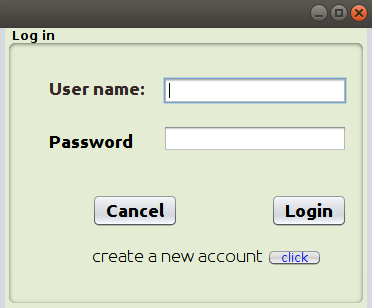
\includegraphics[height=5in]{/home/basedul/Documents/Report-writing-using-latex/ResturentManagementSystemReport/signin.png}
		\caption{Design for Signin}
		\label{fig:signout} 
\end{figure}

	\begin{lstlisting}
/*
 * To change this license header, choose License Headers in Project Properties.
 * To change this template file, choose Tools | Templates
 * and open the template in the editor.
 */
package RegistrationPackage;

import DatabaseConnection.DatabaseConnection;
import HomeActivity.MainActivity;
import RegistrationPackage.Admin.SignInClassForAdmin;
import static RegistrationPackage.Admin.SignInClassForAdmin.user_n;
import java.sql.PreparedStatement;
import java.sql.ResultSet;
import java.sql.SQLException;
import java.util.logging.Level;
import java.util.logging.Logger;
import javax.swing.JFrame;
import javax.swing.JOptionPane;

public class SignInClass extends javax.swing.JFrame {

    /**
     * Creates new form SignInClass
     * 
     * 
     */
    
    public static boolean checkUserIsEnable = false;
    public static String user_nc = "";
    
    public SignInClass() {
        initComponents();
    }
    
    public static void setCheck(boolean b) {
        checkUserIsEnable = !b;
    }
    
    public void loginStatusUpdate(String u_name) {
        PreparedStatement psForStatusUpdate;
        
        user_nc = u_name;
        
        String queryForUpdate = "UPDATE `Registration` SET `status`= ? WHERE `u_u_name`= ?";
        
        try {
            psForStatusUpdate = DatabaseConnection.getConnection().prepareStatement(queryForUpdate);
            psForStatusUpdate.setInt(1, 1);
            psForStatusUpdate.setString(2, u_name);
            psForStatusUpdate.executeUpdate();
        } catch (SQLException ex) {
            Logger.getLogger(SignInClassForAdmin.class.getName()).log(Level.SEVERE, null, ex);
        }
               
    }
    
    public void loginInfor() {
        PreparedStatement ps;
        ResultSet resultSet;

        String u_name = userNameFieldForLoginForm.getText();
        String u_pass = String.valueOf(passwordInLoginForm.getPassword());

        if (!u_name.equals("")) {

            //boolean exist = new RegisterForm().checkName(u_name);
            if (new SignUpClass().checkName(u_name)) {
                if (!u_pass.equals("")) {
                    String query = "SELECT * FROM `Registration` WHERE `u_u_name` =? AND `u_r_pass`=?";

                    try {
                        ps = DatabaseConnection.getConnection().prepareStatement(query);
                        ps.setString(1, u_name);
                        ps.setString(2, u_pass);

                        resultSet = ps.executeQuery();
                        if (resultSet.next()) {
                            
                            loginStatusUpdate(u_name);
                            
                            MainActivity mainActivity = new MainActivity();
                            mainActivity.setVisible(true);
                            mainActivity.setLocationRelativeTo(null);
                            mainActivity.setDefaultCloseOperation(JFrame.EXIT_ON_CLOSE);
                            this.dispose();
                            
                        } else {
                            JOptionPane.showMessageDialog(rootPane, "Enter correct infromation");
                        }

                    } catch (SQLException ex) {
                        Logger.getLogger(SignInClass.class.getName()).log(Level.SEVERE, null, ex);
                    }
                } else {
                    JOptionPane.showMessageDialog(rootPane, "Enter password");
                    passwordInLoginForm.requestFocus();
                }
            }else{
                JOptionPane.showMessageDialog(rootPane, "You have no account, please create an account!");
            }

        } else {
            JOptionPane.showMessageDialog(rootPane, "Enter user name");
            userNameFieldForLoginForm.requestFocus();
        }
    }

    /**
     * This method is called from within the constructor to initialize the form.
     * WARNING: Do NOT modify this code. The content of this method is always
     * regenerated by the Form Editor.
     */
    @SuppressWarnings("unchecked")
    // <editor-fold defaultstate="collapsed" desc="Generated Code">                          
    private void initComponents() {

        jPanel1 = new javax.swing.JPanel();
        UserNameLabel = new javax.swing.JLabel();
        PasswordLabel = new javax.swing.JLabel();
        userNameFieldForLoginForm = new javax.swing.JTextField();
        loginButton = new javax.swing.JButton();
        CancelButtonOnLoginForm = new javax.swing.JButton();
        jLabel1 = new javax.swing.JLabel();
        clickButtonOnLoginForm = new javax.swing.JButton();
        passwordInLoginForm = new javax.swing.JPasswordField();

        setDefaultCloseOperation(javax.swing.WindowConstants.EXIT_ON_CLOSE);

        jPanel1.setBackground(new java.awt.Color(228, 236, 211));
        jPanel1.setBorder(javax.swing.BorderFactory.createTitledBorder(javax.swing.BorderFactory.createTitledBorder("Log in")));

        UserNameLabel.setFont(new java.awt.Font("Ubuntu", 1, 18)); // NOI18N
        UserNameLabel.setForeground(new java.awt.Color(53, 39, 39));
        UserNameLabel.setText("User name:");
        UserNameLabel.setVerticalAlignment(javax.swing.SwingConstants.TOP);
        UserNameLabel.setAutoscrolls(true);

        PasswordLabel.setBackground(new java.awt.Color(24, 17, 9));
        PasswordLabel.setFont(new java.awt.Font("Ubuntu", 1, 18)); // NOI18N
        PasswordLabel.setText("Password");

        userNameFieldForLoginForm.setToolTipText("Enter your name");

        loginButton.setFont(new java.awt.Font("Ubuntu", 1, 18)); // NOI18N
        loginButton.setText("Login");
        loginButton.addActionListener(new java.awt.event.ActionListener() {
            public void actionPerformed(java.awt.event.ActionEvent evt) {
                loginButtonActionPerformed(evt);
            }
        });

        CancelButtonOnLoginForm.setFont(new java.awt.Font("Ubuntu", 1, 18)); // NOI18N
        CancelButtonOnLoginForm.setText("Cancel");
        CancelButtonOnLoginForm.addActionListener(new java.awt.event.ActionListener() {
            public void actionPerformed(java.awt.event.ActionEvent evt) {
                CancelButtonOnLoginFormActionPerformed(evt);
            }
        });

        jLabel1.setFont(new java.awt.Font("Ubuntu", 0, 18)); // NOI18N
        jLabel1.setText("create a new account");

        clickButtonOnLoginForm.setBackground(new java.awt.Color(174, 174, 174));
        clickButtonOnLoginForm.setForeground(new java.awt.Color(15, 33, 245));
        clickButtonOnLoginForm.setText("click");
        clickButtonOnLoginForm.addActionListener(new java.awt.event.ActionListener() {
            public void actionPerformed(java.awt.event.ActionEvent evt) {
                clickButtonOnLoginFormActionPerformed(evt);
            }
        });

        javax.swing.GroupLayout jPanel1Layout = new javax.swing.GroupLayout(jPanel1);
        jPanel1.setLayout(jPanel1Layout);
        jPanel1Layout.setHorizontalGroup(
            jPanel1Layout.createParallelGroup(javax.swing.GroupLayout.Alignment.LEADING)
            .addGroup(jPanel1Layout.createSequentialGroup()
                .addGroup(jPanel1Layout.createParallelGroup(javax.swing.GroupLayout.Alignment.TRAILING, false)
                    .addGroup(jPanel1Layout.createSequentialGroup()
                        .addContainerGap()
                        .addGroup(jPanel1Layout.createParallelGroup(javax.swing.GroupLayout.Alignment.LEADING, false)
                            .addComponent(UserNameLabel, javax.swing.GroupLayout.DEFAULT_SIZE, javax.swing.GroupLayout.DEFAULT_SIZE, Short.MAX_VALUE)
                            .addComponent(PasswordLabel, javax.swing.GroupLayout.DEFAULT_SIZE, javax.swing.GroupLayout.DEFAULT_SIZE, Short.MAX_VALUE))
                        .addGap(18, 18, 18)
                        .addGroup(jPanel1Layout.createParallelGroup(javax.swing.GroupLayout.Alignment.LEADING, false)
                            .addComponent(userNameFieldForLoginForm, javax.swing.GroupLayout.DEFAULT_SIZE, 184, Short.MAX_VALUE)
                            .addComponent(passwordInLoginForm)))
                    .addGroup(javax.swing.GroupLayout.Alignment.LEADING, jPanel1Layout.createSequentialGroup()
                        .addGap(73, 73, 73)
                        .addGroup(jPanel1Layout.createParallelGroup(javax.swing.GroupLayout.Alignment.LEADING)
                            .addGroup(jPanel1Layout.createSequentialGroup()
                                .addComponent(CancelButtonOnLoginForm)
                                .addPreferredGap(javax.swing.LayoutStyle.ComponentPlacement.RELATED, javax.swing.GroupLayout.DEFAULT_SIZE, Short.MAX_VALUE)
                                .addComponent(loginButton))
                            .addGroup(jPanel1Layout.createSequentialGroup()
                                .addComponent(jLabel1)
                                .addGap(4, 4, 4)
                                .addComponent(clickButtonOnLoginForm)
                                .addGap(0, 25, Short.MAX_VALUE)))))
                .addContainerGap(javax.swing.GroupLayout.DEFAULT_SIZE, Short.MAX_VALUE))
        );
        jPanel1Layout.setVerticalGroup(
            jPanel1Layout.createParallelGroup(javax.swing.GroupLayout.Alignment.LEADING)
            .addGroup(jPanel1Layout.createSequentialGroup()
                .addGap(22, 22, 22)
                .addGroup(jPanel1Layout.createParallelGroup(javax.swing.GroupLayout.Alignment.BASELINE)
                    .addComponent(UserNameLabel, javax.swing.GroupLayout.PREFERRED_SIZE, 25, javax.swing.GroupLayout.PREFERRED_SIZE)
                    .addComponent(userNameFieldForLoginForm, javax.swing.GroupLayout.PREFERRED_SIZE, javax.swing.GroupLayout.DEFAULT_SIZE, javax.swing.GroupLayout.PREFERRED_SIZE))
                .addGroup(jPanel1Layout.createParallelGroup(javax.swing.GroupLayout.Alignment.LEADING)
                    .addGroup(jPanel1Layout.createSequentialGroup()
                        .addGap(27, 27, 27)
                        .addComponent(PasswordLabel))
                    .addGroup(javax.swing.GroupLayout.Alignment.TRAILING, jPanel1Layout.createSequentialGroup()
                        .addGap(21, 21, 21)
                        .addComponent(passwordInLoginForm, javax.swing.GroupLayout.PREFERRED_SIZE, 27, javax.swing.GroupLayout.PREFERRED_SIZE)))
                .addGap(42, 42, 42)
                .addGroup(jPanel1Layout.createParallelGroup(javax.swing.GroupLayout.Alignment.BASELINE)
                    .addComponent(loginButton)
                    .addComponent(CancelButtonOnLoginForm))
                .addGap(18, 18, 18)
                .addGroup(jPanel1Layout.createParallelGroup(javax.swing.GroupLayout.Alignment.BASELINE)
                    .addComponent(jLabel1)
                    .addComponent(clickButtonOnLoginForm, javax.swing.GroupLayout.PREFERRED_SIZE, 17, javax.swing.GroupLayout.PREFERRED_SIZE))
                .addContainerGap(29, Short.MAX_VALUE))
        );

        javax.swing.GroupLayout layout = new javax.swing.GroupLayout(getContentPane());
        getContentPane().setLayout(layout);
        layout.setHorizontalGroup(
            layout.createParallelGroup(javax.swing.GroupLayout.Alignment.LEADING)
            .addGroup(javax.swing.GroupLayout.Alignment.TRAILING, layout.createSequentialGroup()
                .addContainerGap(javax.swing.GroupLayout.DEFAULT_SIZE, Short.MAX_VALUE)
                .addComponent(jPanel1, javax.swing.GroupLayout.PREFERRED_SIZE, javax.swing.GroupLayout.DEFAULT_SIZE, javax.swing.GroupLayout.PREFERRED_SIZE)
                .addContainerGap())
        );
        layout.setVerticalGroup(
            layout.createParallelGroup(javax.swing.GroupLayout.Alignment.LEADING)
            .addGroup(javax.swing.GroupLayout.Alignment.TRAILING, layout.createSequentialGroup()
                .addGap(0, 0, Short.MAX_VALUE)
                .addComponent(jPanel1, javax.swing.GroupLayout.PREFERRED_SIZE, javax.swing.GroupLayout.DEFAULT_SIZE, javax.swing.GroupLayout.PREFERRED_SIZE))
        );

        pack();
    }// </editor-fold>                        

    private void loginButtonActionPerformed(java.awt.event.ActionEvent evt) {                                            
        loginInfor();
    }                                           

    private void CancelButtonOnLoginFormActionPerformed(java.awt.event.ActionEvent evt) {                                                        
        MainActivity mainActivity = new MainActivity();
        mainActivity.setVisible(true);
        mainActivity.setLocationRelativeTo(null);
        mainActivity.setDefaultCloseOperation(JFrame.EXIT_ON_CLOSE);
        this.dispose();
    }                                                       

    private void clickButtonOnLoginFormActionPerformed(java.awt.event.ActionEvent evt) {                                                       
        SignUpClass registerForm = new SignUpClass();
        registerForm.setVisible(true);
        registerForm.setLocationRelativeTo(null);
        registerForm.setDefaultCloseOperation(JFrame.EXIT_ON_CLOSE);
        this.dispose();
    }                                                      

    /**
     * @param args the command line arguments
     */
    public static void main(String args[]) {
        /* Set the Nimbus look and feel */
        //<editor-fold defaultstate="collapsed" desc=" Look and feel setting code (optional) ">
        /* If Nimbus (introduced in Java SE 6) is not available, stay with the default look and feel.
         * For details see http://download.oracle.com/javase/tutorial/uiswing/lookandfeel/plaf.html 
         */
        try {
            for (javax.swing.UIManager.LookAndFeelInfo info : javax.swing.UIManager.getInstalledLookAndFeels()) {
                if ("Nimbus".equals(info.getName())) {
                    javax.swing.UIManager.setLookAndFeel(info.getClassName());
                    break;
                }
            }
        } catch (ClassNotFoundException ex) {
            java.util.logging.Logger.getLogger(SignInClass.class.getName()).log(java.util.logging.Level.SEVERE, null, ex);
        } catch (InstantiationException ex) {
            java.util.logging.Logger.getLogger(SignInClass.class.getName()).log(java.util.logging.Level.SEVERE, null, ex);
        } catch (IllegalAccessException ex) {
            java.util.logging.Logger.getLogger(SignInClass.class.getName()).log(java.util.logging.Level.SEVERE, null, ex);
        } catch (javax.swing.UnsupportedLookAndFeelException ex) {
            java.util.logging.Logger.getLogger(SignInClass.class.getName()).log(java.util.logging.Level.SEVERE, null, ex);
        }
        //</editor-fold>

        /* Create and display the form */
        java.awt.EventQueue.invokeLater(new Runnable() {
            public void run() {
                new SignInClass().setVisible(true);
            }
        });
    }
    
    // Variables declaration - do not modify                     
    private javax.swing.JButton CancelButtonOnLoginForm;
    private javax.swing.JLabel PasswordLabel;
    private javax.swing.JLabel UserNameLabel;
    private javax.swing.JButton clickButtonOnLoginForm;
    private javax.swing.JLabel jLabel1;
    private javax.swing.JPanel jPanel1;
    private javax.swing.JButton loginButton;
    private javax.swing.JPasswordField passwordInLoginForm;
    private javax.swing.JTextField userNameFieldForLoginForm;
    // End of variables declaration                   
}

	\end{lstlisting}
	
	\subsubsection{Sign UP}
		\begin{figure}[H]
		\centering
		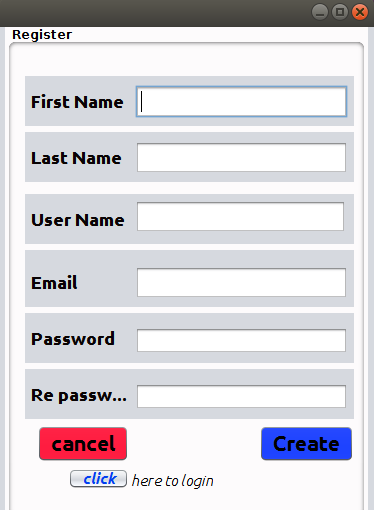
\includegraphics[height=5in]{/home/basedul/Documents/Report-writing-using-latex/ResturentManagementSystemReport/signup.png}
		\caption{Design for Sign up}
		\label{fig:signin} 
\end{figure}
	\begin{lstlisting}
		/*
 * To change this license header, choose License Headers in Project Properties.
 * To change this template file, choose Tools | Templates
 * and open the template in the editor.
 */
package RegistrationPackage;

import DatabaseConnection.DatabaseConnection;
import HomeActivity.MainActivity;
import java.sql.PreparedStatement;
import java.sql.ResultSet;
import java.sql.SQLException;
import java.util.logging.Level;
import java.util.logging.Logger;
import javax.swing.JFrame;
import javax.swing.JOptionPane;

/**
 *
 * @author basedul
 */
public class SignUpClass extends javax.swing.JFrame {

    /**
     * Creates new form SignUpClass
     */
    public SignUpClass() {
        initComponents();
        setLocationRelativeTo(null);
    }
    
    public boolean checkName(String name) {
        boolean checkN = false;

        PreparedStatement ps;
        ResultSet rs;
        String query = "SELECT * FROM `Registration` WHERE `u_u_name` =?";

        try {
            ps = DatabaseConnection.getConnection().prepareStatement(query);
            ps.setString(1, name);
            rs = ps.executeQuery();
            if (rs.next()) {
                checkN = true;
            }
        } catch (SQLException ex) {
            Logger.getLogger(SignUpClass.class.getName()).log(Level.SEVERE, null, ex);
        }

        return checkN;
    }

    /**
     * This method is called from within the constructor to initialize the form.
     * WARNING: Do NOT modify this code. The content of this method is always
     * regenerated by the Form Editor.
     */
    @SuppressWarnings("unchecked")
    // <editor-fold defaultstate="collapsed" desc="Generated Code">                          
    private void initComponents() {

        jPanel1 = new javax.swing.JPanel();
        jPanel2 = new javax.swing.JPanel();
        jLabel1 = new javax.swing.JLabel();
        firstNameTextFieldInRegisterForm = new javax.swing.JTextField();
        jPanel3 = new javax.swing.JPanel();
        jLabel2 = new javax.swing.JLabel();
        lastNameTextFieldInRegisterForm = new javax.swing.JTextField();
        jPanel4 = new javax.swing.JPanel();
        jLabel4 = new javax.swing.JLabel();
        jPasswordFieldinRegistrationForm = new javax.swing.JPasswordField();
        jPanel5 = new javax.swing.JPanel();
        jLabel3 = new javax.swing.JLabel();
        userNameTextFieldInRegisterForm = new javax.swing.JTextField();
        jPanel6 = new javax.swing.JPanel();
        jLabel5 = new javax.swing.JLabel();
        jPasswordField2inRegistrationFrom = new javax.swing.JPasswordField();
        jPanel8 = new javax.swing.JPanel();
        jLabel7 = new javax.swing.JLabel();
        emailTextFieldInRegisterForm = new javax.swing.JTextField();
        CreateButtonInRegistrationForm = new javax.swing.JButton();
        cancellButtonInRegistrationForm = new javax.swing.JButton();
        jLabel9 = new javax.swing.JLabel();
        clickHereToLoginButtonOnRegistrationButton = new javax.swing.JButton();

        setDefaultCloseOperation(javax.swing.WindowConstants.EXIT_ON_CLOSE);

        jPanel1.setBackground(new java.awt.Color(253, 251, 252));
        jPanel1.setBorder(javax.swing.BorderFactory.createTitledBorder("Register"));
        jPanel1.setForeground(new java.awt.Color(254, 254, 254));

        jLabel1.setBackground(new java.awt.Color(7, 7, 7));
        jLabel1.setFont(new java.awt.Font("Ubuntu", 1, 18)); // NOI18N
        jLabel1.setForeground(new java.awt.Color(9, 4, 4));
        jLabel1.setText("First Name");

        firstNameTextFieldInRegisterForm.setFont(new java.awt.Font("Ubuntu", 0, 18)); // NOI18N

        javax.swing.GroupLayout jPanel2Layout = new javax.swing.GroupLayout(jPanel2);
        jPanel2.setLayout(jPanel2Layout);
        jPanel2Layout.setHorizontalGroup(
            jPanel2Layout.createParallelGroup(javax.swing.GroupLayout.Alignment.LEADING)
            .addGroup(jPanel2Layout.createSequentialGroup()
                .addContainerGap()
                .addComponent(jLabel1, javax.swing.GroupLayout.PREFERRED_SIZE, 98, javax.swing.GroupLayout.PREFERRED_SIZE)
                .addPreferredGap(javax.swing.LayoutStyle.ComponentPlacement.RELATED)
                .addComponent(firstNameTextFieldInRegisterForm, javax.swing.GroupLayout.PREFERRED_SIZE, 213, javax.swing.GroupLayout.PREFERRED_SIZE)
                .addContainerGap(javax.swing.GroupLayout.DEFAULT_SIZE, Short.MAX_VALUE))
        );
        jPanel2Layout.setVerticalGroup(
            jPanel2Layout.createParallelGroup(javax.swing.GroupLayout.Alignment.LEADING)
            .addGroup(jPanel2Layout.createSequentialGroup()
                .addContainerGap()
                .addGroup(jPanel2Layout.createParallelGroup(javax.swing.GroupLayout.Alignment.BASELINE)
                    .addComponent(jLabel1, javax.swing.GroupLayout.PREFERRED_SIZE, 38, javax.swing.GroupLayout.PREFERRED_SIZE)
                    .addComponent(firstNameTextFieldInRegisterForm, javax.swing.GroupLayout.PREFERRED_SIZE, javax.swing.GroupLayout.DEFAULT_SIZE, javax.swing.GroupLayout.PREFERRED_SIZE))
                .addContainerGap(javax.swing.GroupLayout.DEFAULT_SIZE, Short.MAX_VALUE))
        );

        jLabel2.setBackground(new java.awt.Color(7, 7, 7));
        jLabel2.setFont(new java.awt.Font("Ubuntu", 1, 18)); // NOI18N
        jLabel2.setForeground(new java.awt.Color(9, 4, 4));
        jLabel2.setText("Last Name");

        lastNameTextFieldInRegisterForm.setFont(new java.awt.Font("Ubuntu", 0, 18)); // NOI18N

        javax.swing.GroupLayout jPanel3Layout = new javax.swing.GroupLayout(jPanel3);
        jPanel3.setLayout(jPanel3Layout);
        jPanel3Layout.setHorizontalGroup(
            jPanel3Layout.createParallelGroup(javax.swing.GroupLayout.Alignment.LEADING)
            .addGroup(jPanel3Layout.createSequentialGroup()
                .addContainerGap()
                .addComponent(jLabel2, javax.swing.GroupLayout.PREFERRED_SIZE, 98, javax.swing.GroupLayout.PREFERRED_SIZE)
                .addPreferredGap(javax.swing.LayoutStyle.ComponentPlacement.RELATED)
                .addComponent(lastNameTextFieldInRegisterForm, javax.swing.GroupLayout.PREFERRED_SIZE, 213, javax.swing.GroupLayout.PREFERRED_SIZE)
                .addContainerGap(javax.swing.GroupLayout.DEFAULT_SIZE, Short.MAX_VALUE))
        );
        jPanel3Layout.setVerticalGroup(
            jPanel3Layout.createParallelGroup(javax.swing.GroupLayout.Alignment.LEADING)
            .addGroup(jPanel3Layout.createSequentialGroup()
                .addContainerGap()
                .addGroup(jPanel3Layout.createParallelGroup(javax.swing.GroupLayout.Alignment.BASELINE)
                    .addComponent(jLabel2, javax.swing.GroupLayout.PREFERRED_SIZE, 38, javax.swing.GroupLayout.PREFERRED_SIZE)
                    .addComponent(lastNameTextFieldInRegisterForm, javax.swing.GroupLayout.PREFERRED_SIZE, javax.swing.GroupLayout.DEFAULT_SIZE, javax.swing.GroupLayout.PREFERRED_SIZE))
                .addContainerGap(javax.swing.GroupLayout.DEFAULT_SIZE, Short.MAX_VALUE))
        );

        jLabel4.setBackground(new java.awt.Color(7, 7, 7));
        jLabel4.setFont(new java.awt.Font("Ubuntu", 1, 18)); // NOI18N
        jLabel4.setForeground(new java.awt.Color(9, 4, 4));
        jLabel4.setText("Password");

        jPasswordFieldinRegistrationForm.addActionListener(new java.awt.event.ActionListener() {
            public void actionPerformed(java.awt.event.ActionEvent evt) {
                jPasswordFieldinRegistrationFormActionPerformed(evt);
            }
        });

        javax.swing.GroupLayout jPanel4Layout = new javax.swing.GroupLayout(jPanel4);
        jPanel4.setLayout(jPanel4Layout);
        jPanel4Layout.setHorizontalGroup(
            jPanel4Layout.createParallelGroup(javax.swing.GroupLayout.Alignment.LEADING)
            .addGroup(jPanel4Layout.createSequentialGroup()
                .addContainerGap()
                .addComponent(jLabel4, javax.swing.GroupLayout.PREFERRED_SIZE, 98, javax.swing.GroupLayout.PREFERRED_SIZE)
                .addPreferredGap(javax.swing.LayoutStyle.ComponentPlacement.RELATED)
                .addComponent(jPasswordFieldinRegistrationForm)
                .addContainerGap())
        );
        jPanel4Layout.setVerticalGroup(
            jPanel4Layout.createParallelGroup(javax.swing.GroupLayout.Alignment.LEADING)
            .addGroup(jPanel4Layout.createSequentialGroup()
                .addContainerGap()
                .addGroup(jPanel4Layout.createParallelGroup(javax.swing.GroupLayout.Alignment.BASELINE)
                    .addComponent(jLabel4, javax.swing.GroupLayout.PREFERRED_SIZE, 38, javax.swing.GroupLayout.PREFERRED_SIZE)
                    .addComponent(jPasswordFieldinRegistrationForm, javax.swing.GroupLayout.PREFERRED_SIZE, javax.swing.GroupLayout.DEFAULT_SIZE, javax.swing.GroupLayout.PREFERRED_SIZE))
                .addContainerGap(javax.swing.GroupLayout.DEFAULT_SIZE, Short.MAX_VALUE))
        );

        jLabel3.setBackground(new java.awt.Color(7, 7, 7));
        jLabel3.setFont(new java.awt.Font("Ubuntu", 1, 18)); // NOI18N
        jLabel3.setForeground(new java.awt.Color(9, 4, 4));
        jLabel3.setText("User Name");

        userNameTextFieldInRegisterForm.setFont(new java.awt.Font("Ubuntu", 0, 18)); // NOI18N

        javax.swing.GroupLayout jPanel5Layout = new javax.swing.GroupLayout(jPanel5);
        jPanel5.setLayout(jPanel5Layout);
        jPanel5Layout.setHorizontalGroup(
            jPanel5Layout.createParallelGroup(javax.swing.GroupLayout.Alignment.LEADING)
            .addGroup(jPanel5Layout.createSequentialGroup()
                .addContainerGap()
                .addComponent(jLabel3, javax.swing.GroupLayout.PREFERRED_SIZE, 98, javax.swing.GroupLayout.PREFERRED_SIZE)
                .addPreferredGap(javax.swing.LayoutStyle.ComponentPlacement.RELATED)
                .addComponent(userNameTextFieldInRegisterForm, javax.swing.GroupLayout.PREFERRED_SIZE, 211, javax.swing.GroupLayout.PREFERRED_SIZE)
                .addContainerGap(javax.swing.GroupLayout.DEFAULT_SIZE, Short.MAX_VALUE))
        );
        jPanel5Layout.setVerticalGroup(
            jPanel5Layout.createParallelGroup(javax.swing.GroupLayout.Alignment.LEADING)
            .addGroup(jPanel5Layout.createSequentialGroup()
                .addContainerGap()
                .addGroup(jPanel5Layout.createParallelGroup(javax.swing.GroupLayout.Alignment.LEADING)
                    .addComponent(userNameTextFieldInRegisterForm, javax.swing.GroupLayout.PREFERRED_SIZE, javax.swing.GroupLayout.DEFAULT_SIZE, javax.swing.GroupLayout.PREFERRED_SIZE)
                    .addComponent(jLabel3, javax.swing.GroupLayout.PREFERRED_SIZE, 38, javax.swing.GroupLayout.PREFERRED_SIZE))
                .addContainerGap(javax.swing.GroupLayout.DEFAULT_SIZE, Short.MAX_VALUE))
        );

        jLabel5.setBackground(new java.awt.Color(7, 7, 7));
        jLabel5.setFont(new java.awt.Font("Ubuntu", 1, 18)); // NOI18N
        jLabel5.setForeground(new java.awt.Color(9, 4, 4));
        jLabel5.setText("Re password");

        javax.swing.GroupLayout jPanel6Layout = new javax.swing.GroupLayout(jPanel6);
        jPanel6.setLayout(jPanel6Layout);
        jPanel6Layout.setHorizontalGroup(
            jPanel6Layout.createParallelGroup(javax.swing.GroupLayout.Alignment.LEADING)
            .addGroup(javax.swing.GroupLayout.Alignment.TRAILING, jPanel6Layout.createSequentialGroup()
                .addContainerGap()
                .addComponent(jLabel5, javax.swing.GroupLayout.PREFERRED_SIZE, 98, javax.swing.GroupLayout.PREFERRED_SIZE)
                .addPreferredGap(javax.swing.LayoutStyle.ComponentPlacement.RELATED)
                .addComponent(jPasswordField2inRegistrationFrom)
                .addContainerGap())
        );
        jPanel6Layout.setVerticalGroup(
            jPanel6Layout.createParallelGroup(javax.swing.GroupLayout.Alignment.LEADING)
            .addGroup(jPanel6Layout.createSequentialGroup()
                .addContainerGap()
                .addGroup(jPanel6Layout.createParallelGroup(javax.swing.GroupLayout.Alignment.BASELINE)
                    .addComponent(jLabel5, javax.swing.GroupLayout.PREFERRED_SIZE, 38, javax.swing.GroupLayout.PREFERRED_SIZE)
                    .addComponent(jPasswordField2inRegistrationFrom, javax.swing.GroupLayout.PREFERRED_SIZE, javax.swing.GroupLayout.DEFAULT_SIZE, javax.swing.GroupLayout.PREFERRED_SIZE))
                .addContainerGap(javax.swing.GroupLayout.DEFAULT_SIZE, Short.MAX_VALUE))
        );

        jLabel7.setBackground(new java.awt.Color(7, 7, 7));
        jLabel7.setFont(new java.awt.Font("Ubuntu", 1, 18)); // NOI18N
        jLabel7.setForeground(new java.awt.Color(9, 4, 4));
        jLabel7.setText("Email");

        emailTextFieldInRegisterForm.setFont(new java.awt.Font("Ubuntu", 0, 18)); // NOI18N

        javax.swing.GroupLayout jPanel8Layout = new javax.swing.GroupLayout(jPanel8);
        jPanel8.setLayout(jPanel8Layout);
        jPanel8Layout.setHorizontalGroup(
            jPanel8Layout.createParallelGroup(javax.swing.GroupLayout.Alignment.LEADING)
            .addGroup(jPanel8Layout.createSequentialGroup()
                .addContainerGap()
                .addComponent(jLabel7, javax.swing.GroupLayout.PREFERRED_SIZE, 61, javax.swing.GroupLayout.PREFERRED_SIZE)
                .addPreferredGap(javax.swing.LayoutStyle.ComponentPlacement.RELATED, javax.swing.GroupLayout.DEFAULT_SIZE, Short.MAX_VALUE)
                .addComponent(emailTextFieldInRegisterForm, javax.swing.GroupLayout.PREFERRED_SIZE, 213, javax.swing.GroupLayout.PREFERRED_SIZE)
                .addContainerGap())
        );
        jPanel8Layout.setVerticalGroup(
            jPanel8Layout.createParallelGroup(javax.swing.GroupLayout.Alignment.LEADING)
            .addGroup(javax.swing.GroupLayout.Alignment.TRAILING, jPanel8Layout.createSequentialGroup()
                .addContainerGap(13, Short.MAX_VALUE)
                .addGroup(jPanel8Layout.createParallelGroup(javax.swing.GroupLayout.Alignment.BASELINE)
                    .addComponent(jLabel7, javax.swing.GroupLayout.PREFERRED_SIZE, 38, javax.swing.GroupLayout.PREFERRED_SIZE)
                    .addComponent(emailTextFieldInRegisterForm))
                .addContainerGap())
        );

        CreateButtonInRegistrationForm.setBackground(new java.awt.Color(11, 48, 242));
        CreateButtonInRegistrationForm.setFont(new java.awt.Font("Ubuntu", 1, 21)); // NOI18N
        CreateButtonInRegistrationForm.setText("Create");
        CreateButtonInRegistrationForm.addActionListener(new java.awt.event.ActionListener() {
            public void actionPerformed(java.awt.event.ActionEvent evt) {
                CreateButtonInRegistrationFormActionPerformed(evt);
            }
        });

        cancellButtonInRegistrationForm.setBackground(new java.awt.Color(244, 9, 46));
        cancellButtonInRegistrationForm.setFont(new java.awt.Font("Ubuntu", 1, 21)); // NOI18N
        cancellButtonInRegistrationForm.setText("cancel");
        cancellButtonInRegistrationForm.addActionListener(new java.awt.event.ActionListener() {
            public void actionPerformed(java.awt.event.ActionEvent evt) {
                cancellButtonInRegistrationFormActionPerformed(evt);
            }
        });

        jLabel9.setFont(new java.awt.Font("Ubuntu", 2, 15)); // NOI18N
        jLabel9.setText("here to login");

        clickHereToLoginButtonOnRegistrationButton.setFont(new java.awt.Font("Ubuntu", 3, 15)); // NOI18N
        clickHereToLoginButtonOnRegistrationButton.setForeground(new java.awt.Color(2, 62, 241));
        clickHereToLoginButtonOnRegistrationButton.setText("click");
        clickHereToLoginButtonOnRegistrationButton.addActionListener(new java.awt.event.ActionListener() {
            public void actionPerformed(java.awt.event.ActionEvent evt) {
                clickHereToLoginButtonOnRegistrationButtonActionPerformed(evt);
            }
        });

        javax.swing.GroupLayout jPanel1Layout = new javax.swing.GroupLayout(jPanel1);
        jPanel1.setLayout(jPanel1Layout);
        jPanel1Layout.setHorizontalGroup(
            jPanel1Layout.createParallelGroup(javax.swing.GroupLayout.Alignment.LEADING)
            .addGroup(jPanel1Layout.createSequentialGroup()
                .addContainerGap()
                .addGroup(jPanel1Layout.createParallelGroup(javax.swing.GroupLayout.Alignment.LEADING)
                    .addComponent(jPanel8, javax.swing.GroupLayout.Alignment.TRAILING, javax.swing.GroupLayout.DEFAULT_SIZE, javax.swing.GroupLayout.DEFAULT_SIZE, Short.MAX_VALUE)
                    .addGroup(jPanel1Layout.createSequentialGroup()
                        .addGroup(jPanel1Layout.createParallelGroup(javax.swing.GroupLayout.Alignment.LEADING, false)
                            .addComponent(jPanel4, javax.swing.GroupLayout.DEFAULT_SIZE, javax.swing.GroupLayout.DEFAULT_SIZE, Short.MAX_VALUE)
                            .addComponent(jPanel5, javax.swing.GroupLayout.DEFAULT_SIZE, javax.swing.GroupLayout.DEFAULT_SIZE, Short.MAX_VALUE)
                            .addComponent(jPanel3, javax.swing.GroupLayout.DEFAULT_SIZE, javax.swing.GroupLayout.DEFAULT_SIZE, Short.MAX_VALUE)
                            .addComponent(jPanel2, javax.swing.GroupLayout.DEFAULT_SIZE, javax.swing.GroupLayout.DEFAULT_SIZE, Short.MAX_VALUE)
                            .addComponent(jPanel6, javax.swing.GroupLayout.DEFAULT_SIZE, javax.swing.GroupLayout.DEFAULT_SIZE, Short.MAX_VALUE))
                        .addGap(0, 0, Short.MAX_VALUE))
                    .addGroup(jPanel1Layout.createSequentialGroup()
                        .addGap(12, 12, 12)
                        .addGroup(jPanel1Layout.createParallelGroup(javax.swing.GroupLayout.Alignment.TRAILING)
                            .addComponent(clickHereToLoginButtonOnRegistrationButton)
                            .addComponent(cancellButtonInRegistrationForm))
                        .addGroup(jPanel1Layout.createParallelGroup(javax.swing.GroupLayout.Alignment.LEADING)
                            .addGroup(jPanel1Layout.createSequentialGroup()
                                .addPreferredGap(javax.swing.LayoutStyle.ComponentPlacement.RELATED, javax.swing.GroupLayout.DEFAULT_SIZE, Short.MAX_VALUE)
                                .addComponent(CreateButtonInRegistrationForm, javax.swing.GroupLayout.PREFERRED_SIZE, 95, javax.swing.GroupLayout.PREFERRED_SIZE))
                            .addGroup(jPanel1Layout.createSequentialGroup()
                                .addGap(2, 2, 2)
                                .addComponent(jLabel9)))))
                .addContainerGap())
        );
        jPanel1Layout.setVerticalGroup(
            jPanel1Layout.createParallelGroup(javax.swing.GroupLayout.Alignment.LEADING)
            .addGroup(jPanel1Layout.createSequentialGroup()
                .addGap(22, 22, 22)
                .addComponent(jPanel2, javax.swing.GroupLayout.PREFERRED_SIZE, javax.swing.GroupLayout.DEFAULT_SIZE, javax.swing.GroupLayout.PREFERRED_SIZE)
                .addPreferredGap(javax.swing.LayoutStyle.ComponentPlacement.RELATED)
                .addComponent(jPanel3, javax.swing.GroupLayout.PREFERRED_SIZE, javax.swing.GroupLayout.DEFAULT_SIZE, javax.swing.GroupLayout.PREFERRED_SIZE)
                .addPreferredGap(javax.swing.LayoutStyle.ComponentPlacement.UNRELATED)
                .addComponent(jPanel5, javax.swing.GroupLayout.PREFERRED_SIZE, javax.swing.GroupLayout.DEFAULT_SIZE, javax.swing.GroupLayout.PREFERRED_SIZE)
                .addPreferredGap(javax.swing.LayoutStyle.ComponentPlacement.RELATED)
                .addComponent(jPanel8, javax.swing.GroupLayout.PREFERRED_SIZE, javax.swing.GroupLayout.DEFAULT_SIZE, javax.swing.GroupLayout.PREFERRED_SIZE)
                .addPreferredGap(javax.swing.LayoutStyle.ComponentPlacement.RELATED, javax.swing.GroupLayout.DEFAULT_SIZE, Short.MAX_VALUE)
                .addComponent(jPanel4, javax.swing.GroupLayout.PREFERRED_SIZE, javax.swing.GroupLayout.DEFAULT_SIZE, javax.swing.GroupLayout.PREFERRED_SIZE)
                .addPreferredGap(javax.swing.LayoutStyle.ComponentPlacement.RELATED)
                .addComponent(jPanel6, javax.swing.GroupLayout.PREFERRED_SIZE, javax.swing.GroupLayout.DEFAULT_SIZE, javax.swing.GroupLayout.PREFERRED_SIZE)
                .addPreferredGap(javax.swing.LayoutStyle.ComponentPlacement.RELATED)
                .addGroup(jPanel1Layout.createParallelGroup(javax.swing.GroupLayout.Alignment.LEADING, false)
                    .addComponent(cancellButtonInRegistrationForm, javax.swing.GroupLayout.DEFAULT_SIZE, javax.swing.GroupLayout.DEFAULT_SIZE, Short.MAX_VALUE)
                    .addComponent(CreateButtonInRegistrationForm, javax.swing.GroupLayout.DEFAULT_SIZE, javax.swing.GroupLayout.DEFAULT_SIZE, Short.MAX_VALUE))
                .addGroup(jPanel1Layout.createParallelGroup(javax.swing.GroupLayout.Alignment.LEADING, false)
                    .addGroup(jPanel1Layout.createSequentialGroup()
                        .addGap(9, 9, 9)
                        .addComponent(jLabel9))
                    .addGroup(jPanel1Layout.createSequentialGroup()
                        .addPreferredGap(javax.swing.LayoutStyle.ComponentPlacement.RELATED)
                        .addComponent(clickHereToLoginButtonOnRegistrationButton, javax.swing.GroupLayout.PREFERRED_SIZE, 0, Short.MAX_VALUE)))
                .addGap(18, 18, 18))
        );

        javax.swing.GroupLayout layout = new javax.swing.GroupLayout(getContentPane());
        getContentPane().setLayout(layout);
        layout.setHorizontalGroup(
            layout.createParallelGroup(javax.swing.GroupLayout.Alignment.LEADING)
            .addGroup(layout.createSequentialGroup()
                .addContainerGap()
                .addComponent(jPanel1, javax.swing.GroupLayout.PREFERRED_SIZE, 363, javax.swing.GroupLayout.PREFERRED_SIZE)
                .addContainerGap(javax.swing.GroupLayout.DEFAULT_SIZE, Short.MAX_VALUE))
        );
        layout.setVerticalGroup(
            layout.createParallelGroup(javax.swing.GroupLayout.Alignment.LEADING)
            .addGroup(javax.swing.GroupLayout.Alignment.TRAILING, layout.createSequentialGroup()
                .addComponent(jPanel1, javax.swing.GroupLayout.PREFERRED_SIZE, javax.swing.GroupLayout.DEFAULT_SIZE, javax.swing.GroupLayout.PREFERRED_SIZE)
                .addGap(0, 0, Short.MAX_VALUE))
        );

        pack();
    }// </editor-fold>                        

    private void jPasswordFieldinRegistrationFormActionPerformed(java.awt.event.ActionEvent evt) {                                                                 
        // TODO add your handling code here:
    }                                                                

    private void CreateButtonInRegistrationFormActionPerformed(java.awt.event.ActionEvent evt) {                                                               

        String firstName = firstNameTextFieldInRegisterForm.getText();
        String lastName = lastNameTextFieldInRegisterForm.getText();
        String UserName = userNameTextFieldInRegisterForm.getText();
        String Email = emailTextFieldInRegisterForm.getText();
        String Pass_01 = String.valueOf(jPasswordFieldinRegistrationForm.getPassword());
        String Pas_02 = String.valueOf(jPasswordField2inRegistrationFrom.getPassword());
        int status = 0;

        if (!firstName.equals("")) {

            if (!lastName.equals("")) {

                if (!UserName.equals("")) {

                    if (!Email.equals("")) {

                        if (!Pass_01.equals("")) {

                            if (Pas_02.equals(Pass_01)) {

                                if (checkName(UserName)) {
                                    JOptionPane.showMessageDialog(null, "User Name already exists !");
                                    jPasswordField2inRegistrationFrom.requestFocus();
                                } else {
                                    PreparedStatement ps;
                                    String query = "INSERT INTO `Registration`(`u_f_name`, `u_l_name`, `u_u_name`, `U_mail`, `u_f_pass`, `u_r_pass`, `status`, `reward_point`) VALUES (?,?,?,?,?,?,?,?)";

                                    try {

                                        ps = DatabaseConnection.getConnection().prepareStatement(query);

                                        ps.setString(1, firstName);
                                        ps.setString(2, lastName);
                                        ps.setString(3, UserName);
                                        ps.setString(4, Email);
                                        ps.setString(5, Pass_01);
                                        ps.setString(6, Pas_02);
                                        ps.setInt(7, status);
                                        ps.setFloat(8, 0);

                                        if (ps.executeUpdate() > 0) {
                                            JOptionPane.showMessageDialog(null, "New User Add");
                                            SignInClass loginForm = new SignInClass();
                                            loginForm.setVisible(true);
                                            loginForm.setLocationRelativeTo(null);
                                            loginForm.setDefaultCloseOperation(JFrame.EXIT_ON_CLOSE);
                                            dispose();
                                        }

                                    } catch (SQLException ex) {
                                        Logger.getLogger(SignUpClass.class.getName()).log(Level.SEVERE, null, ex);
                                    }
                                }

                            } else {
                                JOptionPane.showMessageDialog(null, "Password doesn't match");
                                jPasswordField2inRegistrationFrom.requestFocus();
                            }

                        } else {
                            JOptionPane.showMessageDialog(null, "Enter password");
                            jPasswordFieldinRegistrationForm.requestFocus();
                        }

                    } else {
                        JOptionPane.showMessageDialog(null, "Enter mail");
                        emailTextFieldInRegisterForm.requestFocus();
                    }

                } else {
                    JOptionPane.showMessageDialog(null, "Enter user name");
                    userNameTextFieldInRegisterForm.requestFocus();
                }
            } else {
                JOptionPane.showMessageDialog(null, "Enter last name");
                lastNameTextFieldInRegisterForm.requestFocus();
            }
        } else {
            JOptionPane.showMessageDialog(null, "Enter first name");
            firstNameTextFieldInRegisterForm.requestFocus();
        }
    }                                                              

    private void cancellButtonInRegistrationFormActionPerformed(java.awt.event.ActionEvent evt) {                                                                
        MainActivity mainActivity = new MainActivity();
        mainActivity.setVisible(true);
        mainActivity.setLocationRelativeTo(null);
        mainActivity.setDefaultCloseOperation(JFrame.EXIT_ON_CLOSE);
        this.dispose();
    }                                                               

    private void clickHereToLoginButtonOnRegistrationButtonActionPerformed(java.awt.event.ActionEvent evt) {                                                                           
        SignInClass loginForm = new SignInClass();
        loginForm.setVisible(true);
        loginForm.setLocationRelativeTo(null);
        loginForm.setDefaultCloseOperation(JFrame.EXIT_ON_CLOSE);
        this.dispose();
    }                                                                          

    /**
     * @param args the command line arguments
     */
    public static void main(String args[]) {
        /* Set the Nimbus look and feel */
        //<editor-fold defaultstate="collapsed" desc=" Look and feel setting code (optional) ">
        /* If Nimbus (introduced in Java SE 6) is not available, stay with the default look and feel.
         * For details see http://download.oracle.com/javase/tutorial/uiswing/lookandfeel/plaf.html 
         */
        try {
            for (javax.swing.UIManager.LookAndFeelInfo info : javax.swing.UIManager.getInstalledLookAndFeels()) {
                if ("Nimbus".equals(info.getName())) {
                    javax.swing.UIManager.setLookAndFeel(info.getClassName());
                    break;
                }
            }
        } catch (ClassNotFoundException ex) {
            java.util.logging.Logger.getLogger(SignUpClass.class.getName()).log(java.util.logging.Level.SEVERE, null, ex);
        } catch (InstantiationException ex) {
            java.util.logging.Logger.getLogger(SignUpClass.class.getName()).log(java.util.logging.Level.SEVERE, null, ex);
        } catch (IllegalAccessException ex) {
            java.util.logging.Logger.getLogger(SignUpClass.class.getName()).log(java.util.logging.Level.SEVERE, null, ex);
        } catch (javax.swing.UnsupportedLookAndFeelException ex) {
            java.util.logging.Logger.getLogger(SignUpClass.class.getName()).log(java.util.logging.Level.SEVERE, null, ex);
        }
        //</editor-fold>

        /* Create and display the form */
        java.awt.EventQueue.invokeLater(new Runnable() {
            public void run() {
                new SignUpClass().setVisible(true);
            }
        });
    }

    // Variables declaration - do not modify                     
    private javax.swing.JButton CreateButtonInRegistrationForm;
    private javax.swing.JButton cancellButtonInRegistrationForm;
    private javax.swing.JButton clickHereToLoginButtonOnRegistrationButton;
    private javax.swing.JTextField emailTextFieldInRegisterForm;
    private javax.swing.JTextField firstNameTextFieldInRegisterForm;
    private javax.swing.JLabel jLabel1;
    private javax.swing.JLabel jLabel2;
    private javax.swing.JLabel jLabel3;
    private javax.swing.JLabel jLabel4;
    private javax.swing.JLabel jLabel5;
    private javax.swing.JLabel jLabel7;
    private javax.swing.JLabel jLabel9;
    private javax.swing.JPanel jPanel1;
    private javax.swing.JPanel jPanel2;
    private javax.swing.JPanel jPanel3;
    private javax.swing.JPanel jPanel4;
    private javax.swing.JPanel jPanel5;
    private javax.swing.JPanel jPanel6;
    private javax.swing.JPanel jPanel8;
    private javax.swing.JPasswordField jPasswordField2inRegistrationFrom;
    private javax.swing.JPasswordField jPasswordFieldinRegistrationForm;
    private javax.swing.JTextField lastNameTextFieldInRegisterForm;
    private javax.swing.JTextField userNameTextFieldInRegisterForm;
    // End of variables declaration                   
}

	\end{lstlisting}
	
	\subsubsection{Update Personal Information}
		\begin{figure}[H]
		\centering
		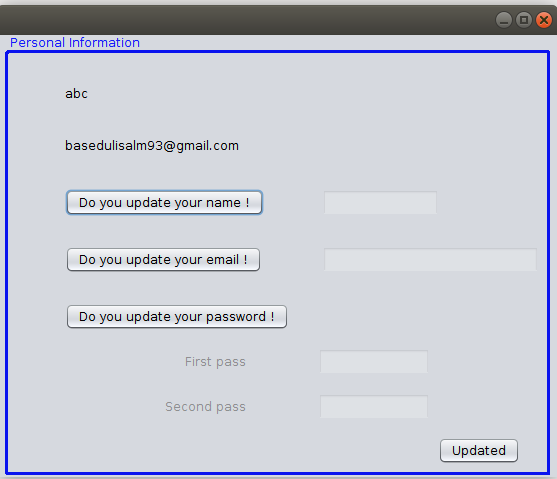
\includegraphics[height=5in]{/home/basedul/Documents/Report-writing-using-latex/ResturentManagementSystemReport/personalinfo.png}
		\caption{Design for Personal information update}
		\label{fig:personalinfo} 
\end{figure}
	\begin{lstlisting}
		/*
 * To change this license header, choose License Headers in Project Properties.
 * To change this template file, choose Tools | Templates
 * and open the template in the editor.
 */
package PersonalInfoShow;

import DatabaseConnection.DatabaseConnection;
import HomeActivity.MainActivity;
import RegistrationPackage.Admin.SignInClassForAdmin;
import java.awt.event.KeyEvent;
import java.sql.PreparedStatement;
import java.sql.ResultSet;
import java.sql.SQLException;
import java.util.logging.Level;
import java.util.logging.Logger;
import javax.swing.JFrame;
import javax.swing.JLabel;
import javax.swing.JOptionPane;

/**
 *
 * @author basedul
 */
public class PersonalInfoFrameForAdmin extends javax.swing.JFrame {

    /**
     * Creates new form PersonalInfoFrame
     */
    private String name = "";
    private String email = "";

    public PersonalInfoFrameForAdmin() {
        initComponents();
        setPersonalInfo();
    }

    public void setPersonalInfo() {
        PreparedStatement ps;
        ResultSet rs;
        String query = "SELECT * FROM `RegistrationForAdmin` WHERE `status` =?";
        try {
            ps = DatabaseConnection.getConnection().prepareStatement(query);
            ps.setInt(1, 1);
            rs = ps.executeQuery();
            if (rs.next()) {
                String name = rs.getString("u_u_name");
                this.name = name;
                showNameForAdminOnPersonalInfoFrame.setText(name);
                String email = rs.getString("U_mail");
                showEmailForAdminOnPersonalInfoFrame.setText(email);
            }
        } catch (SQLException ex) {
            Logger.getLogger(MainActivity.class.getName()).log(Level.SEVERE, null, ex);
        }
    }

    public JLabel getShowEmailOnPersonalInfoFrame() {
        return showEmailForAdminOnPersonalInfoFrame;
    }

    public JLabel getShowNameOnPersonalInfoFrame() {
        return showNameForAdminOnPersonalInfoFrame;
    }

    /**
     * This method is called from within the constructor to initialize the form.
     * WARNING: Do NOT modify this code. The content of this method is always
     * regenerated by the Form Editor.
     */
    @SuppressWarnings("unchecked")
    // <editor-fold defaultstate="collapsed" desc="Generated Code">                          
    private void initComponents() {

        jPanel1 = new javax.swing.JPanel();
        showNameForAdminOnPersonalInfoFrame = new javax.swing.JLabel();
        showEmailForAdminOnPersonalInfoFrame = new javax.swing.JLabel();
        updateNameButtonAdmin = new javax.swing.JButton();
        updateEmailButtonAdmin = new javax.swing.JButton();
        updatePassButtonAdmin = new javax.swing.JButton();
        updateNameAdmin = new javax.swing.JTextField();
        updateEmailAdmin = new javax.swing.JTextField();
        updateFirstPassAdmin = new javax.swing.JPasswordField();
        firstPassLabelAdmin = new javax.swing.JLabel();
        secondPassLabelAdmin = new javax.swing.JLabel();
        updateSecondPasswordAdmin = new javax.swing.JPasswordField();
        updatedButtonAdmin = new javax.swing.JButton();

        setDefaultCloseOperation(javax.swing.WindowConstants.EXIT_ON_CLOSE);

        jPanel1.setBorder(javax.swing.BorderFactory.createTitledBorder(new javax.swing.border.LineBorder(new java.awt.Color(10, 19, 238), 3, true), "Personal Information", javax.swing.border.TitledBorder.DEFAULT_JUSTIFICATION, javax.swing.border.TitledBorder.DEFAULT_POSITION, new java.awt.Font("Dialog", 0, 12), new java.awt.Color(16, 28, 253))); // NOI18N

        showNameForAdminOnPersonalInfoFrame.setText("Your name");

        showEmailForAdminOnPersonalInfoFrame.setText("Your email");

        updateNameButtonAdmin.setText("Do you update your name !");
        updateNameButtonAdmin.addMouseListener(new java.awt.event.MouseAdapter() {
            public void mouseClicked(java.awt.event.MouseEvent evt) {
                updateNameButtonAdminMouseClicked(evt);
            }
        });

        updateEmailButtonAdmin.setText("Do you update your email !");
        updateEmailButtonAdmin.addMouseListener(new java.awt.event.MouseAdapter() {
            public void mouseClicked(java.awt.event.MouseEvent evt) {
                updateEmailButtonAdminMouseClicked(evt);
            }
        });

        updatePassButtonAdmin.setText("Do you update your password !");
        updatePassButtonAdmin.addMouseListener(new java.awt.event.MouseAdapter() {
            public void mouseClicked(java.awt.event.MouseEvent evt) {
                updatePassButtonAdminMouseClicked(evt);
            }
        });

        updateNameAdmin.setEnabled(false);
        updateNameAdmin.addKeyListener(new java.awt.event.KeyAdapter() {
            public void keyPressed(java.awt.event.KeyEvent evt) {
                updateNameAdminKeyPressed(evt);
            }
        });

        updateEmailAdmin.setEnabled(false);
        updateEmailAdmin.addKeyListener(new java.awt.event.KeyAdapter() {
            public void keyPressed(java.awt.event.KeyEvent evt) {
                updateEmailAdminKeyPressed(evt);
            }
        });

        updateFirstPassAdmin.setEnabled(false);
        updateFirstPassAdmin.addKeyListener(new java.awt.event.KeyAdapter() {
            public void keyPressed(java.awt.event.KeyEvent evt) {
                updateFirstPassAdminKeyPressed(evt);
            }
        });

        firstPassLabelAdmin.setText("First pass");
        firstPassLabelAdmin.setEnabled(false);

        secondPassLabelAdmin.setText("Second pass");
        secondPassLabelAdmin.setEnabled(false);

        updateSecondPasswordAdmin.setEnabled(false);
        updateSecondPasswordAdmin.addKeyListener(new java.awt.event.KeyAdapter() {
            public void keyPressed(java.awt.event.KeyEvent evt) {
                updateSecondPasswordAdminKeyPressed(evt);
            }
        });

        updatedButtonAdmin.setText("Updated");
        updatedButtonAdmin.addMouseListener(new java.awt.event.MouseAdapter() {
            public void mouseClicked(java.awt.event.MouseEvent evt) {
                updatedButtonAdminMouseClicked(evt);
            }
        });

        javax.swing.GroupLayout jPanel1Layout = new javax.swing.GroupLayout(jPanel1);
        jPanel1.setLayout(jPanel1Layout);
        jPanel1Layout.setHorizontalGroup(
            jPanel1Layout.createParallelGroup(javax.swing.GroupLayout.Alignment.LEADING)
            .addGroup(jPanel1Layout.createSequentialGroup()
                .addGap(55, 55, 55)
                .addGroup(jPanel1Layout.createParallelGroup(javax.swing.GroupLayout.Alignment.LEADING)
                    .addGroup(jPanel1Layout.createSequentialGroup()
                        .addGroup(jPanel1Layout.createParallelGroup(javax.swing.GroupLayout.Alignment.LEADING)
                            .addComponent(showNameForAdminOnPersonalInfoFrame, javax.swing.GroupLayout.PREFERRED_SIZE, 240, javax.swing.GroupLayout.PREFERRED_SIZE)
                            .addComponent(showEmailForAdminOnPersonalInfoFrame, javax.swing.GroupLayout.PREFERRED_SIZE, 240, javax.swing.GroupLayout.PREFERRED_SIZE)
                            .addGroup(jPanel1Layout.createSequentialGroup()
                                .addGroup(jPanel1Layout.createParallelGroup(javax.swing.GroupLayout.Alignment.LEADING)
                                    .addGroup(jPanel1Layout.createSequentialGroup()
                                        .addComponent(updatePassButtonAdmin)
                                        .addGap(29, 29, 29))
                                    .addGroup(javax.swing.GroupLayout.Alignment.TRAILING, jPanel1Layout.createSequentialGroup()
                                        .addGroup(jPanel1Layout.createParallelGroup(javax.swing.GroupLayout.Alignment.TRAILING)
                                            .addComponent(firstPassLabelAdmin)
                                            .addComponent(secondPassLabelAdmin))
                                        .addGap(72, 72, 72)))
                                .addGroup(jPanel1Layout.createParallelGroup(javax.swing.GroupLayout.Alignment.LEADING, false)
                                    .addComponent(updateSecondPasswordAdmin, javax.swing.GroupLayout.DEFAULT_SIZE, 112, Short.MAX_VALUE)
                                    .addComponent(updateFirstPassAdmin)))
                            .addGroup(jPanel1Layout.createSequentialGroup()
                                .addComponent(updateNameButtonAdmin)
                                .addGap(58, 58, 58)
                                .addComponent(updateNameAdmin, javax.swing.GroupLayout.PREFERRED_SIZE, 117, javax.swing.GroupLayout.PREFERRED_SIZE)))
                        .addGap(0, 100, Short.MAX_VALUE))
                    .addGroup(jPanel1Layout.createSequentialGroup()
                        .addComponent(updateEmailButtonAdmin)
                        .addGap(60, 60, 60)
                        .addComponent(updateEmailAdmin)))
                .addContainerGap())
            .addGroup(javax.swing.GroupLayout.Alignment.TRAILING, jPanel1Layout.createSequentialGroup()
                .addContainerGap(javax.swing.GroupLayout.DEFAULT_SIZE, Short.MAX_VALUE)
                .addComponent(updatedButtonAdmin)
                .addGap(25, 25, 25))
        );
        jPanel1Layout.setVerticalGroup(
            jPanel1Layout.createParallelGroup(javax.swing.GroupLayout.Alignment.LEADING)
            .addGroup(jPanel1Layout.createSequentialGroup()
                .addGap(24, 24, 24)
                .addComponent(showNameForAdminOnPersonalInfoFrame, javax.swing.GroupLayout.PREFERRED_SIZE, 28, javax.swing.GroupLayout.PREFERRED_SIZE)
                .addGap(24, 24, 24)
                .addComponent(showEmailForAdminOnPersonalInfoFrame, javax.swing.GroupLayout.PREFERRED_SIZE, 28, javax.swing.GroupLayout.PREFERRED_SIZE)
                .addGap(30, 30, 30)
                .addGroup(jPanel1Layout.createParallelGroup(javax.swing.GroupLayout.Alignment.BASELINE)
                    .addComponent(updateNameButtonAdmin)
                    .addComponent(updateNameAdmin, javax.swing.GroupLayout.PREFERRED_SIZE, javax.swing.GroupLayout.DEFAULT_SIZE, javax.swing.GroupLayout.PREFERRED_SIZE))
                .addGap(30, 30, 30)
                .addGroup(jPanel1Layout.createParallelGroup(javax.swing.GroupLayout.Alignment.LEADING)
                    .addComponent(updateEmailButtonAdmin)
                    .addComponent(updateEmailAdmin, javax.swing.GroupLayout.PREFERRED_SIZE, javax.swing.GroupLayout.DEFAULT_SIZE, javax.swing.GroupLayout.PREFERRED_SIZE))
                .addGap(30, 30, 30)
                .addComponent(updatePassButtonAdmin)
                .addGap(18, 18, 18)
                .addGroup(jPanel1Layout.createParallelGroup(javax.swing.GroupLayout.Alignment.BASELINE)
                    .addComponent(updateFirstPassAdmin, javax.swing.GroupLayout.PREFERRED_SIZE, javax.swing.GroupLayout.DEFAULT_SIZE, javax.swing.GroupLayout.PREFERRED_SIZE)
                    .addComponent(firstPassLabelAdmin))
                .addGap(18, 18, 18)
                .addGroup(jPanel1Layout.createParallelGroup(javax.swing.GroupLayout.Alignment.BASELINE)
                    .addComponent(updateSecondPasswordAdmin, javax.swing.GroupLayout.PREFERRED_SIZE, javax.swing.GroupLayout.DEFAULT_SIZE, javax.swing.GroupLayout.PREFERRED_SIZE)
                    .addComponent(secondPassLabelAdmin))
                .addPreferredGap(javax.swing.LayoutStyle.ComponentPlacement.RELATED, 17, Short.MAX_VALUE)
                .addComponent(updatedButtonAdmin)
                .addContainerGap())
        );

        javax.swing.GroupLayout layout = new javax.swing.GroupLayout(getContentPane());
        getContentPane().setLayout(layout);
        layout.setHorizontalGroup(
            layout.createParallelGroup(javax.swing.GroupLayout.Alignment.LEADING)
            .addGroup(javax.swing.GroupLayout.Alignment.TRAILING, layout.createSequentialGroup()
                .addContainerGap()
                .addComponent(jPanel1, javax.swing.GroupLayout.DEFAULT_SIZE, javax.swing.GroupLayout.DEFAULT_SIZE, Short.MAX_VALUE)
                .addContainerGap())
        );
        layout.setVerticalGroup(
            layout.createParallelGroup(javax.swing.GroupLayout.Alignment.LEADING)
            .addComponent(jPanel1, javax.swing.GroupLayout.DEFAULT_SIZE, javax.swing.GroupLayout.DEFAULT_SIZE, Short.MAX_VALUE)
        );

        pack();
    }// </editor-fold>                        

    private void updatedButtonAdminMouseClicked(java.awt.event.MouseEvent evt) {                                                
        MainActivity mainActivity = new MainActivity();
        mainActivity.setVisible(true);
        mainActivity.setLocationRelativeTo(null);
        mainActivity.setDefaultCloseOperation(JFrame.EXIT_ON_CLOSE);
        this.dispose();
    }                                               

    private void updateNameButtonAdminMouseClicked(java.awt.event.MouseEvent evt) {                                                   
        updateNameAdmin.setEnabled(true);
        updateNameAdmin.requestFocus();
    }                                                  

    private void updateEmailButtonAdminMouseClicked(java.awt.event.MouseEvent evt) {                                                    
        updateEmailAdmin.setEnabled(true);
        updateEmailAdmin.requestFocus();
    }                                                   

    private void updatePassButtonAdminMouseClicked(java.awt.event.MouseEvent evt) {                                                   
        updateFirstPassAdmin.setEnabled(true);
        updateFirstPassAdmin.requestFocus();
        firstPassLabelAdmin.setEnabled(true);
        updateSecondPasswordAdmin.setEnabled(true);
        secondPassLabelAdmin.setEnabled(true);
    }                                                  

    private void updateNameAdminKeyPressed(java.awt.event.KeyEvent evt) {                                           
        if (evt.getKeyCode() == KeyEvent.VK_ENTER) {
            String name1 = updateNameAdmin.getText().toString();
            if (!name1.equals("")) {
                String query = "UPDATE `RegistrationForAdmin` SET `u_u_name`= ? WHERE `u_u_name`= ?";
                updateUserInfor(query, name1);
                updateNameAdmin.setText("");
                showNameForAdminOnPersonalInfoFrame.setText(name1);
                JOptionPane.showMessageDialog(null, "Successfully updated ");
                updateNameAdmin.setEnabled(false);
            }
        }
    }                                          

    private void updateEmailAdminKeyPressed(java.awt.event.KeyEvent evt) {                                            
        if (evt.getKeyCode() == KeyEvent.VK_ENTER) {
            String name1 = updateEmailAdmin.getText().toString();
            if (!name1.equals("")) {
                String query = "UPDATE `RegistrationForAdmin` SET `U_mail`= ? WHERE `u_u_name`= ?";
                updateUserInfor(query, name1);
                updateEmailAdmin.setText("");
                showEmailForAdminOnPersonalInfoFrame.setText(name1);
                JOptionPane.showMessageDialog(null, "Successfully updated ");
                updateEmailAdmin.setEnabled(false);
            }
        }
    }                                           

    private void updateFirstPassAdminKeyPressed(java.awt.event.KeyEvent evt) {                                                
        
    }                                               

    private void updateSecondPasswordAdminKeyPressed(java.awt.event.KeyEvent evt) {                                                     
        if (evt.getKeyCode() == KeyEvent.VK_ENTER) {
            String name1 = String.valueOf(updateFirstPassAdmin.getPassword());
            if (!name1.equals("")) {
                String pass2 = String.valueOf(updateSecondPasswordAdmin.getPassword());
                if(pass2.equals(name1)){
                    String query = "UPDATE `RegistrationForAdmin` SET `u_f_pass`= ? WHERE `u_u_name`= ?";
                    updateUserInfor(query, name1);
                    String query1 = "UPDATE `RegistrationForAdmin` SET `u_r_pass`= ? WHERE `u_u_name`= ?";
                    updateUserInfor(query1, pass2);
                    
                    
                    JOptionPane.showMessageDialog(null, "Successfully updated ");
                    updateFirstPassAdmin.setEnabled(false);
                    updateFirstPassAdmin.setText("");
                    firstPassLabelAdmin.setEnabled(false);
                    updateSecondPasswordAdmin.setEnabled(false);
                    updateSecondPasswordAdmin.setText("");
                    secondPassLabelAdmin.setEnabled(false);
                }else{
                    JOptionPane.showMessageDialog(null, "Password doesn't match");
                    updateSecondPasswordAdmin.requestFocus();
                }
                
            }else{
            }
        }
    }                                                    
    
    public void updateUserInfor(String query, String info){
        PreparedStatement psForStatusUpdate;
        //ResultSet resultSetForStatusUpdate;
        try {
            psForStatusUpdate = DatabaseConnection.getConnection().prepareStatement(query);
            psForStatusUpdate.setString(1, info);
            psForStatusUpdate.setString(2, name);
            psForStatusUpdate.executeUpdate();
        } catch (SQLException ex) {
            Logger.getLogger(SignInClassForAdmin.class.getName()).log(Level.SEVERE, null, ex);
        }
    }

    /**
     * @param args the command line arguments
     */
    public static void main(String args[]) {
        /* Set the Nimbus look and feel */
        //<editor-fold defaultstate="collapsed" desc=" Look and feel setting code (optional) ">
        /* If Nimbus (introduced in Java SE 6) is not available, stay with the default look and feel.
         * For details see http://download.oracle.com/javase/tutorial/uiswing/lookandfeel/plaf.html 
         */
        try {
            for (javax.swing.UIManager.LookAndFeelInfo info : javax.swing.UIManager.getInstalledLookAndFeels()) {
                if ("Nimbus".equals(info.getName())) {
                    javax.swing.UIManager.setLookAndFeel(info.getClassName());
                    break;
                }
            }
        } catch (ClassNotFoundException ex) {
            java.util.logging.Logger.getLogger(PersonalInfoFrameForAdmin.class.getName()).log(java.util.logging.Level.SEVERE, null, ex);
        } catch (InstantiationException ex) {
            java.util.logging.Logger.getLogger(PersonalInfoFrameForAdmin.class.getName()).log(java.util.logging.Level.SEVERE, null, ex);
        } catch (IllegalAccessException ex) {
            java.util.logging.Logger.getLogger(PersonalInfoFrameForAdmin.class.getName()).log(java.util.logging.Level.SEVERE, null, ex);
        } catch (javax.swing.UnsupportedLookAndFeelException ex) {
            java.util.logging.Logger.getLogger(PersonalInfoFrameForAdmin.class.getName()).log(java.util.logging.Level.SEVERE, null, ex);
        }
        //</editor-fold>
        //</editor-fold>

        /* Create and display the form */
        java.awt.EventQueue.invokeLater(new Runnable() {
            public void run() {
                new PersonalInfoFrameForAdmin().setVisible(true);
            }
        });
    }

    // Variables declaration - do not modify                     
    private javax.swing.JLabel firstPassLabelAdmin;
    private javax.swing.JPanel jPanel1;
    private javax.swing.JLabel secondPassLabelAdmin;
    private javax.swing.JLabel showEmailForAdminOnPersonalInfoFrame;
    private javax.swing.JLabel showNameForAdminOnPersonalInfoFrame;
    private javax.swing.JTextField updateEmailAdmin;
    private javax.swing.JButton updateEmailButtonAdmin;
    private javax.swing.JPasswordField updateFirstPassAdmin;
    private javax.swing.JTextField updateNameAdmin;
    private javax.swing.JButton updateNameButtonAdmin;
    private javax.swing.JButton updatePassButtonAdmin;
    private javax.swing.JPasswordField updateSecondPasswordAdmin;
    private javax.swing.JButton updatedButtonAdmin;
    // End of variables declaration                   
}

	\end{lstlisting}
	\subsubsection{Database Connection}
	\begin{lstlisting}
		
package DatabaseConnection;

import com.mysql.jdbc.Connection;
import java.sql.DriverManager;
import java.sql.SQLException;
import java.util.logging.Level;
import java.util.logging.Logger;

public class DatabaseConnection {
    // Database root and pass
    private static final String UserName = "root";// user name of database
    private static final String Password = "";// password of database
    private static final String ConnectionString = "jdbc:mysql://localhost/ResturentManagement";// connection with database
    
    // for database connection
    public static Connection getConnection() throws SQLException{
        Connection conn = null;// connection instances
        try {
            Class.forName("com.mysql.jdbc.Driver");
            conn = (Connection) DriverManager.getConnection(ConnectionString, UserName, Password);
        } catch (ClassNotFoundException ex) {
            Logger.getLogger(DatabaseConnection.class.getName()).log(Level.SEVERE, null, ex);
        }
        
        return conn;
    }
}

	\end{lstlisting}
	
	\subsubsection{Sign UP}
		\begin{figure}[H]
		\centering
		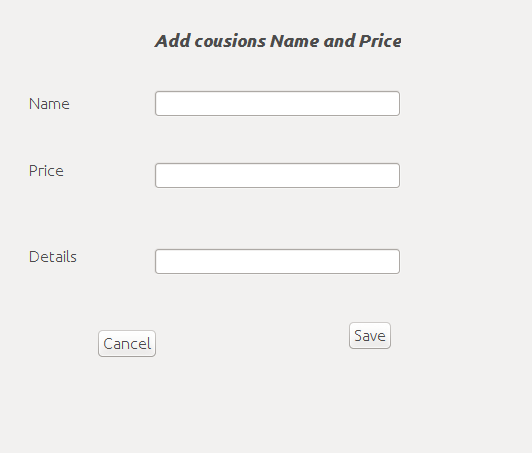
\includegraphics[height=5in]{/home/basedul/Documents/Report-writing-using-latex/ResturentManagementSystemReport/add.png}
		\caption{Design for Add new foods}
		\label{fig:addfoods} 
\end{figure}
	\begin{lstlisting}
		/*
 * To change this license header, choose License Headers in Project Properties.
 * To change this template file, choose Tools | Templates
 * and open the template in the editor.
 */
package FoodAddOnDatabase;

import DatabaseConnection.DatabaseConnection;
import HomeActivity.MainActivity;
import RegistrationPackage.SignUpClass;
import java.sql.PreparedStatement;
import java.sql.SQLException;
import java.util.logging.Level;
import java.util.logging.Logger;
import javax.swing.JFrame;
import javax.swing.JOptionPane;

public class Appetizers extends javax.swing.JFrame {

    /**
     * Creates new form AddMeal
     */
    public Appetizers() {
        initComponents();
        setLocationRelativeTo(null);
        setResizable(false);
    }

    /**
     * This method is called from within the constructor to initialize the form.
     * WARNING: Do NOT modify this code. The content of this method is always
     * regenerated by the Form Editor.
     */
    @SuppressWarnings("unchecked")
    // <editor-fold defaultstate="collapsed" desc="Generated Code">                          
    private void initComponents() {

        jLabel1 = new javax.swing.JLabel();
        jLabel2 = new javax.swing.JLabel();
        jLabel3 = new javax.swing.JLabel();
        meal_name_in_add_class = new javax.swing.JTextField();
        price_name_in_add_class = new javax.swing.JTextField();
        save_button_for_add_class = new javax.swing.JButton();
        cancell_button_for_add_class = new javax.swing.JButton();
        jLabel4 = new javax.swing.JLabel();
        Details_name_in_add_class = new javax.swing.JTextField();

        setDefaultCloseOperation(javax.swing.WindowConstants.EXIT_ON_CLOSE);

        jLabel1.setFont(new java.awt.Font("Ubuntu", 3, 18)); // NOI18N
        jLabel1.setText("Add cousions Name and Price");

        jLabel2.setText("Name");

        jLabel3.setText("Price");

        meal_name_in_add_class.setToolTipText("Enter name of meal");

        price_name_in_add_class.setToolTipText("Enter price of meal");

        save_button_for_add_class.setText("Save");
        save_button_for_add_class.addMouseListener(new java.awt.event.MouseAdapter() {
            public void mouseClicked(java.awt.event.MouseEvent evt) {
                save_button_for_add_classMouseClicked(evt);
            }
        });

        cancell_button_for_add_class.setText("Cancel");
        cancell_button_for_add_class.addMouseListener(new java.awt.event.MouseAdapter() {
            public void mouseClicked(java.awt.event.MouseEvent evt) {
                cancell_button_for_add_classMouseClicked(evt);
            }
        });

        jLabel4.setText("Details");

        Details_name_in_add_class.setToolTipText("Enter price of meal");

        javax.swing.GroupLayout layout = new javax.swing.GroupLayout(getContentPane());
        getContentPane().setLayout(layout);
        layout.setHorizontalGroup(
            layout.createParallelGroup(javax.swing.GroupLayout.Alignment.LEADING)
            .addGroup(layout.createSequentialGroup()
                .addGroup(layout.createParallelGroup(javax.swing.GroupLayout.Alignment.TRAILING, false)
                    .addGroup(layout.createSequentialGroup()
                        .addGap(30, 30, 30)
                        .addGroup(layout.createParallelGroup(javax.swing.GroupLayout.Alignment.LEADING)
                            .addComponent(jLabel2)
                            .addComponent(jLabel3)
                            .addComponent(jLabel4))
                        .addGap(77, 77, 77)
                        .addGroup(layout.createParallelGroup(javax.swing.GroupLayout.Alignment.LEADING, false)
                            .addComponent(jLabel1, javax.swing.GroupLayout.DEFAULT_SIZE, javax.swing.GroupLayout.DEFAULT_SIZE, Short.MAX_VALUE)
                            .addComponent(meal_name_in_add_class)
                            .addComponent(price_name_in_add_class)
                            .addComponent(Details_name_in_add_class)))
                    .addGroup(javax.swing.GroupLayout.Alignment.LEADING, layout.createSequentialGroup()
                        .addGap(98, 98, 98)
                        .addComponent(cancell_button_for_add_class)
                        .addPreferredGap(javax.swing.LayoutStyle.ComponentPlacement.RELATED, javax.swing.GroupLayout.DEFAULT_SIZE, Short.MAX_VALUE)
                        .addComponent(save_button_for_add_class)
                        .addGap(9, 9, 9)))
                .addContainerGap(132, Short.MAX_VALUE))
        );
        layout.setVerticalGroup(
            layout.createParallelGroup(javax.swing.GroupLayout.Alignment.LEADING)
            .addGroup(layout.createSequentialGroup()
                .addGap(30, 30, 30)
                .addComponent(jLabel1)
                .addGap(39, 39, 39)
                .addGroup(layout.createParallelGroup(javax.swing.GroupLayout.Alignment.BASELINE)
                    .addComponent(jLabel2)
                    .addComponent(meal_name_in_add_class, javax.swing.GroupLayout.PREFERRED_SIZE, javax.swing.GroupLayout.DEFAULT_SIZE, javax.swing.GroupLayout.PREFERRED_SIZE))
                .addGap(45, 45, 45)
                .addGroup(layout.createParallelGroup(javax.swing.GroupLayout.Alignment.LEADING)
                    .addComponent(jLabel3)
                    .addComponent(price_name_in_add_class, javax.swing.GroupLayout.PREFERRED_SIZE, javax.swing.GroupLayout.DEFAULT_SIZE, javax.swing.GroupLayout.PREFERRED_SIZE))
                .addGap(59, 59, 59)
                .addGroup(layout.createParallelGroup(javax.swing.GroupLayout.Alignment.LEADING)
                    .addComponent(Details_name_in_add_class, javax.swing.GroupLayout.PREFERRED_SIZE, javax.swing.GroupLayout.DEFAULT_SIZE, javax.swing.GroupLayout.PREFERRED_SIZE)
                    .addComponent(jLabel4))
                .addGroup(layout.createParallelGroup(javax.swing.GroupLayout.Alignment.LEADING)
                    .addGroup(layout.createSequentialGroup()
                        .addGap(54, 54, 54)
                        .addComponent(cancell_button_for_add_class))
                    .addGroup(layout.createSequentialGroup()
                        .addGap(46, 46, 46)
                        .addComponent(save_button_for_add_class)))
                .addGap(248, 248, 248))
        );

        pack();
    }// </editor-fold>                        

    private void cancell_button_for_add_classMouseClicked(java.awt.event.MouseEvent evt) {                                                          
        MainActivity homepage = new MainActivity();
        homepage.setVisible(true);
        homepage.setLocationRelativeTo(null);
        homepage.setDefaultCloseOperation(JFrame.EXIT_ON_CLOSE);
        dispose();
    }                                                         

    private void save_button_for_add_classMouseClicked(java.awt.event.MouseEvent evt) {                                                       
        String mName = meal_name_in_add_class.getText().toString().trim();
        //float mPrice = Float.valueOf(price_name_in_add_class.getText().toString());
        if (!mName.equals("")) {
            String mPrice = price_name_in_add_class.getText().toString();
            if (!mPrice.equals("")) {
                String apDetails = Details_name_in_add_class.getText().toString();
                if (!apDetails.equals("")) {
                    try {
                        float m_price = (float) Integer.parseInt(mPrice);

                        PreparedStatement ps;
                        String query = "INSERT INTO `APPETIZERS`(`app_name`, `app_price`, `details_of_App`) VALUES (?,?,?)";

                        try {

                            ps = DatabaseConnection.getConnection().prepareStatement(query);

                            ps.setString(1, mName);
                            ps.setFloat(2, m_price);
                            ps.setString(3, apDetails);

                            if (ps.executeUpdate() > 0) {
                                JOptionPane.showMessageDialog(null, "New value Add");
                                MainActivity homepage = new MainActivity();
                                homepage.setVisible(true);
                                homepage.setLocationRelativeTo(null);
                                homepage.setDefaultCloseOperation(JFrame.EXIT_ON_CLOSE);
                                dispose();
                            }

                        } catch (SQLException ex) {
                            Logger.getLogger(SignUpClass.class.getName()).log(Level.SEVERE, null, ex);
                        }
                    } catch (NumberFormatException en) {
                        JOptionPane.showMessageDialog(rootPane, "Enter Float value");
                        price_name_in_add_class.setText("");
                        price_name_in_add_class.requestFocus();
                    }
                }else{
                    Details_name_in_add_class.setText("");
                    Details_name_in_add_class.requestFocus();
                }

            } else {
                JOptionPane.showMessageDialog(rootPane, "Enter correct value");
                price_name_in_add_class.setText("");
                price_name_in_add_class.requestFocus();
            }
        } else {
            JOptionPane.showMessageDialog(rootPane, "Enter correct name");
            meal_name_in_add_class.setText("");
            meal_name_in_add_class.requestFocus();
        }

    }                                                      

    /**
     * @param args the command line arguments
     */
    public static void main(String args[]) {
        /* Set the Nimbus look and feel */
        //<editor-fold defaultstate="collapsed" desc=" Look and feel setting code (optional) ">
        /* If Nimbus (introduced in Java SE 6) is not available, stay with the default look and feel.
         * For details see http://download.oracle.com/javase/tutorial/uiswing/lookandfeel/plaf.html 
         */
        try {
            for (javax.swing.UIManager.LookAndFeelInfo info : javax.swing.UIManager.getInstalledLookAndFeels()) {
                if ("Nimbus".equals(info.getName())) {
                    javax.swing.UIManager.setLookAndFeel(info.getClassName());
                    break;
                }
            }
        } catch (ClassNotFoundException ex) {
            java.util.logging.Logger.getLogger(Appetizers.class.getName()).log(java.util.logging.Level.SEVERE, null, ex);
        } catch (InstantiationException ex) {
            java.util.logging.Logger.getLogger(Appetizers.class.getName()).log(java.util.logging.Level.SEVERE, null, ex);
        } catch (IllegalAccessException ex) {
            java.util.logging.Logger.getLogger(Appetizers.class.getName()).log(java.util.logging.Level.SEVERE, null, ex);
        } catch (javax.swing.UnsupportedLookAndFeelException ex) {
            java.util.logging.Logger.getLogger(Appetizers.class.getName()).log(java.util.logging.Level.SEVERE, null, ex);
        }
        //</editor-fold>
        //</editor-fold>
        //</editor-fold>
        //</editor-fold>

        /* Create and display the form */
        java.awt.EventQueue.invokeLater(new Runnable() {
            public void run() {
                new Appetizers().setVisible(true);
            }
        });
    }

    // Variables declaration - do not modify                     
    private javax.swing.JTextField Details_name_in_add_class;
    private javax.swing.JButton cancell_button_for_add_class;
    private javax.swing.JLabel jLabel1;
    private javax.swing.JLabel jLabel2;
    private javax.swing.JLabel jLabel3;
    private javax.swing.JLabel jLabel4;
    private javax.swing.JTextField meal_name_in_add_class;
    private javax.swing.JTextField price_name_in_add_class;
    private javax.swing.JButton save_button_for_add_class;
    // End of variables declaration                   
}

	\end{lstlisting}
	{\bfseries \Large Database Query}
	\begin{lstlisting}[
           language=SQL,
           showspaces=false,
           basicstyle=\ttfamily,
           numbers=left,
           numberstyle=\tiny,
           commentstyle=\color{gray}
        ]
		1. Create database ResturentManagement;
		
		2. CREATE TABLE RegistrationForAdmin (
		u_id TINYINT UNSIGNED NOT NULL AUTO_INCREMENT,
		u_f_name varchar(80),
		u_l_name varchar(80),
		u_u_name varchar(80),
		U_mail varchar(50),
		u_f_pass varchar(20),
		u_r_pass varchar(20),
		status int(11)
		PRIMARY KEY (u_id)
		)ENGINE=InnoDB DEFAULT CHARSET=utf8;
		
		3. CREATE TABLE Salad (
		sl_id TINYINT UNSIGNED NOT NULL AUTO_INCREMENT,
		sl_name varchar(255),
		sl_price float(10, 2),
		sl_details varchar(255),
		PRIMARY KEY (sl_id)
		)ENGINE=InnoDB DEFAULT CHARSET=utf8;

 		4. CREATE TABLE Soups (
		so_id TINYINT UNSIGNED NOT NULL AUTO_INCREMENT,
		so_name varchar(255),
		so_price float(10, 2),
		so_details varchar(255),
		PRIMARY KEY (so_id)
		)ENGINE=InnoDB DEFAULT CHARSET=utf8;

  		5. CREATE TABLE Chicken (
		ck_id TINYINT UNSIGNED NOT NULL AUTO_INCREMENT,
		ck_name varchar(255),
		ck_price float(10, 2),
		ck_details varchar(255),
		PRIMARY KEY (ck_id)
		)ENGINE=InnoDB DEFAULT CHARSET=utf8;

		6. CREATE TABLE Pork (
		po_id TINYINT UNSIGNED NOT NULL AUTO_INCREMENT,
		po_name varchar(255),
		po_price float(10, 2),
		po_details varchar(255),
		PRIMARY KEY (po_id)
		)ENGINE=InnoDB DEFAULT CHARSET=utf8;

	 	7. CREATE TABLE BeefLamb (
		bl_id TINYINT UNSIGNED NOT NULL AUTO_INCREMENT,
		bl_name varchar(255),
		bl_price float(10, 2),
		bl_details varchar(255),
		PRIMARY KEY (bl_id)
		)ENGINE=InnoDB DEFAULT CHARSET=utf8;

		8. CREATE TABLE SeaFood (
		sf_id TINYINT UNSIGNED NOT NULL AUTO_INCREMENT,
		sf_name varchar(255),
		sf_price float(10, 2),
		sf_details varchar(255),
		PRIMARY KEY (sf_id)
		)ENGINE=InnoDB DEFAULT CHARSET=utf8;

	 	9. CREATE TABLE NoddlesRice (
		nr_id TINYINT UNSIGNED NOT NULL AUTO_INCREMENT,
		nr_name varchar(255),
		nr_price float(10, 2),
		nr_details varchar(255),
		PRIMARY KEY (nr_id)
		)ENGINE=InnoDB DEFAULT CHARSET=utf8;

	 	10. CREATE TABLE VegeTofu (
		vt_id TINYINT UNSIGNED NOT NULL AUTO_INCREMENT,
		vt_name varchar(255),
		vt_price float(10, 2),
		vt_details varchar(255),
		PRIMARY KEY (vt_id)
		)ENGINE=InnoDB DEFAULT CHARSET=utf8;

	 	11. CREATE TABLE ClientOrderList (
		col_id TINYINT UNSIGNED NOT NULL AUTO_INCREMENT,
		col_name varchar(255),
		col_price float(10, 2),
		UserName varchar(255),
		PRIMARY KEY (col_id)
		)ENGINE=InnoDB DEFAULT CHARSET=utf8;

	 	12. ALTER TABLE `ClientOrderList` ADD `UserName` VARCHAR(255) NOT NULL AFTER `col_price`;

	 	13. CREATE TABLE RankList (
		rl_id TINYINT UNSIGNED NOT NULL AUTO_INCREMENT,
		rl_name varchar(255),
		rl_score int,
		rl_comments varchar(255),
		PRIMARY KEY (rl_id)
		)ENGINE=InnoDB DEFAULT CHARSET=utf8;
		
	 	14. ALTER TABLE `Registration` ADD `reward_point` float(10, 2) NOT NULL AFTER `status`;
		
\end{lstlisting}
	\end{comment}
	
	\subsection{Test Case}
		\begin{table}[H]
		\label{tab:Test}
\caption{Test Cases}
\vspace{0.2cm}
\begin{tabular}{|M{2.5cm}|M{4cm}|M{4cm}|M{4cm}|M{4cm}|M{4cm}|M{4cm}|M{1cm}|N}
%Start
\hline
\textbf{Scenario} &
\multicolumn{2}{M{3.5cm}|}{\textbf{Test Cases}} & 
\multicolumn{2}{M{3.5cm}|}{\textbf{Expected Result}} & %
\multicolumn{2}{M{3.5cm}|}{\textbf{Test Result}} &
\textbf{Pass or Fail} & \\ [25pt]
\hline
\hline%Start
\multirow{3}{1.5cm}[-1.5em]{\centering Registration} &

\multicolumn{2}{M{3.5cm}|}{\begin{flushleft}
Enter null in
mandatory fields.
\end{flushleft}} &
\multicolumn{2}{M{3.5cm}|}{\begin{flushleft}
It should not do the
registration
and show error.
\end{flushleft}} & %
\multicolumn{2}{M{3.5cm}|}{\begin{flushleft}
It will show message
that please fill out this
field.
\end{flushleft}} &
Pass & \\[15pt]\cline{2-9} &
\multicolumn{2}{M{3.5cm}|}{\begin{flushleft}
Enter incorrect data
\end{flushleft}} & 
\multicolumn{2}{M{3.5cm}|}{\begin{flushleft}
It should not do the
registration and show error.
\end{flushleft}} & 
\multicolumn{2}{M{3.5cm}|}{\begin{flushleft}
Email: Please enter an email.
\linebreak
Password: Password.\linebreak
do not match\end{flushleft}} & Pass\\[25pt]\cline{2-9}& 
\multicolumn{2}{M{3.5cm}|}{\begin{flushleft}
Enter correct data of all 
required field
\end{flushleft}} & 
\multicolumn{2}{M{3.5cm}|}{\begin{flushleft}
It should lead to successfully registration
\end{flushleft}} & 
\multicolumn{2}{M{3.5cm}|}{\begin{flushleft}
It will show the message of successfully registrattion
\end{flushleft}} & Pass\\ [25pt]
\hline
%End
\hline%Start
\multirow{3}{1.5cm}[-1.5em]{\centering Login} &

\multicolumn{2}{M{3.5cm}|}{\begin{flushleft}
Enter null email or
password.
\end{flushleft}} &
\multicolumn{2}{M{3.5cm}|}{\begin{flushleft}
It should not do the
login and show error.
\end{flushleft}
} & %
\multicolumn{2}{M{3.5cm}|}{\begin{flushleft}
It will show message that please fill out this field.
\end{flushleft}} &
Pass & \\[15pt]\cline{2-9} &
\multicolumn{2}{M{3.5cm}|}{\begin{flushleft}
Enter wrong data of
email or password.
\end{flushleft}} & 
\multicolumn{2}{M{3.5cm}|}{\begin{flushleft}
It should not do the login and show error.
\end{flushleft}} & 
\multicolumn{2}{M{3.5cm}|}{\begin{flushleft}
It will show message that please enter an email or your email address or password are not correct.
\end{flushleft}
} & Pass\\[25pt]\cline{2-9}& 
\multicolumn{2}{M{3.5cm}|}{\begin{flushleft}
Enter correct data of
email or password.
\end{flushleft}} & 
\multicolumn{2}{M{3.5cm}|}{\begin{flushleft}
It should let do the login.
\end{flushleft}
} & 
\multicolumn{2}{M{3.5cm}|}{\begin{flushleft}
It will redirect to your all purchased products
\end{flushleft}
} & Pass\\ [25pt]
\hline%End
%\hline%Start
%\multirow{3}{1.5cm}[-1.5em]{\centering Update password
%} &
%
%\multicolumn{2}{M{3.5cm}|}{\begin{flushleft}
%Enter null in
%mandatory fields.
%\end{flushleft}
%} &
%\multicolumn{2}{M{3.5cm}|}{\begin{flushleft}
%It should not do the update
%and show error.
%\end{flushleft}} & %
%\multicolumn{2}{M{3.5cm}|}{\begin{flushleft}
%It will show message that please fill out this field.
%\end{flushleft}} &
%Pass & \\[15pt]\cline{2-9} &
%\multicolumn{2}{M{3.5cm}|}{\begin{flushleft}
%Enter incorrect data
%\end{flushleft}} & 
%\multicolumn{2}{M{3.5cm}|}{\begin{flushleft}
%It should not do the update
%and show error.
%\end{flushleft}} & 
%\multicolumn{2}{M{3.5cm}|}{\begin{flushleft}
%It will show the message that the old password do not match.
%\end{flushleft}
%} & Pass\\[25pt]\cline{2-9}& 
%\multicolumn{2}{M{3.5cm}|}{\begin{flushleft}
%Enter correct data of all
%required field.
%\end{flushleft}} & 
%\multicolumn{2}{M{3.5cm}|}{\begin{flushleft}
%It should let do
%registration.
%\end{flushleft}} & 
%
%\multicolumn{2}{M{3.5cm}|}{\begin{flushleft}
%It will show the message that password successfully updated.
%\end{flushleft}
%} & Pass\\ [25pt]
%\hline%End
%\hline%Start
%\multirow{2}{1.5cm}[-1.5em]{\centering Search Food
%} &
%
%\multicolumn{2}{M{3.5cm}|}{\begin{flushleft}
%Enter null or incorrect data in search fields.
%\end{flushleft}
%} &
%\multicolumn{2}{M{3.5cm}|}{\begin{flushleft}
%It will not search food
%\end{flushleft}} & %
%\multicolumn{2}{M{3.5cm}|}{\begin{flushleft}
%It will show the message that there was no search results!
%\end{flushleft}} &
%Pass & \\[15pt]\cline{2-9} &
%\multicolumn{2}{M{3.5cm}|}{\begin{flushleft}
%Enter correct data in
%Search fields.
%\end{flushleft}} & 
%\multicolumn{2}{M{3.5cm}|}{\begin{flushleft}
%It should search foods depending the keywords.
%\end{flushleft}} & 
%\multicolumn{2}{M{3.5cm}|}{\begin{flushleft}
%It will display the foods regarding the keywords.
%\end{flushleft}
%} & Pass\\[25pt]
%\hline%End
%\hline%Start
%\multirow{2}{1.5cm}[-1.5em]{\centering Comment Food
%} &
%
%\multicolumn{2}{M{3.5cm}|}{\begin{flushleft}
%Enter non ASCII character.
%\end{flushleft}} &
%\multicolumn{2}{M{3.5cm}|}{\begin{flushleft}
%It will not let to comment
%\end{flushleft}
%} & %
%\multicolumn{2}{M{3.5cm}|}{\begin{flushleft}
%It will show error as unsupported character.
%\end{flushleft}} &
%Pass & \\[15pt]\cline{2-9} &
%\multicolumn{2}{M{3.5cm}|}{\begin{flushleft}
%Enter ASCII character.
%\end{flushleft}} & 
%\multicolumn{2}{M{3.5cm}|}{\begin{flushleft}
%It will lead a successful comment.
%\end{flushleft}} & 
%\multicolumn{2}{M{3.5cm}|}{\begin{flushleft}
%It will view the succession of a comment.
%\end{flushleft}
%} & Pass\\[25pt]
%\hline%End

\end{tabular}
\end{table}

\begin{table}[H]
\captionsetup{labelformat=empty}
\caption[]{ }
\vspace{0.2cm}
\begin{tabular}{|M{2.5cm}|M{4cm}|M{4cm}|M{4cm}|M{4cm}|M{4cm}|M{4cm}|M{1cm}|N}
%Start
\hline
\textbf{Scenario} &
\multicolumn{2}{M{3.5cm}|}{\textbf{Test Cases}} & 
\multicolumn{2}{M{3.5cm}|}{\textbf{Expected Result}} & %
\multicolumn{2}{M{3.5cm}|}{\textbf{Test Result}} &
\textbf{Pass or Fail} & \\ [25pt]
\hline
%\hline%Start
%\multirow{3}{1.5cm}[-1.5em]{\centering Registration} &
%
%\multicolumn{2}{M{3.5cm}|}{\begin{flushleft}
%Enter null in
%mandatory fields.
%\end{flushleft}} &
%\multicolumn{2}{M{3.5cm}|}{\begin{flushleft}
%It should not do the
%registration
%and show error.
%\end{flushleft}} & %
%\multicolumn{2}{M{3.5cm}|}{\begin{flushleft}
%It will show message
%that please fill out this
%field.
%\end{flushleft}} &
%Pass & \\[15pt]\cline{2-9} &
%\multicolumn{2}{M{3.5cm}|}{\begin{flushleft}
%Enter incorrect data
%\end{flushleft}} & 
%\multicolumn{2}{M{3.5cm}|}{\begin{flushleft}
%It should not do the
%registration and show error.
%\end{flushleft}} & 
%\multicolumn{2}{M{3.5cm}|}{\begin{flushleft}
%Email: Please enter an email.
%\linebreak
%Password: Password.\linebreak
%do not match\end{flushleft}} & Pass\\[25pt]\cline{2-9}& 
%\multicolumn{2}{M{3.5cm}|}{\begin{flushleft}
%Enter correct data of all 
%required field
%\end{flushleft}} & 
%\multicolumn{2}{M{3.5cm}|}{\begin{flushleft}
%It should lead to successfully registration
%\end{flushleft}} & 
%\multicolumn{2}{M{3.5cm}|}{\begin{flushleft}
%It will show the message of successfully registrattion
%\end{flushleft}} & Pass\\ [25pt]
%\hline
%%End
%\hline%Start
%\multirow{3}{1.5cm}[-1.5em]{\centering Login} &
%
%\multicolumn{2}{M{3.5cm}|}{\begin{flushleft}
%Enter null email or
%password.
%\end{flushleft}} &
%\multicolumn{2}{M{3.5cm}|}{\begin{flushleft}
%It should not do the
%login and show error.
%\end{flushleft}
%} & %
%\multicolumn{2}{M{3.5cm}|}{\begin{flushleft}
%It will show message that please fill out this field.
%\end{flushleft}} &
%Pass & \\[15pt]\cline{2-9} &
%\multicolumn{2}{M{3.5cm}|}{\begin{flushleft}
%Enter wrong data of
%email or password.
%\end{flushleft}} & 
%\multicolumn{2}{M{3.5cm}|}{\begin{flushleft}
%It should not do the login and show error.
%\end{flushleft}} & 
%\multicolumn{2}{M{3.5cm}|}{\begin{flushleft}
%It will show message that please enter an email or your email address or password are not correct.
%\end{flushleft}
%} & Pass\\[25pt]\cline{2-9}& 
%\multicolumn{2}{M{3.5cm}|}{\begin{flushleft}
%Enter correct data of
%email or password.
%\end{flushleft}} & 
%\multicolumn{2}{M{3.5cm}|}{\begin{flushleft}
%It should let do the login.
%\end{flushleft}
%} & 
%\multicolumn{2}{M{3.5cm}|}{\begin{flushleft}
%It will redirect to your all purchased products
%\end{flushleft}
%} & Pass\\ [25pt]
%\hline%End
\hline%Start
\multirow{3}{2cm}[-1.5em]{\centering Update password
} &

\multicolumn{2}{M{3.5cm}|}{\begin{flushleft}
Enter null in
mandatory fields.
\end{flushleft}
} &
\multicolumn{2}{M{3.5cm}|}{\begin{flushleft}
It should not do the update
and show error.
\end{flushleft}} & %
\multicolumn{2}{M{3.5cm}|}{\begin{flushleft}
It will show message that please fill out this field.
\end{flushleft}} &
Pass & \\[15pt]\cline{2-9} &
\multicolumn{2}{M{3.5cm}|}{\begin{flushleft}
Enter incorrect data
\end{flushleft}} & 
\multicolumn{2}{M{3.5cm}|}{\begin{flushleft}
It should not do the update
and show error.
\end{flushleft}} & 
\multicolumn{2}{M{3.5cm}|}{\begin{flushleft}
It will show the message that the old password do not match.
\end{flushleft}
} & Pass\\[25pt]\cline{2-9}& 
\multicolumn{2}{M{3.5cm}|}{\begin{flushleft}
Enter correct data of all
required field.
\end{flushleft}} & 
\multicolumn{2}{M{3.5cm}|}{\begin{flushleft}
It should let do
registration.
\end{flushleft}} & 

\multicolumn{2}{M{3.5cm}|}{\begin{flushleft}
It will show the message that password successfully updated.
\end{flushleft}
} & Pass\\ [25pt]
\hline%End
\hline%Start
\multirow{2}{1.5cm}[-1.5em]{\centering Search Food
} &

\multicolumn{2}{M{3.5cm}|}{\begin{flushleft}
Enter null or incorrect data in search fields.
\end{flushleft}
} &
\multicolumn{2}{M{3.5cm}|}{\begin{flushleft}
It will not search food
\end{flushleft}} & %
\multicolumn{2}{M{3.5cm}|}{\begin{flushleft}
It will show the message that there was no search results!
\end{flushleft}} &
Pass & \\[15pt]\cline{2-9} &
\multicolumn{2}{M{3.5cm}|}{\begin{flushleft}
Enter correct data in
Search fields.
\end{flushleft}} & 
\multicolumn{2}{M{3.5cm}|}{\begin{flushleft}
It should search foods depending the keywords.
\end{flushleft}} & 
\multicolumn{2}{M{3.5cm}|}{\begin{flushleft}
It will display the foods regarding the keywords.
\end{flushleft}
} & Pass\\[25pt]
\hline%End
\hline%Start
\multirow{2}{1.5cm}[-1.5em]{\centering Comment Food
} &

\multicolumn{2}{M{3.5cm}|}{\begin{flushleft}
Enter non ASCII character.
\end{flushleft}} &
\multicolumn{2}{M{3.5cm}|}{\begin{flushleft}
It will not let to comment
\end{flushleft}
} & %
\multicolumn{2}{M{3.5cm}|}{\begin{flushleft}
It will show error as unsupported character.
\end{flushleft}} &
Pass & \\[15pt]\cline{2-9} &
\multicolumn{2}{M{3.5cm}|}{\begin{flushleft}
Enter ASCII character.
\end{flushleft}} & 
\multicolumn{2}{M{3.5cm}|}{\begin{flushleft}
It will lead a successful comment.
\end{flushleft}} & 
\multicolumn{2}{M{3.5cm}|}{\begin{flushleft}
It will view the succession of a comment.
\end{flushleft}
} & Pass\\[25pt]
\hline%End

\end{tabular}
\end{table}
	\subsection{Code Documentation}
	\tab Code documentation is an important part of any software engineering project. Throughout the im-
plementation, a JavaDoc tool was used to generate HTML API documentation of the project. The
JavaDoc could then be used to provide assistance to any future developer.

	\subsection{Version Control}
	\tab Due to the type of development methodology used for this project, incremental backups of the system
were required. Version control systems (also known as Revision control) such as Mercurial manage
the changes to documents storing each backup in its own revision with the ability to restore back to a
particular version in the event of debugging.
	
		

	\subsection{Chapter Summary}
	\tab This chapter has discussed the interesting aspects from the implementation stage. The next chapter
documents the results by demonstrating the working system.
	
	\newpage	
	\section{Conclusion}
	%{\bfseries \Large Conclusion}
	\subsection{Chapter Overview}
		\tab This chapters draws the project report to a close and reflects on the design decisions made throughout.
It also discusses possible future development ideas.

	\subsection{Project Overview}
	\tab The system achieved all of its proposed priority 1 and priority 2 functional requirements and even some
priority 3 outlined in Section \ref{sec:prioty}.
However, the initial project plan and gannt chart had to be modified as the project became about
a month behind due to underestimations on the time to implement some desired features. This meant
that some of the lower priority requirements had to be scrapped.
	\subsection{Further Development}
	\tab This project was developed under time constraints of 120 hours. Therefore the proposed features
specified in the requirements were what the developer thought to be realistic targets.
However, if more time became available the following could be implemented.
%	\subsubsection{Graphical User Interface (GUI)}
%	\tab Currently the GUI was adequate to do the job but maybe the GUI could have had a more appealing
%look and feel. This all beckons on whether or not Java was the best programming language to use to
%generate the best looking GUI. Maybe a web developed GUI could have been a better alternative but
%with the developer having little experience in web development this would not have been ideal.
	\subsubsection{Table Management}
	\tab A feature that was thought of as a possibility but never documented past the design stage was the use
of a table management feature. This would give the system the ability to reserve and allocate tables.
The table data could then be used to help predict how busy the restaurant may be and help prepare
the staff rota.
	\subsection{Reflection}
	\tab On reflection, even though the majority of the proposed features were completed and the project was
deemed a huge success, the author felt that he could have been more disciplined in keeping to the plan.
He also felt that the proposed features were slightly unrealistic and some even unnecessary.
For the general project, the author felt that important aspects of research were not undertaken
including interviews with restaurant owners and user questionnaires. This would have provided good
insight into existing solutions.
	\subsection{Skills Attained}
	\tab This project has helped the author to attain new skills as well as develop existing skills. The skills
attained have been both technical and individual with the main individual skill being project manage-
ment which required good time keeping and management of the workload. \\
Some technical skills that
have been developed include:
	\begin{itemize}
		\item Advanced coding using the Java Swing interface.
		\item Relational database schema design and trigger coding.
		\item Advanced coding using Java threads.
	\end{itemize}
\subsection{Chapter Summary}	
\tab This chapter has concluded the project report and provided an insight into possible future development.
	


\newpage
\bibliography{/home/basedul/Documents/Report-writing-using-latex/ResturentManagementSystemReport/req.bib}
\bibliographystyle{IEEEtran}
\newpage
\section*{Acknowledgement}
\addcontentsline{toc}{section}{\textbf{Acknowledgement}}
	\tab Foremost, I would like to express my sincere gratitude to the almighty Allah for His blessings and protection throughout my undergraduate studies.\\ 
\tab My sincere thanks to my supervisor,  \textbf{Liang Zhao} for the continuous support of my Bachelor's study, patience, motivation, enthusiasm, and immense knowledge. His guidance helped me in all the time of research and writing of this thesis. I could not have imagined having a better advisor and mentor.\\
        \tab I also thank my fellow classmates, my friends and for all the fun we have had in the last four years.\\
        \tab Last but not the least; I would like to thank my parents \textbf{Mr. Syed Amin Uddin} and \textbf{Mrs. Hajera Amin} and \textbf{Ms. Noorjahan Khanam} for their prayers, support, encouragement and their admonishment.\\

\end{document}
